\documentclass[ignorenonframetext,%xcolor=pdftex,
dvipsnames,table]{beamer}
\mode<article>{\usepackage[svgnames]{xcolor}
\usepackage[colorlinks=true]{hyperref}
\setlength{\textwidth}{180mm}
\setlength{\oddsidemargin}{-1cm}
\setlength{\evensidemargin}{-1cm}
%\setlength{\topmargin}{-40pt}
}
\mode<presentation>{
\usetheme{Madrid}
\setbeamercovered{transparent}
% or whatever (possibly just delete it)
%\AtBeginSubsection[]
%{
%  \begin{frame}<beamer>{Outline}
%    \tableofcontents[currentsection,currentsubsection]
%  \end{frame}
%}
%%%Configure section names to appear in beamer
\setbeamertemplate{headline}
{%
\begin{beamercolorbox}{section in head/foot}
\vskip2pt\insertsection$\to$\insertsubsection\vskip2pt
\end{beamercolorbox}%
}
%\usepackage[svgnames]{xcolor}
%%paginacion
\usefoottemplate{\hfill \insertframenumber{}}% /\inserttotalframenumber}
%delete the navigation buttons
\setbeamertemplate{navigation symbols}{}
}
% everyone:

\usepackage[utf8]{inputenc}
%\usepackage{textcomp}
\usepackage[spanish]{babel}
\spanishdecimal{.}
\addto\captionsspanish{%
\def\tablename{Tabla}%
}
%\usepackage{fontspec}
%\setmainfont{Fira Sans}
%\setmonofont{Fira Mono}


\usepackage{amsmath}
\usepackage{amssymb}
\usepackage{amsthm}
%%%%%%%%%%from beyond.tex
\usepackage{cancel}
\usepackage{simplewick}
\usepackage[toc,page]{appendix}
%%%%%%%%%
\usepackage{siunitx} 
\sisetup{group-minimum-digits=4} %compatibility with PDG
%%%%%%%%%%%%%
\newcommand{\timesm}{\times}
\newcommand{\pmm}{\pm}
\newcommand{\mpm}{\mp}

\usepackage{comment}
\includecomment{inprogress}
\specialcomment{inprogress}
{\begingroup\itshape \textbf{Begin Draft:}}{\textbf{End Draft.} \medskip \endgroup}
%\excludecomment{inprogress}

\includecomment{inprogress}
\specialcomment{inprogress}
{\begingroup\itshape \textbf{Begin Draft:}}{\textbf{End Draft.} \medskip \endgroup}
\excludecomment{inprogress}

\includecomment{borrar}
\specialcomment{borrar}
{\begingroup\itshape \textbf{Begin Draft:}}{\textbf{End Draft.} \medskip \endgroup}
\excludecomment{borrar}

\includecomment{details}
\specialcomment{details}
{\begingroup}{\endgroup}
%\excludecomment{details}
%\PreviewEnvironment{details}
%%%%%%%%%%%%%%%%%%%%%%%%%%%%%%

\includecomment{english}
\specialcomment{english}
{\begingroup}{\endgroup}
\excludecomment{english}
%%%%%%%%%%%%%%%%%%%%%%%%
\includecomment{spanish}
\specialcomment{spanish}
{\begingroup}{\endgroup}
%\excludecomment{spanish}


\def\lt{<} % compatibility with instiki
\def\gt{>} % compatibility with instiki
%%%%%%%%%%%%%%%%%%%%%%
%\usepackage[colorlinks=true]{hyperref}
\usepackage{graphicx}
%\usepackage{color}
\usepackage{bm}
\usepackage{framed}
\definecolor{shadecolor}{named}{gray}
\newcommand{\filetitle}[1]{
\begin{shaded}
\noindent{\color{white}#1}
\end{shaded}}


\graphicspath{{figures/}}
%%%%%%%%%%%%%%%%%%%%listings%%%%%%%%%%%%%%%
\usepackage{listings}
%\usepackage{listingsutf8}

\usepackage{caption}
\DeclareCaptionFont{white}{\color{white}}
\DeclareCaptionFormat{listingm}{\colorbox{gray}{\parbox{\textwidth}{#1#2#3}}}
\DeclareCaptionFormat{listingmm}{\colorbox{gray}{\parbox{\textwidth}{Hola #3}}}
\DeclareCaptionFormat{ipython}{\colorbox{lightgray}{\parbox{\textwidth}{\centering IPython}}}
\DeclareCaptionFormat{terminal}{\parbox[t]{\textwidth}{\centering \fbox{Terminal}}}
\captionsetup[lstlisting]{format=listingm,labelfont=white,textfont=white}
%%%%%%%%%%%%%%%%%%%%%%%%%%%%%%%%%%%%%%%%%%
%\usepackage{bbold}
\newenvironment{pyprogram}{\captionsetup[lstlisting]{format=listingm,labelfont=white,textfont=white}
\lstset{frame=bl}}
{}
\newenvironment{pysnippet}{\captionsetup[lstlisting]{format=listingm,labelfont=white,textfont=white}}{}
\newenvironment{ipython}{\captionsetup[lstlisting]{format=ipython}
\lstset{columns=fixed}}{}
\newenvironment{pysample}{\captionsetup[lstlisting]{format=ipython}
\lstset{frame=tb}
}{}
\newenvironment{terminal}{\captionsetup[lstlisting]{format=terminal}
\lstset{language=bash,backgroundcolor=\color{lightgray},belowcaptionskip=-0pt,columns=fixed}
}{}
%\newenvironment{ejemplo}{}{}

 \lstset{language=python
%,inputencoding=utf8
%,showspaces=false
%{\small Hola} {\footnotesize Hola} {\scriptsize Hola} {\tiny Hola}
,basicstyle=\small\ttfamily
%,basicstyle=\small\sffamily,
,keywordstyle=\color{blue}
,commentstyle=\normalfont\ttfamily\color{red}
,stringstyle=\color{Green}
%,numbers=left
%,numberstyle=\tiny
,frame=b
,inputencoding=utf8
,extendedchars=true
,columns=fullflexible
,showstringspaces=false
%,backgroundcolor=\color{lightgray}
,texcl=true
}

\newtheorem{ejemplo}[theorem]{Ejemplo}

\newcommand{\chapter}{}
\newcommand{\ignore}[1]{}
\begin{document}
%%Comment the following two lines for full processing
%\mode<presentation>{\input{cf_tmp}}
%\end{document}

\mode<presentation>{%instiki:category: FisicaSubatomica
% use latex2itexv2 chapter1.tex to obtain inkstiki file
% use latex2itexTOC to obtain Tabla de Contenidos
\chapter{Teor\'\i a Cl\'asica de Campos}
\label{chap:tcc} %noinstiki
%instiki:
%instiki:***
%instiki:
%instiki:[[NotasFS|Tabla de Contenidos]]
%instiki:
%instiki:***
%instiki:
%generated with html2itexTOC instiki_source.html
%instiki:* [Principio de M\'\i nima Acci\'on](#la)
%instiki:
%instiki:* [La cuerda cl\'asica unidimensional](#la-cuerda-clasica)
%instiki:
%instiki:* [Principio de M\'\i nima Acci\'on para ...](#principio-de-minima-call)
%instiki:
%instiki:* [Aplicaci\'on a Mec\'anica Cu\'antica](#aplic-mecan-cuant)
%instiki:
%instiki:* [Aplicaci\'on a la cuerda unidimenisonal](#aplicacion-la-cuerda)
%instiki:
%instiki:***
Mostraremos la conexión entre teoría clásica de campos y relatividad especial.
Se hará un repaso de las nociones de relatividad especial para mostrar como se transforman los campos escalares y vectoriales bajo transformaciones de Lorentz.
%instiki:

\section{Preliminares}
Antes de entrar en materia, se sentarán las bases teóricas necesarias sobre el sistema de unidades  más utilizado en física subatómica en la Sección~\ref{sec:NU} y temas de relatividad especial que serán utilizados posteriormente en la Sección \ref{sec:srn}. Los ejemplos te cuadrivectores en la Subsección~ se dejan como referencia para posible uso posterior

\section{Teoría de Grupos}

\subsubsection{Rotaciones en dos dimensiones}
Considere el generador del Grupo de Rotaciones en dos dimensiones
\begin{align}
  \tau=
  \begin{pmatrix}
   0 & -i \\
   i & 0 \\    
  \end{pmatrix},
\end{align}
con álgebra
\begin{align}
  \tau^2=\boldsymbol{1}_{2\times2}=
  \begin{pmatrix}
    1 & 0\\
    0 & 1\\
  \end{pmatrix}.
\end{align}

Definimos una representación matricial del Grupo de la rotaciones como
\begin{align}
  R(\theta)=&\exp \left(i \tau \theta  \right) \nonumber\\
=&
\begin{pmatrix}
  \cos\theta & -\sin\theta \\
  \sin\theta & \cos\theta \\
\end{pmatrix}.
\end{align}

$R$ is ortogonal since
\begin{align}
  R^{\operatorname{T}}(\theta)=& \exp \left(i \tau^{\operatorname{T}} \theta  \right) \nonumber\\
        =& \exp \left(-i \tau \theta  \right) \nonumber\\
        =&R^{-1}
\end{align}



\section{Unidades Naturales}
\label{sec:NU}
Las \emph{unidades naturales} son unidades f\'\i sicas de medida definidas en t\'erminos de constantes f\'\i sicas universales~\cite{NU}. El primer conjunto consiste de unidades naturales, las \emph{unidades de Planck}~\cite{PU},  fue formulado por el propio Planck despu\'es de establecer la \'ultima constante universal, que lleva su nombre.  En palabras de Planck
\begin{quotation} %noinstiki

  ...ihre Bedeutung f\"ur alle Zeiten und f\"ur alle, auch au\ss erirdische und au\ss ermenschliche Kulturen notwendig behalten und welche daher als \guillemotright nat\"urliche Ma\ss einheiten bezeichnet werden k\"onnen... %noinstiki

...Estas necesariamente retienen su significado en todos los tiempos y para todas las civilizaciones, aún las extraterrestre y no humanas, y por consiguiente se pueden designar como ``Unidades naturales''...
%instiki: natural units
\end{quotation} %noinstiki
%instiki:
De este modo, estas unidades son naturales debido a que el origen de su definici\'on proviene solo de propiedades de la naturaleza y no de alguna construcci\'on humana. A diferencia de otros conjuntos de unidades naturales las unidades de Planck donde
\begin{equation}
\label{eq:144}
  G_N=1,\qquad \hbar=1,\qquad c=1,\qquad K=\frac{1}{4\pi\epsilon_0}=1,\qquad k=1,
\end{equation}
est\'an basadas s\'olo en las propiedades del espacio libre, y no en las propiedades (tales como carga, masa, tama\~no o radio) de alg\'un objeto o part\'\i cula elemental. El segunod y el metro están ya definidos en términos de contantes naturales y los demás patrones de medida pronto serán definidos también en términos de constantes naturales (ver \url{https://www.wired.com/story/the-quest-to-perfect-the-universal-language-of-science/}).

Las constantes f\'\i sicas que suelen normalizarse se escogen del conjunto dado por la ec.~\eqref{eq:144} y
\begin{equation}
  \label{eq:145}
  e,\qquad m_e,\qquad m_p.
\end{equation}
\begin{frame}[fragile,allowframebreaks]
Teniendo en cuenta que $1\,\text{eV}=1.602\;176\;565(35)\times10^{-19}\,\text{J}$,
\begin{align}
  10^{-9}\,\text{GeV}=&1.602\;176\;565(35)\times10^{-19}\,\text{J}\nonumber\\
  1\,\text{GeV}=&1.602\;176\;565(35)\times10^{-10}\,\text{J}
\end{align}
De la masa en reposo del protón, por ejemplo, 
\begin{align*}
  m_pc^2=&\SI{1.672621777 +- 0.000000074E-27}{kg}\times (\SI{299792458}{ms^{-1}})^2\nonumber\\
  =&\SI{1.5032775e-10}{J}\frac{\SI{1}{GeV}}{\SI{1.602176565 +- .000000035E-10}{J}}\nonumber\\
  =&\SI{938.272046+-21}{MeV}/c^2\,,
\end{align*}
podemos obtener la equivalencia entre masa y energía en unidades naturales: $c=1$
\begin{align}
m_p=&\SI{938.272046+-0.000021}{MeV}\nonumber\\
  \approx& \SI{1}{GeV}\,.
\end{align}
de modo que
\begin{align}
  \SI{1}{kg}=\SI{5.60958912 +- 0.00000042E26}{GeV}\,.
\end{align}

\begin{example}
  Calcule la energ\'\i a cinetica de un mosquito de $2\,$mg, moviendose a $1.45\,$Km/h
  \begin{align}
    v= \SI{1.45}{km/h}\frac{\SI{1}{h}}{\SI{3600}{s}}\frac{\SI{1000}{m}}{\SI{1}{km}}=\SI{0.4}{m/s}  
\end{align}
\begin{align}
  K=\frac{1}{2}mv^2=&0.5\times \SI{2E-6}{kg}(\SI{0.4}{m/s})^2 \nonumber\\
                   =&\SI{1.6E-7}{J}\nonumber\\
                   =&\SI{1}{TeV}\,.
\end{align}

\end{example}

Teniendo en cuenta que \cite{PDG}
\begin{equation}
    c=299\;792\;450\,\text{m}\,\text{s}^{-1}\qquad\text{(exact)}\,,
\end{equation}
podemos obtener la relaci\'on entre longitud y energ\'\i a a partir de
\begin{align}
  \hbar c=&1.054\;571\;68(53)\times10^{-34}\,\text{J}\,\text{s}\times299\;792\;450\,\text{m}\,\text{s}^{-1} \nonumber\\
  \approx&3.161\;526\;28\times10^{-26}\,\text{J}\,\text{m}\nonumber\\
  \approx&3.161\;526\;28\times10^{-26}\,{\text{J}}\frac{1\,\text{GeV}}{1.602\;176\;487\times10^{-10}\,\text{J}}\,\text{m}\nonumber\\
  =&1.973\;269\;631(49)\times10^{-16}\,\text{GeV}\,\text{m}.
\end{align}
Entonces $\hbar c =0.1973\;269\;631(49)\,\text{GeV}\,\text{fm}$.

podemos obtener la relaci\'on entre el tiempo y la energ\'\i a de
\begin{equation}
  \hbar\equiv\frac{h}{2\pi}=1.054\;571\;68(53)\times10^{-34}\,\text{J}\,\text{s}
  =6.582\;118\;99(16)\times10^{-25}\,\text{GeV}\,\text{s},
\end{equation}
Similarmente para la relaci\'on entre temperatura y energ\'\i a, tenemos de la constante de Boltzman
\begin{equation}
  k=1.380\;6504(24)\times10^{-23}\,\text{J}\,\text{K}^{-1}=8.617\;343(15)\times10^{-14}\,\text{GeV}\,\text{K}^{-1}.
\end{equation}


Los factores de conversi\'on del sistema MKS a MPU est\'an dados en la Tabla~\ref{tab:mks2mpu} despu\'es de hacer $\hbar=c=k=1$

\begin{table} %noinstiki
  \centering %noinstiki
  \begin{tabular}{c|c} %noinstiki
%instiki:
$6.582\;118\;99(16)\times10^{-25}\,\text{s}$ & $ {\hbar}\,\text{GeV}^{-1}$\\\hline
%instiki:
$1.973\;269\;631(49)\times10^{-16}\,\text{m}$ & $ {\hbar c}\,\text{GeV}^{-1} $\\ \hline
%instiki:
1\,kg& $5.609\;589\;12(42)\times10^{26}\,\text{GeV}/c^2$ \\ \hline
%instiki:
1\,K & $8.617\;343(15)\times10^{-14}/k\,\text{GeV}$\,\\ \hline
$299\;792\;450\,\text{m}\,\text{s}^{-1}$&$c$\\ \hline
%instiki:
m\,kg&$2.842\;278\,859\times10^{-16}\hbar\,c^{-1}$\\ \hline
%instiki:
  \end{tabular} %noinstiki
  \caption{SI $\leftrightarrow$ MPU} %noinstiki
  \label{tab:mks2mpu} %noinstiki
\end{table} %noinstiki

De la constante de Fuerza electrost\'atica $K=1/(4\pi\epsilon_0)$, podemos obtener el valor de la constante de estructura fina electromagn\'etica $\alpha=e^2/(4\pi\epsilon_0\hbar c)$

\begin{align*}
  K=\frac{1}{4\pi\epsilon_0}\approx&\frac{1}{4\pi\times8.854\times10^{-12}}\text{C}^{-2}\text{Nm}^2
  =\frac{1}{4\pi\times8.854\times10^{-12}}\text{C}^{-2}\text{Kg}\,\text{m}^3\text{s}^{-2}\\
  \approx&\frac{1}{4\pi\times8.854\times10^{-12}}\text{C}^{-2}\times5.6096\times10^{26}\text{GeV}
  \times(5.068\times10^{15}\text{GeV}^{-1})^3\\
  &\times(1.519\times10^{-24}\text{GeV}^{-1})^{-2}\times\frac{(\hbar c)^3\hbar^{-2}}{c^2}\\
  \approx&2.84\times10^{35}\text{C}^{-2}\hbar c\\
  \approx&2.84\times10^{35}\text{C}^{-2}\times
  \left(
    \frac{1.602\times10^{-19}}{e^2}
  \right)^2\hbar c\\
  =&\frac{7.296\times10^{-3}}{e^2}\hbar c
\end{align*}
Definimos la cantidad adimensional $\alpha$, como
\begin{equation*}
  \alpha\equiv\frac{e^2}{4\pi\epsilon_0\hbar c}
\approx7.296\times10^{-3}\approx\frac{1}{137}
\end{equation*}
conocida como la constante de estructura fina, que no puede tomar un
valor num\'erico diferente sin importar el sistema de unidades que se
use. De modo que no se puede tener un sistema de unidades que
normalice todas las contanstes f\'\i sicas presentes en
$\alpha$. S\'olo 3 de las cuatro constantes $e$, $\hbar$, $\epsilon_0$
y $c$ pueden ser normalizadas, y la otra queda dependiendo del valor
de $\alpha$.

El prop\'osito de las unidades naturales es simplificar las expresiones algebraicas que aparecen en las leyes f\'\i sicas. 

El sistema de unidades naturales que usaremos es el de las Unidades de Planck Modificadas (MPU)
\begin{equation}
  G_N=1,\qquad \hbar=1 \qquad c=1,\qquad \epsilon_0=1,\qquad k=1,
\end{equation}
de modo que
\begin{equation}
  e=\sqrt{4\pi\alpha},\qquad\text{or}\qquad \alpha=\frac{e^2}{4\pi}.
\end{equation}
  

\begin{example}
  Calcule la energ\'\i a potencial de Coulomb para una par de protones (o electrones) separados una distancia $l=\hbar\,c/\text{GeV}$ $=0.1973\;269\;631\,\text{fm}$
  \begin{align}
    \label{eq:240}
    V=\frac{K e^2}{l}=&\frac{e^2}{4\pi\epsilon_0(\hbar c)\,\text{GeV}^{-1}}\nonumber\\
    =&\frac{e^2}{4\pi\epsilon_0\hbar c}\text{GeV}\,.
  \end{align}
\end{example}
Como $V$ tiene unidades de energ\'\i a, de la ec.~(\ref{eq:240})  resulta de nuevo $\alpha$.
\end{frame}
\subsection{Dimensiones de Planck}


La relaci\'on ente masa y energ\'\i a se puede obtener también a partir de 
\begin{equation}
  G_N=6.674\;28(67)\times10^{-11}\text{m}^3\text{kg}^{-1}\,\text{s}^{-2}=6.70881(65)\times10^{-39}\hbar c(\text{GeV}/c^2)^{-2}
\end{equation}
entonces\footnote{o de una masa bien medida, por ejemplo
  $m_p=0.938\;272\;013(23)\,\text{GeV}/c^2=1.672\;621\;637(83)^{-27}\,\text{kg}.$
}
\begin{equation}
  M_p\equiv\sqrt{\frac{\hbar c}{G_N}}=1.2209\times10^{19}\text{GeV}/c^2=2.1765\times10^{-8}\,\text{kg}\,
\end{equation}
y
\begin{align}
  \label{eq:242}
  G_N=\frac{\hbar\,c}{M_p^2}\,.
\end{align}

La energ\'\i a de Planck es entonces $M_p c^2$, e igual a la masa en unidad naturales.


De los factores de conversi\'on de la tabla vemos que masa$\times$longitud tiene las mismas unidades que $\hbar/c$, de modo que podemos definir la longitud de Planck tal que
\begin{align}
  L_p\,M_p\equiv&\frac{\hbar}{c}\nonumber\\
  L_p=&\frac{\hbar}{c\,M_p}=\frac{\hbar}{c}\sqrt{\frac{G_N}{\hbar c}}=\sqrt{\frac{\hbar\, G_N}{c^3}}\nonumber\\
  &\approx8.1907\times10^{-20}\frac{\hbar}{c\,\text{GeV}} \approx1.6163\times10^{-35}\,\text{m}
\end{align}

Este an\'alisis dimensional muestra que la longitud de Planck corresponde a una escala a la cual los efectos gravitacionales llegan a ser importantes, es decir, que la intensidad del potencial gravitacional es del orden de la masa de la part\'\i cula que lo genera\footnote{This is shown using dimensional analysis, much in the same
way as the Bohr radius, beyond which the full quantum mechanical
description of the Hydrogen atom cannot be neglected. Note that the
Bohr radius was derived before a modern quantum mechanical treatment
of Hydrogen became available. A similar statement can be made about
the Planck length \cite{andim}.}
\begin{equation}
  \label{eq:241}
  V_{\text{gravity}}=G_N\frac{M_p^2}{L_p}=M_pc^2
\end{equation}


Finalmente, el tiempo de Planck es
\begin{equation}
  t_P\equiv\frac{L_p}{c}=\sqrt{\frac{\hbar\, G_N}{c^5}}\approx8.1907\times10^{-20}\frac{\hbar}{c^2\,\text{GeV}}\approx5.3912\times10^{-44}\,\text{s}\,,
\end{equation}
y la temperatura de Planck es
\begin{equation}
  T_p\equiv\frac{M_p c^2}{k}=\sqrt{\frac{\hbar c^5}{G_N\,k^2}}=1.4168\times10^{32}\,\text{K}\,.
\end{equation}
Teniendo en cuenta la condici\'on en (\ref{eq:241}), podemos tambi\'en definir la carga de Planck tal que la intensidad de Potencial de Coulomb para dos masas de Planck separadas por la longitud de Planck sea igual a la energ\'\i a de Planck
\begin{align}
  V_{\text{Coulomb}}=\frac{1}{4\pi\epsilon_0}\frac{Q_p^2}{L_p}=&M_pc^2\nonumber\\
  \frac{1}{4\pi\epsilon_0}\frac{Q_p^2}{\hbar/(c\,M_p)}=&M_p\,c^2\nonumber\\
  \frac{Q_p^2}{4\pi\epsilon_0\hbar c}=&1\nonumber\\
  Q_p=&\frac{e}{\sqrt{\alpha}}\approx1.8756\times10^{-18}\,\text{C}.
\end{align}
Entonces la constante de estructura fina puede pensarse como el cuadrado del cociente de la carga elemental a la carga de Planck
\begin{align}
  \alpha=\left(\frac{e}{Q_p}\right)^2\,.
\end{align}
Estos resultados est\'an resumidos en la Tabla~\ref{tab:PU}
\begin{table} %noinstiki
  \centering %noinstiki
  \begin{tabular}{c|c|c} %noinstiki
%instiki:
$M_p$&$\sqrt{\hbar c/G_N}$&$2.1765\times10^{-8}\,\text{kg}$\\
%instiki:
$L_p$&$\sqrt{{\hbar\, G_N}/{c^3}}$&$1.6163\times10^{-35}\,\text{m}$\\
%instiki:
$t_P$&$\sqrt{{\hbar\, G_N}/{c^5}}$&$5.3912\times10^{-44}\,\text{s}$\\
%instiki:
$T_p$&$\sqrt{{\hbar c^5}/(G_N\,k^2)}$&$1.4168\times10^{32}\,\text{K}$\\
%instiki:
$Q_p$&${e}/{\sqrt{\alpha}}$&$1.8756\times10^{-18}\,\text{C}$\\
%instiki:
  \end{tabular} %noinstiki
  \caption{Unidades de Planck $G_N=\hbar=c=\epsilon_0=k=1$} %noinstiki
  \label{tab:PU} %noinstiki
\end{table} %noinstiki

\begin{example}
  C\'alcule el potencial gravitacional para un par de protones separados una distancia  $L_{\text{proton}}=\hbar/(c\, m_{\text{proton}})\approx2.1\times10^{-16}\,\text{m}$
\begin{equation}
    V_{\text{gravity}}=G_N\frac{m_p^2}{L_{\text{proton}}}=G_N m_p^3\frac{c}{\hbar}=\frac{G_N}{\hbar c}m_p^3c^2=\frac{m_p^2}{M_p^2}m_pc^2\approx10^{-38}m_pc^2
\end{equation}
En este caso la energ\'\i a potencial gravitacional es mucho menor que la escala de energ\'\i a correspondiente
\end{example}
\begin{example}
Compare la intensidad gravitacional con la Coulomb para un prot\'on, y para una part\'\i cula de Planck.

Usando la ec.~(\ref{eq:242})
\begin{align}
\frac{V_{\text{gravity}}}{V_{\text{Coulomb}}}=&\frac{G_N\,m_{\text{X}}^2}{(1/4\pi\epsilon_0)e^2}\nonumber\\
=&(4\pi\epsilon_0\hbar\,c/e^2)\frac{m_{\text{X}}^2}{M_p^2}\nonumber\\
=&\frac{1}{\alpha}\left(\frac{m_{\text{X}}}{M_p}\right)^2\nonumber\\
\sim&
\begin{cases}
  10^{-36}&m_{\text{X}}=m_{\text{proton}}\\
  10^{2}&m_{\text{X}}=M_{\text{p}}\\
\end{cases}
\end{align}
\end{example}



\section{Notaci\'on relativista}
\label{sec:srn}
\begin{frame}[fragile,allowframebreaks]
Las transformaciones de Lorentz se definen como la transformaciones que dejan invariante al producto escalar en el espacio de Minkowski definido como
\begin{equation}
  \label{eq:146}
  x^2=g_{\mu\nu}x^\mu x^\nu\equiv x_\nu x^\nu={x^0}^2-x^i x^i={a^0}^2-\mathbf{x}\cdot\mathbf{x}
\end{equation}
donde $\mu,\nu=0,1,2,3$, $i=1,2,3$ y se asume suma sobre \'\i ndices repetidos. Adem\'as
\begin{equation}
\label{eq:149}
  x_\nu\equiv g_{\mu\nu}x^\mu
\end{equation}
 Finalmente la m\'etrica usada se define como
\begin{equation}
  \label{eq:gmunu}
  \left\{ g_{\mu\nu} \right\}=
  \begin{pmatrix}
    1&0&0&0\\
    0&-1&0&0\\
    0&0&-1&0\\
    0&0&0&-1
  \end{pmatrix}
\end{equation}
donde $\left\{ g_{\mu\nu} \right\}$ denota la forma matricial del tensor $g_{\mu\nu}$.  



El producto de dos cuadrivectores se define en forma similar como
\begin{equation}
\label{eq:157}
  x_\nu y^\nu=g_{\mu\nu}x^\mu y^\nu=x^0y^0-\mathbf{x}\cdot\mathbf{y}
\end{equation}
El inverso de la m\'etrica es
\begin{equation}
  \left\{ g^{\mu\nu} \right\}\equiv\left\{ g_{\mu\nu} \right\}^{-1}=\left\{ g_{\mu\nu} \right\}
\end{equation}
tal que
\begin{equation}
  g^{\mu\alpha}g_{\alpha\nu}=\delta^\mu_\nu\qquad\text{and}\qquad x^\mu=g^{\mu\nu}x_\nu
\end{equation}

Bajo una transformaci\'on de Lorentz.
\begin{equation}
  x^\mu\to {x'}^\mu={\Lambda^\mu}_{\nu}x^\nu.
\end{equation}
La invarianza del producto escalar en ec.~\eqref{eq:157}
\begin{equation}
  {x'}^\mu{y'}_\mu=x^\mu y_\mu
\end{equation}
implica que
\begin{align}
\label{eq:Lambdasteps}
  {x'}^\mu{y'}_\mu&=g_{\mu\nu}{x'}^\mu{y'}^{\nu}\nonumber\\
  &=g_{\mu\nu}{\Lambda^{\mu}}_{\alpha}x^{\alpha}{\Lambda^{\nu}}_{\beta}y^{\beta}\nonumber\\
 &={\Lambda^{\mu}}_{\alpha}g_{\mu\nu}{\Lambda^{\nu}}_{\beta}x^{\alpha}y^{\beta}\,.
\end{align}
Por consiguiente, la condición para que el producto escalar  en el espacio de Minkowski definido por la métrica $g_{\mu\nu}$, sea invariante bajo transformaciones de Lorentz es
\begin{align}
  {\Lambda^{\mu}}_{\alpha}g_{\mu\nu}{\Lambda^{\nu}}_{\beta}x^{\alpha}y^{\beta}=
  g_{\alpha\beta}x^{\alpha}y^{\beta}\,,
\end{align}
y por consiguiente
\begin{align}
  g_{\alpha\beta}={\Lambda^{\mu}}_{\alpha}g_{\mu\nu}{\Lambda^{\nu}}_{\beta}\,,
\end{align}
o, reorganizando los índices mudos
\begin{equation}
  \label{eq:lrinv}
  g_{\mu\nu}={\Lambda^\alpha}_{\mu}g_{\alpha\beta}{\Lambda^\beta}_{\nu}\qquad\text{or}\qquad 
\left\{g_{\mu\nu}\right\}=\left\{{\Lambda_{\mu}}^{\alpha}\right\}^{\text{T}}\left\{g_{\alpha\beta}\right\}\left\{{\Lambda^\beta}_{\nu}\right\}.
\end{equation}
En notaci\'on matricial
\begin{align}
 g=\Lambda^T g \Lambda\,. 
\end{align}

\begin{english}
From eq.~\eqref{eq:lrinv} we also have  
\end{english}
\begin{spanish}
De la ec.~\eqref{eq:lrinv} tenemos que
\end{spanish}

\begin{align}
  g^{\rho\mu}g_{\mu\nu}=&g^{\rho\mu}{\Lambda^\alpha}_{\mu}g_{\alpha\beta}{\Lambda^\beta}_{\nu}\nonumber\\
  \delta^\rho_\nu=&{\Lambda_\beta}^\rho{\Lambda^\beta}_{\nu}\,,
\end{align}
\begin{english}
or  
\end{english}
\begin{spanish}
o
\end{spanish}
\begin{align}
  {\Lambda_\alpha}^\mu{\Lambda^\alpha}_{\nu}=\delta^\mu_\nu\,.
\end{align}
\begin{english}
Since
\end{english}
\begin{spanish}
Ya que
\end{spanish}
\begin{align}
  {\left(\Lambda^{-1}\right)^\mu}_\alpha{\Lambda^\alpha}_{\nu}=\delta^\mu_\nu\,
\end{align}
\begin{english}
the inverse of $\Lambda$ is
\end{english}
\begin{spanish}
el inverso de $\Lambda$ es
\end{spanish}
\begin{align}
  {\left(\Lambda^{-1}\right)^\mu}_\alpha={\Lambda_\alpha}^\mu\,,
\end{align}
\begin{english}
or  
\end{english}
\begin{spanish}
o
\end{spanish}
\begin{align}
\label{eq:lambdainv}
  {\left(\Lambda^{-1}\right)^\mu}_\nu={\Lambda_\nu}^\mu\,,
\end{align}

Repitiendo los pasos que dieron lugar a la ec.~(\ref{eq:Lambdasteps})
pero para la métrica contravariante (TAREA), y usando la
ec.~\eqref{eq:lambdainv}, tenemos que
\begin{align}
  \label{eq:Lambdacontra}
  g^{\mu\nu}=&{\Lambda_{\alpha}}^{\mu}g^{\alpha\beta}{\Lambda_{\beta}}^{\nu}\nonumber\\
           =&{\left( \Lambda^{-1} \right)^{\mu}}_{\alpha}g^{\alpha\beta} {\left( \Lambda^{-1} \right)^{\nu}}_{\beta}\,.
\end{align}

\end{frame}



\begin{frame}[fragile,allowframebreaks]
\begin{example}
  


Invarianza de Lorentz

  \begin{align}
    x_\mu y^\mu\to x'_\mu{y'}^\mu=&{\Lambda_\mu}^\nu x_\nu{\Lambda^\mu}_\rho y^\rho \nonumber\\
    =&{\Lambda_\mu}^\nu x_\nu{\Lambda^\mu}_\rho y^\rho \nonumber\\
    =&{\left(\Lambda^{-1}\right)^\nu}_\mu{\Lambda^\mu}_\rho x_\nu y^\rho \nonumber\\
    =&\delta^\nu_\rho x_\nu y^\rho \nonumber\\
    =&x_\nu y^\nu \nonumber\,.
  \end{align}

\end{example}

\end{frame}

\begin{frame}[fragile,allowframebreaks]


Como un ejemplo de Transformaci\'on de Lorentz considere un desplazamiento a lo largo del eje $x$
\begin{equation}
\label{eq:147}
  \left\{x^\mu\right\}=\begin{pmatrix}
    t\\
    x\\
    y\\
    z
  \end{pmatrix}\to
  \begin{pmatrix}
    t'\\
    x'\\
    y'\\
    z'
  \end{pmatrix}=
  \begin{pmatrix}
    \frac{t+vx}{\sqrt{1-v^2}}\\
    \frac{x+vt}{\sqrt{1-v^2}}\\
    y\\
    z
  \end{pmatrix}=
  \begin{pmatrix}
    \cosh\xi&\sinh\xi&0&0\\
    \sinh\xi&\cosh\xi&0&0\\
    0     &  0  &1&0\\
    0     &  0  &0&1
  \end{pmatrix}
  \begin{pmatrix}
    t\\
    x\\
    y\\
    z
  \end{pmatrix}=\left\{{\Lambda^\mu}_{\nu}\right\}\left\{x^\nu\right\},
\end{equation}
donde
\begin{equation}
  \cosh\xi=\gamma\qquad\sinh\xi=v\gamma,\qquad\text{and}\qquad \gamma=\frac{1}{\sqrt{1-v^2}}.
\end{equation}
y, por ejemplo:
\begin{align}
  t\cosh{\xi}+x\sinh\xi=\gamma(t+v x)=\frac{t+v x}{\sqrt{1-v^2}}\,.
\end{align}
El ${\Lambda^\mu}_{\nu}$ definido en la ec.~\eqref{eq:147} satisface la condici\'on en ec.~\eqref{eq:lrinv}, 
\begin{align}
  \Lambda^T g \Lambda=&\begin{pmatrix}
    \cosh\xi&\sinh\xi&0&0\\
    \sinh\xi&\cosh\xi&0&0\\
    0     &  0  &1&0\\
    0     &  0  &0&1
  \end{pmatrix}
  \begin{pmatrix}
    1 & 0  & 0 &0\\
    0 & -1 & 0 &0\\
    0 & 0  & -1&0\\
    0 & 0  & 0 &-1\\
  \end{pmatrix}
  \begin{pmatrix}
    \cosh\xi&\sinh\xi&0&0\\
    \sinh\xi&\cosh\xi&0&0\\
    0     &  0  &1&0\\
    0     &  0  &0&1
  \end{pmatrix}\nonumber\\
  =&\begin{pmatrix}
       \cosh\xi&-\sinh\xi&0&0\\
    \sinh\xi&-\cosh\xi&0&0\\
    0     &  0  &-1&0\\
    0     &  0  &0&-1
  \end{pmatrix}
 \begin{pmatrix}
    \cosh\xi&\sinh\xi&0&0\\
    \sinh\xi&\cosh\xi&0&0\\
    0     &  0  &1&0\\
    0     &  0  &0&1
  \end{pmatrix}\nonumber\\
  =&\begin{pmatrix}
       \cosh^2\xi-\sinh^2\xi&\cosh\xi\sinh\xi-\cosh\xi\sinh\xi&0&0\\
    \cosh\xi\sinh\xi-\cosh\xi\sinh\xi&\sinh^2\xi-\cosh^2\xi&0&0\\
    0     &  0  &-1&0\\
    0     &  0  &0&-1
  \end{pmatrix}\nonumber\\
=&g
\end{align}
\end{frame}

\begin{frame}[fragile,allowframebreaks]
Denotaremos los cuadrivectores con \'\i ndices arriba como
\begin{equation}
  \label{eq:upindx}
  x^\mu=(x^0,x^1,x^2,x^3)=(x^0,\mathbf{x})
\end{equation}
Entonces el correspondiente cuadrivector con \'\i ndices abajo, usando la ec.~\eqref{eq:149}, es
\begin{equation}
  x_\mu=(x_0,x_1,x_2,x_3)=(x^0,-x^1,-x^2,-x^3)=(x^0,-\mathbf{x}).
\end{equation}
Con esta notaci\'on, el producto escalar de cuadrivectores puede expresarse como el producto escalar de los dos vectores de cuatro componente $x^\mu$ y $x_\mu$.
\subsection{Ejemplos de cuadrivectores}
%instiki:
\begin{align}
    x^\mu=&(x^0,x^1,x^2,x^3)=(t,x,y,z)=(t,\mathbf{x})\\
  p^\mu=&(p^0,p^1,p^2,p^3)=(E,p_x,p_y,p_z)=(E,\mathbf{p})
\end{align}
De la relatividad especial tenemos que
\begin{align}
  E=&\gamma m \nonumber\\
  \mathbf{p}=&\gamma m\mathbf{v}\,.
\end{align}
Por lo tanto, ya que $v^2=\mathbf{v}^2=|\mathbf{v}|^2$
\begin{align}
  E^2-\mathbf{p}^2=\gamma^2m^2(1-v^2)=m^2\,.
\end{align}
El invariante de Lorentz asociado a $p^\mu$ corresponde a la ecuaci\'on de momento energ\'\i a una vez se identifica la masa de una part\'\i cula con su cuadrimomentum
\begin{equation}
  p^2=p_\mu p^\mu=m^2=E^2-\mathbf{p}^2
\end{equation}
\end{frame}
De \cite{uslhcblog}
\begin{quote}
  The intuitive understanding of this equation is that the energy of a particle is partially due to its motion and partially due to the intrinsic energy of its mass.  The application to particle detectors is that if you know the mass of a particular particle, or if it’s going so fast that its energy and momentum are both huge so that the mass can be roughly ignored, then knowing the energy tells you the momentum and vice versa
\end{quote}

\begin{frame}[fragile,allowframebreaks]
Para esta ecuación se suele definir dos casos límites.
\begin{itemize}
\item \emph{Límite no relativista}: Para $\mathbf{p}=0$, es decir cuando la part\'\i cula est\'a en reposo se reduce a la famosa ecuaci\'on, (con $c^2=1$)
  \begin{align}
    E=m\,.
  \end{align}

\item \emph{Límite relativista}: Para $\mathbf{p}^2\gg m^2$, la ecuación $E^2=\mathbf{p}^2+m^2$ se reduce a
  \begin{align}
    E= |\mathbf{p}|\,.
  \end{align}
Por lo tanto para una partícula de masa cero, su energía total da cuenta de su cantidad de movimiento.
\end{itemize}

\end{frame}

\begin{frame}[fragile,allowframebreaks]
Del electromagnetismo tenemos
\begin{equation}
  \label{eq:cv_jmu}
  J^\mu=(J^0,\mathbf{J})=(\rho,\mathbf{J})
\end{equation}
\begin{equation}
  \label{eq:cv_phia}
  A^\mu=(A^0,\mathbf{A})=(\phi,\mathbf{A})
\end{equation}
\end{frame}

\begin{frame}[fragile,allowframebreaks]
Del cálculo vectorial
\begin{align}
  \partial^\mu\equiv\frac{\partial}{\partial x_\mu}=&
  \left(
    \frac{\partial}{\partial x_0},\frac{\partial}{\partial x_1},\frac{\partial}{\partial x_2},\frac{\partial}{\partial x_3}
  \right)=\left(
    \frac{\partial}{\partial x^0},-\frac{\partial}{\partial x^1},-\frac{\partial}{\partial x^2},-\frac{\partial}{\partial x^3}
  \right)\nonumber\\
  =&\left(
    \frac{\partial}{\partial t},-\frac{\partial}{\partial x},-\frac{\partial}{\partial y},-\frac{\partial}{\partial z}
  \right)\nonumber\\
  =&(\partial_0,-\boldsymbol{\nabla})=(\partial^0,-\boldsymbol{\nabla})\\
  \partial_\mu=\frac{\partial}{\partial x^\mu}=&\left(
    \frac{\partial}{\partial t},\frac{\partial}{\partial x},\frac{\partial}{\partial y},\frac{\partial}{\partial z}
  \right)
  =(\partial_0,\boldsymbol{\nabla})
\end{align}
Por consiguiente:
\begin{equation}
  \label{eq:nabla}
  \boldsymbol{\nabla}=\frac{\partial}{\partial\mathbf{x}}
\end{equation}
Producto escalar:
\begin{equation}
  a_\mu b^\mu=g_{\mu\nu}a_\mu b^\nu=a^0b^0-a^1b^1-a^2b^2-a^3b^3=a^0b^0-a^i b^i=a^0b^0-\mathbf{a}\cdot \mathbf{b}
\end{equation}
Entonces
\begin{equation}
  \partial_\mu a^\mu=\frac{\partial a^0}{\partial t}+\boldsymbol{\nabla}\cdot\mathbf{a}
\end{equation}
Esta expresión es conocida como la ecuaci\'on de continuidad $\partial_\mu J^\mu=0$, y al provenir de un producto escalar entre dos cuadrivectores resulta ser un invariante de Lorentz.
El operador cuadrático es, usando la ec.~\eqref{eq:146}
\begin{equation}
  \label{eq:dalambertian}
  \Box\equiv \partial_\mu\partial^\mu=\partial^0\partial^0-\nabla^2 =\frac{\partial^2}{\partial t^2}-\frac{\partial^2}{\partial x^2}-\frac{\partial^2}{\partial y^2}-\frac{\partial^2}{\partial z^2}\,.
\end{equation}
Por consiguiente la ecuaci\'on de onda para un campo $\phi(t,x,y,z)$  con velocidad de propagación $c^2=1$
\begin{equation}
  \left(
\frac{\partial^2}{\partial t^2}-\nabla^2+m^2
  \right)\phi=0\,,
\end{equation}
es también invariante de Lorentz
\end{frame}

\begin{frame}[fragile,allowframebreaks]
Los operadores de energ\'\i a y momentum de la mec\'anica cu\'antica tambi\'en forma un cuadrivector
\begin{equation}
  \hat p^\mu=({\hat p}^0,\hat{\mathbf{p}})=(\widehat H,\hat{\mathbf{p}})
\end{equation}
con $\widehat H$, y $\hat{\mathbf{p}}$ dados en la ec.~\eqref{eq:151}. Entonces
\begin{equation}
  \label{eq:cv_hatpmu}
  \hat{p}^\mu=i\partial^\mu=i(\partial^0,\partial^i)=i(\frac{\partial}{\partial t},-\boldsymbol{\nabla})
\end{equation}
\end{frame}
Más adelante se definirán las derivadas  covariantes
\begin{align}
   \mathcal{D}_0=&\partial_0+i q A_0\nonumber\\
  \boldsymbol{\mathcal{D}}=&\boldsymbol{\nabla}-i q \mathbf{A}\,.
\end{align}
A partir de ellas podemos definir el cuadrivector
\begin{align}
  \mathcal{D}_\mu=&(\mathcal{D}_0,\boldsymbol{\mathcal{D}})\nonumber\\
=&(\partial_0,\boldsymbol{\nabla})+i q(A_0,-\mathbf{A})\nonumber\\
=&(\partial_0,\partial_i)+i q(A_0,-A^i)\nonumber\\
=&(\partial_0,\partial_i)+i q(A_0,A_i)\nonumber\\
=&(\partial_0+i q A_0,\partial_i+i A_i)\nonumber\\
=&(\mathcal{D}_0,\mathcal{D}_i)\nonumber\\
=&(\mathcal{D}_0,\mathcal{D}_i)\,,
\end{align}
donde hemos usado que las componentes de $\mathcal{D}$ son (con índices abajo)
\begin{align}
\mathcal{D}_i=\partial_i-i q A^i\,.
  \mathcal{D}_i=\partial_i+i q A_i\,.
\end{align}
Adem\'as $A^\mu$ tiene la transformaci\'on gauge
\begin{align}
  \mathbf{A}&\to\mathbf{A}'=\mathbf{A}+\boldsymbol{\nabla}\chi&
  A_0&\to A_0'=A_0-\frac{\partial\chi}{\partial t} 
\end{align}
En notaci\'on de cuadrivectores
\begin{align}
\label{eq:166qft}
  A^\mu\to {A'}^\mu=&\left(A^0-\frac{\partial\chi}{\partial t},\mathbf{A}+\boldsymbol{\nabla}\chi
  \right)\nonumber\\
  =&\left(A^0-\frac{\partial\chi}{\partial t},A^{i}+\partial_i\chi
  \right)\nonumber\\
  =&\left(A^0-\partial^0\chi,A^{i}-\partial^{i}\chi
  \right)\nonumber\\
  =&\left(A^0,A^{i}
  \right)-
  \left(
    \partial^0\chi,\partial^{i}\chi
  \right)\nonumber\\
  A^\mu\to {A'}^\mu=&A^\mu-\partial^\mu\chi\,.
\end{align}

\begin{english}
Note that the eq.~\eqref{eq:166qft} can be written as  
\end{english}
\begin{spanish}
Note que la ec.~\eqref{eq:166qft} se puede escribir como
\end{spanish}

\begin{align}
\label{eq:168qft}
  A_\mu\to A'_\mu=A_\mu-\partial_\mu\chi(x)
\end{align}
\begin{english}
which is just the transformation obtained in eq.~\eqref{eq:159qft}.  
\end{english}
\begin{spanish} %commments cannot use UTF8 characters
qu\'e es justamente la ecuaci\'on de transformaci\'on obtenida en la ec.~\eqref{eq:159qft}.  
\end{spanish}

\begin{frame}[fragile,allowframebreaks]
\begin{example}
  Calcule la fracci\'on de la velocidad a la que puede ser acelerado un prot\'on en el LHC.
Recuperando los factores de $c$
  \begin{align*}
  E=&\gamma m c^2&  \gamma=&\frac{1}{\sqrt{1-\beta^2}}
\end{align*}
Elevando al cuadrado
\begin{align}
  E^2(1-\beta^2)=&m^2c^4 \nonumber\\
1-\beta^2=&\frac{m^2c^4}{E^2}\,.
\end{align}
Despejando $\beta$, obtenemos
\begin{align*}
  \beta=\frac{v}{c}=\sqrt{1-\frac{m^2 c^4}{E^2}}
\end{align*}
$m_p=938.272013(23) {\text{MeV}}/{c^2}$, and $E=7\,$TeV
\begin{align*}
  v=0.999999991\,c
\end{align*}
La longitud de un objeto esta definida para que $t'=0$. Usando la ec.~\eqref{eq:147} 
\begin{align}
  t'=0=&\frac{t+vx}{\sqrt{1-v^2}} \nonumber\\
     0=&t+vx\,.
\end{align}
Recuperando el factor de $c$,
 $t=v x/c^2$. Entonces
\begin{align}
  x'=\gamma(x-v t)=\gamma(x-v^2 x/c^2)=\sqrt{1-v^2/c^2}x.
\end{align}
Por lo tanto observamos al protón contraído en un factor de $1\times10^{-8}$.  Similarmente la dilataci\'on temporal se obtiene haciendo $x=0$ y
\begin{align}
  t'=\gamma t\,.
\end{align}
\end{example}

\end{frame}

\begin{frame}[fragile,allowframebreaks]
\begin{example}
  La amplitud de decaimiento del mu\'on es
    \begin{align}
      \Gamma_\mu=\left(\frac{G_F}{\sqrt{2}}\right)^2\frac{m_\mu^5}{96\pi^3}I\left(x\right)\,,
    \end{align}
    con $x=m_e/m_\mu$, e $I(x)=1-8x^2-24x^4\ln(x)+8x^6-x^8$.
    Entonces
    \begin{align}
      \Gamma_\mu=3.00867837568648 \times 10^{- 19} \; \text{GeV}
    \end{align}
    El tiempo de vida media del mu\'on se define como
    \begin{align}
      \tau_\mu=\frac{1}{\Gamma_\mu}=&3.32371850737231\times10^{18}\,\text{GeV}^{-1}\nonumber\\
      =&3.32371850737231\times10^{18}\times6.582\;118\;99\times10^{-25}\,\text{s}\nonumber\\
      =&2.197\;03(4)\times10^{-6}\,\text{s}\,.
    \end{align}
La longitud de decaimiento se define como
\begin{align}
  L_\mu=\frac{1}{\Gamma_\mu}=c\,\tau_\mu\approx658.65\,\text{m}\,.
\end{align}
El tiempo de vida media se refiere al tiempo de decaimiento para una part\'\i cula en reposo. Si $v=0.86\,c$, entonces
\begin{align}
  \tau_\mu'=\gamma\tau_\mu=\frac{\tau_\mu}{\sqrt{1-v^2}}\approx4.31\times10^{-6}\,\text{s}
\end{align}
el doble de cuando est\'a en reposo. 
\begin{align}
  L_\mu'=c\tau_\mu'=1290.74\,\text{m}\,.
\end{align}
A medida que el mu\'on se acerca m\'as a la velocidad de la luz, $L_\mu'$ coincide m\'as con la distancia recorrida por el mu\'on antes de decaer. De hecho se estima que despu\'es de ser producidos en la atm\'osfera de rayos c\'osmicos, a la superficie de la Tierra llegan unos 10000 muones por metro cuadrado cada minuto~\cite{muon}.

%examen: calcular la fracci\'on de la velocidad de la luz del muon para llegar a la superficie de la Tierra.
\end{example}

\end{frame}

\section{Principio de M\'\i nima Acci\'on}
\label{sec:la}

El Principio de M\'\i nima acci\'on establece, una vez fijado el espacio de
coordenadas generalizadas sobre el espacio de configuraci\'on, que de
todas las trayectorias posibles que transcurren entre $t_1$ y $t_2$,
el sistema escoger\'a aquella que minimice la acci\'on $S$
\cite{ActionPhysics}.  La magnitud de la acci\'on viene dada para cada
trayectoria por la integral:
\begin{equation}
  \label{eq:la}
   S\left[q_i,\dot{q}_i\right] = \int_{t_{1}}^{t_{2}} L(q_i(t), \dot{q}_i(t),t) dt
\end{equation}
Donde:
$q_i(t)$ son las coordenadas param\'etricas de una trayectoria posible.
$L(q_i,\dot{q}_i,t)$, es la funci\'on lagrangiana del sistema.


Puede probarse mediante principios variacionales, que de todas las trayectorias posibles, la que hace  estacionaria la anterior expresi\'on es la que satisface la siguiente condici\'on $i$:
\begin{equation}
  \label{eq:eel}
 \frac{d}{dt} \left ( \frac{\partial L}{\partial\dot{q}_i} \right ) - \frac{\partial L}{\partial q_i} = 0
\end{equation}
conocidas como las ecuaciones de Euler-Lagrange. La demostraci\'on se
har\'a m\'as adelante para el caso en el que las coordenadas generalizadas
corresponden a funciones de campo. 

De momento mostraremos como la segunda ley de Newton~\cite{NewtonSeconLaw}, puede escribirse en la forma de la ec.~(\ref{eq:eel}).
\begin{align}
\label{eq:fma}
  F&=ma\\
  -\frac{\partial V(x)}{\partial x}&=m\frac{d^2x}{dt^2}\nonumber\\
  &=m\frac{d\dot{x}}{dt}\nonumber\\
  &=\frac{d}{dt}
  \left[
    \frac{\partial}{\partial\dot{x}}
    \left(
      \frac{1}{2}m\dot{x}^2
    \right)
  \right]\nonumber
\end{align}
Podemos introducir el Lagrangiano a cada lado de la igualdad adicionando t\'erminos con la respectiva derivada parcial cero:
\begin{equation*}
  \frac{\partial}{\partial x}
  \left(
\frac{1}{2}m\dot{x}^2-V(x)
  \right)=\frac{d}{dt}
  \left[
    \frac{\partial}{\partial\dot{x}}
    \left(
      \frac{1}{2}m\dot{x}^2-V(x)
    \right)
  \right].
\end{equation*}
Reemplazando $L=\frac{1}{2}m\dot{x}^2-V(x)=T-V$, obtenemos
\begin{equation*}
\frac{d}{dt}\frac{\partial L}{\partial\dot{x}}  -\frac{\partial L}{\partial x}=0.
\end{equation*}
Una forma m\'as rigurosa de escribir la ec.~\eqref{eq:fma} puede encontrarse en~\cite{ActionPhysics}. 

El Hamiltoniano del sistema se obtiene definiendo la variable can\'onica conjugada de $x$
\begin{align}
  p=\frac{\partial L}{\partial\dot{x}}=m \dot{x},
\end{align}
y usando la transformada de Legendre
\begin{align}
  H=p \dot{x}-L=\frac{\partial\mathcal{L}}{\partial\dot{x}}\dot{x}-L=\frac{1}{2}m\dot{x}^2+V=T+V
\end{align}

Para visualizar el principio de m\'\i nimo de acci\'on se recomienda seguir las actividades del programa interactivo en \texttt{Java} disponible online en \cite{JavaAP}. 
Una versión implementada como Notebook de IPython puede encontrarse aqui: \url{http://nbviewer.ipython.org/gist/rescolo/2259833f5ad640f6aeef}.

All\'\i{} se considera el problema de un objeto de 0.2Kg lanzado hacia arriba y retornado al punto de partida 3 segundos despues. Si dividimos la trayectoria en tres intervalos como se muestra en la Fig.~\ref{fig:apple1}, teniendo en cuenta que la velocidad es la pendiente del segmento, para $\Delta t=0.75\,$s $x_1=11.13\,$m, $t_1=0.75\,$s, $x_2=0\,$m, $t_2=1.5\,$s, tenemos que para la trayectoria mostrada
\begin{align}
  S=\int_{t_1}^{t_2}(T-V)dt\approx&\sum_i(T-V)_i\Delta t\nonumber\\
  \approx&\sum_{i=1}^2\left[\frac{1}{2}m\left(\frac{x_i-x_{i-1}}{t_i-t_{i-1}}\right)^2-m g x_i\right]\Delta t\nonumber\\
  \approx&16.67\,\text{J\,s}
\end{align}
\begin{figure}
  \centering
  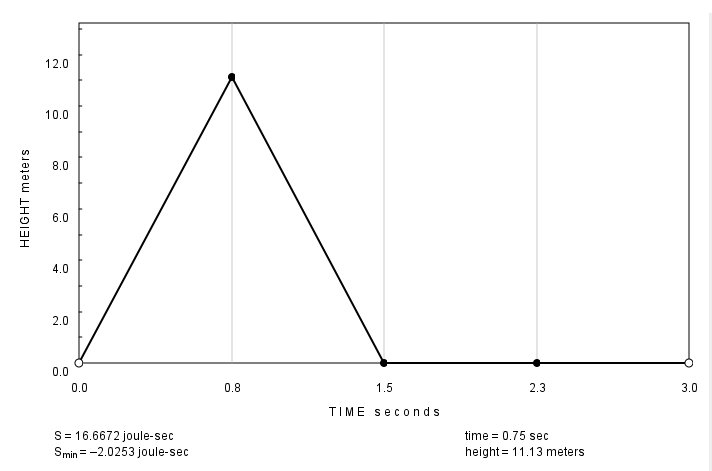
\includegraphics[scale=0.5]{apple1}
  \caption{Ejemplo de c\'alculo de la Acci\'on para una trayectoria arbitraria}
  \label{fig:apple1}
\end{figure}
Iterando el proceso se puede encontrar num\'ericamente (o a mano) la trayectoria que minimiza la acci\'on mostrada en la Fig.~\ref{fig:apple2}
\begin{figure}
  \centering
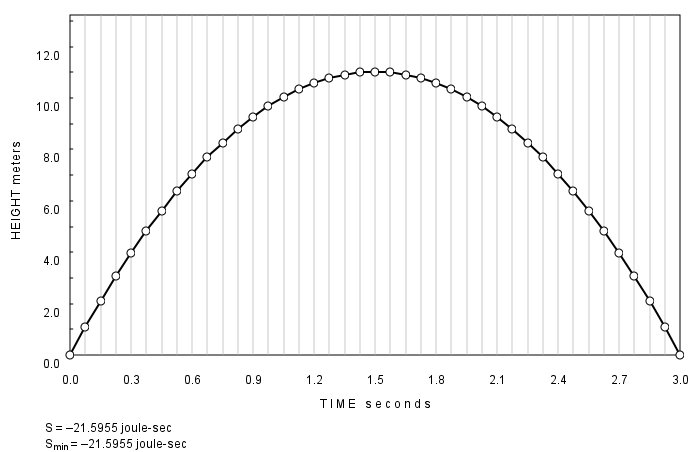
\includegraphics[scale=0.5]{apple2}
  \caption{Trayectoria que minimiza la Acci\'on}
\label{fig:apple2}
\end{figure}
Para una dimensi\'on podemos definir la densidad Lagrangiana como
\begin{equation}
  \mathcal{L}(q,\dot q,t)=\frac{\partial}{\partial q}L(q,\dot q,t)\qquad\text{or}\qquad L(q,\dot q,t)=\int\mathcal{L}(q,\dot q,t)dq.
\end{equation}
La ec.~\eqref{eq:la} puede escribirse entonces como
\begin{equation}
   S\left[q_i,\dot{q}_i\right] = \int \mathcal{L}(q_i(t), \dot{q}_i(t),t)\, dq\,dt.
\end{equation}
Para sistemas continuos es conveniente usar la densidad Lagrangiana. Abordaremos a continuaci\'on el sistema continuo correspondiente a la cuerda cl\'asica unidimensional para construir la densidad Lagrangiana correspondiente. A partir de ella demostraremos las ecuaciones de Euler Lagrange para dicho sistema.

%\left(\right)

\section{La cuerda cl\'asica unidimensional}
\label{sec:la-cuerda-clasica}

\begin{frame}[fragile,allowframebreaks]
Considere una cuerda de longitud $L$ formando un c\'\i rculo de radio $R$.
Es conveniente considerar un conjunto de $N$ part\'\i culas de masa $m$ a
lo largo de la circunferencia, unidas por resortes de longitud $l$ y
constante el\'astica $k$. Los modos vibracionales de la cuerda a lo
largo de la circunferencia se obtienen en l\'\i mite de $N\to\infty$ y $l\to0$ 
%noinstiki

\begin{figure} %noinstiki
  \centering %noinstiki
  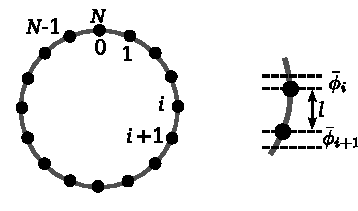
\includegraphics{cuerda} %noinstiki
  \caption{Modelo Cuerda} %noinstiki
  \label{fig:1string} %noinstiki
\end{figure} %noinstiki<div id="fig:1string">Figura cuerda: Modelo cuerda</div>
%noinstiki![cuerda](http://gfif.udea.edu.co/figfs/cuerda.png)
%noinstiki
De acuerdo a la figura 
\ref{fig:1string}, %noinstiki([cuerda](#fig:1string)),
si $\bar{\phi_i}=\bar{\phi}(z_i,t)$ es el
desplazamiento de la $i$--esima masa desde su posici\'on de equilibrio,
entonces el Lagrangiano del sistema de $N$ particulas y resortes es:
\begin{align}
  \label{eq:1strLsum} %noinstiki
  L&=\frac{1}{2}m\sum_{i=0}^{N-1}
  \left(
\frac{\partial\bar\phi_i}{\partial t}
  \right)^2-\frac{1}{2}k\sum_{i=0}^{N-1}
  \left(
\bar\phi_{i+1}-\bar\phi_{i}
  \right)^2,\\
  \label{eq:1strLsumdot} 
&=\frac{1}{2}m\sum_{i=0}^{N-1}
  \left(
    \dot{\bar{\phi_i}}
  \right)^2-\frac{1}{2}k\sum_{i=0}^{N-1}
  \left(
\bar\phi_{i+1}-\bar\phi_{i}
  \right)^2.
\end{align}
Si $\mu$ es la densidad de la cuerda, $T$ la tensi\'on y $v$ la velocidad, entonces
\begin{align}
  \label{eq:micromacro}
  \mu&=\frac{m}{l}\nonumber\\
  T&=kl\\
  v^2&=\frac{T}{\mu}.\nonumber
\end{align}
(\ref{eq:micromacro})
En el l\'\i mite $l\to0$ y $N\to\infty$, tenemos
\begin{equation}
  \label{eq:barf}
  \bar\phi_i=\bar\phi(z_i,t)\to\bar\phi(z,t),
\end{equation}
que representa la funci\'on de campo del desplazamiento de una masa
infinitesimal de su posici\'on de equilibrio. Entonces
\begin{align}
L&=\frac{1}{2}\sum_{i=0}^{N-1}\frac{m}{l}l
  \left(
    \dot{\bar{\phi_i}}
  \right)^2-\frac{1}{2}\sum_{i=0}^{N-1}(k l) l
  \left(
\frac{\bar\phi_{i+1}-\bar\phi_{i}}{l}
  \right)^2.\nonumber\\
&=\frac{1}{2}\sum_{i=0}^{N-1}\mu
  \left(
    \dot{\bar{\phi_i}}
  \right)^2l-\frac{1}{2}\sum_{i=0}^{N-1}T
  \left(
\frac{\bar\phi_{i+1}-\bar\phi_{i}}{l}
  \right)^2l.
\label{eq:1strLsumm}
\end{align}
En el l\'\i mite continuo $\sum(\cdots)\,l\to\int(\cdots)\,dz$, entonces 
\begin{equation}
\label{eq:238}
  L=\int_0^L\frac{1}{2}
\left[
  \mu\left(\frac{\partial\bar\phi}{\partial t}\right)^2- T\left(\frac{\partial\bar\phi}{\partial z}\right)^2
\right]dz=\int_0^L\mathcal{L}dz,
\end{equation}
con
\begin{equation}
  \label{eq:call1}
  \mathcal{L}=\frac{1}{2}
\left[
  \mu\left(\frac{\partial\bar\phi}{\partial t}\right)^2- T\left(\frac{\partial\bar\phi}{\partial z}\right)^2
\right],
\end{equation}
y
\begin{equation}
  \label{eq:Scall}
  S=\int\mathcal{L}\,dtdz.
\end{equation}
Definiendo
\begin{equation}
  \label{eq:barff}
  \phi=\sqrt{T}\bar\phi,
\end{equation}
tenemos
\begin{align}
  \label{eq:call2}
  \mathcal{L}(\partial\phi/\partial t,\partial\phi/\partial z)=&
\frac{1}{2}
\left[
  \frac{\mu}{T}\left(\frac{\partial\phi}{\partial t}\right)^2- \frac{T}{T}\left(\frac{\partial\phi}{\partial z}\right)^2
\right]\nonumber\\
=&\frac{1}{2}
\left[
  \frac{1}{v^2}\left(\frac{\partial\phi}{\partial t}\right)^2-\left(\frac{\partial\phi}{\partial z}\right)^2
\right],
\end{align}
\end{frame}
Note que:
\begin{align}
  \label{eq:dcalt}
  \frac{\partial}{\partial t}
  \left[
    \frac{\partial\mathcal{L}}{\partial
      (\partial\phi/\partial t)}
  \right]&=    \frac{1}{v^2}\frac{\partial^2\phi}{\partial t^2}\\
  \label{eq:dcalz} %noinstiki
  \frac{\partial}{\partial z}
  \left[
    \frac{\partial\mathcal{L}}{\partial
      (\partial\phi/\partial z)}
  \right]&= -\frac{\partial^2\phi}{\partial z^2}
\end{align}


Si en la ec.~\eqref{eq:1strLsumdot}, tomamos como coordenadas
generalizadas las $N$ $\dot{\bar{\phi_i}}$ y $\bar\phi_i$, entonces, podemos
obtener las ecuaciones de movimiento a partir de las ecuaciones de
Euler-Lagrange \eqref{eq:eel}:
\begin{equation}
  \label{eq:eelfi}
   \frac{d}{dt} \left ( \frac{\partial L}{\partial\dot{\bar{\phi_i}}} \right ) -
   \frac{\partial L}{\partial \bar\phi_i} = 0,
\qquad \text{$i=0$ hasta $N-1$}.
\end{equation}
En el l\'\i mite $l\to0$ y $N\to\infty$, y usando las ecs.~\eqref{eq:dcalt} 
y \eqref{eq:dcalz}, %noinstiki
\begin{align}
  \label{eq:emov1}
  \frac{d}{dt} \left( \frac{\partial L}{\partial\dot{\bar{\phi_i}}} \right)
  &=\frac{d}{dt} \left( m\dot{\bar{\phi_i}} \right)
= m\frac{\partial^2\bar{\phi_i}}{\partial t^2} \nonumber\\
&= T l\left(\frac{\mu}{T}\frac{\partial^2\bar{\phi_i}}{\partial t^2} \right)\nonumber\\
  &\to
  l\sqrt{T}
  \left(
    \frac{1}{v^2}\frac{\partial^2\phi}{\partial t^2}
  \right)\\
  \label{eq:eecalt} %noinstiki
  &=l\sqrt{T}\frac{\partial}{\partial t}
  \left[
    \frac{\partial\mathcal{L}}{\partial
      (\partial\phi/\partial t)}
  \right].
\end{align}
Para el segundo t\'ermino de la ec.~(\ref{eq:eelfi}) n\'otese que
\begin{align}
- \sum_{i=0}^{N-1}\left(\bar\phi_{i+1}-\bar\phi_{i}\right)^2= 
 &-\left(\bar\phi_{1}-\bar\phi_{0}\right)^2-\left(\bar\phi_{2}-\bar\phi_{1}\right)^2-\cdots
-\left(\bar\phi_{(i-1)+1}-\bar\phi_{i-1}\right)^2-\left(\bar\phi_{i+1}-\bar\phi_{i}\right)^2-\cdots\nonumber\\
 =&-\left(\bar\phi_{1}-\bar\phi_{0}\right)^2-\left(\bar\phi_{2}-\bar\phi_{1}\right)^2-\cdots
 -\left(\bar\phi_{i}-\bar\phi_{i-1}\right)^2-\left(\bar\phi_{i+1}-\bar\phi_{i}\right)^2-\cdots\nonumber\\
\end{align}
Entonces
\begin{align}
-\frac{\partial}{\partial\bar\phi_i}  \sum_{i=0}^{N-1}\left(\bar\phi_{i+1}-\bar\phi_{i}\right)^2
=&-2\left(\bar\phi_{i}-\bar\phi_{i-1}\right)-2\left(\bar\phi_{i+1}-\bar\phi_{i}\right)\times(-1)\nonumber\\
=&2l\left[\frac{\bar\phi_{i+1}-\bar\phi_{i}}{l}-\frac{\bar\phi_{i}-\bar\phi_{i-1}}{l}\right].\nonumber
\end{align}
Si $\bar{z}_i$ es el punto medio del intervalo entre $z_{i-1}$ y $z_i$, entonces en el l\'\i mite de $l\to0$,
\begin{align}
  -\frac{\partial}{\partial\bar\phi_i}  \sum_{i=0}^{N-1}\left(\bar\phi_{i+1}-\bar\phi_{i}\right)^2
  =&2l^2\left\{\frac{[\bar\phi(z_{i+1},t)-\bar\phi(z_{i},t)]/l}{l}-\frac{[\bar\phi(z_{i},t)-\bar\phi(z_{i-1},t)]/l}{l}\right\}\nonumber\\
&2l^2\left[\frac{\partial\bar\phi(\bar z_{i+1},t)/\partial z}{l}-\frac{\partial\bar\phi(\bar z_{i},t)/\partial z}{l}\right]\nonumber\\
  =&2l^2\frac{\partial^2\bar\phi}{\partial z^2}\nonumber\\
  \label{eq:129}
  \to&\frac{2l^2}{\sqrt{T}}\frac{\partial^2\phi}{\partial z^2}.
\end{align}
Usando las ecs.~(\ref{eq:129}) (\ref{eq:micromacro}), tenemos

\begin{align}
  \label{eq:emov2}
  \frac{\partial L}{\partial\bar{\phi_i}}
&=\frac{1}{2}k
\left[-\frac{\partial}{\partial\bar{\phi_i}}\sum_{i=0}^{N-1}\left(\bar\phi_{i+1}-\bar\phi_{i}\right)^2\right]
\nonumber\\
&\to\frac{1}{2}k\left(\frac{2l^2}{\sqrt{T}}\right)\frac{\partial^2\phi}{\partial z^2}
\nonumber\\
&\to  l\sqrt{T}
      \frac{\partial^2\phi}{\partial z^2}\\
  \label{eq:eecalz}
  &=-l\sqrt{T}\frac{\partial}{\partial z}
  \left[
    \frac{\partial\mathcal{L}}{\partial
      (\partial\phi/\partial z)}
  \right].
\end{align}
De las ecuaciones \eqref{eq:emov1} y \eqref{eq:emov2}, obtenemos la
ecuaci\'on de movimiento para el campo $\phi(z,t)$:
\begin{equation}
  \label{eq:econda1}
    \frac{1}{v^2}\frac{\partial^2\phi}{\partial t^2}-\frac{\partial^2\phi}{\partial z^2}=0,
\end{equation}
que corresponde a la ecuaci\'on de onda en una dimensi\'on. En tres
dimensiones obtendr\'\i amos:
\begin{equation}
  \label{eq:econda3}
    \frac{1}{v^2}\frac{\partial^2\phi}{\partial t^2}-\nabla^2\phi=0.
\end{equation}
De otro lado, de las ecuaciones 
\eqref{eq:eecalt} %noinstiki\eqref{eq:emov1}
y \eqref{eq:eecalz}, %noinstiki\eqref{eq:emov2},
obtenemos las ecuaciones de Euler-Lagrange para la densidad Lagrangiana
\begin{equation}
  \label{eq:eelcalls1}
\frac{\partial}{\partial t}
  \left[
    \frac{\partial\mathcal{L}}{\partial
      (\partial\phi/\partial t)}
  \right]+  \frac{\partial}{\partial z}
  \left[
    \frac{\partial\mathcal{L}}{\partial
      (\partial\phi/\partial z)}
  \right]=0.
\end{equation}
En tres dimensiones:
\begin{equation}
  \label{eq:eelcalls1m}
\frac{\partial}{\partial t}
  \left[
    \frac{\partial\mathcal{L}}{\partial
      (\partial\phi/\partial t)}
  \right]+\frac{\partial}{\partial x}
  \left[
    \frac{\partial\mathcal{L}}{\partial
      (\partial\phi/\partial x)}
  \right]+\frac{\partial}{\partial y}
  \left[
    \frac{\partial\mathcal{L}}{\partial
      (\partial\phi/\partial y)}
  \right]+\frac{\partial}{\partial z}
  \left[
    \frac{\partial\mathcal{L}}{\partial
      (\partial\phi/\partial z)}
  \right]=0.
\end{equation}
Definiendo
\begin{equation}
  \label{eq:xmu}
  x^\mu=(x^0,x^i)=(x^0,x^1,x^2,x^3)=(t,x,y,z) \qquad \mu=0,1,2,3,\quad i=1,2,3\,,
\end{equation}
en un sistema de unidades donde $x^0$ tenga las mismas unidades que
$x^i$, podemos expresar las ecuaciones de Euler-Lagrange que satisface
$\mathcal{L}(\partial\phi/\partial x^\mu)$, como
\begin{align*}
 \sum_\mu\frac{\partial}{\partial x^\mu}
  \left[
    \frac{\partial\mathcal{L}}{\partial
      (\partial\phi/\partial x^\mu)}
  \right]&=0\\
 \frac{\partial}{\partial x^\mu}
  \left[
    \frac{\partial\mathcal{L}}{\partial
      (\partial\phi/\partial x^\mu)}
  \right]&=0,
\end{align*}
donde, en la \'ultima ecuaci\'on se ha usado la convenci\'on de suma sobre
\'\i ndices repetidos. 

Si la densidad Lagrangiana depende tambi\'en directamente de $\phi$,
$\mathcal{L}(\partial\phi/\partial x^\mu,\phi)$, entonces la ecuaci\'on de Euler-Lagrange para
las coordenadas generalizadas  $\partial\phi/\partial x^\mu$ y $\phi$, es
\begin{equation}
\label{eq:eelcallf}
 \frac{\partial}{\partial x^\mu}
  \left[
    \frac{\partial\mathcal{L}}{\partial
      (\partial\phi/\partial x^\mu)}
  \right]-\frac{\partial\mathcal{L}}{\partial\phi}=0.
\end{equation}
\'Esta \'ultima ecuaci\'on se deducir\'a usando m\'etodos variacionales en la
secci\'on~\ref{sec:principio-de-minima-call}.

\begin{frame}[fragile,allowframebreaks]
La generalización de la densidad Lagrangiana a tres dimensiones esta dada por
\begin{align}
  \label{eq:dlc3d}
  \mathcal{L}(\partial\phi/\partial t,\partial\phi/\partial x,\partial\phi/\partial y,\partial\phi/\partial z)
=&\frac{1}{2}
\left[
  \frac{1}{v^2}\left(\frac{\partial\phi}{\partial t}\right)^2-\left(\frac{\partial\phi}{\partial x}\right)^2-\left(\frac{\partial\phi}{\partial y}\right)^2-\left(\frac{\partial\phi}{\partial z}\right)^2
\right],
\end{align}

\end{frame}

\section{Construción de Lagrangianos covariantes}

En está sección vamos a conectar la discusión sobre el Lagrangiano de las vibraciones de la cuerda con las tranformaciones de Lorentz de la relatividad especial. Dicho Lagrangiano tiene hasta ahora la siguiente dependencia funcional $\mathcal{L}(\partial_{\mu}\phi)$.

En la formulación de la teoría clásica de campos debemos asegurarnos de que todos los términos posibles perimtidos por la simetrías asociadas al campo estén presentes en la densidad Lagrangiana. De inmediato surge la pregunta: ¿Qué posibles términos de la forma $\partial_{\mu}\phi$ podrían estar presentes en Lagrangiano?. Antes de responder está pregunta, abordemos el problema algo más general donde la densidad Lagrangiana también depende del campo como mismo
\begin{align*}
  \mathcal{L}(\phi,\partial_\mu \phi)\,.
\end{align*}
En la ecuación~\eqref{eq:dlc3d}, teníamos un Lagragiano en función de $\partial_{\mu}\phi$, y haciendo $v\to c=1$, tenemos
\begin{align}
\label{eq:Lpr}
  \mathcal{L}(\partial_{\mu}\phi)
    =&\frac{1}{2}\left[
      {\partial_0\phi}\,{\partial_0\phi}-\sum_i{\partial_i\phi}\,{\partial_i\phi}
   \right]\nonumber\\
    =&\frac{1}{2}\left[
      {\partial_0\phi}\,{\partial^0\phi}+{\partial_i\phi}\,{\partial^i\phi}
   \right]\nonumber\\
   =&\frac{1}{2}{\partial_\mu\phi}\,{\partial^\mu\phi}\,.
\end{align}
donde se ha usado la convención de suma para índices repetidos. Note que para que la velocidad de propagación sea independiente del sistema de coordenadas se requiere su identificación con la velocidad de la luz. De modo que la queremos interpretar los términos de la densidad Lagrangiana como objetos invariantes, necesariamente se tiene que hacer en el contexto de la relatividad especial.




\section{Transformación de Lorentz para campos escalares}

El campo escalar esta definido por sus propiedades bajo transformaciones de Lorentz. Vamos a estudiar el comportamiento de un campo escalar bajo una transformación general de Lorentz:
\begin{align}
\label{eq:179qft}
  x^\mu\to {x'}^\mu={\Lambda^\mu}_\nu x^\nu\,,
\end{align}
Por definición, el campo escalar no cambia bajo la transformación de Lorentz, es decir, su forma funcional queda inalterada. Por consiguiente el campo escalar debe satisfacer que
\begin{align}
 \phi(x)\to  \phi'(x')=\phi(x)\,,
\end{align}
como se ilustra en la Fig.~\ref{fig:trasla}. La prima en $\phi$ representa el cambio intrínseco en el campo $\phi$ como consecuencia de la transformación. Definimos el cambio correspondiente como
\begin{align}
  \delta \phi(x)=\phi'(x)-\phi(x)\,.
\end{align}




Una transformación de Lorentz infinitesimal,
puede parametrizarse sin perdida de generalidad como
\begin{align}
  x^\mu\to{x'}^\mu=&x^\mu+\delta x^{\mu}\nonumber\\
\end{align}

Para visualizar más fácilmente la situación para un campo escalar, supongamos de momento que $\delta x^{\mu}$ corresponde  traslaci\'on espacio--temporal.

Tenemos
\begin{align}
  \phi'(x')&=\phi'(x+\delta x)\\
  &\approx\phi'(x)+\frac{\partial\phi'(x)}{\partial x^\mu}\delta x^\mu\\
  &=[\phi(x)+\delta\phi(x)]+\frac{\partial}{\partial x^\mu}[\phi(x)+\delta\phi(x)]\delta x^\mu\\
  &\approx\phi(x)+\delta\phi(x)+\frac{\partial\phi(x)}{\partial x^\mu}\delta x^\mu,
\end{align}
donde, por simplicidad, $\phi$ es un campo real. Entonces,
\begin{equation}
  \label{eq:Deltaf}
  \Delta\phi(x)\equiv\phi'(x')-\phi(x)=\delta\phi(x)+\frac{\partial\phi(x)}{\partial x^\mu}\delta x^\mu.
\end{equation}
Para una traslaci\'on, $\Delta\phi(x)=0$, ver figura 
\ref{fig:trasla}. %noinstiki([trasla](#fig:trasla)).
De modo que
\begin{equation}
  \label{eq:dmuxmu}
  \delta\phi=-(\partial_\mu\phi)\delta x^\mu,
\end{equation}
y la transformaci\'on del campo $\phi$ como consecuencia de la traslaci\'on es
\begin{align}
  \phi(x)\to\phi'(x)=\phi(x)-\delta\phi(x)=\phi(x)+(\partial_\mu\phi(x))\delta x^\mu\,.
\end{align}
%noinstiki

\begin{figure} %noinstiki
  \centering %noinstiki
  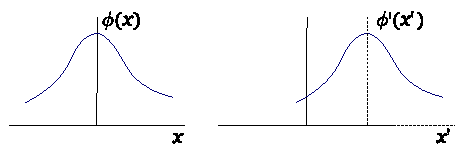
\includegraphics{trasla} %noinstiki
  \caption{Traslaci\'on de funci\'on y coordenadas en una dimensi\'on: $\phi(x)=\phi'(x')$ } %noinstiki
  \label{fig:trasla} %noinstiki
\end{figure} %noinstiki<div id="fig:trasla">Figura trasla:Traslaci\'on de funci\'on y coordenadas $\phi(x)=\phi(x')$ </div>
%noinstiki![trasla](http://gfif.udea.edu.co/figfs/trasla.png)
%noinstiki




Usando la ec.~\eqref{eq:179qft}, tenemos que
\begin{align}
    \phi'(x')=\phi(\Lambda^{-1}x')\,.
\end{align}
Esto es, el campo transformado, evaluado en el punto transformado, da el mismo valor que el campo evaluado en el punto antes de la transformación. 

\begin{frame}[fragile,allowframebreaks]

%Therefore, for an arbitrary space-time point we have that the scalar field transforms under a Lorentz transformation as
Por consiguiente, para un punto del espacio tiempo arbitrario tenemos
que el campo escalar transforma bajo una transformación de Lorentz como
\begin{align}
  \label{eq:scalarlorentz}
 \phi(x)\to  \phi'(x)=\phi(\Lambda^{-1}x)\,.
\end{align}
\end{frame}

Para comprobar la invarianza de Lorentz de la Acción para el campo escalar, necesitamos las propiedades de transformación para $\partial_\mu$. En conveniente invertir la ec.~\eqref{eq:179qft}
\begin{align}
  {\left(\Lambda^{-1}\right)^\mu}_\alpha{x'}^\alpha=&{\left(\Lambda^{-1}\right)^\mu}_\alpha{\Lambda^\alpha}_\nu x^\nu\nonumber\\
=&\delta^\mu_\nu x^\nu\nonumber\\
=&x^\mu\,,
\end{align}
\begin{align}
  \frac{1}{{x'}^\nu}= {\left(\Lambda^{-1}\right)^\mu}_\nu\frac{1}{x^\mu}\,,
\end{align}
o
\begin{align}
  \label{eq:183qft}
    \frac{1}{{x'}^\mu}= {\left(\Lambda^{-1}\right)^\nu}_\mu\frac{1}{x^\nu}\,,
\end{align}
de modo que la transformación de Lorentz para $\partial_\mu=\partial/\partial x^\mu$, es
\begin{align}
  \label{dmulrtran}
   \frac{\partial}{{\partial x'}^\mu}=& {\left(\Lambda^{-1}\right)^\nu}_\mu\frac{\partial}{\partial x^\nu}\nonumber\\
   {\partial\,}'_\mu=& {\left(\Lambda^{-1}\right)^\nu}_\mu\partial_\nu\,,
\end{align}
Podemos ahora demostrar que la Acción obtenida del Lagrangiano en la ec.\eqref{eq:Lpr} es invariante bajo transformaciones de Lorentz haciendo uso de la ec.~(\ref{eq:Lambdacontra}). Para hacer la demostración más general, podemos agregar una función general que solo dependa del campo $\phi$ pero no de sus derivadas, $V(\phi)$
\begin{align}
  \mathcal{L}(\phi(x),\partial_{\mu}\phi(x))\to  \mathcal{L}'=& \frac{1}{2}\partial'_\mu\phi'(x)\partial^{'\mu}\phi'(x)-V(\phi'), \nonumber\\
  =&{\left(\Lambda^{-1}\right)^\nu}_\mu g^{\mu \rho}{\left(\Lambda^{-1}\right)^\sigma}_\rho \partial_\nu\phi(\Lambda^{-1}x) \partial_\sigma \phi(\Lambda^{-1}x) -V(\phi')\nonumber\\
  =& g^{\nu \sigma}\partial_\nu\phi(\Lambda^{-1}x) \partial_\sigma \phi(\Lambda^{-1}x) -V(\phi(\Lambda^{-1}x))\nonumber\\
  =& \partial_\nu\phi(\Lambda^{-1}x) \partial^{\nu} \phi(\Lambda^{-1}x) -V(\phi(\Lambda^{-1}x)) \nonumber\\
  =&\mathcal{L}(\phi(\Lambda^{-1}x),\partial_{\mu}\phi(\Lambda^{-1}x))\,.
\end{align}
Ya que la Acción involucra la integración sobre todos los puntos, esta es invariante bajo transformaciones de Lorentz. Explícitamente
\begin{align}
  S\to S'=\int d^4x\, \mathcal{L}
\end{align}

Note que en unidades naturales
\begin{align}
  [S]=[\hbar]=1,
\end{align}
y ya que $[d^4x]=E^{-4}$, entonces
\begin{align}
  [\mathcal{L}]=E^{4}\,.
\end{align}
Como $[\partial_{\mu}]=E$, entonces
\begin{align}
  [\phi]=E\,.
\end{align}

\section{Principio de mínima acción para campos}
Hemos visto que la acción para una oscilación mecánica en tres dimensiones se puede escribir en una notación similar a la del producto escalar de un cuadrivector de Lorentz $\partial_\mu\phi$. Cuando dicho campo se interpreta como un campo fundamental, es decir, que su velocidad de propagación es independiente de los sistemas de referencia inerciales, entonces la Acción queda invariante bajo dicho producto escalar. También hemos visto que adicionar una función del campo $V(\phi)$, la invarianza de la acción se mantiene.

Establecemos el \emph{principio de mínima acción para campos} de la siguiente manera: La acción más general posible para un conjunto de campos contiene todos los posibles productos escalares entres los campos y sus derivadas, con las siguientes restricciones
\begin{enumerate}
\item La dimensión de los campos y derivadas en cada término de la correspondiente densidad lagrangiana debe ser menor o igual a cuatro.
\item La densisdad Lagrangiana no debe contener derivadas altas (máximo dos derivadas)
\item Los campos fundamentales se deben anular a espacio infinito.
\end{enumerate}
Con estas restricciones es suficiente mantener los primeros cuatro términos de la expansión de Taylor de $V(\phi)$ (el término constante se puede remover redefiniendo el estado de mínima energía)
\begin{align}
  V(\phi)=a \phi + b\phi^2+c\phi^4+d\phi^4\,,
\end{align}

La última condición excluye términos del tipo
\begin{align}
  \partial_\mu \partial^\mu phi\,,   \phi\partial_\mu \partial^\mu phi\,.
\end{align}
De modo que la densidad Lagrangiana más general posible para un campo escalar real es
\begin{align}
  \frac{1}{2}{\partial_\mu\phi}\,{\partial^\mu\phi}+a \phi + b\phi^2+c\phi^4+d\phi^4\,.
\end{align}

Realizaciones propuestas para este campo escalar incluye el de un campo de materia oscura con un potencial tipo oscilador armónico.
% figura
Pero una realización ya encontrada en la naturaleza corresponde al campo de Higgs con un potencial tipo ruptura expontánea de vacio

Una realización física para la acción del campo escalar real con un potencia escalar tipo ``slow-roll''  corresponde al campo del inflatón en cosmología.

\section{Campo escalar complejo}


Para un campo complejo con invarianza de fase, el potencial $V(\phi,\phi^{*})$ es único:
\begin{align}
\label{eq:cef}
  \mathcal{L}=\partial_{\mu}\phi^{*} \partial^{\mu}\phi-m^2\phi^{*}\phi+\lambda \left(\phi^{*}\phi \right)^2\,.
\end{align}
En efecto, la densidad Lagrangiana y por consiguiente la Acción, son invariante bajo la transformación
\begin{align}
  \phi\to \phi'=\operatorname{e}^{i\theta}\phi\,,\qquad \text{$\theta$ constante}\,.
\end{align}
Para $\theta$ infinitesimal
\begin{align}
\label{eq:deltaphi}
  \delta\phi=\phi'-\phi=i\theta\phi
\end{align}



Por lo tanto
\begin{align}
  \left[ m \right]=&E& \left[ \lambda \right]=&1\,.
\end{align}


Más adelente justificaremos por qué no hay potencias con dimensiones mayor a $E^{4}$ del campo $\phi$ en la ec.~\eqref{eq:cef}. No se consideran términos con derivadas superiores porque al igual que en mecánica clásica pueden generar inestabilidades. Por lo tanto, los únicos términos con derivadas que dejen invariante la acción bajo transformaciones de Lorentz son (el primero sólo es posible para un campo real):
\begin{align}
  \partial_{\mu}\partial^{\mu}\phi,\qquad \phi^{*}\partial_{\mu}\partial^{\mu}\phi\,.
\end{align}
Una densidad Lagrangiana incluyendo estos términos se puede reescribir en términos de la densidad Lagranginan en la ec.~\eqref{eq:cef}, hasta una deriva total. Por ejemplo
\begin{align}
  \mathcal{L}_{\text{new}}=&-\phi^{*}\partial_{\mu}\partial^{\mu}\phi-m^2\phi^{*}\phi+\lambda \left(\phi^{*}\phi \right)^2\,\nonumber\\
=&\partial_{\mu}\phi^{*}\partial^{\mu}\phi\,-\partial_{\mu}\left(\phi^{*}\partial^{\mu}\phi\right)-m^2\phi^{*}\phi+\lambda \left(\phi^{*}\phi \right)^2\,\nonumber\\
=&\mathcal{L}-\partial_{\mu}\left(\phi^{*}\partial^{\mu}\phi\right)\,.
\end{align}
En general, si comparamos dos acciones que difieran en la derivada total de algún $X^{\mu}$ (en el caso anterior $X^{\mu}=-\phi^{*}\partial^{\mu}\phi$)
\begin{align}
  S_{\text{new}}=S+\int \partial_{\mu}\left(\phi^{*}\partial^{\mu}\phi\right)d^4x\,.
\end{align}
Veremos más adelante que la integral de una derivada total, con las condiciones de frontera adecuadas, no contribuye a la Acción.





\section{Problema variacional de Noether}

\section{Tipos de conservación }
Un sistema binario de estrellas conserva la energía globalmente, pero un sistema binario de estrellas de neutrones donde los efectos relativistas sean importante violan la energía globalmente, es decir, el sistema se vuelve inestable. ¿Qué pasa con la conservación de la energía en ese último caso?

\section{Teoremas}



Seguiremos la discusión basada en \cite{Brading:2000hc,Brading:2003nv,Sundermeyer:2014kha}.

Un campo escalar complejo es equivalente a dos campos escalares independientes de la misma masa asociados a un parámetro de transformación $\theta$. Para $N$ campos asociados a un parámetro de transformación $\theta$ , la dependencia explicita e implicita de la densidad Lagrangiana da lugar al funcional de Acción
\begin{equation}
  S[\phi_i,\partial_\mu\phi_i;x]=\int_{R}d^4x\,\mathcal{L}(\phi_i,\partial_\mu\phi_i;x)
\end{equation}
El problema variacional de Noether, que es diferente al principio de Hamilton, puede ser establecido en los siguientes términos

¿Cuales son las condiciones generales que se deben satisfacer para que una dada variación en la variables explícitas e implicitas dejen a la Acción invariante, y de aquí $\delta S=0$, donde $\delta S$ puede o no contener un término de frontera?

Definiendo el cambio interno en el campo como en \eqref{eq:deltaphi}
\begin{align}
  \delta\phi_i(x)=\phi'(x)-\phi(x)\,,
\end{align}
y el cambio en $x$ bajo una transformación de Lorentz infinitesimal como
\begin{align}
\label{eq:deltax}
  x\to x'=x+\delta x
\end{align}
tenemos que la variación en las variables dependientes e independientes de la Acción son
\begin{align}
   \delta S=&\int_{R}d^4x'\,\mathcal{L} \left( \phi_{i}',\partial_{\mu}\phi'_i;x' \right)- \int_{R}d^4x\,\mathcal{L} \left( \phi_{i}(x),\partial_{\mu}\phi_i(x);x \right) \nonumber\\
     =&\int_{R}\frac{\partial x'}{\partial x}d^4x\,\mathcal{L} \left( \phi_{i}+\delta\phi_i,\partial_{\mu}(\phi_i+\delta\phi_i);x+\delta x \right)- \int_{R}d^4x\,\mathcal{L} \left( \phi_{i},\partial_{\mu}\phi_i;x \right)\,
\end{align}
Derivando \eqref{eq:deltax},
\begin{align}
     \delta S =&\int_{R} \left[ 1+\partial_{\mu} \left( \delta x^{\mu}  \right)\right]  d^4x\,\left\{ \mathcal{L}(\phi_i,\partial_{\mu}\phi_i;x)+\sum_i \left[ \frac{\partial\mathcal{L}}{\partial\phi_i}\delta\phi_{i} +\frac{\partial\mathcal{L}}{\partial(\partial_{\mu}\phi_i)}\partial_{\mu}(\delta\phi_{i}) \right]+\left( \partial_{\mu}\mathcal{L} \right)\delta x^{\mu} \right\}\nonumber\\
      &- \int_{R}d^4x\,\mathcal{L} \left( \phi_{i},\partial_{\mu}\phi_i;x \right) \nonumber\\
     =&\int_{R} d^4x\,\left[ \partial_{\mu} \left( \delta x^{\mu}  \right)\right] \mathcal{L} + \int_{R}d^4x\,\left\{\sum_i \left[ \frac{\partial\mathcal{L}}{\partial\phi_i}\delta\phi_{i} +\frac{\partial\mathcal{L}}{\partial(\partial_{\mu}\phi_i)}\partial_{\mu}(\delta\phi_{i}) \right]+\left( \partial_{\mu}\mathcal{L} \right)\delta x^{\mu} \right\}\nonumber\\
     =&\int_{R} d^4x\,\partial_{\mu} \left(\mathcal{L} \delta x^{\mu}  \right)  + \int_{R}d^4x\,\sum_i \left\{ \frac{\partial\mathcal{L}}{\partial\phi_i}\delta\phi_{i} +\partial_{\mu} \left[ \frac{\partial\mathcal{L}}{\partial(\partial_{\mu}\phi_i)}\delta\phi_{i} \right]-\partial_{\mu} \left[ \frac{\partial\mathcal{L}}{\partial(\partial_{\mu}\phi_i)}\right]\delta\phi_{i}  \right\}\nonumber\\
\end{align}
La condición $\delta S=0$ implica que
\begin{align}
\label{eq:masterint}
\int \operatorname{d}^4x  \sum_i \mathcal{E}_i \delta\phi_i =\int \operatorname{d}^4x \sum_i \partial_{\mu} B^{\mu}_{i}\,,
\end{align}
o

\begin{align}
  \sum_i \mathcal{E}_i \delta\phi_i = \sum_i \partial_{\mu} B^{\mu}_{i}\,,
\end{align}
donde
\begin{align}
\label{eq:master2}
  \mathcal{E}_i=&\partial_{\mu} \left[ \frac{\partial\mathcal{L}}{\partial(\partial_{\mu}\phi_i)}\right]-\frac{\partial\mathcal{L}}{\partial\phi_i} & B^{\mu}_i=\mathcal{L} \delta x^{\mu} + \frac{\partial\mathcal{L}}{\partial(\partial_{\mu}\phi_i)}\delta\phi_{i} 
\end{align}


\section{Ecuaciones de Euler-Lagrange}
%%TODO: Mejorar
El teorema de Gauss establece que
\begin{equation}
\int_V\boldsymbol{\nabla}\cdot\mathbf{A}\,d^3x=
 \int_S\mathbf{A}\cdot d\mathbf{S}\,.
\end{equation}
Generalizado a cuatro dimensiones, tenemos
\begin{align}
\int_{\mathcal{V}} \operatorname{d}^4x\,\partial_{\mu} \eta^{\mu}=
\int_{\sigma} \operatorname{d}\sigma_{\mu} \eta^{\mu}\,,   
\end{align}
donde $\mathcal{V}$ es el volumen en cuatro dimensiones (4D) y $\sigma$ la correspondiente hipersuperficie en tres dimensiones.

Aplicando las condiciones de Frontera usando  el teorema de Gauss en 4D en el lado derecho de \eqref{eq:masterint},
%detalles
es claro que la integral de frontera se anula si imponemos que la variación tanto de la coordenadas, $\delta x^{\mu}$, como de los campos, $\delta \phi_{i}$ , en la frontera se hagan cero. Esto es equivalente a la anulación de las trayectorias en los extremos para la Acción en mecánica clásica, 

Obtenemos entonces las ecuaciones de Euler-Lagrange para cada campo $\phi_i$
\begin{align}
\label{eq:eelcallfmu}
  \partial_{\mu} \left[ \frac{\partial\mathcal{L}}{\partial(\partial_{\mu}\phi_i)}\right]-\frac{\partial\mathcal{L}}{\partial\phi_i}=0
\end{align}

La misma condición de nulidad de los campos en la frontera permite establecer que una densidad Lagrangiana modificada con una deriva total
\begin{align}
  \mathcal{L}'=\mathcal{L}+\partial_\mu(\eta^{\mu}(x))
\end{align}
donde $\eta^{\mu}(x)$ es cualquier función de los campos de la densidad Lagrangiana original que también sea cero sobre la frontera, da lugar a la Acci\'on
\begin{align}
  S'=\int_{R}d^4x\,\mathcal{L}'=&\int_{R}d^4x\,\mathcal{L}+\int_R d^4x\,\partial_\mu\eta^{\mu}\nonumber\\
  =&\int_{R}d^4x\,\mathcal{L}+\int_\sigma \eta^{\mu} d\sigma_{\mu}\nonumber\\
  =&S\,,
\end{align}
para una hipersuperficie suficientemente grande. De modo que dos densidades lagrangianas que difieran solo en derivadas totales dan lugar a la misma Acci\'on.

Usando el principio de m\'\i nima acci\'on en t\'erminos del campo $\phi$, tenemos que para la densidad Lagrangiana~\eqref{eq:call2}
\begin{align}
  \mathcal{L}=&\frac{1}{2}  \left[
  \frac{1}{v^2}\left(\frac{\partial\phi}{\partial t}\right)^2-\left(\frac{\partial\phi}{\partial z}\right)^2
\right],
\end{align}
las ecuaciones de Euler-Lagrange~\eqref{eq:eelcallfmu}
\begin{align}
  \partial_0\left[\frac{\partial\mathcal{L}}{\partial(\partial_0\phi)}\right]+
\partial_3\left[\frac{\partial\mathcal{L}}{\partial(\partial_3\phi)}\right]
-\frac{\partial\mathcal{L}}{\partial\phi}=&0\nonumber\\
  \frac{\partial}{\partial t}\left[\frac{\partial\mathcal{L}}{\partial(\partial\phi/\partial t)}\right]+
\frac{\partial}{\partial z}\left[\frac{\partial\mathcal{L}}{\partial(\partial\phi/\partial z)}\right]
=&0\nonumber\\
 \frac{1}{v^2}\frac{\partial}{\partial t}\left[\frac{\partial\phi}{\partial t}\right]
-\frac{\partial}{\partial z}\left[\frac{\partial\phi}{\partial z}\right]=&0\nonumber\\
 \frac{1}{v^2}\frac{\partial^2\phi}{\partial t^2}-\frac{\partial^2\phi}{\partial z^2}=&0\,,
\end{align}
que corresponde a la ec.~\eqref{eq:econda1}.

Generalizando a tres dimensiones vemos que la ecuaci\'on para una onda propagandose a una velocidad $v$, eq.~\eqref{eq:econda3},  
\begin{align}
     \partial_{\mu}\partial^{\mu}\phi=&0 \nonumber\\
     \frac{1}{v^2}\frac{\partial^2\phi}{\partial t^2}-\nabla^2\phi=&0\,,
\end{align}
proviene de la densidad Lagrangiana (hasta derivadas totales) dada por la ec.~\eqref{eq:Lpr}.

\section{Simetrías internas}
La virtud del trabajo de Noether~\cite{Noether} fue separar los resultados  en los casos de grupos de simetrías globales en los cuales el parámetro de transformación no depende del punto del espacio tiempo (como es el caso de las transformaciones a velocidad constante la relatividad especial: $v=\text{cte}$) del caso en que los grupos de simetría dependan del punto del espacio-tiempo (como los sistemas acelerados de la relatividad general donde la velocidad depende el punto del espacio-tiempo: $v(x)$).

En el caso de teorías de campos estamos más interesados en simetría de espacios internos como puede ser el cambio de fase de la función de onda en la ecuación de Schrödinger. Un cambio de fase, $\theta$, es un caso particular del parámetro de la transformación. En general el parámetro de una transformación interna puede ser constante, $\theta=\text{cte}$, que corresponde a una transformación de fase  \emph{global}, o depender del punto del espacio tiempo, $\theta(x)$, que corresponde  a una transformación  de fase \emph{local}. Las simetrías internas estan caracterizadas por la condición $\delta x^\mu=0$ 

Nos enfocaremos en esta sección en la formulación de los dos teoremas de Noether para el caso de simetrías internas globales y locales.   


Si la transformación depende de algún parámetro $\theta$ continuo, entonces podemos garantizar la existencia de un parámetro infinitesimal tal que
\begin{align}
\label{eq:infdt}
 \delta\phi_i= a_{i}\left( \phi_{i},\partial_{\mu}\phi_{i} \right) \theta(x)+b^{\nu}_i \left( \phi_{i},\partial_{\mu}\phi_{i} \right) \partial_{\nu}\theta(x)\,,
\end{align}

Para concretar, consideremos como transformación interna el cambio de fase de una función compleja
\begin{align}
  \phi\to \phi'=\operatorname{e}^{i\theta}\phi\,,  
\end{align}
Para un $\theta$ suficientemente pequeño
\begin{align}
  \phi'=&\operatorname{e}^{i\theta}\phi \nonumber\\
    \approx&(1+i \theta)\phi \nonumber\\
    \approx&\phi+i \theta\, \phi\,.
\end{align}
Definimos el cambio interno en la función como
\begin{align}
  \delta\phi\equiv \phi'-\phi\,,
\end{align}
y para el cambio infinitesimal del campo y su complejo conjugado, tenemos que haciendo $\phi_1=\phi$ y $\phi_2=\phi^{*}$
\begin{align}
  \delta\phi=&a_1 \theta\,, &  \delta\phi^{*}=&  a_2 \theta\,, 
\end{align}
donde
\begin{align}
  a_1=& i\phi \,, & a_2=&-i\phi^{*}\,.
\end{align}
Ademas, para este caso
\begin{align}
  b_1^\nu=b_2^\nu=0\,.
\end{align}



\section{Primer teorema de Noether}

Consideremos primero el caso en el que el parámetro de la transformación $\theta=\text{cte}$. Como $\partial_{\nu}\theta=0$ en ese caso
\begin{align}
\label{eq:infdt}
 \delta\phi_i= a_{i}\left( \phi_{i},\partial_{\mu}\phi_{i} \right) \theta(x)\,.
\end{align}



%Demostrar el primer teorema de Noether

Generalizando al caso de una transformación con varios parámetros, tendremos la formulación del primer teorema de Noether para simetrías internas:

\textbf{Teorema 1}: Si la acción $S$ es invariante bajo un grupo continuo de simetrías globales que dependen suavemente de $\rho$ parámetros independientes $\theta_{\alpha}=\text{cte}$ ($\alpha=1,2,\ldots, \rho$), tal que $\delta\phi_i=a_{\alpha i}\theta^{\alpha}$, entonces existen las $\rho$ relaciones
\begin{align}
\sum_{i}\mathcal{E}_i a_{\alpha i}\equiv \partial_{\mu} j^{\mu}_{\alpha}\,,  
\end{align}
donde
\begin{align}
j^{\mu}_{\alpha}\equiv \sum_{i}B^{\mu}_i=\sum_{i}  \frac{\partial\mathcal{L}}{\partial(\partial_{\mu}\phi_i)}a_{\alpha i}
\end{align}

\emph{Demostración}:  De la ec.~\eqref{eq:master2}
\begin{align}
\label{eq:varprin}
  \sum_i \mathcal{E}_i \delta\phi_i =&\sum_{i} \partial_{\mu} \left[\frac{\partial\mathcal{L}}{\partial(\partial_{\mu}\phi_i)}\delta\phi_{i}  \right] \nonumber\\
  \sum_i \mathcal{E}_i a_{\alpha i}\theta^{\alpha} =&\sum_{i} \partial_{\mu} \left[\frac{\partial\mathcal{L}}{\partial(\partial_{\mu}\phi_i)} a_{\alpha i}\theta^{\alpha}  \right] \nonumber\\
  \sum_i \mathcal{E}_i a_{\alpha i}\theta^{\alpha} =&\sum_{i} \partial_{\mu} \left[\frac{\partial\mathcal{L}}{\partial(\partial_{\mu}\phi_i)} a_{\alpha i}  \right]\theta^{\alpha}\,.
\end{align}
Igualando para cada $\theta^{\alpha}$
\begin{align}
    \sum_i \mathcal{E}_i a_{\alpha i} =&\sum_{i} \partial_{\mu} \left[\frac{\partial\mathcal{L}}{\partial(\partial_{\mu}\phi_i)} a_{\alpha i}  \right]
\end{align}

Si inponemos que las ecuaciones de Euler-Lagrange se satisfagan, es decir
\begin{align}
  \mathcal{E}_i=0\,,
\end{align}
obtenemos $\alpha$-\emph{ecuaciones de continuidad}
\begin{align}
  \partial_{\mu} j^{\mu}_{\alpha}=0\,.
\end{align}

Para entender el significado físico de la ecuación de continuidad consideremos la cuadri-corriente asociada a un único parámetro constante $\theta$, como en el caso de un campo escalar complejo y su correspondiente conjugado. Expandiendo la ecuación de continuidad en sus componentes espaciales y temporales tenemos que
\begin{align}
  \partial_0 j^0+ \partial_i j^i=&0\,,&\text{suma sobre $i$}\nonumber\\
  \frac{\partial j^0}{\partial t}+ \boldsymbol{\nabla}\cdot\boldsymbol{j}=&0\,.
\end{align}
Integrando sobre el volumen y aplicando el teorema de Gauss
\begin{align}
  \int_V \operatorname{d}^3x\,\frac{\partial j^0}{\partial t}
+\int_S \boldsymbol{j}\cdot \boldsymbol{S}=&0\,.
\end{align}
Si interpretamos $j^0$ como la densidad, $\rho$, de una cierta carga $Q$, tal que
\begin{align}
  Q=\int_{V} \operatorname{d}^3x\, j^0= \int_{V} \operatorname{d}^3x\, \rho\,,
\end{align}
entonces, si escogemos $S$ como una superficie suficientemente grande para contener toda la distribución de carga $Q$ en su interior, tendremos que la integral sobre la superficie se anula y por consiguiente
\begin{align}
  \int_V \operatorname{d}^3x\,\frac{\partial j^0}{\partial t}=&
\frac{\operatorname{d}}{\operatorname{d}t}\int_V \operatorname{d}^3x\,\rho \nonumber\\
=&\frac{\operatorname{d}Q}{\operatorname{d}t}\nonumber\\
  =&0\,.
\end{align}
Es decir, que la carga es independiente del tiempo, y por lo tanto se conserva.

Una consecuencia del primer teorema de Noether es que por cada simetría global de la Acción existe una carga conservada. 

Cuando la conservación de la carga requiera de que las ecuaciones de Euler-Lagrange se satisifagan, diremos que la conservación de la carga es \emph{propia}.

% \subsection{Teorema de Noether para simetr\'\i as externas}

% Si $a^\mu$ es constante (un an\'alisis m\'as general es hecho en \cite{r})
% \begin{equation}
%   d^4x'=d^4x
% \end{equation}
% En este caso, asumiendo que el campo satisface las ecuaciones de
% Euler-Lagrange y usando la ec.~\eqref{eq:dmuxmu} y (\ref{eq:eelcallfmu}) tenemos
% \begin{align}
%   \delta S&=\int_{R}d^4x\,\mathcal{L}(\phi',\partial_\mu\phi',x')-\int_{R}d^4x\,\mathcal{L}(\phi(x),\partial_\mu\phi(x),x)\nonumber\\
%   &=\int_{R}d^4x\,\mathcal{L}(\phi+\delta\phi,\partial_\mu\phi+\partial_\mu(\delta\phi),x+\delta a)-\int_{R}d^4x\,\mathcal{L}\nonumber\\
%   &\approx\int_{R}d^4x\,
%   \left[\mathcal{L}+
%     \frac{\partial\mathcal{L}}{\partial\phi}\delta\phi+\frac{\partial\mathcal{L}}{\partial(\partial_\mu\phi)}\partial_\mu(\delta\phi)+
%     (\partial_\mu\mathcal{L})\delta a^\mu\right]-\int_{R}d^4x\,\mathcal{L}\nonumber\\
%   &=\int_{R}d^4x\,
%   \left[
%     \frac{\partial\mathcal{L}}{\partial\phi}\delta\phi+\frac{\partial\mathcal{L}}{\partial(\partial_\mu\phi)}\partial_\mu(\delta\phi)+
%     (\partial_\mu\mathcal{L})\delta a^\mu\right]\nonumber\\
%   &=\int_{R}d^4x\,
%   \left\{ 
%     \left[\partial_\mu\left(\frac{\partial\mathcal{L}}{\partial(\partial_\mu\phi)}
%     \right)\right]\delta\phi+\frac{\partial\mathcal{L}}{\partial(\partial_\mu\phi)}\partial_\mu(\delta\phi)+
%     (\partial_\mu\mathcal{L})\delta a^\mu\right\}\nonumber\\
%   &=\int_{R}d^4x\left\{ 
%     \partial_\mu\left[\frac{\partial\mathcal{L}}{\partial(\partial_\mu\phi)}\delta\phi\right]
%   +(\partial_\mu\mathcal{L})\delta a^\mu\right\}\nonumber\\
%   &=\int_{R}d^4x\,
%     \partial_\mu\left[
%       -\frac{\partial\mathcal{L}}{\partial(\partial_\mu\phi)}(\partial_\nu\phi)
%       +\delta^\mu_\nu\mathcal{L}
%     \right]\delta a^\nu\nonumber\\
%     \label{eq:2}
%   &=\int_{R}d^4x\,
%   \left(
%     \partial_\mu T^\mu_\nu
%   \right)\delta a^\nu=0.
% \end{align}



% \subsection{Teorema de Noether para simetr\'\i as externas}
% \begin{frame}[fragile,allowframebreaks]
% Para el caso de una simetr\'\i a externas, por ejemplo la correspondiente a una traslaci\'on espacio--temporal
% \begin{align}
%   x^\mu\to{x'}^\mu=&x^\mu+\delta a^\mu\nonumber\\
%   \delta x^\mu=&\delta a^\mu
% \end{align}

% tenemos
% \begin{align}
%   \phi'(x')&=\phi'(x+\delta a)\\
%   &\approx\phi'(x)+\frac{\partial\phi'(x)}{\partial x^\mu}\delta a^\mu\\
%   &=[\phi(x)+\delta\phi(x)]+\frac{\partial}{\partial x^\mu}[\phi(x)+\delta\phi(x)]\delta a^\mu\\
%   &\approx\phi(x)+\delta\phi(x)+\frac{\partial\phi(x)}{\partial x^\mu}\delta a^\mu,
% \end{align}
% donde, por simplicidad, $\phi$ es de nuevo un campo real. Entonces,
% \begin{equation}
%   \label{eq:Deltaf}
%   \Delta\phi(x)\equiv\phi'(x')-\phi(x)=\delta\phi(x)+\frac{\partial\phi(x)}{\partial x^\mu}\delta a^\mu.
% \end{equation}
% Para una traslaci\'on, $\Delta\phi(x)=0$, ver figura 
% \ref{fig:trasla}. %noinstiki([trasla](#fig:trasla)).
% De modo que
% \begin{equation}
%   \label{eq:dmuxmu}
%   \delta\phi=-(\partial_\mu\phi)\delta a^\mu,
% \end{equation}
% y la transformaci\'on del campo $\phi$ como consecuencia de la traslaci\'on es
% \begin{align}
%   \phi(x)\to\phi'(x)=\phi(x)-\delta\phi(x)=\phi(x)+(\partial_\mu\phi(x))\delta a^\mu\,.
% \end{align}
% %noinstiki

% \begin{figure} %noinstiki
%   \centering %noinstiki
%   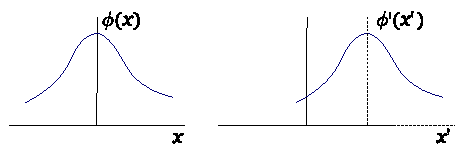
\includegraphics{trasla} %noinstiki
%   \caption{Traslaci\'on de funci\'on y coordenadas en una dimensi\'on: $\phi(x)=\phi'(x')$ } %noinstiki
%   \label{fig:trasla} %noinstiki
% \end{figure} %noinstiki<div id="fig:trasla">Figura trasla:Traslaci\'on de funci\'on y coordenadas $\phi(x)=\phi(x')$ </div>
% %noinstiki![trasla](http://gfif.udea.edu.co/figfs/trasla.png)
% %noinstiki
% Si $a^\mu$ es constante (un an\'alisis m\'as general es hecho en \cite{r})
% \begin{equation}
%   d^4x'=d^4x
% \end{equation}
% En este caso, asumiendo que el campo satisface las ecuaciones de
% Euler-Lagrange y usando la ec.~\eqref{eq:dmuxmu} y (\ref{eq:eelcallfmu}) tenemos
% \begin{align}
%   \delta S&=\int_{R}d^4x\,\mathcal{L}(\phi',\partial_\mu\phi',x')-\int_{R}d^4x\,\mathcal{L}(\phi(x),\partial_\mu\phi(x),x)\nonumber\\
%   &=\int_{R}d^4x\,\mathcal{L}(\phi+\delta\phi,\partial_\mu\phi+\partial_\mu(\delta\phi),x+\delta a)-\int_{R}d^4x\,\mathcal{L}\nonumber\\
%   &\approx\int_{R}d^4x\,
%   \left[\mathcal{L}+
%     \frac{\partial\mathcal{L}}{\partial\phi}\delta\phi+\frac{\partial\mathcal{L}}{\partial(\partial_\mu\phi)}\partial_\mu(\delta\phi)+
%     (\partial_\mu\mathcal{L})\delta a^\mu\right]-\int_{R}d^4x\,\mathcal{L}\nonumber\\
%   &=\int_{R}d^4x\,
%   \left[
%     \frac{\partial\mathcal{L}}{\partial\phi}\delta\phi+\frac{\partial\mathcal{L}}{\partial(\partial_\mu\phi)}\partial_\mu(\delta\phi)+
%     (\partial_\mu\mathcal{L})\delta a^\mu\right]\nonumber\\
%   &=\int_{R}d^4x\,
%   \left\{ 
%     \left[\partial_\mu\left(\frac{\partial\mathcal{L}}{\partial(\partial_\mu\phi)}
%     \right)\right]\delta\phi+\frac{\partial\mathcal{L}}{\partial(\partial_\mu\phi)}\partial_\mu(\delta\phi)+
%     (\partial_\mu\mathcal{L})\delta a^\mu\right\}\nonumber\\
%   &=\int_{R}d^4x\left\{ 
%     \partial_\mu\left[\frac{\partial\mathcal{L}}{\partial(\partial_\mu\phi)}\delta\phi\right]
%   +(\partial_\mu\mathcal{L})\delta a^\mu\right\}\nonumber\\
%   &=\int_{R}d^4x\,
%     \partial_\mu\left[
%       -\frac{\partial\mathcal{L}}{\partial(\partial_\mu\phi)}(\partial_\nu\phi)
%       +\delta^\mu_\nu\mathcal{L}
%     \right]\delta a^\nu\nonumber\\
%     \label{eq:2}
%   &=\int_{R}d^4x\,
%   \left(
%     \partial_\mu T^\mu_\nu
%   \right)\delta a^\nu=0.
% \end{align}
% Y por consiguiente
% \begin{equation}
%   \label{eq:131}
%   \partial_\mu T^\mu_\nu=0,
% \end{equation}
% donde
% \begin{equation}
%   \label{eq:tmunu}
%     T^\mu_\nu=\frac{\partial\mathcal{L}}{\partial(\partial_\mu\phi)}(\partial_\nu\phi)
%       -\delta^\mu_\nu\mathcal{L}
% \end{equation}
% El tensor $T^\mu_\nu$ proviene de asumir la homogeneidad del espacio y el tiempo y es llamado el tensor de momentum--energ\'\i a. 
% La densidad Hamiltonina se obtiene de $T^0_0$
% \begin{align}
%   \label{eq:3}
% \mathcal{H}&=T^0_0=\frac{\partial\mathcal{L}}{\partial\dot{\phi}}\dot{\phi}
%       -\mathcal{L}\\
%       &=\pi(x)\frac{\partial\phi(x)}{\partial t}-\mathcal{L}.
% \end{align}
% Comparando con la expresi\'on correspondiente en la formulaci\'on
% Lagrangiana de la Mec\'anica Cl\'asica, tenemos que si $\phi(x)$ es la
% variable can\'onica, la variable can\'onica conjugada es $\pi(x)$
% \begin{equation}
%   \label{eq:4}
%   \pi(x)=\frac{\partial\mathcal{L}}{\partial(\partial\phi(x)/\partial t)}.
% \end{equation}
% El teorema de Noether en este caso establece que la invarianza de la Acci\'on bajo traslaciones temporales da lugar a la ecuaci\'on de continuidad (\ref{eq:131}) para $\nu=0$
% \begin{align}
% \label{eq:122}
%   \partial_\mu T^\mu_0=0
% \end{align}
% cuya carga conservada corresponde a la energ\'\i a
% \begin{align}
%   H=\int_V d^3x\, T^0_0=\int_V d^3x\,\mathcal{H}.
% \end{align}
% De igual forma la invarianza bajo traslaciones espaciales de lugar a ecuaciones de continuidad para cada componente $\nu=i$
%  ($i=1,2,3$)
%  \begin{align}
%    \label{eq:235}
%    \partial_\mu T^\mu_i=0,
%  \end{align}
% cuyas densidad de cargas conservadas, $T^0_i$, que en forma vectorial escribiremos como $\mathbf{T}^0$, dan lugar a la conservaci\'on del momentum
% \begin{align}
%   \mathbf{P}=\int_V d^3x\,\mathbf{T}^0\,.
% \end{align}
% Generalizando a un campo complejo
% \begin{equation}
%   \label{eq:138}
%      T^\mu_\nu=\frac{\partial\mathcal{L}}{\partial(\partial_\mu\phi)}(\partial_\nu\phi)+(\partial_\nu\phi^*)\frac{\partial\mathcal{L}}{\partial(\partial_\mu\phi^*)}
%       -\delta^\mu_\nu\mathcal{L}
% \end{equation}
% \end{frame}

Note que las ecuaciones de Euler-Lagrange surgen del Problema variacional de Noether cuando se impone la parte inversa del primer teorema de Noether, es decir, aparecen cuando se imponen que las cargas se conserven como consecuencia de la condición
\begin{align}
   \sum_i \partial_{\mu} j^{\mu}_{\alpha i}=0\,.
\end{align}
\section{Segundo teorema de Noether}

Estudiaremos  una versión del segundo teorema de Noether aplicable sólo a simetrías internas~\cite{La version general del teorema incluye el caso de la relatividad general}. Como veremos más adelante, La invarianza de la Acción de Scrhödinger bajo una transformación de fase global, da lugar a una conservación global de la probabilidad: la probabilidad se conserva en todos los puntos del espacio simultáneamente. Esto no es incompatible con relatividad especial por que no involucra intercambio de información, pero si permite, en particular, que por ejemplo la teletransportación cuántica sea instantánea.

Si imponemos que el cambio de fase sea local, es decir, dependiente de cada punto  del espacio tiempo, tendremos que para un campo $\phi_{i}=\phi,\phi^{*}$,
\begin{align}
  \phi_i\to \phi'_i=\operatorname{e}^{i \theta(x)}\phi_i\approx (1+i\theta(x))\phi_i \,,
\end{align}
de modo que
\begin{align}
  \delta\phi_i=i  \phi_i\,\theta(x)\,.
\end{align}

En el caso en el que el parámetro de la transformación, $\theta(x)$ sea constante, recuperamos el caso de la invarianza global, que en mecánica cuántica dará lugar a la conservación global de la probabilidad. Note que la carga conservada con una transformación local de fase aún no se ha analizado.

Una transformación local interesante es la que ocurre en el caso electromagnético. La siguientes transformaciones locales del potencial eléctrico y el vector de potencial electromagnético, dejan invariante las ecuaciones de Maxwell\footnote{La demostración se hará en el siguiente capítulo.}
\begin{align}
  \phi \to \phi'=\phi+\frac{\partial}{\partial t}\theta(x)\,,\nonumber\\
  \mathbf{A} \to \mathbf{A}'=\mathbf{A}- \boldsymbol{\nabla}\theta(x)\,,
\end{align}
o, si definimos el cuadrivector de potencial electromagnético
\begin{align}
  A^{\mu}=(A^0,\mathbf{A})=(\phi,\mathbf{A}),
\end{align}
entonces %faltan detalles
\begin{align}
  \delta A^{\mu}=A^{\prime\mu}-A^{\mu}=\partial_\mu \theta(x)\,.
\end{align}


Tanto la transformación del campo $\phi$ como la del $A^{\mu}$ se pueden escribir en términos de una transformación en términos del parámetro infinitesimal local $\theta(x)$ y su derivada como
\begin{align}
\label{eq:dfi}
  \delta\phi_i= a_{i}\left( \phi_{i},\partial_{\mu}\phi_{i} \right) \theta(x)+b^{\nu}_i \left( \phi_{i},\partial_{\mu}\phi_{i} \right) \partial_{\nu}\theta(x),\qquad \text{para $\phi_{i}=\phi,\phi^{*},A^{\mu}$}\,.
\end{align}

%TODO: Check si U(1) esta definido.
\textbf{Ejercicio:} Encontrar los $a_i$, $b_i$ y  $\theta(x)$ para cada $\phi_i$ bajo el Grupo U(1).

Diremos que un campo es de \emph{materia} si su transformación interna es proporcional al parámetro de transformación ($b^{\nu}=0$), o de radiación si su transformación interna es proporcional a la derivada del parámetro de transformación ($a=0$). Bajo estas definiciones $\phi$ es un campo de materia bajo el Grupo U(1), mientras que $A^{\mu}$ es un campo de radiación bajo algún grupo a especificar más adelante. 

\begin{frame}[fragile,allowframebreaks]
\textbf{Teorema 2} Si la acción $S$ es invariante bajo un Grupo gauge continuo, entonces existen $\rho$ relaciones
\begin{align}
  \sum_{i}\mathcal{E}_{i} a_{\alpha i}=\sum_{i} \partial_{\mu} \left( \mathcal{E}_{i} b^{\mu}_{\alpha i} \right)
\end{align}
\end{frame}
\emph{Demostración}: La haremos en el caso de un sólo parámetro. La generación a $\rho$ parámetros es directa. Partiendo de la ecuación \eqref{eq:varprin} recordando que proviene de una integral y sustituyendo la expresión para $\delta\phi_i$ en \eqref{eq:dfi}, tenemos
\begin{align}
    \sum_i\int {d^4}x\, \mathcal{E}_i \delta\phi_i = & \sum_{i}\int {d^4}x\, \partial_{\mu} \left[  \frac{\partial\mathcal{L}}{\partial(\partial_{\mu}\phi_i)}\delta\phi_i \right]\nonumber\\
      \sum_i \int {d^4}x\, \mathcal{E}_i \left( a_i \theta +b^{\mu}_i \partial_{\mu}\theta \right) =&  \sum_i \int {d^4}x\, \partial_{\mu} \left\{ \left[ \frac{\partial\mathcal{L}}{\partial(\partial_{\mu}\phi_i)}\right] \left( a_i \theta +b^{\nu}_i \partial_{\nu}\theta \right)  \right\}\nonumber\\
      \sum_i \int {d^4}x\, \mathcal{E}_ia_i \theta+\sum_i \int {d^4}x\, \mathcal{E}_i b^{\mu}_i \partial_{\mu}\theta  =&  \sum_i \int {d^4}x\, \partial_{\mu} \left\{ \left[ \frac{\partial\mathcal{L}}{\partial(\partial_{\mu}\phi_i)}\right] \left( a_i \theta +b^{\nu}_i \partial_{\nu}\theta \right)  \right\}.
\end{align}
Extrayendo la derivada total del término de lado izquierdo 
\begin{align}
   &   \sum_i \int {d^4}x\, \mathcal{E}_ia_i \theta+\sum_i \int {d^4}x\, \left[ \partial_{\mu} \left(  \mathcal{E}_i b^{\mu}_i \theta \right)-\partial_{\mu} \left(  \mathcal{E}_i b^{\mu}_i  \right) \theta \right]  =  \sum_i \int {d^4}x\, \partial_{\mu} \left\{ \left[ \frac{\partial\mathcal{L}}{\partial(\partial_{\mu}\phi_i)}\right] \left( a_i \theta +b^{\nu}_i \partial_{\nu}\theta \right)  \right\}\nonumber\\
&        \sum_i \int {d^4}x\, \mathcal{E}_ia_i \theta-\sum_i \int {d^4}x\, \left[ \partial_{\mu}   \left(  \mathcal{E}_i b^{\mu}_i  \right) \right] \theta   =-  \sum_i \int {d^4}x\, \partial_{\mu} \left\{ \left[ \frac{\partial\mathcal{L}}{\partial(\partial_{\mu}\phi_i)}\right] \left( a_i \theta +b^{\nu}_i \partial_{\nu}\theta \right) -\mathcal{E}_i b^{\mu}_i \theta  \right\}.
\end{align}
Usando el Teorema de Gauss y escogiendo los $\theta(x)$ y $\partial_{\mu}\theta(x)$ de modo que se desvanezcan en la frontera, obtenemos que
\begin{align}
  \sum_i \mathcal{E}_ia_i=\sum_i  \partial_{\mu}   \left(  \mathcal{E}_i b^{\mu}_i  \right) \,.
\end{align}
En el caso de un campo de materia complejo, $a_1=-a_2$ y $b_1=b_2=0$. Entonces
\begin{align}
\sum_i \left\{ \partial_{\mu} \left[ \frac{\partial\mathcal{L}}{\partial(\partial_{\mu}\phi_i)}\right]-\frac{\partial\mathcal{L}}{\partial\phi_i} \right\}a_i=&0 \nonumber\\
\sum_i \left\{ \partial_{\mu} \left[ \frac{\partial\mathcal{L}}{\partial(\partial_{\mu}\phi_i)}\right]a_i-\frac{\partial\mathcal{L}}{\partial\phi_i}a_i \right\}=&0 \nonumber\\
\end{align}
\begin{align}
\sum_i \left\{ \partial_{\mu} \left[ \frac{\partial\mathcal{L}}{\partial(\partial_{\mu}\phi_i)}\right]a_i-\frac{\partial\mathcal{L}}{\partial\phi_i}a_i \right\}=&0 \nonumber\\
\sum_i \left\{ \partial_{\mu} \left[ \frac{\partial\mathcal{L}}{\partial(\partial_{\mu}\phi_i)}a_i\right]-\frac{\partial\mathcal{L}}{\partial(\partial_{\mu}\phi_i)}\partial_{\mu}a_i-\frac{\partial\mathcal{L}}{\partial\phi_i}a_i \right\}=&0 \,.
\end{align}

\begin{frame}[fragile,allowframebreaks]
Teniendo en cuenta que como veremos más adelante, para un campo complejo
\begin{align}
\sum_i \left[\frac{\partial\mathcal{L}}{\partial(\partial_{\mu}\phi_i)}\partial_{\mu}a_i-\frac{\partial\mathcal{L}}{\partial\phi_i}a_i \right]=0
\end{align}
Entonces, 
\begin{align}
\sum_i \partial_{\mu} \left[ \frac{\partial\mathcal{L}}{\partial(\partial_{\mu}\phi_i)}a_i\right]=&0\,.
\end{align}
Este resultado particular para campos complejos se mantiene en general para el conjunto de campos que dependan sólo del parámetro y no de la derivada del parámetro, es decir, el conjunto de campos de materia con $b_i^\mu=0$: ver Teorema 3 de \cite{Brading:2000hc}. En tal caso, las corrientes conservadas son
\begin{align}
\label{eq:tnoeth2}
j^\mu=\frac{\partial\mathcal{L}}{\partial(\partial_{\mu}\phi_i)}a_{i}\,.
\end{align}
Note que la conservación de la carga en este caso no requiere imponer que $\mathcal{E}_i=0$. Por lo tanto el caso de la conservación de carga \emph{impropia} se puede considerar más fundamental e inviolable. Esto nos permite formular el \emph{principio gauge} como la necesidad de establecer Lagrangianos que respetan las simetría internas a nivel local.
\end{frame}
\section{Simetrías externas}
Consideremos el caso en el cual el campos es sólo afectado en su dependencia espacio-temporal como ocurre para un campo escalar de Lotentz en la ec.~\eqref{eq:dmuxmu}, es decir,
 $\delta\phi_{i}=-\left( \partial_{\nu}\phi \right)\delta x^{\nu}$,
\begin{align}
   \sum_i    B^{\mu}_i= - T^{\mu}_{\nu} \delta x^{\nu}\,,
\end{align}
donde
\begin{align}
  T^{\mu}_{\nu}=\sum_i \frac{\partial\mathcal{L}}{\partial(\partial_{\mu}\phi_i)}\partial_{\nu}\phi_i-\delta^{\mu}_{\nu}\mathcal{L}
\end{align}
si los campos $\phi_{i}$ satisfacen la ecuación de movimiento tenemos que
\begin{align}
  \partial_{\mu} \left( T^{\mu}_{\nu} \delta x^{\nu}\right)=0\,.
\end{align}
Si $\delta x^{\nu}$ es constante, como se espera en el caso de sistemas inerciales, se satisfacen las cuatro  ecuaciones de continuidad (una para cada $\nu$)
\begin{align}
  \partial_{\mu} T^{\mu}_{\nu}=0\,.
\end{align}
El tensor $T^\mu_\nu$ proviene de asumir la homogeneidad del espacio y el tiempo y es llamado el tensor de momentum--energ\'\i a. 
La densidad Hamiltonina se obtiene de $T^0_0$
\begin{align}
  \label{eq:3}
\mathcal{H}&=T^0_0=\frac{\partial\mathcal{L}}{\partial\dot{\phi}}\dot{\phi}
      -\mathcal{L}\\
      &=\pi(x)\frac{\partial\phi(x)}{\partial t}-\mathcal{L}.
\end{align}
Comparando con la expresi\'on correspondiente en la formulaci\'on
Lagrangiana de la Mec\'anica Cl\'asica, tenemos que si $\phi(x)$ es la
variable can\'onica, la variable can\'onica conjugada es $\pi(x)$
\begin{equation}
  \label{eq:4}
  \pi(x)=\frac{\partial\mathcal{L}}{\partial(\partial\phi(x)/\partial t)}.
\end{equation}
El teorema de Noether en este caso establece que la invarianza de la Acci\'on bajo traslaciones temporales da lugar a la ecuaci\'on de continuidad (\ref{eq:131}) para $\nu=0$
\begin{align}
\label{eq:122}
  \partial_\mu T^\mu_0=0
\end{align}
cuya carga conservada corresponde a la energ\'\i a
\begin{align}
  H=\int_V d^3x\, T^0_0=\int_V d^3x\,\mathcal{H}.
\end{align}
De igual forma la invarianza bajo traslaciones espaciales de lugar a ecuaciones de continuidad para cada componente $\nu=i$
 ($i=1,2,3$)
 \begin{align}
   \label{eq:235}
   \partial_\mu T^\mu_i=0,
 \end{align}
cuyas densidad de cargas conservadas, $T^0_i$, que en forma vectorial escribiremos como $\mathbf{T}^0$, dan lugar a la conservaci\'on del momentum
\begin{align}
  \mathbf{P}=\int_V d^3x\,\mathbf{T}^0\,.
\end{align}
Generalizando a un campo complejo
\begin{equation}
  \label{eq:138}
     T^\mu_\nu=\frac{\partial\mathcal{L}}{\partial(\partial_\mu\phi)}(\partial_\nu\phi)+(\partial_\nu\phi^*)\frac{\partial\mathcal{L}}{\partial(\partial_\mu\phi^*)}
      -\delta^\mu_\nu\mathcal{L}
\end{equation}




\section{Aplicaci\'on a Mec\'anica Cu\'antica}
\label{sec:aplic-mecan-cuant}

Haciendo $\hbar=1$, el Lagrangiano que da lugar a la ecuaci\'on de Schr\"odinger es~\cite{0712.1608}\footnote{A simple version is discussed in 
\url{http://physics.stackexchange.com/questions/55622/how-would-a-lagrangian-be-used-to-recover-the-schrodinger-equation}}
\begin{align}
\label{eq:5tcc}
  \mathcal{L}(\psi,\psi^*,\partial_\mu\psi,\partial_\mu\psi^*)
  &=-\frac{1}{2m}\psi^*\nabla^2\psi-\frac{i}{2}
  \left(
\psi^*\frac{\partial\psi}{\partial t}-\frac{\partial\psi^*}{\partial t}\psi
  \right)+\psi^*V\psi\\
&=\frac{1}{2m}\boldsymbol{\nabla}\psi^*\cdot\boldsymbol{\nabla}\psi-\frac{i}{2}
  \left(
\psi^*\frac{\partial\psi}{\partial t}-\frac{\partial\psi^*}{\partial t}\psi
  \right)+\psi^*V\psi\\
&=\frac{1}{2m}\partial_i\psi^*\partial_i\psi-\frac{i}{2}
  \left(\psi^*\partial_0\psi-\partial_0\psi^*\psi\right)+\psi^*V\psi.\nonumber
\end{align}
donde la segunda forma es real: $\mathcal{L}^*=\mathcal{L}$. Aplicando las ecuaciones de Euler-Lagrange (\ref{eq:132}) para
la funci\'on de onda $\psi^*$ obtenemos la ecuaci\'on de Scr\"odinger con $\hbar=1$:
\begin{equation}
  \label{eq:137}
    0=\partial_\mu\left[\frac{\partial\mathcal{L}}{\partial(\partial_\mu\psi^*)}\right]-\frac{\partial\mathcal{L}}{\partial\psi^*}=
  \partial_0\left[\frac{\partial\mathcal{L}}{\partial(\partial_0\psi^*)}\right]+  
\partial_i\left[\frac{\partial\mathcal{L}}{\partial(\partial_i\psi^*)}\right]-\frac{\partial\mathcal{L}}{\partial\psi^*}.
\end{equation}
Como
\begin{align}
  \label{eq:136}
  &\frac{\partial\mathcal{L}}{\partial(\partial_0\psi)}=-\frac{i}{2}\psi^*&&\frac{\partial\mathcal{L}}{\partial(\partial_0\psi^*)}=\frac{i}{2}\psi\nonumber\\
  &\frac{\partial\mathcal{L}}{\partial(\partial_i\psi)}=\frac{1}{2m}\partial_i\psi^*&&\frac{\partial\mathcal{L}}{\partial(\partial_i\psi^*)}=\frac{1}{2m}\partial_i\psi\\
  &\frac{\partial\mathcal{L}}{\partial\psi}=\frac{i}{2}\partial_0\psi^*+\psi^*V&&\frac{\partial\mathcal{L}}{\partial\psi^*}=-\frac{i}{2}\partial_0\psi+V\psi.\nonumber
\end{align}
Entonces, reemplazando la ec.~(\ref{eq:136}) en la ec.~(\ref{eq:137}), tenemos
\begin{align}
 0=\partial_\mu\left[\frac{\partial\mathcal{L}}{\partial(\partial_\mu\psi^*)}\right]-\frac{\partial\mathcal{L}}{\partial\psi^*}
 &=\partial_0\left(\frac{i}{2}\psi\right)+\partial_i\left(\frac{1}{2m}\partial_i\psi\right)
  -\left(-\frac{i}{2}\partial_0\psi+V\psi\right)\nonumber\\
  &=\frac{i}{2}\partial_0\psi+\frac{1}{2m}\partial_i\partial_i\psi+\frac{i}{2}\partial_0\psi-V\psi.
\end{align}

Que puede escribirse como
\begin{equation}
  \label{eq:133}
  i\frac{\partial}{\partial t}\psi=
  \left(
    -\frac{1}{2m}\nabla^2+V
  \right)\psi.
\end{equation}

El Lagrangiano en ec~(\ref{eq:5}), y por consiguiente la Acci\'on, es invariante bajo una transformaci\'on de fase
\begin{equation}
  \label{eq:6}
  \psi\to\psi'=e^{i\theta}\psi.
\end{equation}
Por consiguiente, de acuerdo al Teorema de Noether, debe existir una cantidad conservada. La corriente conservada se obtine de la ec.~(\ref{eq:jmuphi}). Para los campos $\psi$ y $\psi^*$, tenemos
\begin{align}
  \delta\psi=\psi'-\psi=(e^{i\theta}-1)\psi&\approx i\theta\psi\\
  \delta\psi^*&\approx-i\theta\psi.
\end{align}
Usando adem\'as la ec.~(\ref{eq:136}) en la definici\'on de $J^0$ dada por la ec.~(\ref{eq:jmuphi}), tenemos
\begin{align}
  \label{eq:135}
  J^0&=\left[\frac{\partial\mathcal{L}}{\partial(\partial_0\psi)}\right]\delta\psi
  +\delta\psi^*\left[\frac{\partial\mathcal{L}}{\partial(\partial_0\psi^*)}\right]\nonumber\\
  &=-\frac{i}{2}\psi^*(i\theta\psi)+(-i\theta\psi^*)\frac{i}{2}\psi\nonumber\\
  &=\theta\psi^*\psi,
\end{align}
y
\begin{align}
  \label{eq:134}
  J^i&=\left[\frac{\partial\mathcal{L}}{\partial(\partial_i\psi)}\right]\delta\psi
  +\delta\psi^*\left[\frac{\partial\mathcal{L}}{\partial(\partial_i\psi^*)}\right]\nonumber\\
  &=\frac{1}{2m}\partial_i\psi^*(i\theta\psi)+(-i\theta\psi^*)\frac{1}{2m}\partial_i\psi\nonumber\\
  &=\frac{i\theta}{2m}\left(\partial_i\psi^*\psi-\psi^*\partial_i\psi \right).
\end{align}
Entonces, normalizando apropiadamente la corriente escogiendo $\theta=1$, tenemos
\begin{align}
  \label{eq:7}
  J^0&=\psi^*\psi\\
  \mathbf{J}&=\frac{i}{2m}
  \left(
    \psi\boldsymbol{\nabla}\psi^*-\psi^*\boldsymbol{\nabla}\psi
  \right).
\end{align}
De acuerdo a la ec.~(\ref{eq:7}), la cantidad conservada corresponde a la probabilidad de la funci\'on de onda y normalizando apropiadamente la ec.~(\ref{eq:qcons})
\begin{equation}
  \label{eq:57}
Q_\rho=  \int_V \psi^*\psi \,d^3x=1.
\end{equation}


En cuanto a las simetr\'\i as externas, tenemos de la ec.~(\ref{eq:tmunu}) que
da lugar a las ecuaciones de continuidad (\ref{eq:122})(\ref{eq:235})
\begin{align}
  \partial_\mu T^\mu_0&=0,\nonumber\\
\partial_\mu{T}^\mu_i&=0
\end{align}
Las cargas conservadas se pueden obtener de las densidades de carga
$T^0_0$ y $T^0_i$. 

\subsection{Conservación del moméntum}
Comencemos con las densidades de carga asociadas a
la conservación del moméntum lineal.
Usando  las ecs.~(\ref{eq:136}) en la ec.~(\ref{eq:138})
\begin{align}
  T^0_i=&\frac{\partial\mathcal{L}}{\partial(\partial_0\psi)}(\partial_i\psi)
  +(\partial_i\psi^*)\frac{\partial\mathcal{L}}{\partial(\partial_0\psi^*)}\nonumber\\
  T^0_i=&-\frac{i}{2}\psi^*(\partial_i\psi)+\frac{i}{2}(\partial_i\psi^*)\psi
\end{align}
Entonces, definiendo
\begin{equation}
   \mathbf{T}^0=\frac{i}{2}
  \left(
    \psi\boldsymbol{\nabla}\psi^*-\psi^*\boldsymbol{\nabla}\psi
  \right)
\end{equation}
Procedemos ahora a reemplazar $\psi\boldsymbol{\nabla}\psi^*$ por la
derivada total
\begin{align}
 \mathbf{T}^0&=\frac{i}{2}
  \left[\left( 
    \boldsymbol{\nabla}(\psi^*\psi)-\psi^*\boldsymbol{\nabla}\psi \right)-\psi^*\boldsymbol{\nabla}\psi
  \right]\nonumber\\
&=-i\psi^*\boldsymbol{\nabla}\psi+\frac{i}{2}\boldsymbol{\nabla}(\psi^*\psi)\,.
\end{align}
Integrando en el volumen
\begin{equation}
  \int_V \mathbf{T}^0\, d^3x=-i\int_V \psi^*\boldsymbol{\nabla}\psi\, d^3x+\frac{i}{2}\boldsymbol{\nabla}\int_V\psi^*\psi\,d^3x
\end{equation}
De acuerdo a la ec.~(\ref{eq:57}), la \'ultima integral es una constante y
\begin{align}
  \label{eq:140}
  \int_V \mathbf{T}^0\, d^3x=-i\int_V \psi^*\boldsymbol{\nabla}\psi d^3x\nonumber\\
\langle\widehat{\mathbf{p}}\rangle=\int_V \psi^*\widehat{\mathbf{p}}\psi d^3x
\end{align}
De modo que $\langle\widehat{\mathbf{p}}\rangle$ son las cargas conservadas asociadas al valor esperado el operador de momentum
\begin{equation}
  \widehat{\mathbf{p}}=-i\boldsymbol{\nabla}\,.
\end{equation}
En general, el valor esperado de un operador $ \widehat{\cal O}$, se define en mecánica cuántica como
\begin{align*}
  \langle\widehat{\cal O}\rangle=\int_V d^3x\,\psi^{*}\widehat{\cal O}\psi\,.
\end{align*}

\subsection{Conservación de la energía}
De otro lado
\begin{align}
  T^0_0&=\frac{\partial\mathcal{L}}{\partial(\partial_0\psi)}{\partial_0\psi}+{\partial_0\psi^*}\frac{\partial\mathcal{L}}{\partial(\partial_0\psi^*)}-\mathcal{L}\nonumber\\
  &=-\frac{i}{2}\psi^*\partial_0\psi+\frac{i}{2}\partial_0\psi^*\psi-\frac{1}{2m}\partial_i\psi^*\partial_i\psi+\frac{i}{2}
  \left(\psi^*\partial_0\psi-\partial_0\psi^*\psi\right)-\psi^*V\psi\nonumber\\
  &=-\frac{1}{2m}\partial_i\psi^*\partial_i\psi-\psi^*V\psi
\end{align}
Como las corrientes solo est\'an determinadas hasta un factor de proporcionalidad, definimos
\begin{align}
  \label{eq:139}
   \mathcal{H}&\equiv-T^0_0=\frac{1}{2m}\boldsymbol{\nabla}\psi^*\cdot\boldsymbol{\nabla}\psi+\psi^*V\psi\nonumber\\
   &=\frac{1}{2m}\boldsymbol{\nabla}\cdot(\psi^*\boldsymbol{\nabla}\psi)-\frac{1}{2m}\psi^*\nabla^2\psi+\psi^*V\psi.
\end{align}
Integrando sobre el volumen y usando la ec.~(\ref{eq:140})
\begin{align}
 \int_V\mathcal{H}\,d^3x&=\frac{1}{2m}\int_V\boldsymbol{\nabla}\cdot(\psi^*\boldsymbol{\nabla}\psi)
+\int_V\psi^*\left(-\frac{1}{2m}\nabla^2+V\right)\psi\,d^3x\nonumber\\
&=\frac{1}{2m}\boldsymbol{\nabla}\cdot\int_V(\psi^*\boldsymbol{\nabla}\psi)
+\int_V\psi^*\left(-\frac{1}{2m}\nabla^2+V\right)\psi\,d^3x\nonumber\\
&=\frac{i}{2m}\boldsymbol{\nabla}\cdot\langle\widehat{\mathbf{p}}\rangle
+\int_V\psi^*\left(-\frac{1}{2m}\nabla^2+V\right)\psi\,d^3x\nonumber\\
&=\int_V\psi^*\left(-\frac{1}{2m}\nabla^2+V\right)\psi\,d^3x\,.
\end{align}

Entonces
\begin{align}
\label{eq:141}
H&\equiv \int_V\mathcal{H}\,d^3x=\int_V\psi^*\left(-\frac{1}{2m}\nabla^2+V\right)\psi\,d^3x\nonumber\\
&=\int_{V} d^3x\,\psi^*\widehat{H}\psi=\langle\widehat{H}\rangle.
\end{align}
Que es un resultado bien conocido de la mec\'anica cu\'antica.

Como
\begin{equation}
  \widehat H=\frac{1}{2m}\hat p^2+\widehat V,
\end{equation}
podemos escribir la ec.~(\ref{eq:133}) como
\begin{equation}
  i\frac{\partial}{\partial t}\psi=\widehat H \psi\,.
\end{equation}
Podemos identificar entonces los operadores de energ\'\i a y momentum.
\begin{equation}
  \label{eq:151}
  \widehat H=i\frac{\partial}{\partial t},\qquad \hat{\mathbf{p}}=-i\,\boldsymbol{\nabla}.
\end{equation}

Retornando a la ec.~(\ref{eq:140}), tenemos que para la soluci\'on de part\'\i cula libre de la ecuaci\'on de Schr\"odinger 
\begin{equation}
  \psi=A\,e^{-i\mathbf{k}\cdot\mathbf{x}},
\end{equation}
la condici\'on de normalizaci\'on en ec.~\eqref{eq:57} implica que $|A|^2=1/L^3$, y
\begin{align}
  \int_V \mathbf{T}^0\, d^3x&=\mathbf{k}.
\end{align}

Los dos operadores se pueden combinar en relatividad especial definiendo el operador de cuadrimomentum
\begin{align}
  \widehat{p}\;^{\mu}=i\partial^{\mu}=
  \begin{cases}
    i\partial^0=i\partial_0=\widehat{H} & \mu=0\\
    i\partial^i=-i\partial_i=\widehat{p}\;^{i} & \mu=i\\
  \end{cases}
\end{align}



\begin{itemize}
\item[\textbf{Ejercicio:}]  De la ec.~(\ref{eq:141}) obtenega la densidad Hamiltoniana, y usando la ec.~(\ref{eq:3}) encontrar la densidad Lagrangiana~\eqref{eq:5}.
\end{itemize}

Una interpretación satisfactoria de los operadores se puede obtener si al identificar una excitación del campo $\psi$ con una partícula de energía $E$ y momentum $\mathbf{p}$, dichas cantidades se encuentran en la fase de la función de onda:
\begin{align}
  \psi(x)\propto e^{i p\cdot x}=\exp(Et-\mathbf{p}\cdot \mathbf{x})\,,
\end{align}
De esta manera, asumiendo una normalización adecuada,
\begin{align}
  \left( \widehat{p}^{\mu} \right)=&\int d^{3}x\,. \psi^{*}\widehat{p}^{\mu}\psi=p^{\mu}\,.
\end{align}

\section{Invarianza de fase local del Lagrangiano de  Scrödinger's}

%Trasladar el material de sección 3.4 aquí. 
Cuando se habla de la función $\psi(x)$, $x$ representa el punto del espacio tiempo en el cual deseamos conocer el valor de la función de onda. 
Ya que los núneros complejos son, pues por eso, complejos, uno no los puede representar con una posición en una línea. En su lugar, hay que representarlos por un punto en un espacio en dos dimensiones.

Además de la longitud de la flecha apuntando al número complejo también necesitamos un ángulo para especificar exactamente como dibujar la flecha apuntando al número complejo. El observable esta codificado dentro de la longitud de la flecha que representa el valor del función de onda complejo en ese punto del espacio-tiempo. Su ángulo es inobservable.

El número complejo $\psi(x)$  en la ecuación de Scrödinger es justo el número cuyo cuadrado es la probabilidad relativa de encontrar el objeto en ese punto, como hemos visto como consecuencia de la simetría asociada a que el ángulo es inobservable.

Ahora, supongamos que usted decide hacer un cambio de fase de la función de onda de forma arbitraria en cada punto del espacio, osea el ángulo $\theta$ que el número complejo $\psi$ hace con respecto al eje real. Aquí hay un punto crucial: si el cambio de fase es \emph{global}, es decir si el cambio de fase asociado al ángulo $\theta$ es el mismo en todos los puntos del espacio, este cambio no destruirá el delicado balance entre la energía cinética y la energía potencial en la ecuación de Scrödinger.

Sin embargo, desde el punto de vista de la relatividad especial de Einstein, la necesidad de requerir que el sistema mecánico cuántico quede inalterado sólo por cambios globales de fase parece poco natural. Una vez se escoge el fase de la función de onda en un punto del espacio-tiempo, el requerimiento de la invarianza de fase global fija esta en todos los puntos del espacio tiempo: 

  \begin{quote}
\small
    As usually conceived however, this arbitrariness is subject to the following  limitation: once one choose [the phase of the wave function] at one space--time point, one is then not free to make any choices at other space--time points.

It seems that it is not consistent with the localized field concept that underlies the usual physical theories. In the present paper we wish to explore the possibility of requiring all the interactions to be invariant under independent [change of phases] at all space-time points.
  \end{quote}
  \begin{flushright}
    Yang-Mills, \emph{Physical Review}, 1954
  \end{flushright}

Un cambio de fase que dependa del punto del espacio-tiempo, $\theta(x)$, de otro lado, sería similar a lo que pasa en la teoría electromagnética cuando es expresada en términos de potenciales escalares y vectoriales. Ellos se pueden cambiar por derivadas de funciones arbitrarias de una forma tal que los campos eléctricos y magnéticos medidos permanecen invariantes. Como veremos, estas características están profundamente conectas con la conservación local de la carga eléctrica.  

Desde un punto de vista más cuantitativo, debido a que la energía y la cantidad de movimiento del electrón aparecen  en la fase de su función de onda
\begin{align}
  \psi(x)\propto e^{i p\cdot x}=\exp(Et-\mathbf{p}\cdot \mathbf{x})\,,
\end{align}
entonces, un cambio de fase local
\begin{align}
 \psi(x)\to \psi'(x)=e^{{i\theta(x)}}\psi\,,
\end{align}
cambia la energía y la cantidad de movimiento del electrón. Esto hace necesario la existencia de un nuevo campo que compense esos cambios para garantizar su convervación entre el sistema completo del electrón y el nuevo campo.

Histroricamente primero se implemento la invarianza de Lorentz en Mecánica Cuántica cambiando el correspondiente Lagrangiano de Sch\"odinger. Sin embargo, el Lagrangiano resultante es insuficiente pues tiene una invarianza de fase global que contradice los principios de la relativad especial. El Lagrangiano definitivo de la electrodinámica cuántica, que construiremos en detalle luego, incorpora además de la invarianza de Lorentz, la invarianza de fase local. Aquí, no seguiremos el camino histórico, sino uno inverso en el  que primero modificaremos el Lagrangiano de Sch\"odinger por uno que sea invariante bajo cambios de fase locales. Como las interacciones van a resultar como consecuencia de imponer la invarianza de fase local, es suficiente hacer el análisis partiendo de la Lagrangiana libre de interacciones, es decir, sin considerar el término $\psi^{*}V\psi$.

Comenzamos de nuevo con el Lagrangiano de Schödinger escrito como en la ec.~\eqref{eq:5tcc}, pero sin el término de interacción:

\begin{align}
  \mathcal{L}(\psi,\psi^*,\partial_\mu\psi,\partial_\mu\psi^*)&=\frac{1}{2m}\boldsymbol{\nabla}\psi^*\cdot\boldsymbol{\nabla}\psi-\frac{i}{2}
  \left(
\psi^*\frac{\partial\psi}{\partial t}-\frac{\partial\psi^*}{\partial t}\psi
  \right)+\cancel{\psi^*V\psi}\\
\mathcal{L}_{\text{free}}&=\frac{1}{2m}\sum_i\partial_i\psi^*\partial_i\psi-\frac{i}{2}
  \left(\psi^*\partial_0\psi-\partial_0\psi^*\psi\right).\nonumber
\end{align}
Este Lagrangiano no es invariante bajo cambios de fase locales de la función de onda:
\begin{align}
  \partial_\mu \psi\to\partial_\mu \psi'=&\partial_\mu \left(e^{i\theta(x)}\psi\right)\nonumber\\
  =&\left(\partial_\mu e^{i\theta(x)}\right)\psi+e^{i\theta(x)}\partial_\mu\psi\nonumber\\
  =&e^{i\theta(x)}\left(i\partial_\mu \theta(x)\right)\psi+e^{i\theta(x)}\partial_\mu\psi\nonumber\\
  =&e^{i\theta(x)}\left[i\partial_\mu \theta(x)+\partial_\mu\right]\psi\,.
\end{align}
Para tener un nuevo Lagrangiano invariante bajo transformaciones de fase locales, llamadas simplemente transformaciones gauge, necesitamos introducir un nuevo término para compensar el término que proviente de la derivada de  $e^{i\theta(x)}$. Éste término debe tener índice $\mu$ como el de la deriva normal:
\begin{align}
\label{eq:165qft}
   \mathcal{D}_\mu \psi\to\mathcal{D}_\mu' \psi'=&(\partial_\mu+X'_\mu) \left(e^{i\theta(x)}\psi\right)\nonumber\\
   =&e^{i\theta(x)}\left[i\partial_\mu \theta(x)+\partial_\mu\right]\psi+X'_\mu \left(e^{i\theta(x)}\psi\right)\nonumber\\
   =&e^{i\theta(x)}\left[i\partial_\mu \theta(x)+\partial_\mu+X'_\mu \right]\psi\,.
\end{align}
La condición de transformación del nuevo término $X_\mu$, para poder compensar el término que proviene de la derivada de la fase local,  $i\partial_\mu\theta(x)$, es justamente
\begin{align}
\label{eq:169qft}
X_\mu\to  X'_\mu=X_\mu-i\partial_\mu\theta(x)\,.
\end{align}
Reemplazándolo en la ec.~\eqref{eq:165qft}, tenemos
\begin{align}
    \mathcal{D}_\mu \psi\to\left(\mathcal{D}_\mu \psi\right)'=\mathcal{D}_\mu' \psi'=&(\partial_\mu+X'_\mu) \left(e^{i\theta(x)}\psi\right)\nonumber\\
=&e^{i\theta(x)}\left[i\partial_\mu \theta(x)+\partial_\mu+X_\mu-i\partial_\mu\theta(x) \right]\psi\nonumber\\
=&e^{i\theta(x)}\left[\partial_\mu+X_\mu\right]\psi\nonumber\\
=&e^{i\theta(x)}\left(\mathcal{D}_\mu\psi\right)\,.
\end{align}
Note que  $\mathcal{D}_\mu\psi$ transforma igual que el campo $\psi$, y debido a este es llamada la \emph{derivada covariante} de $\psi$.
Similarmente
\begin{align}
    (\mathcal{D}_\mu \psi)^*\to{\left(\mathcal{D}_\mu \psi\right)'}^*=&(\partial_\mu+{X'_\mu}^*) \left(\psi^*e^{-i\theta(x)}\right)\nonumber\\
=&\left[-i\partial_\mu \theta(x)+\partial_\mu+X_\mu^*+i\partial_\mu\theta(x) \right]\psi^*e^{-i\theta(x)}\nonumber\\
=&\left[\partial_\mu+X_\mu^*\right]\psi^*e^{-i\theta(x)}\nonumber\\
=&\left(\mathcal{D}_\mu\psi\right)^*e^{-i\theta(x)}\,.
\end{align}

Es conveniente redefinir $X_\mu$ en término de un campo  $A_\mu$ y unas constantes adecuadas
\begin{align}
  A_\mu\equiv\frac{1}{i q}X_\mu\,,
\end{align}
tal que la derivada covariante pueda escribirse de forma convenientes como
\begin{align}
\label{eq:170qft}
  \mathcal{D}_\mu=\partial_\mu+i q A_\mu\,.
\end{align}
Las propiedades de transformación de  $A_\mu$ pueden ser obtenidas de las de  $X_\mu$ en la ec.~\eqref{eq:169qft}: 
\begin{align}
\label{eq:159qft}
 i q A_\mu\to& i q A_\mu'=i q A_\mu-i \partial_\mu\theta(x)\nonumber\\
  A_\mu\to&  A_\mu'= A_\mu-\frac{1}{q} \partial_\mu\theta(x)\,.
\end{align}
Para obtener las propiedades de la transformación de la derivada covariante misma, podemos comenzar de la definición
\begin{align}
    \mathcal{D}_\mu \psi\to\left(\mathcal{D}_\mu \psi\right)'=&U\left(\mathcal{D}_\mu \psi\right)\,,
\end{align}
done $U(x)=e^{i\theta(x)}$. Es importante enfatizar que el conjunto de transformaciones  $U_3(x)=U_1(x)U_2(x)$ también esta en el grupo. También contiene la identidad
$U_{\text{identity}}=e^{0}$, el inverso $U_{j}^{-1}(x)=U_{j}^{*}(x)$, y finalmente la propiedad de asociatividad bajo la operación del grupo $\left( U_1(x)U_2(x) \right)U_3(x)=U_1(x)\left( U_2(x)U_3(x) \right)$. 
Además, como $U_1(x)U_2(x)=U_2(x)U_1(x)$, el grupo es Abeliano. Este grupo Abeliano de números complejos de módulo 1 es llamado el grupo $U(1)$, 
y es isomorgo al grupo de rotaciones en dos dimensiones por un ángulo  $\theta$. 

Para un elemento $U$ de un grupo general, tenemos como definición de derivada covariante que la correspondiente derivada del campo transforme como el campo. En este caso general el campo transforma como
\begin{align}
  \psi\to\psi'=U\psi\,,
\end{align}
de modo que la derivada covariante se puede definir como
\begin{align}
     \mathcal{D}_\mu \psi\to\left(\mathcal{D}_\mu \psi\right)'=&U\left(\mathcal{D}_\mu \psi\right)\,.
\end{align}

Para encontrar las propiedades de la derivada covariante en este contexto general, necesitamos evaluar cual es la transformación de la derivada covariante como tal, es decir
\begin{align}
 \left(\mathcal{D}_\mu \psi\right)'=     \mathcal{D}'_\mu \psi'=&U\left(\mathcal{D}_\mu \psi\right)\nonumber\\
    \mathcal{D}'_\mu \left( U\psi \right)=&U\left(\mathcal{D}_\mu \psi\right)\,.
\end{align}

Si mantenemos en mente que  $\mathcal{D}'_\mu U$ es todavía un operador, tenemos que
\begin{align}
    \mathcal{D}'_\mu U=&U\mathcal{D}_\mu \nonumber\\
    \mathcal{D}'_\mu UU^{-1}=&U\mathcal{D}_\mu U^{-1} \nonumber\\
    \mathcal{D}'_\mu =&U\mathcal{D}_\mu U^{-1} \,.
\end{align}
Es decir, para comprobar esta identidad, debemos aplicar el nuevo operador sobre algún campo. Para mantener la generalidad del resultado evitaremos usar la propiedad conmutativa del algún grupo particular
\begin{align*}
    \mathcal{D}'_\mu \psi =&U\mathcal{D}_\mu \left(U^{-1}\psi  \right) \nonumber\\
    \partial_{\mu}\psi+iq A'_{\mu} \psi =&U \left(\partial_{\mu}+iq A_{\mu}  \right) \left(U^{-1}\psi  \right) \nonumber\\
    \partial_{\mu}\psi+iq A'_{\mu} \psi =&U \left[U^{-1}\partial_{\mu}\psi+\left( \partial_{\mu}U^{-1} \right)\psi+iq  A_{\mu}U^{-1}\psi\right] \nonumber\\
    \partial_{\mu}\psi+iq A'_{\mu} \psi =&\partial_{\mu}\psi+U\left( \partial_{\mu}U^{-1} \right)\psi+iq  U A_{\mu}U^{-1}\psi\,.
\end{align*}
Después de cancelar el término  $\partial_{\mu}\psi$ en ambos lados, y factorizando el campo  $\psi$, tenemos que
\begin{align}
      iq A'_{\mu} =&iq  U A_{\mu}U^{-1}+ U\left( \partial_{\mu}U^{-1} \right)\nonumber\\
      A_{\mu}\to A'_{\mu} =&U A_{\mu}U^{-1}-\frac{i}{q}U\left( \partial_{\mu}U^{-1} \right)\,.
\end{align}
Esta expresión es completamente general y será usada posteriormente en el contexto de grupos más complicados. En el caso particular de un Grupo Abeliano  $U(1)$, tenemos simplemente que
\begin{align}
  A'_{\mu}=&A_{\mu}-\frac{i}{q}\left[ -i\partial_{\mu}\theta(x) \right]UU^{*}\nonumber\\
 A_{\mu}\to  A'_{\mu}=&A_{\mu}-\frac{1}{q}\partial_{\mu}\theta(x)\,.
\end{align}

Definimos la \emph{invarianza gauge local} como una forma arbitraria de escoger el factor de fase complejo de un campo cargado\footnote{como el electrón descrito por la ecuación usual de  Scrödinger.} en todos los puntos del espacio tiempo.

\begin{frame}
De esta forma, podemos cambiar el Lagrangiano libre original por uno nuevo que sea invariante bajo transformaciones de fase locales, asegurándonos de considerar todos los término extra posibles, en particular los asociados al nuevo campo $A_{\mu}$:
\begin{align}
   \mathcal{L}(\psi,\psi^*,\partial_\mu\psi,\partial_\mu\psi^*,A_\nu,\partial_{\mu} A_{\nu} )
=\frac{1}{2m}\sum_i\left(\mathcal{D}_i\psi\right)^*\mathcal{D}_i\psi-\frac{i}{2}
  \left[\psi^*\mathcal{D}_0\psi-\left(\mathcal{D}_0\psi\right)^*\psi\right]+\mathcal{L}\left( A_{\nu},\partial_{\mu} A_{\nu} \right).
\end{align}
donde
\begin{align}
\label{eq:167qft}
  A_\mu\to A'_\mu=A_\mu-\frac{1}{q}\partial_\mu\theta(x)\,.
\end{align}
\end{frame}
Esta es justamente la transformación que deja el campo electromagnético invariante, y como veremos, el Lagrangiano faltante $\mathcal{L}_{\text{EM}}=\mathcal{L}\left( A_{\nu},\partial_{\mu} A_{\nu} \right)$ dará lugar precisamente a las ecuaciones de Maxwell!. El nuevo Lagrangiano es ahora invariante bajo transformaciones de fase (y deberemos imponer que $\mathcal{L}_{\text{EM}}$ también lo sea). De hecho:
\begin{align}
  \mathcal{L}\to \mathcal{L}'=&
\frac{1}{2m}\sum_i{\left(\mathcal{D}_i\psi\right)'}^*\left(\mathcal{D}_i\psi\right)'
-\frac{i}{2}\left[{\psi'}^*\left(\mathcal{D}_0\psi\right)'-{\left(\mathcal{D}_0\psi\right)'}^*\psi'\right]+\mathcal{L}_{\text{EM}}'\nonumber\\
=&
\frac{1}{2m}\sum_i{\left(\mathcal{D}_i\psi\right)}^*e^{-i\theta(x)}e^{i\theta(x)}\left(\mathcal{D}_i\psi\right)\nonumber\\
&-\frac{i}{2}\left[{\psi}^*e^{-i\theta(x)}e^{i\theta(x)}\left(\mathcal{D}_0\psi\right)+\mathcal{L}_{\text{EM}}
-{\left(\mathcal{D}_0\psi\right)}^*e^{-i\theta(x)}e^{i\theta(x)}\psi\right]+\mathcal{L}_{\text{EM}}\,.\nonumber\\
=&\mathcal{L}\,.
\end{align}

Para preservar la invarianza uno nota que es necesario contrarrestar la variación de  $\theta$ con $x$, $y$, $z$, y $t$ 
introduciendo el campo electromagnético  $A_\mu$. De esta forma, una vez logremos especificar $\mathcal{L}_{\text{EM}}$, la interacción electromagnética será obtenida como resultado de imponer la invarianza de fase local bajo el grupo Abeliano  $U(1)$, correspondiente a las transformaciones de fase locales. Para implementar por completo el principio gauge local necesitamos especificar completamente el $\mathcal{L}_{\text{EM}}$ de una forma compatible con la transformación gauge del campo $A_{\mu}$ y las transformaciones de Lorentz, lo cual será desarrollado en el próximo capítulo. 

Por ahora veremos las consecuencias del principio variacional de Noether para simetrías internas, expresado por la ec.~\eqref{eq:varprin}, sobre los campos $\psi$ y $\psi^{*}$.

Mostraremos que en efecto, para esta densidad Lagrangiana particular los términos 
\begin{align*}
\sum_i \frac{\partial\mathcal{L}}{\partial(\partial_{\mu}\phi_i)}\partial_{\mu}a_i+
\sum_i  \frac{\partial\mathcal{L}}{\partial\phi_i}a_i =&0
\end{align*}
En efecto, usando $a_1=i \psi$ y $a_2=-i \psi^*$, tenemos
\begin{align}
\sum_i \frac{\partial\mathcal{L}}{\partial(\partial_{\mu}\phi_i)}\partial_{\mu}a_i=&
i   \frac{\partial\mathcal{L}}{\partial(\partial_{\mu}\psi)} \partial_{\mu}\psi
-i  \partial_{\mu}\psi^*   \frac{\partial\mathcal{L}}{\partial(\partial_{\mu}\psi^*)}\nonumber\\
=&\sum_j \frac{i}{2m} \left(\partial_j\psi^*-iq A_j\psi^* \right) \partial_{\mu}\psi
-\sum_j\frac{i}{2m}\partial_i\psi^* \left(\partial_j\psi+iq A_j\psi \right)\nonumber\\
&+i   \left(-\frac{i}{2}\psi^*\right)      \partial_0\psi 
-i  \partial_0\psi^*     \left(\frac{i}{2}\psi\right) \nonumber\\
=&\sum_j\frac{q}{2m} \left[\left(\partial_j\psi^* \right)\psi+\psi^*\partial_j\psi\right] A_j
+\frac{1}{2}\left[  \left(\partial_0\psi^*\right)\psi+\psi^*\partial_0\psi\right]
\end{align}
y
\begin{align}
\sum_i  \frac{\partial\mathcal{L}}{\partial\phi_i}a_i =&
i \frac{\partial\mathcal{L}}{\partial\psi} \psi
-i \psi^*\frac{\partial\mathcal{L}}{\partial\psi^*}\nonumber\\
=&\sum_j\frac{i}{2m} \left(\partial_j\psi^*-iq A_j\psi^* \right)\left(iqA_j\right)\psi
-\sum_j\frac{i}{2m}\psi^* \left(-iqA_j\right) \left(\partial_j\psi+iq A_j\psi \right)\nonumber\\
&+i  \frac{i}{2}              \left(\partial_0\psi^*-    iqA_0\psi^*\right)        \psi
-i\left(\frac{-i}{2}\right)\psi^*\left(\partial_0\psi+iqA_0\right) \nonumber\\
=&-\sum_j\frac{q}{2m} \left[\left(\partial_j\psi^* \right)\psi+\psi^*\partial_j\psi\right] A_j
-\frac{1}{2}\left[  \left(\partial_0\psi^*\right)\psi+\psi^*\partial_0\psi\right]
\end{align}
Por lo tanto, la corriente conservada corresponde para los campos $\psi$\footnote{El témrino con $b_3^{\mu}$ se puede anular usando condiciones de frontera para el campo $\phi_3\to A_{\mu}$.}
y $\psi^*$  es, de la ec.~\eqref{eq:tnoeth2} 
\begin{align}
j^\mu=&\frac{\partial\mathcal{L}}{\partial(\partial_{\mu}\phi_i)}a_i\nonumber\\
 =&\begin{cases}
q \psi^{*}\psi & \mu=0\\
-\frac{i}{2m} \left[ \psi^{*}\mathcal{D}^i\psi-\left( \mathcal{D}^i\psi^{*} \right)\psi \right] & \mu=i
  \end{cases}
\end{align}


\section{Ecuación de Scrödinger en presencia de un campo electromagnético}

La expansión del Lagrangiano en términos de los campos $\psi$, $\psi^*$, y $A_\mu$ es %add LEM
\begin{align}
\label{eq:178qft}
   \mathcal{L}
=&\frac{1}{2m}\sum_i\left(\partial_i\psi+i q A_i\psi\right)^*\left(\partial_i\psi+i q A_i\psi\right)-\frac{i}{2}
  \left[\psi^*\left(\partial_0\psi+i q A_0\psi\right)-\left(\partial_0\psi+i q A_0\psi\right)^*\psi\right]+\mathcal{L}_{\text{EM}} 
\nonumber\\
=&\frac{1}{2m}\sum_i\left(\partial_i\psi^*-i q A_i\psi^*\right)\left(\partial_i\psi+i q A_i\psi\right)-\frac{i}{2}
  \left[\psi^*\left(\partial_0\psi+i q A_0\psi\right)-\left(\partial_0\psi^*-i q A_0\psi^*\right)\psi\right]+\mathcal{L}_{\text{EM}}
\nonumber\\
 =&\frac{1}{2m}\sum_i\left(\partial_i\psi^*\partial_i\psi-i q \psi^*A_i\partial_i\psi+i q \partial_i\psi^*A_i\psi+q^2A_i A_i \psi^*\psi\right)
+\mathcal{L}_{\text{EM}}
\nonumber\\
 &-\frac{i}{2}
  \left[\psi^*\partial_0\psi+i q \psi^*A_0\psi-(\partial_0\psi^*)\psi+i q A_0\psi^*\psi\right]\nonumber\\
 =&\frac{1}{2m}\sum_i\left(\partial_i\psi^*\partial_i\psi-i q \psi^*A_i\partial_i\psi+i q \partial_i\psi^*A_i\psi+q^2A_i A_i \psi^*\psi\right)
+\mathcal{L}_{\text{EM}}
\nonumber\\
 &-\frac{i}{2}
  \left[\psi^*\partial_0\psi-(\partial_0\psi^*)\psi+2 i q \psi^*A_0\psi\right]+\mathcal{L}_{\text{EM}}\,.
 \end{align}

Entonces, tenemos
\begin{align}
  \mathcal{L}=&\frac{1}{2m}\sum_i\partial_i\psi^*\partial_i\psi
-\frac{i}{2}
  \left[\psi^*\partial_0\psi-(\partial_0\psi^*)\psi\right] \nonumber\\
&+\frac{1}{2m}\sum_i\left[ -i q \psi^*A_i\partial_i\psi+i q \left(\partial_i\psi^*\right) A^i\psi+q^2A_i A_i \psi^*\psi\right]\nonumber\\
 &+ q \psi^*A_0\psi+\mathcal{L}_{\text{EM}}\,.
 \end{align}
De aquí podemos obtener las ecuaciones de Euler-Lagrange para cada campo.



%TRADUCIR
In the following developments we will use heavily  the covariant and contravariant form of the four-vector $A_{\mu}$ defined in eqs:\eqref{eq:covariante}, \eqref{eq:contravariante}, such that the tridimensional vector is defined in term od the spacial covariant components
\begin{align*}
  \mathbf{A}=\left( A^1,A^2,A^3\right)=-\left( A_1,A_2,A_3\right)\,.
\end{align*}

\subsection{Euler-Lagrange equation for $\psi^*$}
In particular for $\psi^*$ we have
\begin{align}
  \partial_\mu\left[\frac{\partial\mathcal{L}}{\partial(\partial_\mu\psi^*)}\right]-\frac{\partial\mathcal{L}}{\partial\psi^*}=&0\nonumber\\
  \partial_0\left[\frac{\partial\mathcal{L}}{\partial(\partial_0\psi^*)}\right]+\partial_i\left[\frac{\partial\mathcal{L}}{\partial(\partial_i\psi^*)}\right]-\frac{\partial\mathcal{L}}{\partial\psi^*}=&0\nonumber\\
  \frac{i}{2}\partial_0\psi-\frac{1}{2m}\partial_i\left[\partial^i\psi+i q A^i\psi\right]
-\left[-\frac{1}{2m}\left(-i q A_i\partial^i\psi+q^2A_iA^i\psi\right)
-\frac{i}{2}\left(\partial_0\psi+2 i q A_0\psi\right)\right]=&0\nonumber\\
  i\partial_0\psi-q A_0\psi-\frac{1}{2m}\left[\partial_i\left(\partial^i\psi+i q A^i\psi\right)
+i q A_i\left(\partial^i\psi+i q A^i\psi\right)\right]
=&0\nonumber\\
  i(\partial_0+i q A_0)\psi-\frac{1}{2m}(\partial_i+i q A_i)(\partial^i\psi+i q A^i\psi)
=&0\nonumber\\
   i\mathcal{D}_0\psi
  +\frac{1}{2m}\sum_i\mathcal{D}_i\mathcal{D}_i\psi=&0\,,
\end{align}

If we define
\begin{align}
  \boldsymbol{\mathcal{D}}\equiv\boldsymbol{\nabla}-i q \mathbf{A}\,.
\end{align}
we have in components:
\begin{align}
    \boldsymbol{\mathcal{D}}_i=\partial_i-i q A^i\nonumber\\
    \boldsymbol{\mathcal{D}}_i=\partial_i+i q A_i\,.
\end{align}

Then we have the new wave equation:
\begin{align}
  i\mathcal{D}_0\psi=&-\frac{1}{2m}\boldsymbol{\mathcal{D}}\cdot\boldsymbol{\mathcal{D}}\psi\nonumber\\
i\mathcal{D}_0\psi=&-\frac{1}{2m}\boldsymbol{\mathcal{D}}^2\psi\,,
\end{align}

que corresponde a la ecuación de Scrödinger con la derivada normal reemplazada por la derivada covariante.



Expandiendo esta ecuación tenemos 
\begin{align}
\label{eq:175qft}
   i\left(\frac{\partial}{\partial t}+iqA_0\right)\psi
&=-\frac{1}{2m}\sum_i(\partial_i+i q A_i)^2\psi\nonumber\\
   \left(i\frac{\partial}{\partial t}-qA_0\right)\psi
 &=-\frac{1}{2m}\sum_i(\partial_i-i q A^i)^2\psi\nonumber\\
   \left(i\frac{\partial}{\partial t}-q\phi\right)\psi
&=-\frac{1}{2m}(\boldsymbol{\nabla}-i q \mathbf{A})^2\psi\nonumber\\
   \left(\widehat{H}-q\phi\right)\psi
&=-\frac{-i^2}{2m}(\boldsymbol{\nabla}-i q \mathbf{A})^2\psi\nonumber\\
&=\frac{1}{2m}(i\boldsymbol{\nabla}+ q \mathbf{A})^2\psi\nonumber\\
&=\frac{1}{2m}(-i\boldsymbol{\nabla}- q \mathbf{A})^2\psi\nonumber\\
&=\frac{1}{2m}(\widehat{\mathbf{p}}- q \mathbf{A})^2\psi\,.
\end{align}
In this way, the Scrödinger equation in presence of the electromagnetic field, can be obtained from the original Scrödinger equation but with the \emph{minimum substitution}:
\begin{align}
  \widehat{H}\to& \widehat{H}-q\phi & \widehat{\mathbf{p}}\to&\widehat{\mathbf{p}}-q\mathbf{A}\,.
\end{align}



De la ecuación (\ref{eq:175qft}) podemos obtener la ecuación de Schödinger en presencia de un campo electromagnético
\begin{align}
\label{eq:176qft}
 i\frac{\partial}{\partial t}\psi&=\left[\frac{1}{2m}(-i\mathbf{\nabla}-q\mathbf{A})^2+qA_0\right]\psi\,.
\end{align}
 Para que la mecánica cuántica sea consistente con las ecuaciones de Maxwell es necesario que las transformaciones gauge (\ref{eq:159qft}) de los potenciales de Maxwell estén acompañados por una transformación de la función de onda, $\psi\to\psi'$, donde $\psi'$ satisface la ecuación
\begin{align}
  \label{eq:160qft}
   i{\mathcal{D}'}^0\psi'&=-\frac{1}{2m}{\boldsymbol{\mathcal{D}}'}^2\psi'\nonumber\\
 i\frac{\partial}{\partial t}\psi'&=\left[\frac{1}{2m}(-i\mathbf{\nabla}-q\mathbf{A}')^2+q{A'}_0\right]\psi'\,.
\end{align}
Como la forma de la ecuación (\ref{eq:160qft}) es exactamente la misma que la forma de~\eqref{eq:176qft} entonces ambas describen la misma física. Se dice que  la ec.~\eqref{eq:176qft} es covariante gauge, lo que significa que mantiene la misma forma bajo una transformación gauge. 

\begin{itemize}
\item \textbf{Ejemplo:}\\ 
Demuestre que la ec.~\eqref{eq:160qft} es covariante:



Como 
\begin{align}
  \psi\to \psi'=e^{i\theta(x)}\psi
\end{align}
Entonces
\begin{align}
  \boldsymbol{\mathcal{D}}'\psi'&=\left[(\boldsymbol{\nabla}-iq\mathbf{A})-i\boldsymbol{\nabla}\theta\right]e^{i\theta(x)}\psi\nonumber\\
  &=i(\boldsymbol{\nabla}\theta)e^{i\theta(x)}\psi+e^{i\theta(x)}\boldsymbol{\nabla}\psi-iq\mathbf{A}e^{i\theta(x)}\psi-i(\boldsymbol{\nabla}\theta) e^{i\theta(x)}\psi\nonumber\\
  &=e^{i\theta(x)}(\boldsymbol{\nabla}-iq\mathbf{A})\psi\nonumber\\
  &=e^{i\theta(x)}(\boldsymbol{\mathcal{D}}\psi)
\end{align}
y
\begin{align}
  {\boldsymbol{\mathcal{D}}'}^2\psi'&=\boldsymbol{\mathcal{D}}'(\boldsymbol{\mathcal{D}}'\psi')\nonumber\\
  &=\left[(\boldsymbol{\nabla}-iq\mathbf{A})-i\boldsymbol{\nabla}\theta\right]e^{i\theta(x)}(\boldsymbol{\mathcal{D}}\psi)\nonumber\\
  &=i(\boldsymbol{\nabla}\theta)e^{i\theta(x)}(\boldsymbol{\mathcal{D}}\psi)+e^{i\theta(x)}\boldsymbol{\nabla}(\boldsymbol{\mathcal{D}}\psi)
  -iq\mathbf{A}e^{i\theta(x)}(\boldsymbol{\mathcal{D}}\psi)-i\boldsymbol{\nabla}\theta e^{i\theta(x)}(\boldsymbol{\mathcal{D}}\psi)\nonumber\\
  &=e^{i\theta(x)}(\boldsymbol{\nabla}-iq\mathbf{A})(\boldsymbol{\mathcal{D}}\psi)\nonumber\\
  &=e^{i\theta(x)}(\boldsymbol{\mathcal{D}}^2\psi)
\end{align}

De la misma manera
\begin{equation}
  {\mathcal{D}'}^0\psi'=e^{i\theta(x)}(\mathcal{D}^0\psi)
\end{equation}
De modo que
\begin{equation}
  \mathcal{D}^\mu\psi\to {\mathcal{D}'}^\mu\psi'=e^{i\theta(x)}(\mathcal{D}^\mu\psi)
\end{equation}
y la derivada covariante del campo transforma como el campo. Tenemos entonces que 
\begin{align}
  \label{eq:225qft}
     i{\mathcal{D}'}^0\psi'&=-\frac{1}{2m}{\boldsymbol{\mathcal{D}}'}^2\psi'\nonumber\\
     ie^{i\theta(x)}{\mathcal{D}}^0\psi&=-\frac{1}{2m}e^{i\theta(x)}{\boldsymbol{\mathcal{D}}}^2\psi\nonumber\\
     i{\mathcal{D}}^0\psi&=-\frac{1}{2m}{\boldsymbol{\mathcal{D}}}^2\psi
\end{align}
\end{itemize}

\begin{frame}
  En resumen, para 
\begin{equation}
  \mathcal{D}^\mu=\partial^\mu+iqA^\mu
\end{equation}
y reemplazando $\theta\to q\theta$ tenemos
\begin{align}
\label{eq:tfgl}
   A^\mu&\to{A^\mu}'=A^\mu-\partial^\mu\theta(x)\\
   \psi&\to \psi'=e^{iq\theta(x)}\psi\nonumber\\
  \mathcal{D}^\mu\psi&\to {\mathcal{D}'}^\mu\psi'=e^{iq\theta(x)}(\mathcal{D}^\mu\psi)\,.
\end{align}
En esta convención $q$ corresponde al \emph{generador} de la transformación y $\theta$ al parámetro de la transformación.
\end{frame}
%\left(\right)


\subsection{Corrientes conservadas}
\begin{frame}[fragile,allowframebreaks]
Aplicamos el segundo teorema de Noether con (con el reemplazo $\theta\to q\theta$
\begin{align}
  \phi_{1}:& \psi\,,\qquad a_{1}=iq \psi \,,\qquad b_1=0\nonumber\\
  \phi_{2}:& \psi^{*}\,,\qquad a_{2}=-i\psi^{*}\,,\qquad b_2=0 \nonumber\\
  \phi_{3}:& A^{\mu}\,,\qquad a_{3}=0\,,\qquad b_2=-\delta^{\mu}_{\nu}\,,
\end{align}
tenemos que para los campos $\psi$ y $\psi^{*}$, asumiendo que el campo $A^{\mu}$ satisface las ecuaciones de Euler-Lagrange, tenemos que
\begin{align}
  \partial_{\mu}j^{\mu}=0\,,
\end{align}
donde
\begin{align}
  j^{\mu}=
  \begin{cases}
q \psi^{*}\psi & \mu=0\\
-\frac{i}{2m} \left[ \psi^{*}\mathcal{D}^i\psi-\left( \mathcal{D}^i\psi^{*} \right)\psi \right] & \mu=i
  \end{cases}
\end{align}

Podemos interpretar la corriente conservada como la asociada a la conservación de la carga eléctrica, tal que
\begin{align}
  \left\langle \widehat{Q} \right\rangle =\int_{V}\operatorname{d}^3x\, \psi^{*} \widehat{Q} \psi=q\int_{V}\operatorname{d}^3x\, \psi^{*} \psi=q\,,
\end{align}
donde
\begin{align}
  \widehat{Q} \psi=q\psi\,.
\end{align}


Es importante hacer notar que para  $T^0_0$, y $T^0_i$ deberíamos obtener
\begin{align}
  \widehat{H}=& i\frac{\partial}{\partial t}-q\phi & \widehat{\mathbf{p}}=&-i\boldsymbol{\nabla}-q\mathbf{A}\,.
\end{align}

\end{frame}

De otro lado, si aplicamos el segundo teorema de Noether al campo de radiación
\begin{align}
  0=&\partial_{\mu} \left( \mathcal{E}_3 b^{\mu}_3 \right) \nonumber\\
   0=&\partial_{\mu} \left( \mathcal{E}_3 \delta^{\mu}_\nu \right) \nonumber\\
   0=&
 \partial_{\mu} \partial_{\rho} \left[ \frac{\partial \mathcal{L}}{\partial \left(\partial  \partial_{\rho} A_{\nu}\right)}  \delta^{\mu}_\nu \right] - \partial_{\mu} \frac{\partial \mathcal{L}}{\partial A_{\nu}}\delta^{\mu}_{\nu} \nonumber\\
   0=&
 \partial_{\mu} \partial_{\rho}\left[ \frac{\partial \mathcal{L}}{\partial \left(\partial  \partial_{\rho} A_{\mu}\right)}  \right] - \partial_{\mu} \frac{\partial \mathcal{L}}{\partial A_{\mu}} \,.
\end{align}
El segundo témrino da lugar a la misma corriente conservada fermiónica
\begin{align}
  \partial_{\mu} \frac{\partial \mathcal{L}}{\partial A_{\mu}}=&
\partial_{\mu} j^{\mu}=0\,,
\end{align}
Por consiguiente, la identidad resultante
\begin{align}
   \partial_{\mu} \partial_{\rho}\left[ \frac{\partial \mathcal{L}}{\partial \left(\partial  \partial_{\rho} A_{\mu}\right)}  \right]=0\,,
\end{align}
se puede interpretar como la necesidad de introducir el tensor antisimétrico
\begin{align}
  F_{\mu\nu}=\frac{\partial \mathcal{L}}{\partial \left(\partial  \partial_{\nu} A_{\mu}\right)}\,,
\end{align}
tal que
\begin{align}
  \partial_{\mu}\partial_{\nu}F^{\mu\nu}=0\,.
\end{align}
Para obtener una forma para $F_{\mu\nu}$, es conveniente imponer que la densidad Lagrangiana asociada sólo a las nuevas contribuciones de los campos $A_{\nu}$ y sus derivadas $\partial_{\mu}A_{\nu}$, denotada como $\mathcal{L}_{\text{EM}}$ 
%en la ec.
sea invariante gauge local bajo la transformación del campo $A_{\mu}$ en \eqref{eq:tfgl}. Esto implíca que $\mathcal{L}_{\text{EM}}$  solo puede depender de las derivadas de las campos, y por consiguiente $F^{\mu\nu}$ debe ser una combinación antisimétrica de las derivadas de los campos
\begin{align}
  F_{\mu\nu}\equiv\partial_{\mu}A_{\nu}-\partial_{\nu}A_{\mu}\,.
\end{align}
Con esta definición, bajo la transformación  \eqref{eq:tfgl}
\begin{align}
  F_{\mu\nu}\to F_{\mu\nu}'=F_{\mu\nu}\,.
\end{align}
Por consiguiente, el único término posible que a la vez es invariante de Lorentz e invariante gauge local es
\begin{align}
  \mathcal{L}_{\text{EM}}=-\frac{1}{4}F_{\mu\nu}F^{\mu\nu}\,.
\end{align}
%%hablar de la ecuaciones de Euler-Lagrange, el gauge de Lorentz y la ecuación de onda.

The approach to change the Action for a new one invariant under local phase  transformations, is that the electron cannot be longer considered as an isolated \emph{naked} particle. The electron must be always surrounded by some cloud of virtual particles associated with the electromagnetic field in order to guarantee the conservation of the energy and momentum of the system. In general the wave function of the electron can be represented as the exponential of $iEt$ and $i \mathbf{p}\cdot \mathbf{x}$, so that a local phase transformation will change the energy $E$ and the momentum $\mathbf{p}$ of the electron. This changes must be compensated with the corresponding changes in $A_{\mu}$.

Moreover, to be consistent, we could start with the free Lagrangian before the change of the normal derivative by the covariant derivative. The interactions are not longer imposed by hand but a consequence of the improved Action. 

\begin{frame}
Combinando todos los resultados, podemos escribir el Lagrangiano final como %DEBUG: Check signs
\begin{align}
  \mathcal{L}=&\frac{1}{2m}\sum_i\partial_i\psi^*\partial_i\psi
-\frac{i}{2}
  \left[\psi^*\partial_0\psi-(\partial_0\psi^*)\psi\right] \nonumber\\
&+j^\nu A_\nu\nonumber\\
 &-\frac{1}{4}F_{\mu\nu}F^{\mu\nu}\,.\,.
\end{align}

Las ecuaciones de movimiento para el campo $A_\nu$, se obtienen del Lagrangiano
\begin{align}
\mathcal{L}_{A_\nu} = -\frac{1}{4}F_{\mu\nu}F^{\mu\nu} - j^\nu A_\nu\,,
\end{align}
\end{frame}
como se mostrará en el próximo capítulo.

\subsection{Interpretación física}
Al ser una función compleja, la función de onda del electrón puede escribirse en coordenadas polares como
\begin{align}
  \psi=|\psi|e^{i\theta(x)}
\end{align}
donde $\theta(x)$ suele ser una expansión en ondas planas en términos de frecuencias angular $\omega$ y números de onda $\mathbf{k}$, que interpretadas en el contexto de la mecánica cuántica corresponden con los factores adecuados a la energía $E$ y a la cantidad de movimiento $\mathbf{p}$ del electrón. Por lo tanto una transformación gauge local sobre el electrón
\begin{align}
  \psi\to \psi'=\psi e^{i\alpha(x)}=|\psi|e^{i[\theta(x)+\alpha(x)]}\,,
\end{align}
equivale a un cambio en la energía y la cantidad de movimiento del electrón. Por consiguiente el papel de los cuatros campos $A_{\mu}(x)$ es muy importante porque están permanente compensando los cambios en la energía y las tres cantidades de movimiento del electrón de manera que la Acción invariante gauge local, con la densidad Lagrangiana modificada con derivadas covariantes, pueda conservar la energía y la cantidad de movimiento en cualquier punto del espacio tiempo. En la práctica esto implica que el electrón desnudo no es un observable físico. Lo que llamamos electrón es realmente al combinación del electrón como tal y su propio campo electromagnético que garantiza la conservación apropiada de la energía y cantidad de movimiento. 


\section{Ecuación de Klein-Gordon}


Si modificamos el Lagrangiano en ec.~\eqref{eq:call2}, para incluir un
t\'ermino adicional ($v=c=1$)
\begin{equation}
  \label{eq:14}
  \mathcal{L}(\partial\phi/\partial t,\partial\phi/\partial z)=\frac{1}{2}
\left[
  \left(\frac{\partial\phi}{\partial t}\right)^2-\left(\frac{\partial\phi}{\partial z}\right)^2-m^2\phi^2
\right].
\end{equation}
entonces, la ec.~\eqref{eq:12} es soluci\'on a la ecuaci\'on resultante de
aplicar las ecuaciones de Euler-Lagrange:
\begin{align}
\label{eq:150}
      \frac{\partial^2\phi}{\partial t^2}-\frac{\partial^2\phi}{\partial z^2}+m^2\phi=&0\nonumber\\
      \left(\frac{\partial^2}{\partial t^2}-\frac{\partial^2}{\partial z^2}+m^2
      \right)\phi=&0,
\end{align}

Generalizando a 3 dimensiones tenemos el Lagrangiano de Klein-Gordon
\begin{align}
  \label{eq:15}
  \mathcal{L}=&\frac12 \partial_{\mu}\phi\partial^{\mu}\phi-\frac12 m^2\phi^{2}\nonumber\\
=&\frac{1}{2}
  \left(
\frac{\partial\phi}{\partial t}
  \right)^2-\tfrac{1}{2}\boldsymbol{\nabla}\phi\cdot\boldsymbol{\nabla}\phi-\tfrac{1}{2}m^2\phi^2,
\end{align}
que dan lugar a la ecuaci\'on de Klein-Gordon

\begin{equation}
\label{eq:152}
  \left(
\frac{\partial^2}{\partial t^2}-\nabla^2+m^2
  \right)\phi=0.
\end{equation}

Una forma de derivar la ecuación de Schr\"odinger es usar escribir la ecuación de conservación de la energía mecánica en términos de operadores aplicados a la función de onda
\begin{align}
  \widehat{H}\psi=\left( \frac{1}{2m}\widehat{\mathbf{p}}^{2}+v \right)\psi\,,
\end{align}

De esta manera, la versión mecánico cuántica de la conservación de momentum-energía de la relatividad especial se podría obtener de
\begin{align}
  \widehat{p}_{\mu}\widehat{p}\;^{\mu}\psi=&\left( \widehat{H}^{2}-\sum_{i}\widehat{p}\;^i\widehat{p}\;^i \right)\psi \nonumber\\
=&\left( -\partial_0^2+\nabla^2 \right)\psi \nonumber\\
=& m^2 \psi\,,
\end{align}
de donde obtenemos precisamente la ecuación~\eqref{eq:152}
\begin{align}
  \left(
\frac{\partial^2}{\partial t^2}-\nabla^2+m^2
  \right)\psi=0.
\end{align}
Aunque la interpretación en mecánica cuántica de la ecuación de momentum-energía requiere promover también el campo a un operador, una vez se establece la teoría cuántica de campos correspondiente, el coeficiente $m$ se puede interpretar como la masa del campo $\psi$.


\section{Invarianza de fase local para campo escalar complejo}

Invarianza de fase local del campo escalar complejo, $\mathcal{D}_{\mu}=\partial_{\mu}+iq A_{\mu}$

\begin{align}
  \mathcal{L}=& \left( \mathcal{D}_{\mu} \phi \right)^{*} \mathcal{D}^{\mu}\phi -m^2 \phi^{*}\phi-\frac{1}{4}F^{\mu\nu}F_{\mu\nu} \nonumber\\
             =&\left( \partial_{\mu}\phi^{*}-iq A_{\mu} \phi^{*} \right)\left( \partial^{\mu}\phi+iq A^{\mu} \phi \right) -m^2 \phi^{*}\phi-\frac{1}{4}F^{\mu\nu}F_{\mu\nu} \nonumber\\
              =&\partial_{\mu}\phi^{*}\partial^{\mu}\phi+iq \left(\phi\partial_{\mu}\phi^{*} -\phi^{*}\partial_{\mu}\phi \right) A^{\mu} +q^2 \phi^{*}\phi A_{\mu} A^{\mu} -m^2 \phi^{*}\phi-\frac{1}{4}F^{\mu\nu}F_{\mu\nu} 
\end{align}

\begin{align}
  \partial_{\mu} \left[ \frac{\partial \mathcal{L}}{\partial \left( \partial_{\mu}\phi^{*} \right)} \right]-\frac{\partial \mathcal{L}}{\partial \phi^{*}}
=&\partial_{\mu} \left( \partial^{\mu}+iq A^{\mu} \right)\phi -\left(-iq \partial_{\mu}\phi A^{\mu} +q^2 A_{\mu}A^{\mu}\phi-m^{2}\phi  \right) \nonumber\\
 =&\partial_{\mu} \left( \partial^{\mu}+iq A^{\mu} \right)\phi  +iq \partial_{\mu}\phi A^{\mu}-q^2 A_{\mu}A^{\mu}\phi+m^{2}\phi\,.
\end{align}

Por lo tanto
\begin{align}
-iq &\phi^{*} \left\{\partial_{\mu} \left[ \frac{\partial \mathcal{L}}{\partial \left( \partial_{\mu}\phi^{*} \right)} \right]-\frac{\partial \mathcal{L}}{\partial \phi^{*}} \right\}   
= -iq \phi^{*}\partial_{\mu}\left( \partial^{\mu}+iq A^{\mu} \right)\phi+q^2 A_{\mu}  \phi^{*} \partial^{\mu}\phi +iq^3 A_{\mu}A^{\mu}\phi^{*}\phi-iq m^2\phi^{*}\phi \nonumber\\
  =& -iq \partial_{\mu} \left[ \phi^{*}\left( \partial^{\mu}+iq A^{\mu} \right)\phi \right]+iq \left( \partial_{\mu} \phi^{*}\right)\left( \partial^{\mu}+iq A^{\mu} \right)\phi +q^2 A_{\mu}  \phi^{*} \partial^{\mu}\phi +iq^3 A_{\mu}A^{\mu}\phi^{*}\phi-iq m^2\phi^{*}\phi \nonumber\\
  =& -iq \partial_{\mu} \left[ \phi^{*}\mathcal{D}^{\mu}\phi \right]+iq  \partial_{\mu} \phi^{*}\partial^{\mu}\phi-q^2A^\mu \left( \partial_{\mu} \phi^{*} \right)\phi  +q^2 A_{\mu}  \phi^{*} \partial^{\mu}\phi +iq^3 A_{\mu}A^{\mu}\phi^{*}\phi-iq m^2\phi^{*}\phi\,. 
\end{align}
Similarmente
\begin{align}
  iq &\left\{\partial_{\mu} \left[ \frac{\partial \mathcal{L}}{\partial \left( \partial_{\mu}\phi \right)} \right]-\frac{\partial \mathcal{L}}{\partial \phi} \right\} \phi \nonumber\\
  =& iq \partial_{\mu} \left[ \left(  \mathcal{D}^{\mu}\phi \right) \phi^{*} \right]-iq  \partial_{\mu} \phi^{*}\partial^{\mu}\phi+q^2A^\mu \left( \partial_{\mu} \phi^{*} \right)\phi  -q^2 A_{\mu}  \phi^{*} \partial^{\mu}\phi -iq^3 A_{\mu}A^{\mu}\phi^{*}\phi+iq m^2\phi^{*}\phi\,. 
\end{align}
Sumando las dos expresiones, todos los términos con excepción de los primeros se cancelan entre si, dando lugar a 
\begin{align}
   \sum_{i}\mathcal{E}_{i} a_{\alpha i}=& \partial_{\mu} j^{\mu}\,,
\end{align}
donde
\begin{align}
  j^{\upsilon}=-iq \left[  \phi^{*}\mathcal{D}^{\mu}\phi -  \left(  \mathcal{D}^{\mu}\phi \right) \phi^{*}\right]\,,
\end{align}
que corresponde a la carga eléctrica. Note que dicho resultado se puede obtener más directamente usando la ec.~\eqref{eq:tnoeth2}.

Note además que 
\begin{align}
\mathcal{D}_{\mu}\mathcal{D}^{\mu}\phi=  \left( \partial_{\mu}+iq A_{\mu}  \right)\left( \partial^{\mu}+iq A^{\mu} \right)\phi=& \partial_{\mu}\left( \partial^{\mu}+iq A^{\mu} \right)\phi+iq A_{\mu}  \left( \partial^{\mu}+iq A^{\mu} \right)\phi \nonumber\\
=& \partial_{\mu}\left( \partial^{\mu}+iq A^{\mu} \right)\phi+iq A_{\mu}   \partial^{\mu}\phi -q^2 A_{\mu}A^{\mu}\phi\,.
\end{align}
Por lo tanto la ecuación de movimiento asociada al campo $\phi^{*}$



\begin{align}
  \partial_{\mu} \left[ \frac{\partial \mathcal{L}}{\partial \left( \partial_{\mu}\phi^{*} \right)} \right]-\frac{\partial \mathcal{L}}{\partial \phi}=&
 \left(\mathcal{D}_{\mu}\mathcal{D}^{\mu}+m^2  \right)\phi\,=0
\end{align}
Que corresponde a la ecuación de Klein-Gordon pero con la derivada normal reemplazada por la derivada covariante.

%\appendix
\section{Principio de M\'\i nima Acci\'on para $\mathcal{L}$}
\label{sec:principio-de-minima-call}
Consideremos primero el problema de hallar la condiciones extremal sobre el funcional de acción


Definamos
\begin{equation}
  \label{eq:dmu}
  \partial_\mu=\frac{\partial}{\partial x^\mu},
  \end{equation}
En tres dimensiones, la acci\'on de la ec.~\eqref{eq:Scall}, queda
\begin{equation}
  \label{eq:Scall3d}
  S[\phi,\partial_\mu\phi]=\int_{R}d^4x\mathcal{L}(\phi,\partial_\mu\phi)
\end{equation}
donde $d^4x=d t\,d x\, d y\,d z$.  El principio de Hamilton para el campo $\phi$ requiere que la acción sea extremal (es decir que $\delta S=0$, donde
\begin{align}
  \delta S=S'-S\,,
\end{align}
es la variación funcional de primer orden en $S$ para variaciones arbitrarias del campo $\phi$ que se hagan cero en la frontera.

Considere una variaci\'on s\'olo de
los campos, tal que ($x=x^\mu)$
\begin{equation}
  \label{eq:deltaphi}
  \delta\phi(x)=\phi'(x)-\phi(x)
\end{equation}
Con la condición adicional de que la variación del campo sea cero en la frontera, como ocurre con el campo electromagnéticos en el infinito.

De otro lado, con $\delta x=x'-x$, la expansi\'on de Taylor para $f(x+\delta x)$ es
\begin{equation}
  f(x+\delta x)=f(x)+\frac{\partial f}{\partial x}\delta x+\cdots 
\end{equation}
Para $\mathcal{L}$, tenemos de la ec.~\eqref{eq:deltaphi}
\begin{align}
  \mathcal{L}(\phi',\partial_\mu\phi')&=\mathcal{L}(\phi+\delta\phi,\partial_\mu\phi+\partial_\mu(\delta\phi))\nonumber\\
  &=\mathcal{L}+\frac{\partial\mathcal{L}}{\partial\phi}\delta\phi+\frac{\partial\mathcal{L}}{\partial(\partial_\mu\phi)}\partial_\mu(\delta\phi)
\end{align}
Entonces, de imponer que $\delta S=0$, tenemos que para una transformación interna
\begin{align}
  \delta S&=S'-S=\int_{R}d^4x\,\mathcal{L}(\phi',\partial_\mu\phi')-\int_{R}d^4x\,\mathcal{L}(\phi,\partial_\mu\phi)\nonumber\\
&=\int_{R}d^4x\,
\left[
\frac{\partial\mathcal{L}}{\partial\phi}\delta\phi+\frac{\partial\mathcal{L}}{\partial(\partial_\mu\phi)}\partial_\mu(\delta\phi)
\right]\nonumber\\
 &=\int_{R}d^4x\,
  \left\{ 
    \frac{\partial\mathcal{L}}{\partial\phi}-\left[\partial_\mu\left(
      \frac{\partial\mathcal{L}}{\partial(\partial_\mu\phi)}
    \right)\right]
  \right\}\delta\phi+\int_{R}d^4x\,
    \partial_\mu\left[
      \frac{\partial\mathcal{L}}{\partial(\partial_\mu\phi)}\delta\phi
    \right]\nonumber\\
\label{eq:1}
\delta S&=\int_{R}d^4x\,
  \left\{ 
    \frac{\partial\mathcal{L}}{\partial\phi}-    
    \left[\partial_\mu\left(
      \frac{\partial\mathcal{L}}{\partial(\partial_\mu\phi)}
    \right)\right]
  \right\}\delta\phi+\int_{\sigma}\left[
      \frac{\partial\mathcal{L}}{\partial(\partial_\mu\phi)}\delta\phi
    \right]\,d\sigma_\mu=0.
\end{align}
Donde hemos aplicado el Teorema de Gauss
\begin{equation}
\int_V\boldsymbol{\nabla}\cdot\mathbf{A}\,d^3x=
 \int_S\mathbf{A}\cdot d\mathbf{S}\,
\end{equation}
generalizado a cuatro dimensiones. De la condición de frontera, tenemos que la variaci\'on de $\delta\phi$ es cero sobre la hipersuperficie $\sigma$, de modo que
\begin{equation}
  \int_{R}d^4x\,
  \left\{ 
    \frac{\partial\mathcal{L}}{\partial\phi}-
   \left[\partial_\mu\left(
      \frac{\partial\mathcal{L}}{\partial(\partial_\mu\phi)}
    \right)\right]
  \right\}\delta\phi=0.
\end{equation}
Como $\delta\phi$ es cualquier posible variaci\'on al \emph{interior} de la  hipersuperficie, el integrando debe anularse y resultan las ecuaciones de Euler-Lagrange:
\begin{equation}
\label{eq:eelcallfmuold}
 \partial_\mu
  \left[
    \frac{\partial\mathcal{L}}{\partial
      (\partial_\mu\phi)}
  \right]-\frac{\partial\mathcal{L}}{\partial\phi}=0.
\end{equation}
% La densidad Lagrangiana
% \begin{align}
%   \mathcal{L}'=\mathcal{L}+\partial_\mu(\eta^{\mu}(x))
% \end{align}
% donde $\eta^{\mu}(x)$ es cualquier función de los campos de la densidad Lagrangiana original que también sea cero sobre la frontera, da lugar a la Acci\'on
% \begin{align}
%   S'=\int_{R}d^4x\,\mathcal{L}'=&\int_{R}d^4x\,\mathcal{L}+\int_R d^4x\,\partial_\mu\eta^{\mu}\nonumber\\
%   =&\int_{R}d^4x\,\mathcal{L}+\int_\sigma \eta^{\mu} d\sigma_{\mu}\nonumber\\
%   =&S\,,
% \end{align}
% para una hipersuperficie suficientemente grande. De modo que dos densidades lagrangianas que difieran solo en derivadas totales dan lugar a la misma Acci\'on.

Usando el principio de m\'\i nima acci\'on en t\'erminos del campo $\phi$, tenemos que para la densidad Lagrangiana~\eqref{eq:call2}
\begin{align}
  \mathcal{L}=&\frac{1}{2}  \left[
  \frac{1}{v^2}\left(\frac{\partial\phi}{\partial t}\right)^2-\left(\frac{\partial\phi}{\partial z}\right)^2
\right],
\end{align}
las ecuaciones de Euler-Lagrange~\eqref{eq:eelcallfmu}
\begin{align}
  \partial_0\left[\frac{\partial\mathcal{L}}{\partial(\partial_0\phi)}\right]+
\partial_3\left[\frac{\partial\mathcal{L}}{\partial(\partial_3\phi)}\right]
-\frac{\partial\mathcal{L}}{\partial\phi}=&0\nonumber\\
  \frac{\partial}{\partial t}\left[\frac{\partial\mathcal{L}}{\partial(\partial\phi/\partial t)}\right]+
\frac{\partial}{\partial z}\left[\frac{\partial\mathcal{L}}{\partial(\partial\phi/\partial z)}\right]
=&0\nonumber\\
 \frac{1}{v^2}\frac{\partial}{\partial t}\left[\frac{\partial\phi}{\partial t}\right]
-\frac{\partial}{\partial z}\left[\frac{\partial\phi}{\partial z}\right]=&0\nonumber\\
 \frac{1}{v^2}\frac{\partial^2\phi}{\partial t^2}-\frac{\partial^2\phi}{\partial z^2}=&0\,,
\end{align}
que corresponde a la ec.~\eqref{eq:econda1}.

Generalizando a tres dimensiones vemos que la ecuaci\'on para una onda propagandose a una velocidad $v$, eq.~\eqref{eq:econda3},  
\begin{equation}
     \frac{1}{v^2}\frac{\partial^2\phi}{\partial t^2}-\nabla^2\phi=0\,,
\end{equation}
proviene de una densidad Lagrangiana (hasta derivadas totales)
\begin{align}
    \label{eq:ls3d}
    \mathcal{L}=&\frac{1}{2}\left[
  \left(
\frac{1}{v^2}\frac{\partial\phi}{\partial t}
  \right)^2-\boldsymbol{\nabla}\phi\cdot\boldsymbol{\nabla}\phi \right]\nonumber\\
    =&\frac{1}{2}\left[
      \frac{1}{v^2}{\partial_0\phi}\,{\partial_0\phi}-\sum_i{\partial_i\phi}\,{\partial_i\phi}
   \right]\,.
\end{align}
Definiendo $x^0=vt$, podemos escribir la densidad Lagrangiana como
\begin{align}
   \mathcal{L}=&\frac{1}{2}\sum_{\mu,\nu}g_{\mu\nu}\frac{\partial\phi}{\partial x^{\mu}}\frac{\partial\phi}{\partial x^{\nu}}
\end{align}
donde
\begin{align}
  g_{\mu\nu}=
  \begin{cases}
    1, & \mu=0,\nu=0\\
    -1, & \mu=i,\nu=i\\
    0, & \mu\ne\nu\\
  \end{cases}
\end{align}
Que corresponde a un nuevo producto escalar entre $\partial\phi/\partial x^{\mu}$ y $\partial\phi/\partial x^{\nu}$ con la métrica $g_{\mu\nu}$. En general si tenemos dos cuadrivectores \emph{covariantes} (en términos de superíndices)
\begin{align}
\label{eq:covariante}
  A^{\mu}\to &\left(A^0,A^1,A^2,A^3  \right) & B^{\mu}\to &\left(B^0,B^1,B^2,B^3  \right)
\end{align}
su producto escalar bajo la métrica $g^{\mu\nu}$ es
\begin{align}
  A\cdot B\equiv &A^0 B^0-A^1B^1-A^2B^2-A^3B^3 \nonumber\\
 =&\sum_{\mu\nu} g_{\mu\nu}A^{\mu} B^{\nu}\,.
\end{align}
Si definimos el cuadrivector \emph{contravariante} (en términos de subíndices)
\begin{align}
  B_{\mu}\to \left( B_0,B_1,B_2,B_3 \right)\,,
\end{align}
como
\begin{align}
  \label{eq:contravariante}
  B_{\mu}=&\sum_{\nu} g_{\mu\nu}B^{\nu}\nonumber\\
  B_{\mu}\to& \left(B^0,-B^1,-B^2,-B^3\right)\,,
\end{align}
entonces, podemos escribir el nuevo producto escalar como
\begin{align}
  A\cdot B=&\sum_{\mu} A^{\mu}\left( \sum_{\nu} g_{\mu\nu} B^{\nu} \right)\nonumber\\
\sum_{\mu} A^{\mu}B_{\mu}\,.
\end{align}
El producto definido anteriormente es invariante de Lorentz si $v$ es independiente del sistema de referencia inercial.
 



\section{Problemas}
\label{sec:problemas-2}
\renewcommand{\labelenumi}{\thechapter.\theenumi} %noinstiki
\begin{enumerate}
\item Obtenga el Hamiltoniano a partir de Lagrangiano en\eqref{eq:238} y encuentre la expresi\'on para la densidad Lagrangiana en t\'erminos de $\phi$.
\label{item:pch1.0} %noinstiki
\item Demuestre las ecuaciones (\ref{eq:237})(\ref{eq:236}).
\label{item:pch1.1} %noinstiki

\item \textquestiondown Que cambios se requieren al Lagrangiano de la ecuaci\'on de Dirac para que la Acci\'on sea invariante bajo transformaciones Gauge Locales?. Ver secci\'on \ref{sec:aplic-la-mecan}.



\label{item:pch1.3} %noinstiki

\item A partir del Lagrangiano de la Mec\'anica Cu\'antica invariante bajo transformaciones de fase local encuentre la ecuaci\'on de Schr\"odinger en presencia del campo electromagn\'etico. Ver secci\'on \ref{sec:aplic-la-mecan}.
 



\item Calcule $T^i_0$ para el Lagrangiano de Schr\"odinger
  \begin{align}
    T^i_0=&\frac{\partial\mathcal{L}}{\partial(\partial_i \psi)}\partial_0\psi+\partial_0\psi^*\frac{\partial\mathcal{L}}{\partial(\partial_i \psi^*)}\nonumber\\
    =&\frac{1}{2m}\left(\partial_i\psi^*\partial_0\psi+\partial_0\psi^*\partial_i\psi \right)
  \end{align}
De modo que $T^0_i\neq T^i_0$.

\end{enumerate}


\renewcommand{\labelenumi}{\theenumi} %noinstiki
% \left(\right)
%%% Local Variables: 
%%% mode: latex
%%% TeX-master: "fullnotes"
%%% ispell-local-dictionary: "castellano8"
%%% End:}
\mode<presentation>{%instiki:category: FisicaSubatomica
%http://localhost:2500/wiki/show/Cap%C3%ADtulo+II
%% Ilustrar como el teorema de Noether es el mismo
%% para el caso local que global
\chapter{Campos bosónicos}
\label{cha:campos-vectoriales} %noinstiki
%instiki:
%instiki:***
%instiki:
%instiki:[[NotasFS|Tabla de Contenidos]]
%instiki:
%instiki:***
%generated with html2itexTOC instiki_source.html
%instiki:
%instiki:* [Unidades Naturales](#NU)
%instiki:
%instiki:* [Notaci\'on relativista](#srn)
%instiki:
%instiki:  * [Ejemplos de cuadrivectores](#ejemplos_de_cuadrivectores)
%instiki:
%instiki:  * [Ecuaciones covariantes](#ecuac-covar)
%instiki:
%instiki:* [Ecuaciones de Maxwell en notaci\'on covariante](#maxeqs)
%instiki:
%instiki:  * [Lagrangiano Electromagn\'etico](#lagr-electr)
%instiki:
%instiki:  * [Energ\'\i a del campo electromagn\'etico](#energa_del_campo_electromagntico)
%instiki:
%instiki:  * [Fijaci\'on del gauge](#fijacion-del-gauge)
%instiki:
%instiki:* [Ecuaciones de Proca](#ecuacion-de-proca)
%instiki:
%instiki:* [Problemas](#problemas2)
%instiki:
%instiki:***
%instiki:

 Se mostrará como la invarianza de la Acción bajo transformaciones es el punto de partida en la construcción de densidades Lagrangianas únicas.

%\subsection{Transformaciones de Lorentz}
%\label{sec:transf-de-lorentz}



 

\section{Construción de Lagrangianos covariantes}
En está sección vamos a conectar la discusión sobre el Lagrangiano de las vibraciones de la cuerda con las tranformaciones de Lorentz de la relatividad especial. Dicho Lagrangiano tiene hasta ahora la siguiente dependencia funcional $\mathcal{L}(\partial_{\mu}\phi)$.

En la formulación de la teoría clásica de campos debemos asegurarnos de que todos los términos posibles perimtidos por la simetrías asociadas al campo estén presentes en la densidad Lagrangiana. De inmediato surge la pregunta: ¿Qué posibles términos de la forma $\partial_{\mu}\phi$ podrían estar presentes en Lagrangiano?. Antes de responder está pregunta, abordemos el problema algo más general donde la densidad Lagrangiana también depende del campo como mismo
\begin{align*}
  \mathcal{L}(\phi,\partial_\mu \phi)\,.
\end{align*}
En la ecuación~\eqref{eq:dlc3d}, teníamos un Lagragiano en función de $\partial_{\mu}\phi$, y haciendo $v\to c=1$, tenemos
\begin{align}
\label{eq:Lpr}
  \mathcal{L}(\partial_{\mu}\phi)
    =&\frac{1}{2}\left[
      {\partial_0\phi}\,{\partial_0\phi}-\sum_i{\partial_i\phi}\,{\partial_i\phi}
   \right]\nonumber\\
    =&\frac{1}{2}\left[
      {\partial_0\phi}\,{\partial^0\phi}+{\partial_i\phi}\,{\partial^i\phi}
   \right]\nonumber\\
   =&\frac{1}{2}{\partial_\mu\phi}\,{\partial^\mu\phi}\,.
\end{align}
donde se ha usado la convención de suma para índices repetidos. Note que para que la velocidad de propagación sea independiente del sistema de coordenadas se requiere su identificación con la velocidad de la luz. De modo que la queremos interpretar los términos de la densidad Lagrangiana como objetos invariantes, necesariamente se tiene que hacer en el contexto de la relatividad especial.


\section{Transformación de Lorentz para campos escalares}

El campo escalar esta definido por sus propiedades bajo transformaciones de Lorentz. Vamos a estudiar el comportamiento de un campo escalar bajo una transformación general de Lorentz:
\begin{align}
\label{eq:179qft}
  x^\mu\to {x'}^\mu={\Lambda^\mu}_\nu x^\nu\,,
\end{align}
Por definición, el campo escalar no cambia bajo la transformación de Lorentz, es decir, su forma funcional queda inalterada. Por consiguiente el campo escalar debe satisfacer que
\begin{align}
 \phi(x)\to  \phi'(x')=\phi(x)\,,
\end{align}
como se ilustró en la Fig.~\ref{fig:trasla}. La prima en $\phi$ representa el cambio intrínseco en el campo $\phi$ como consecuencia de la transformación.


Usando la ec.~\eqref{eq:179qft}, tenemos que
\begin{align}
    \phi'(x')=\phi(\Lambda^{-1}x')\,.
\end{align}
Esto es, el campo transformado, evaluado en el punto transformado, da el mismo valor que el campo evaluado en el punto antes de la transformación. 

\begin{frame}[fragile,allowframebreaks]

%Therefore, for an arbitrary space-time point we have that the scalar field transforms under a Lorentz transformation as
Por consiguiente, para un punto del espacio tiempo arbitrario tenemos
que el campo escalar transforma bajo una transformación de Lorentz como
\begin{align}
  \label{eq:scalarlorentz}
 \phi(x)\to  \phi'(x)=\phi(\Lambda^{-1}x)\,.
\end{align}
\end{frame}



% Definimos el cambio correspondiente como
% \begin{align}
%   \delta \phi(x)=\phi'(x)-\phi(x)\,.
% \end{align}




Para comprobar la invarianza de Lorentz de la Acción para el campo escalar, necesitamos las propiedades de transformación para $\partial_\mu$. En conveniente invertir la ec.~\eqref{eq:179qft}
\begin{align}
  {\left(\Lambda^{-1}\right)^\mu}_\alpha{x'}^\alpha=&{\left(\Lambda^{-1}\right)^\mu}_\alpha{\Lambda^\alpha}_\nu x^\nu\nonumber\\
=&\delta^\mu_\nu x^\nu\nonumber\\
=&x^\mu\,,
\end{align}
\begin{align}
  \frac{1}{{x'}^\nu}= {\left(\Lambda^{-1}\right)^\mu}_\nu\frac{1}{x^\mu}\,,
\end{align}
o
\begin{align}
  \label{eq:183qft}
    \frac{1}{{x'}^\mu}= {\left(\Lambda^{-1}\right)^\nu}_\mu\frac{1}{x^\nu}\,,
\end{align}
de modo que la transformación de Lorentz para $\partial_\mu=\partial/\partial x^\mu$, es
\begin{align}
  \label{dmulrtran}
   \frac{\partial}{{\partial x'}^\mu}=& {\left(\Lambda^{-1}\right)^\nu}_\mu\frac{\partial}{\partial x^\nu}\nonumber\\
   {\partial\,}'_\mu=& {\left(\Lambda^{-1}\right)^\nu}_\mu\partial_\nu\,,
\end{align}
Podemos ahora demostrar que la Acción obtenida del Lagrangiano en la ec.\eqref{eq:Lpr} es invariante bajo transformaciones de Lorentz haciendo uso de la ec.~(\ref{eq:Lambdacontra}). Para hacer la demostración más general, podemos agregar una función general que solo dependa del campo $\phi$ pero no de sus derivadas, $V(\phi)$
\begin{align}
  \mathcal{L}(\phi(x),\partial_{\mu}\phi(x))\to  \mathcal{L}'=& \frac{1}{2}\partial'_\mu\phi'(x)\partial^{'\mu}\phi'(x)-V(\phi'), \nonumber\\
  =&{\left(\Lambda^{-1}\right)^\nu}_\mu g^{\mu \rho}{\left(\Lambda^{-1}\right)^\sigma}_\rho \partial_\nu\phi(\Lambda^{-1}x) \partial_\sigma \phi(\Lambda^{-1}x) -V(\phi')\nonumber\\
  =& g^{\nu \sigma}\partial_\nu\phi(\Lambda^{-1}x) \partial_\sigma \phi(\Lambda^{-1}x) -V(\phi(\Lambda^{-1}x))\nonumber\\
  =& \partial_\nu\phi(\Lambda^{-1}x) \partial^{\nu} \phi(\Lambda^{-1}x) -V(\phi(\Lambda^{-1}x)) \nonumber\\
  =&\mathcal{L}(\phi(\Lambda^{-1}x),\partial_{\mu}\phi(\Lambda^{-1}x))\,.
\end{align}
Ya que la Acción involucra la integración sobre todos los puntos, esta es invariante bajo transformaciones de Lorentz. Explícitamente
\begin{align}
  S\to S'=\int d^4x\, \mathcal{L}
\end{align}

Note que en unidades naturales
\begin{align}
  [S]=[\hbar]=1,
\end{align}
y ya que $[d^4x]=E^{-4}$, entonces
\begin{align}
  [\mathcal{L}]=E^{4}\,.
\end{align}
Como $[\partial_{\mu}]=E$, entonces
\begin{align}
  [\phi]=E\,.
\end{align}


 
\section{Principio de mínima acción para campos}
Hemos visto que la acción para una oscilación mecánica en tres dimensiones se puede escribir en una notación similar a la del producto escalar de un cuadrivector de Lorentz $\partial_\mu\phi$. Cuando dicho campo se interpreta como un campo fundamental, es decir, que su velocidad de propagación es independiente de los sistemas de referencia inerciales, entonces la Acción queda invariante bajo dicho producto escalar. También hemos visto que adicionar una función del campo $V(\phi)$, la invarianza de la acción se mantiene.

Establecemos el \emph{principio de mínima acción para campos} de la siguiente manera: La acción más general posible para un conjunto de campos contiene todos los posibles productos escalares entres los campos y sus derivadas, con las siguientes restricciones
\begin{enumerate}
\item La dimensión de los campos y derivadas en cada término de la correspondiente densidad lagrangiana debe ser menor o igual a cuatro.
\item La densidad Lagrangiana no debe contener derivadas altas (máximo dos derivadas)
\item Los campos fundamentales se deben anular a espacio infinito.
\end{enumerate}
Con estas restricciones es suficiente mantener los primeros cuatro términos de la expansión de Taylor de $V(\phi)$ (el término constante se puede remover redefiniendo el estado de mínima energía)
\begin{align}
  \label{eq:fullV}
  V(\phi)=a \phi + b\phi^2+c\phi^3+d\phi^4\,,
\end{align}

La última condición excluye términos del tipo
\begin{align}
  \partial_\mu \partial^\mu \phi\,,   \phi\partial_\mu \partial^\mu \phi\,.
\end{align}
De modo que la densidad Lagrangiana más general posible para un campo escalar real es
\begin{align}
  \frac{1}{2}{\partial_\mu\phi}\,{\partial^\mu\phi}-V(\phi)\,.
\end{align}
La ecuación de movimiento es
\begin{align}
  \left( \partial_\mu \partial^{\mu} +2b \right)\phi= J(\phi)\,,
\end{align}
donde
\begin{align}
  J(\phi)=- \left( a + 3c\phi^3 + 4d\phi^4 \right),
\end{align}
es el término de fuente. En ausencia de fuentes el campo $\phi$ se propaga libremente a través de la ecuación
\begin{align}
  \left( \partial_\mu \partial^{\mu} +2b \right)\phi= 0.
\end{align}

A continuación procedemos a encontrar una interpretación física al coeficiente $2b$
\subsection{Ecuaciones covariantes}
\label{sec:ecuac-covar}


Con el cuadrivector \eqref{eq:cv_hatpmu} podemos construir la
siguiente ecuaci\'on
\begin{align}
  \hat{p}_\mu\hat{p}^\mu\phi&=m^2\phi\nonumber\\
  i\partial_\mu i\partial^\mu\phi&=m^2\phi\nonumber\\
  -\partial_\mu\partial^\mu\phi&=m^2\phi\nonumber\\
  \label{eq:waveec}
  \left(\frac{\partial^2}{\partial t^2}-\nabla^2+m^2\right)\phi&=0.
\end{align}
Que corresponde a la ecuaci\'on de Klein-Gordon \eqref{eq:152}. Una expresi\'on escrita en t\'erminos de productos escalares de Lorentz se dice que esta en \emph{forma covariante}. El Lagrangiano covariante que da lugar a
\'esta ecuaci\'on es (ver ec. \eqref{eq:150}
\eqref{eq:15}). %noinstiki[in Cap. I](/wiki/show/Cap%C3%ADtulo+I#eq:15)). 

\begin{equation}
  \label{eq:wavelagtrue}
  \mathcal{L}=\frac{1}{2}\partial_\mu\phi\partial^\mu\phi-\frac{1}{2}m^2\phi^2
\end{equation}
El Lagrangiano m\'as general posible para el campo $\phi$ es en general bastante arbitrario:
\begin{equation}
  \mathcal{L}=\frac{1}{2}\partial_\mu\phi\partial^\mu\phi-V(\phi)\,,
\end{equation}
donde $f(\phi)$ es una función de campos escalar real $\phi$. Si $V(\phi)$ es una función polinómica del campo $\phi$, tenemos por ejemplo.
\begin{equation}
  \label{eq:wavelag}
  \mathcal{L}=\frac{1}{2}\partial_\mu\phi\partial^\mu\phi-\frac{1}{2}m^2\phi^2-\frac{1}{4}\lambda\phi^4-a\phi+b\phi^3.
\end{equation}

En asencia de fuentes $a=c=d=0$ en la ec.~\eqref{eq:fullV}, y usando las
ecuaciones de Euler-Lagrange \eqref{eq:eelcallfmu}, se obtiene
\begin{align}
  (\hat{p}_\mu\hat{p}^\mu-m^2)\phi&=0\nonumber\\
  \label{eq:k-gpmu} %noinstiki
(\hat{E}^2-\hat{\mathbf{P}}^2-m^2)\phi&=0\\
\label{eq:kg} 
  (\Box+m^2)\phi&=0,
\end{align}
donde
\begin{equation}
  \label{eq:dalambertiano}
  \Box\equiv\partial_\mu\partial^\mu=\frac{\partial^2}{\partial t^2}-\nabla^2. 
\end{equation}
Es el D'Alembartiano~\cite{daelembertiano}. 
Ec.~\eqref{eq:k-gpmu} %noinstikiEc.~\eqref{eq:kg}
corresponde a la forma de operadores de la
ecuaci\'on de energ\'\i a-momentum relativista. La
ec.~\eqref{eq:kg} se conoce como la ecuaci\'on de Klein-Gordon, con
Lagrangiano
\begin{equation}
  \label{eq:kglag}
  \mathcal{L}=\frac{1}{2}\partial_\mu\phi\partial^\mu\phi-\frac{1}{2}m^2\phi^2, 
\end{equation}
Una expresi\'on escrita en t\'erminos de productos escalares de
Lorentz se dice que esta en \emph{forma covariante}. Por lo tanto la
ecuaci\'on de Klein--Gordon y su correspondiente Lagrangiano est\'an
en forma covariante. Tambi\'en tienen la simetr\'\i a
$\phi\to-\phi$. A $\phi$ se le denomina \emph{campo escalar}.

Hemos identificado que el término $2a=m^2$ se podría interpretar como la masa al cuadrado del campo escalar. Dicha interpretación surge de analizar la segunda cuantización del campo $\phi$ que se traduce en una interpretación en términos del oscilador armónico.
%TODO: FALTA

Realizaciones propuestas para este campo escalar incluye el de un campo de materia oscura con un potencial tipo oscilador armónico.
% figura
Pero una realización ya encontrada en la naturaleza corresponde al campo de Higgs con un potencial tipo ruptura expontánea de vacio

Una realización física para la acción del campo escalar real con un potencia escalar tipo ``slow-roll''  corresponde al campo del inflatón en cosmología.




\section{Lagrangiano para el campo vectorial}
\begin{frame}[fragile,allowframebreaks]
Ya estamos en capacidad de responder la siguiente pregunta: ¿Cual es el Lagrangiano más general posible para el campo de cuatro componentes $A^{\mu}(x)$ compatible con la invarianza de Lorentz 

Las correspondientes transformaciones son

\begin{align}
  A^\mu(x)\to {A'}^\mu(x')={\Lambda^\mu}_\nu A^\nu(\Lambda^{-1}x)\,.
\end{align}


\begin{align}
\label{eq:172qft}
  A^\mu\to{A'}^\mu=A^\mu-\partial^\mu\chi(x)\;?
\end{align}




Definiendo
\begin{align*}
  F^{\mu\nu}&=\partial^\mu A^\nu-\partial^\nu A^\mu\\
  G^{\mu\nu}&=\partial^\mu A^\nu+\partial^\nu A^\mu\\
\end{align*}
El Lagrangiano que da lugar a una Acción invariante de Lorentz para el cuadrivector $A^\mu$
es, hasta derivadas totales y potencias en los campos de hasta dimensión 4:
\begin{align}
  \mathcal{L}=&-\frac{1}{4}F^{\mu\nu}F_{\mu\nu}-\frac{1}{4}G^{\mu\nu}G_{\mu\nu}-\frac{1}{2}F^{\mu\nu}G_{\mu\nu}\nonumber\\
&-J^\mu A_\mu+
 \frac{1}{2}m^2A^\mu A_\mu +\lambda_1\partial_\nu A^\nu(x) A_\mu(x) A^\mu(x)+\lambda_2 A^\mu A_\mu A^\nu A_\nu\nonumber\\
&+\lambda_3 F^{\mu\nu}(x)A_\mu(x) A_\nu(x)+\lambda_4G^{\mu\nu}(x)A_\mu(x) A_\nu+\cdots
  \label{eq:lagAmu}
\end{align}
\end{frame}

\begin{itemize}
\item \textbf{Ejercicio:} Show that terms like $\partial^\mu A^\nu(x)\partial_\mu A_\nu(x)$, and hence $F^{\mu\nu}F_{\mu\nu}$, transforms as
  \begin{align}
    \partial^\mu A^\nu\left(\Lambda^{-1}x\right)\partial_\mu A_\nu\left(\Lambda^{-1}x\right)
  \end{align}
Hint: use the Lorentz transformation properties of $\partial_\mu$ in eq.~\eqref{dmulrtran}.
\end{itemize}
In the case of $J^\mu A_\mu$:
\begin{align}
  J^\mu(x)A_\mu(x)\to g_{\mu\nu}{J'}^\mu(x){A'}^\nu(x)=& g_{\mu\nu}{\Lambda^\mu}_\rho J^\rho\left(\Lambda^{-1}x\right){\Lambda^\nu}_\sigma A^\sigma\left(\Lambda^{-1}x\right)\nonumber\\
=& {\Lambda^\mu}_\rho g_{\mu\nu}{\Lambda^\nu}_\sigma J^\rho\left(\Lambda^{-1}x\right)A^\sigma\left(\Lambda^{-1}x\right)\nonumber\\
=& g_{\rho\sigma}J^\rho\left(\Lambda^{-1}x\right)A^\sigma\left(\Lambda^{-1}x\right)\,,
\end{align}
in the case $\partial_\nu A^\nu(x) A_\mu(x) A^\mu(x)$:
\begin{align}
   \partial_\nu A^\nu(x) A_\mu(x) A^\mu(x)\to {\partial'}_\nu{A'}^\nu(x') {A'}_\mu(x') {A'}^\mu(x')=& {\left(\Lambda^{-1}\right)^\sigma}_\nu{\Lambda^\nu}_\rho\partial_\sigma A^\rho\left(\Lambda^{-1}x\right) A_\mu\left(\Lambda^{-1}x\right) A^\mu\left(\Lambda^{-1}x\right)\nonumber\\
=& \delta^\sigma_\rho\partial_\sigma A^\rho\left(\Lambda^{-1}x\right) A_\mu\left(\Lambda^{-1}x\right) A^\mu\left(\Lambda^{-1}x\right)\nonumber\\
=& \partial_\rho A^\rho\left(\Lambda^{-1}x\right) A_\mu\left(\Lambda^{-1}x\right) A^\mu\left(\Lambda^{-1}x\right)\,,\nonumber\\
\end{align}
and similarly for the other terms. Under a Lorentz transformation the full Lagrangian transform as
\begin{align}
  \mathcal{L}(x)\to\mathcal{L}'(x)=\mathcal{L}(\Lambda^{-1}x) 
\end{align}
Since the Action involves the integration over all the points, it is invariant under the Lorentz transformation. The $J^\mu(x)$ does not involves the introduction a new vector field, because it will be identified later as the 4--current.


Terms like
\begin{align}
  K_\nu A^\nu(x) A_\mu(x) A^\mu(x)\,,
\end{align}
(for $K_\nu$ constant) are not Lorentz invariant:
\begin{align}
  K_\nu A^\nu(x) A_\mu(x) A^\mu(x)\to K_\nu{A'}^\nu(x) {A'}_\mu(x) {A'}^\mu(x)=& K_\nu{\Lambda^\nu}_\rho A^\rho\left(\Lambda^{-1}x\right) A_\mu\left(\Lambda^{-1}x\right) A^\mu\left(\Lambda^{-1}x\right)\,.
\end{align}
$K_\nu(x)A^\nu(x)A_\mu(x)A^\mu(x)$ is Lorentz invariant %but not gauge-invariant (see below).




%\begin{frame}[fragile,allowframebreaks]
% The field $A^\mu(x)$ transforms simultaneously as field and as vector under Lorentz transformation
% \begin{align}
%   A^\mu(x)\to {A'}^\mu(x')={\Lambda^\mu}_\nu A^\nu(\Lambda^{-1}x)\,.
% \end{align}
% \end{frame}




\section{Lagrangiano electromagnético}
Las ecuaciones de Maxwell tienen la siguiente simetría
\begin{align}
   A^\mu\to {A'}^\mu=&A^\mu-\partial^\mu\theta(x)
\end{align}
 que cuando fue descubierta parecía ser una simple curiosidad matemática de dichas ecuaciones.

Comparando con la transformación más general de un campo vemos que para el campo vectorial con dicha invarianza $a_i=0$ y $b^{\mu_i}=1$ en la ec.\eqref{eq:infdt}. 

Ya estamos en capacidad de responder la siguiente pregunta: ¿Cual es el Lagrangiano más general posible para el campo de cuatro componentes $A^{\mu}(x)$ compatible con la invarianza de Lorentz y la invarianza bajo transformaciones gauge?


De hecho, si aplicamos el segundo teorema de Noether al campo de radiación
\begin{align}
  0=&\partial_{\mu} \left( \mathcal{E}_3 b^{\mu}_3 \right) \nonumber\\
   0=&\partial_{\mu} \left( \mathcal{E}_3 \delta^{\mu}_\nu \right) \nonumber\\
   0=&
 \partial_{\mu} \partial_{\rho} \left[ \frac{\partial \mathcal{L}}{\partial \left(  \partial_{\rho} A_{\nu}\right)}  \delta^{\mu}_\nu \right] - \partial_{\mu} \frac{\partial \mathcal{L}}{\partial A_{\nu}}\delta^{\mu}_{\nu} \nonumber\\
   0=&
 \partial_{\mu} \partial_{\rho}\left[ \frac{\partial \mathcal{L}}{\partial \left(  \partial_{\rho} A_{\mu}\right)}  \right] - \partial_{\mu} \frac{\partial \mathcal{L}}{\partial A_{\mu}} \,.
\end{align}
El segundo témrino da lugar a la misma corriente conservada fermiónica
\begin{align}
  \partial_{\mu} \frac{\partial \mathcal{L}}{\partial A_{\mu}}=&
\partial_{\mu} j^{\mu}=0\,,
\end{align}
Por consiguiente, la identidad resultante
\begin{align}
   \partial_{\mu} \partial_{\rho}\left[ \frac{\partial \mathcal{L}}{\partial \left(  \partial_{\rho} A_{\mu}\right)}  \right]=0\,,
\end{align}
se puede interpretar como la necesidad de introducir el tensor antisimétrico
\begin{align}
  F_{\mu\nu}=\frac{\partial \mathcal{L}}{\partial \left(\partial  \partial_{\nu} A_{\mu}\right)}\,,
\end{align}
tal que
\begin{align}
  \partial_{\mu}\partial_{\nu}F^{\mu\nu}=0\,.
\end{align}
Para obtener una forma para $F_{\mu\nu}$, es conveniente imponer que la densidad Lagrangiana asociada sólo a las nuevas contribuciones de los campos $A_{\nu}$ y sus derivadas $\partial_{\mu}A_{\nu}$, denotada como $\mathcal{L}_{\text{EM}}$ 
%en la ec.
sea invariante gauge local bajo la transformación del campo $A_{\mu}$ en \eqref{eq:tfgl}. Esto implíca que $\mathcal{L}_{\text{EM}}$  solo puede depender de las derivadas de las campos, y por consiguiente $F^{\mu\nu}$ debe ser una combinación antisimétrica de las derivadas de los campos
\begin{align}
  F_{\mu\nu}\equiv\partial_{\mu}A_{\nu}-\partial_{\nu}A_{\mu}\,.
\end{align}
Con esta definición, bajo la transformación  \eqref{eq:tfgl}
\begin{align}
  F_{\mu\nu}\to F_{\mu\nu}'=F_{\mu\nu}\,.
\end{align}
Por consiguiente, el único término posible que a la vez es invariante de Lorentz e invariante gauge local es
\begin{align}
  \mathcal{L}_{\text{EM}}=-\frac{1}{4}F_{\mu\nu}F^{\mu\nu}\,.
\end{align}
%%hablar de la ecuaciones de Euler-Lagrange, el gauge de Lorentz y la ecuación de onda.


Podemos coprobar que si
\begin{align}
F^{\rho\sigma}F_{\rho\sigma}=&(\partial^\rho A^\sigma-\partial^\sigma A^\rho)(\partial_\rho A_\sigma-\partial_\sigma A_\rho)\nonumber\\
=&\partial^\rho A^\sigma\partial_\rho A_\sigma-\partial^\rho A^\sigma\partial_\sigma A_\rho-\partial^\sigma A^\rho\partial_\rho A_\sigma+\partial^\sigma A^\rho\partial_\sigma
A_\rho\nonumber\\
=&g^{\rho\alpha}g^{\sigma\beta}(\partial_\alpha A_\beta\partial_\rho A_\sigma-\partial_\alpha A_\beta\partial_\sigma A_\rho-\partial_\beta A_\alpha\partial_\rho A_\sigma+\partial_\beta A_\alpha\partial_\sigma A_\rho).\nonumber
\end{align}
Entonces
\begin{align}
  \frac{\partial}{\partial(\partial_\mu A_\nu)}F^{\rho\sigma}F_{\rho\sigma}=&g^{\rho\alpha}g^{\sigma\beta}(\delta_{\alpha\mu}\delta_{\beta\nu}\partial_\rho
  A_\sigma+\partial_\alpha A_\beta\delta_{\rho\mu} \delta_{\sigma\nu}-\delta_{\alpha\mu}\delta_{\beta\nu}\partial_\sigma A_\rho-\partial_\alpha A_\beta\delta_{\sigma\mu}\delta_{\rho\nu}\nonumber\\
&-\delta_{\beta\mu}\delta_{\alpha\nu}\partial_\rho A_\sigma-\partial_\beta A_\alpha\delta_{\rho\mu}\delta_{\sigma\nu}+\delta_{\beta\mu}\delta_{\alpha\nu}\partial_\sigma A_\rho+\partial_\beta
A_\alpha\delta_{\sigma\mu}\delta_{\rho\nu}).\nonumber\\
=&  g^{\rho\mu}g^{\sigma\nu}\partial_\rho A_\sigma+g^{\mu\alpha}g^{\nu\beta}\partial_\alpha A_\beta-g^{\rho\mu}g^{\sigma\nu}\partial_\sigma A_\rho-g^{\nu\alpha}g^{\mu\beta}\partial_\alpha A_\beta\nonumber\\
 &-g^{\rho\nu}g^{\sigma\mu}\partial_\rho A_\sigma-g^{\mu\alpha}g^{\nu\beta}\partial_\beta A_\alpha+g^{\rho\nu}g^{\sigma\mu}\partial_\sigma A_\rho+g^{\nu\alpha}g^{\mu\beta}\partial_\beta A_\alpha\nonumber\\
=&  \partial^\mu A^\nu+\partial^\mu A^\nu-\partial^\nu A^\mu-\partial^\nu A^\mu-\partial^\nu A^\mu-\partial^\nu A^\mu+\partial^\mu A^\nu+\partial^\mu A^\nu\nonumber\\
=&4(\partial^\mu A^\nu-\partial^\nu A^\mu) \nonumber\\
\label{eq:dddmufmunu2}
\frac{\partial}{\partial(\partial_\mu A_\nu)}F^{\rho\sigma}F_{\rho\sigma}&=4F^{\mu\nu}
\end{align}
y en efecto
\begin{align}
  F_{\mu\nu}=\frac{\partial \mathcal{L}}{\partial \left(\partial  \partial_{\nu} A_{\mu}\right)}\,,
\end{align}
tal que
\begin{align}
  \partial_{\mu}\partial_{\nu}F^{\mu\nu}=0\,.
\end{align}


\section{Ecuaciones de Maxwell en notaci\'on covariante }
\label{sec:maxeqs}
Ecuaciones homog\'eneas:
\begin{align}
  \label{eq:hom_m_eq}
  \boldsymbol{\nabla}\cdot\mathbf{B}&=0,&\boldsymbol{\nabla}\times\mathbf{E}+\frac{\partial\mathbf{B}}{\partial t}&=0
\end{align}
Ecuaciones inhomog\'eneas:
\begin{align}
  \label{eq:inhom_m_eq}
  \boldsymbol{\nabla}\cdot\mathbf{E}&=\rho,&\boldsymbol{\nabla}\times\mathbf{B}-\frac{\partial\mathbf{E}}{\partial t}&=\mathbf{J}.
\end{align}
La primera ecuaci\'on establece la ausencia de cargas magn\'eticas, la segunda corresponde a la Ley de Faraday y la tercera a la Ley de Gauss. La cuarta sin el t\'ermino de desplazamiento el\'ectrico introducido por Maxwell corresponde a la Ley de Amp\`ere
\begin{equation}
   \boldsymbol{\nabla}\times\mathbf{B}=\mathbf{J}.
\end{equation}
Tomando la divergencia en esta expresi\'on tenemos
\begin{equation}
  \boldsymbol{\nabla}\cdot\mathbf{J}=0,
\end{equation}
que corresponde a la ecuaci\'on de continuidad \eqref{eq:conti} para $\rho$ constante
\begin{equation}
  \label{eq:153}
  \frac{\partial \rho}{\partial t}+\boldsymbol{\nabla}\cdot\mathbf{J}=0.
\end{equation}
De este modo la Ley de Amp\`ere da lugar a la conservaci\'on de carga el\'ectrica pero solo a nivel global:  una perdida de carga el\'ectrica en un punto del universo puede ser compensada por la aparici\'on instant\'anea de carga el\'ectrica en otro lugar del universo. La conservaci\'on global podr\'\i a necesitar la propagaci\'on instant\'anea de se\~nales, y esto est\'a en conflicto con la relatividad especial.


Tomando la divergencia de la Ley de Amp\`ere modificada por Maxwell
\begin{equation}
   \boldsymbol{\nabla}\times\mathbf{B}-\frac{\partial\mathbf{E}}{\partial t}=\mathbf{J},
\end{equation}
obtenemos la ecuaci\'on de continuidad \eqref{eq:153}. Dicha ecuaci\'on establece que la raz\'on de decrecimiento de la carga en un volumen arbitrario $V$ es debido precisa y \'unicamente al flujo de la corriente fuera de su superficie; de modo que la carga no puede ser creada ni destruida dentro de $V$.  Ya que $V$ puede ser arbitrariamente peque\~no esto significa que la carga el\'ectrica debe conservarse localmente.   El t\'ermino extra introducido por Maxwell est\'a motivado por un requerimiento de conservaci\'on local. 



A la luz del teorema de Noether la conservaci\'on local de la carga el\'ectrica debe provenir de una transformaci\'on continua y \emph{local} que deje invariante a la ecuaciones de Maxwell. Las invarianza gauge de la ecuaciones de Maxwell juegan este papel. Las cargas conservadas localmente pueden determinarse a partir de la din\'amica del sistema  \cite{Aitchison:2003tq}, adem\'as del uso de cargas conocidas que participen en alguna reacci\'on. Por ejemplo se puede estudiar la forma como responde una part\'\i cula de carga desconocida a campos electromagn\'eticos para determinar su carga. 

El principio gauge local, que pretendemos formular, va m\'as all\'a del teorema de Noether estableciendo una relaci\'on entre las simetr\'\i as, las leyes de conservaci\'on y la din\'amica. Este se constituye en el paradigma para estudiar las interacciones relevantes en f\'\i sica de part\'\i culas.

Para mostrar la invarianza gauge que exhiben las ecuaciones de Maxwell, es conveniente reescribirlas en forma covariante. Para ello es conveniente usar el potencial escalar el\'ectrico $\phi$ y el potencia vectorial magn\'etico $\mathbf{A}$.

%to_en:The following equations are equivalent to the two homogenous Maxwell equations
Las siguientes ecuaciones son equivalentes a las ecuaciones homog\'eneas de Maxwell
\begin{align}
  \label{eq:phia}
  \mathbf{E}&=-\boldsymbol{\nabla}\phi-\frac{\partial\mathbf{A}}{\partial t}&
  \mathbf{B}&=\boldsymbol{\nabla}\times\mathbf{A}.
\end{align}
Ya que
\begin{align*}
  \boldsymbol{\nabla}\times\mathbf{E}&=-\boldsymbol{\nabla}\times\boldsymbol{\nabla}\phi-\frac{\partial}{\partial t}\boldsymbol{\nabla}\times\mathbf{A}\\
  &=-\frac{\partial\mathbf{B}}{\partial t},
\end{align*}
y
\begin{align*}
  \boldsymbol{\nabla}\cdot\mathbf{B}&=\boldsymbol{\nabla}\cdot(\boldsymbol{\nabla}\times\mathbf{A})\\
  &=0
\end{align*}





La ec.~(\ref{eq:phia}) es invariante bajo las siguientes transformaciones
\begin{align}
  \label{eq:phia_transf}
  \mathbf{A}&\to\mathbf{A}'=\mathbf{A}+\boldsymbol{\nabla}\chi&
  \phi&\to\phi'=\phi-\frac{\partial\chi}{\partial t} 
\end{align}
%to_en:Since
Ya que
\begin{equation}
  \label{eq:Etrans}
  \mathbf{E}\to\mathbf{E}'= -\boldsymbol{\nabla}\phi+\frac{\partial}{\partial t}\boldsymbol{\nabla}\chi
  -\frac{\partial\mathbf{A}}{\partial t}-\frac{\partial}{\partial t}\boldsymbol{\nabla}\chi=\mathbf{E}
\end{equation}
\begin{equation}
  \label{eq:btransf}
  \mathbf{B}\to\mathbf{B}'= \boldsymbol{\nabla}\times\mathbf{A}+
  \underbrace{\boldsymbol{\nabla}\times\boldsymbol{\nabla}\chi}_{\displaystyle =0}=\mathbf{B}
\end{equation}
%to_en:This imply that different observers in different space points, using different calibrations for their measures, get the same fields. 
Esto implica que diferentes observadores en diferentes puntos del espacio, usando diferentes calibraciones para sus medidas, obtienen los mismos campos. Las  ecs.~\eqref{eq:phia_transf}, corresponden a \emph{transformaciones gauge locales}

%to_en:In covariant notation
En notaci\'on de cuadrivectores
\begin{align}
  A^\mu\to {A'}^\mu=&\left(\phi-\frac{\partial\chi}{\partial t},\mathbf{A}+\boldsymbol{\nabla}\chi
  \right)\nonumber\\
  =&\left(\phi-\frac{\partial\chi}{\partial t},A^{i}+\partial_i\chi
  \right)\nonumber\\
  =&\left(\phi-\partial^0\chi,A^{i}-\partial^{i}\chi
  \right)\nonumber\\
  =&\left(\phi,A^{i}
  \right)-
  \left(
    \partial^0\chi,\partial^{i}\chi
  \right)\nonumber\\
  \label{eq:aphicov}
  A^\mu\to {A'}^\mu=&A^\mu-\partial^\mu\chi
\end{align}
%to_en: Let $U$ an element of the Transformation Group $U(1)$:
Sea  $U$ un elemento del Grupo de Transformaciones  $U(1)$:
\begin{equation}
  \label{eq:u1ele}
  U=e^{i\theta(x)}\in U(1)
\end{equation}
%to_en: The Group is defined by the infinity set of elements $U_i=e^{i\theta(x_i)}$. Then
El Grupo est\'a definido por el conjunto infinito de elementos $U_i=e^{i\theta(x_i)}$. Entonces
\begin{itemize} %noinstiki
%instiki:
\item Producto de Grupo 
  \begin{equation*}
      U_1\cdot U_2=e^{i[\theta(x_1)+\theta(x_2)]}\equiv e^{i\theta(x_3)}\in U(1)
  \end{equation*}
\item Identidad: 
  \begin{equation*}
  \theta(x)=0\qquad \text{tal que}\qquad U_I=1  
  \end{equation*}
\item Inverso 
  \begin{equation*}
      \theta(-x)=-\theta(x)\qquad \text{tal que}\qquad U^{-1}=e^{-i\theta(x)}
  \end{equation*}
\end{itemize} %noinstiki
Note que si
\begin{equation}
  \label{eq:amutransf}
  A^\mu\to{A'}^\mu=A^\mu-\frac{i}{e}(\partial^\mu U)U^{-1}
\end{equation}
%to_en:(If $\theta(x)=$cte, $ A^\mu={A^\mu}'$, phase invariance). If $\theta$ is sufficiently small
(Si $\theta=$cte, $ A^\mu={A'}^\mu$, invarianza de fase). Si $\theta$ es suficientemente peque\~no
\begin{align}
  \label{eq:Uinf}
  U=e^{i\theta(x)}&\approx1+i\theta(x)+\mathcal{O}(\theta^2)&U^{-1}=e^{-i\theta(x)}&\approx1-i\theta(x)+\mathcal{O}(\theta^2)
\end{align}
Entonces
\begin{align}
  \label{eq:checkinft}
  {A^\mu}'=&-\frac{1}{e}(i\partial^\mu\theta(8x))[1+i\theta(x)+\mathcal{O}(\theta^2)][1-i\theta(x)+\mathcal{O}(\theta^2)]
  +A^\mu[1+i\theta(x)+\mathcal{O}(\theta^2)][1-i\theta(x)+\mathcal{O}(\theta^2)]\nonumber\\
  =&A^\mu+\frac{1}{e}\partial^\mu\theta(x)+\mathcal{O}(\theta^2)
\end{align}
%to_en:Therefore, if $\chi(x)=-(1/e)\theta(x)$, then eq.~(\ref{eq:aphicov}) is the infinitesimal version of the $U(1)$ transformation in eq.~(\ref{eq:amutransf})
Por consiguiente, si $\chi(x)=-(1/e)\theta(x)$, entonces la ec.~(\ref{eq:aphicov}) es la versi\'on infinitesimal de la transformaci\'on $U(1)$  en ec.~(\ref{eq:amutransf}). Del Teorema de Noether debe existir una carga conservada corresponde a la carga el\'ectrica, asociada la corriente $J^\mu$, de la cual a\'un no hemos especificado su origen. 

%to_en:Under this transformation
Bajo esta transformaci\'on
\begin{align}
  \label{eq:fmunutrans}
  F^{\mu\nu}\to{F'}^{\mu\nu}=&(\partial^\mu{A'}^\nu-\partial^\nu{A'}^\mu)\nonumber\\
  =&\partial^\mu A^\nu-\partial^\mu\partial^\nu\chi-\partial^\nu A^\mu+\partial^\nu\partial^\mu\chi\nonumber\\
  =&\partial^\mu A^\nu-\partial^\nu A^\mu-\partial^\mu\partial^\nu\chi+\partial^\mu\partial^\nu\chi\nonumber\\
  =&F^{\mu\nu}
\end{align}
%to_en:In this way the homogeneous part of Maxwell equations corresponds to a Gauge Theory!. This was a curiosity until 1950's. 
De este modo las ecuaciones homog\'eneas de Maxwell \eqref{eq:fmunu} son invariantes gauge. Como la transformaci\'on gauge solo afecta al campo $A^\mu$, las ecuaciones inhomog\'eneas de Maxwell \eqref{eq:nohomME2} tambi\'en son invariantes gauge. 
De esta forma las ecuaciones de Maxwell corresponde a una Teor\'\i a Gauge!. Esto fue una curiosidad hasta los 1950. 




%to_en:Under this transformation
\begin{frame}[fragile,allowframebreaks]
Bajo la transformación gauge \eqref{eq:172qft}
\begin{align}
  \label{eq:fmunutrans}
  F^{\mu\nu}\to{F'}^{\mu\nu}=&(\partial^\mu{A'}^\nu-\partial^\nu{A'}^\mu)\nonumber\\
  =&\partial^\mu A^\nu-\partial^\mu\partial^\nu\chi-\partial^\nu A^\mu+\partial^\nu\partial^\mu\chi\nonumber\\
  =&\partial^\mu A^\nu-\partial^\nu A^\mu-\partial^\mu\partial^\nu\chi+\partial^\mu\partial^\nu\chi\nonumber\\
  =&F^{\mu\nu}
\end{align}

Si queremos que la Acción refleje las simetrías de las ecuaciones de
Maxwell debemos mantener sólo los términos del Lagrangiano para $A^\mu$
en \eqref{eq:lagAmu} que sean invariantes hasta una derivada total. Bajo una transformación gauge, cada
uno de los términos
\begin{equation*}
  -\frac{1}{4}G^{\mu\nu}G_{\mu\nu}+
  \frac{1}{2}m^2A^\mu A_\mu+\lambda_1\partial_\mu A^\mu A_\nu A^\nu+\lambda_2 A^\mu A_\mu A^\nu A_\nu+\lambda_3F^{\mu\nu}A_\mu A_\nu+\lambda_4G^{\mu\nu}A_\mu A_\nu
+K_\nu(x) A^\nu A_\mu A^\mu
\end{equation*}
dan lugar a un $\delta\mathcal{L}\neq\partial_\mu(\text{algo})$ y la Acción no es
invariante bajo la transformación gauge.

\end{frame}




\section{Tensor EM}


Usando el cuadrivector en ec.~(\ref{eq:cv_phia}) y
expandiendo la ec.~(\ref{eq:phia}), tenemos
\begin{align}
  E^i&=-(\frac{\partial A^0}{\partial x^{i}}+\frac{\partial A^{i}}{\partial x^0})\nonumber\\
  &=(\frac{\partial A^0}{\partial x_i}-\frac{\partial A^{i}}{\partial x_0})\nonumber\\
  &=\partial^{i}A^0-\partial^0 A^{i}\nonumber\\
  \label{eq:Efmunu}
  &=\partial^\mu A^\nu-\partial^\nu A^\mu,
  \qquad 
  \mu=i,\quad \nu=0\\
  \label{eq:E_Fi0} %noinstiki
  E^{i}&=F^{i0}
\end{align}
donde hemos definido el Tensor de intensidad electrom\'agnetica como:
\begin{equation}
  \label{eq:fmunu}
    F^{\mu\nu}=\partial^\mu A^\nu-\partial^\nu A^\mu.
\end{equation}
A $A^\mu$ se le denomina \emph{campo vectorial}. Similarmente
\begin{align}
  B^k&=\epsilon_{ijk}\frac{\partial A^j}{\partial x^{i}}\nonumber\\
  \epsilon_{lmk}B^k&=\epsilon_{lmk}\epsilon_{ijk}\frac{\partial A^j}{\partial x^{i}}\nonumber\\
  &=(\delta_{li}\delta_{mj}-\delta_{lj}\delta_{mi})\frac{\partial A^j}{\partial x^{i}}\nonumber\\
  &=\frac{\partial A^m}{\partial x^l}-\frac{\partial A^l}{\partial x^m}\nonumber\\
  &=-\frac{\partial A^m}{\partial x_l}+\frac{\partial A^l}{\partial x_m}\nonumber\\
  &=\partial^m A^l-\partial^l A^m\nonumber\\
  \label{eq:Bfmunu}
  &=\partial^\mu A^\nu-\partial^\nu A^\mu,
  \qquad 
  \mu=m,\quad \nu=l.\\
  \label{eq:BFij}
\epsilon_{lmk}B^k&=F^{ml}
\end{align}
Por consiguiente la ec.~(\ref{eq:fmunu}) es tambi\'en equivalente a las
dos ecuaciones homog\'eneas de Maxwell. En forma matricial,
\begin{align}
  F^{\mu\nu}&=
  \begin{pmatrix}
    0       &\partial^0A^1-\partial^1A^0&\partial^0A^2-\partial^2A^0&\partial^0A^3-\partial^3A^0\\
    \partial^1A^0-\partial^0A^1&0       &\partial^1A^2-\partial^2A^1&\partial^1A^3-\partial^3A^1\\
    \partial^2A^0-\partial^0A^2&\partial^2A^1-\partial^1A^2&0       &\partial^2A^3-\partial^3A^2\\
    \partial^3A^0-\partial^0A^3&\partial^3A^1-\partial^1A^3&\partial^3A^2-\partial^2A^3&0\\
  \end{pmatrix}\nonumber\\
  &=
  \begin{pmatrix}
    0 &-E^1   &-E^2   &-E^3   \\    
    E^1&0     &\epsilon_{213}B^3&\epsilon_{312}B^2\\
    E^2&\epsilon_{123}B^3&0     &\epsilon_{321}B^1\\
    E^3&\epsilon_{132}B^2&\epsilon_{231}B^1&0\\
  \end{pmatrix}\nonumber\\
  &=
\label{eq:matrixfmunu}
  \begin{pmatrix}
    0 &-E^1&-E^2&-E^3   \\    
    E^1&0  &-B^3&B^2\\
    E^2&B^3 &0  &-B^1\\
    E^3&-B^2&B^1 &0\\
  \end{pmatrix}.
\end{align}

La ec.~(\ref{eq:fmunu}) satisface la identidad,
\begin{equation}
  \label{eq:homME3}
  \partial^\lambda F^{\mu\nu}+\partial^\mu F^{\nu\lambda}+\partial^\nu F^{\lambda\mu}=0
\end{equation}
Definiendo el tensor dual como
\begin{equation*}
  \tilde{F}^{\mu\nu}=\frac{1}{2}\epsilon^{\mu\nu\rho\sigma}F_{\rho\sigma},
\end{equation*}
la ec.~(\ref{eq:homME3}) puede escribirse como
\begin{equation}
  \label{eq:homEM4}
  \partial_\mu\tilde{F}^{\mu\nu}=0.
\end{equation}

Para reescribir las ecuaciones de Maxwell inhomog\'enas en forma
covariante usaremos adem\'as el cuadrivector $J^\mu$ de la
ec.~\eqref{eq:cv_jmu}.  Usando la ec.~\eqref{eq:Efmunu}, la primera
ecuaci\'on de Maxwell inhomog\'enea~\eqref{eq:inhom_m_eq} puede escribirse
como
\begin{align}
  \label{nohomME21}
    \frac{\partial E^{i}}{\partial x^{i}}&=J^0\nonumber\\
    \frac{\partial}{\partial x^{i}}F^{i0}&=J^0\nonumber\\
    \partial_iF^{i0}&=J^0\nonumber\\
    \partial_\mu F^{\mu0}&=J^0\,.
\end{align}
Usando las ecs.~\eqref{eq:Efmunu}, \eqref{eq:Bfmunu}, la segunda
ecuaci\'on de Maxwell inhomog\'enea~\eqref{eq:inhom_m_eq} puede escribirse
como
\begin{align}
  \epsilon_{ijk}\frac{\partial B^j}{\partial x^{i}}-\frac{\partial E^k}{\partial t}&=J^k\nonumber\\
  -\frac{\partial (\epsilon_{ikj}B^j)}{\partial x^{i}}-\frac{\partial E^k}{\partial t}&=J^k\nonumber\\
-\partial_iF^{ki}-\partial_0F^{k0}&=J^k\nonumber\\
\partial_iF^{ik}+\partial_0F^{0k}&=J^k\nonumber\\
\label{nohomME22}
\partial_\mu F^{\mu k}&=J^k
\end{align}

Las ecuaciones \eqref{nohomME21},
\eqref{nohomME22} pueden escribirse en forma compacta como
\begin{align}
\label{eq:nohomME2}
  \partial_\mu F^{\mu\nu}&=J^\nu\\
&=
\begin{cases}
  \partial_\mu(\partial^\mu A^0-\partial^0A^{i})=J^0&\text{para $\nu=0$}\\
  \partial_\mu(\partial^\mu A^{i}-\partial^{i}A^\mu)=J^{i}&\text{para $\nu=i$}
\end{cases}\nonumber
\end{align}


Los resultados sobre la notaci\'on covariante de la ecuaciones de Maxwell est\'an resumidos en la Tabla~\ref{tab:eqmax} %noinstiki
\begin{table} %noinstiki
  \begin{center} %noinstiki
  \begin{tabular}{l|l|l|l} %noinstiki
            &$\mathbf{E}$, $\mathbf{B}$&$A^\mu$            &$F^{\mu\nu}$\\\hline %noinstiki
Homog\'eneas  &Ec.~(\ref{eq:hom_m_eq})   &~(\ref{eq:phia})&~(\ref{eq:fmunu}) \'o (\ref{eq:homME3}) \'o (\ref{eq:homEM4})\\\hline %noinstiki
Inhomog\'eneas& (\ref{eq:inhom_m_eq})    &                &~\eqref{eq:nohomME2} \\ %noinstiki
  \end{tabular} %noinstiki
  \end{center} %noinstiki
  \caption{Ecuaciones de Maxwell} %noinstiki
  \label{tab:eqmax} %noinstiki
\end{table} %noinstiki
De la parte izquierda de la ecuaci\'on \eqref{eq:nohomME2}, podemos ver que
\begin{align*}
  \partial_\nu\partial_\mu F^{\mu\nu}&=0
\end{align*}
Por consiguiente, la cuadricorriente $J^\mu$ es conservada:
\begin{equation}
  \label{eq:consvjmu}
  \partial_\mu J^\mu=0
\end{equation}


\subsection{Lagrangiano Electromagn\'etico}
\label{sec:lagr-electr}
%to_en:Eq.~(\ref{eq:phia}) is invariant under the following transformations

Para ilustrar la relaci\'on entre la conservaci\'on local de la carga el\'ectrica y la transformaci\'on gauge, que no es una conexi\'on simple, considere las ecuaciones de Maxwell
\begin{equation}
    \partial_\mu F^{\mu\nu}=J^\nu,
\end{equation}
que autom\'aticamente incluyen la conservaci\'on local de carga, expresada por la ecuaci\'on de continuidad
\begin{equation}
  \partial_\mu J^\mu=0.  
\end{equation}
Adem\'as las ecuaciones de Maxwell permanecen invariantes bajo la transformaci\'on gauge
\begin{equation}
   A^\mu\to {A'}^\mu=A^\mu-\partial^\mu\chi,
\end{equation}
ya que dicha transformaci\'on deja invariante a $F^{\mu\nu}$. De aqu\'\i{} la sugerencia de la invarianza gauge esta relacionada de alguna manera a la conservaci\'on de la carga. De hecho la acci\'on m\'as general posible para el campo $A^\mu$ compatible tanto con la invarianza de Lorentz y la invarianza gauge local corresponde a la acci\'on que da lugar a las ecuaciones de Maxwell.

\section{Lagragino completo}



 Para los 
términos restantes
\begin{align}
    \mathcal{L}=-\frac{1}{4}F^{\mu\nu}F_{\mu\nu}-J^\mu A_\mu\,,
\end{align}

 usando la ec.~\eqref{eq:consvjmu}, tenemos
\begin{align}
  \delta\mathcal{L}=\mathcal{L}'-\mathcal{L}=&
-\frac{1}{4}{F'}^{\mu\nu}F'_{\mu\nu}-J^\mu A'_\mu+\frac{1}{4}F^{\mu\nu}F_{\mu\nu}+J^\mu A_\mu\nonumber\\
=&-J^\mu A_\mu+J^\mu\partial_\mu\chi(x)-J^\mu A_\mu\nonumber\\
=&\partial_\mu(J^\mu\chi)-(\partial_\mu J^\mu)\chi(x)
\end{align}
Para la Acción
\begin{align}
  \delta S=&\int d^4x \left[\partial_\mu(J^\mu\chi)-(\partial_\mu J^\mu)\chi(x)\right]\nonumber\\
=&-\int d^4x (\partial_\mu J^\mu)\chi(x)\nonumber\\
=&-\int d^3x\int_{-\infty}^\infty dt (\partial_\mu J^\mu)\chi(x)\,.
\end{align}
Para tener $\delta S=0$ necesitamos asumir de momento que
$\partial_\mu J^\mu=0$. Sin embargo, veremos que esta es una condición
auto consistente.



In summary, if the electromagnetic current is conserved, then the Lagrangian is invariant under the gauge transformation \eqref{eq:172qft}. Note that the Lagrangian density is not locally gauge invariant. However, the action (and hence the theory) is gauge invariant.

\begin{frame}[fragile,allowframebreaks]
Por lo tanto, el Lagrangiano
\begin{equation}
  \label{eq:lagAmum}
  \mathcal{L}=-\frac{1}{4}F^{\mu\nu}F_{\mu\nu}-J^\mu A_\mu
\end{equation}
es el más general que da lugar a una Acción invariante de Lorentz e invariante gauge
local. 

\end{frame}

\begin{frame}[fragile,allowframebreaks]


La  definición of $F^{\mu\nu}$ incluye de entrada las ecuaciones
homogéneas de Maxwell. Para ver esto, note en primer lugar que las
únicas componentes diferentes de  cero son
\begin{align}
  F^{\mu\nu}=  \begin{cases}
    F^{\mu0}=F^{i0} & \text{$\nu=0$}\\
    F^{\mu l}=F^{ml} & \text{$\nu=l$}\\
  \end{cases}
\end{align}
Para $\nu=0$ tenemos
\begin{align}
F^{i0}  &=\partial^{i}A^0-\partial^0 A^{i}\nonumber\\
  &=(\frac{\partial A^0}{\partial x_i}-\frac{\partial A^{i}}{\partial x_0})\nonumber\\
&=-(\frac{\partial A^0}{\partial x^{i}}+\frac{\partial A^{i}}{\partial x^0})\nonumber\\
&=E^i
\end{align}
donde
\begin{align}
\label{eq:173qft}
   \mathbf{E}&=-\boldsymbol{\nabla}\phi-\frac{\partial\mathbf{A}}{\partial t}\,.
\end{align}
mientras que para $\nu=l$ tenemos
\begin{align}
F^{ml}  &=\partial^m A^l-\partial^l A^m\nonumber\\
  &=(\delta_{lj}\delta_{mi}-\delta_{li}\delta_{mj}){\partial^iA^j}\nonumber\\
  &=-(\delta_{lj}\delta_{mi}-\delta_{li}\delta_{mj}){\partial_iA^j}\nonumber\\
  &=(\delta_{li}\delta_{mj}-\delta_{lj}\delta_{mi}){\partial_iA^j}\nonumber\\
  &=(\delta_{li}\delta_{mj}-\delta_{lj}\delta_{mi})\frac{\partial A^j}{\partial x^{i}}\nonumber\\
    &=\epsilon_{lmk}\epsilon_{ijk}\frac{\partial A^j}{\partial x^{i}}\nonumber\\
&=\epsilon_{lmk}\left(\boldsymbol{\nabla}\times  \mathbf{A}\right)^k\nonumber\\
&=\epsilon_{lmk}B^k\,,
\end{align}
donde
\begin{align}
\label{eq:174qft}
  \mathbf{B}&=\boldsymbol{\nabla}\times \mathbf{A}\,.
\end{align}
Entonces tenemos
\begin{align}
  \{F^{\mu\nu}\}  &=
  \begin{pmatrix}
    0 &-E^1   &-E^2   &-E^3   \\    
    E^1&0     &\epsilon_{213}B^3&\epsilon_{312}B^2\\
    E^2&\epsilon_{123}B^3&0     &\epsilon_{321}B^1\\
    E^3&\epsilon_{132}B^2&\epsilon_{231}B^1&0\\
  \end{pmatrix}\nonumber\\
  &=
\label{eq:matrixfmunu}
  \begin{pmatrix}
    0 &-E^1&-E^2&-E^3   \\    
    E^1&0  &-B^3&B^2\\
    E^2&B^3 &0  &-B^1\\
    E^3&-B^2&B^1 &0\\
  \end{pmatrix}.
\end{align}


De las ecuaciones.~\eqref{eq:173qft}, y \eqref{eq:174qft}
\begin{align*}
  \boldsymbol{\nabla}\times \mathbf{E}&=-\boldsymbol{\nabla}\times \boldsymbol{\nabla}\phi-\frac{\partial}{\partial t}\boldsymbol{\nabla}\times \mathbf{A}\\
  &=-\frac{\partial\mathbf{B}}{\partial t},
\end{align*}
y
\begin{align*}
  \boldsymbol{\nabla}\cdot\mathbf{B}&=\boldsymbol{\nabla}\cdot(\boldsymbol{\nabla}\times \mathbf{A})\\
  &=0
\end{align*}
que son justamente las ecuaciones homogéneas de  Maxwell. Por
consiguiente la expresión  
 \begin{equation}
  \label{eq:fmunu}
    F^{\mu\nu}=\partial^\mu A^\nu-\partial^\nu A^\mu.
\end{equation}
con los $\{F^{\mu\nu}\}$ dada en \eqref{eq:matrixfmunu}, no es más que
una forma equivalente de las ecuaciones homogéneas de Maxwell. Las
ecuaciones de Maxwell restante se pueden obtener a partir de las
ecuaciones de Euler-Lagrange para $A^\nu$:


Usando la ec.~\eqref{eq:dddmufmunu2}, tenemos
\begin{align}
\label{eq:177qft}
  \partial_\mu\left[
    \frac{\partial\mathcal{L}}{\partial(\partial_\mu A_\nu)}  
  \right]-\frac{\partial\mathcal{L}}{\partial A_\nu}&=0\nonumber\\
  -\frac{1}{4}\partial_\mu\left[
    \frac{\partial}{\partial(\partial_\mu A_\nu)}(F^{\rho\sigma}F_{\rho\sigma})  
  \right]+J^\rho\frac{\partial A_\rho}{\partial A_\nu}&=0\nonumber\\
  -\partial_\mu F^{\mu\nu}+J^\rho\delta_{\rho\nu}&=0\nonumber\\
  \partial_\mu F^{\mu\nu}&=J^\nu.
\end{align}
Como era de esperarse una Acción invariante de Lorentz e invariante
gauge local, expresada en términos del Lagrangiano \eqref{eq:lagAmum},
da lugar a la Teoría Electromagnética. 
\end{frame}
 
\begin{frame}[fragile,allowframebreaks]
Tomando la derivada con respecto a $\nu$ en ambos lados tenemos
\begin{align}
   \partial_\nu\partial_\mu F^{\mu\nu}&=\partial_\nu J^\nu.
\end{align}
De la parte izquierda de ésta ecuación tenemos
\begin{align*}
  \partial_\nu\partial_\mu F^{\mu\nu}&=\tfrac{1}{2}\left(\partial_\nu\partial_\mu F^{\mu\nu}+\partial_\nu\partial_\mu F^{\mu\nu}  \right)\nonumber\\
&=\tfrac{1}{2}\left(\partial_\nu\partial_\mu F^{\mu\nu}+\partial_\mu\partial_\nu F^{\nu\mu}  \right)
&&\text{intercambiando índices mudos}\nonumber\\
&=\tfrac{1}{2}\left(\partial_\nu\partial_\mu F^{\mu\nu}+\partial_\nu\partial_\mu F^{\nu\mu}  \right)
&&\text{conmutando derivadas}\nonumber\\
&=\tfrac{1}{2}\left(\partial_\nu\partial_\mu F^{\mu\nu}-\partial_\nu\partial_\mu F^{\mu\nu}  \right)
&&\text{usando antisimetría de $F^{\mu\nu}$}\nonumber\\
&=0\,,
\end{align*}
Por consiguiente, la cuadricorriente $J^\mu$ es conservada:
\begin{equation}
  \label{eq:consvjmu}
  \partial_\mu J^\mu=0\,.
\end{equation}


De nuevo, para $\nu=0$, tenemos
\begin{align}
  \label{nohomME21}
    \partial_\mu F^{\mu0}&=J^0\nonumber\\
    \partial_iF^{i0}&=J^0\nonumber\\
    \frac{\partial}{\partial x^{i}}F^{i0}&=J^0\nonumber\\
    \frac{\partial E^{i}}{\partial x^{i}}&=J^0\,,
\end{align}
y por consiguiente
\begin{align}
   \boldsymbol{\nabla}\cdot\mathbf{E}&=\rho\,.
\end{align}
mientras que para $\nu=k$ tenemos
\begin{align}
\partial_\mu F^{\mu k}&=J^k\nonumber\\
\partial_iF^{ik}+\partial_0F^{0k}&=J^k\nonumber\\
-\partial_iF^{ki}-\partial_0F^{k0}&=J^k\nonumber\\
  -\frac{\partial (\epsilon_{ikj}B^j)}{\partial x^{i}}-\frac{\partial E^k}{\partial t}&=J^k\nonumber\\
\epsilon_{ijk}\frac{\partial B^j}{\partial x^{i}}-\frac{\partial E^k}{\partial t}&=J^k\nonumber\\
(\boldsymbol{\nabla}\times \mathbf{B})^k-\frac{\partial E^k}{\partial t}&=J^k.\,.
\end{align}
y por consiguiente
\begin{align}
  \boldsymbol{\nabla}\times \mathbf{B}-\frac{\partial\mathbf{E}}{\partial t}&=\mathbf{J}\,.
\end{align}
De esta forma, la expresión
\begin{align}
   \partial_\mu F^{\mu\nu}&=J^\nu& \text{where}\quad    F^{\mu\nu}=\partial^\mu A^\nu-\partial^\nu A^\mu\,,
\end{align}
es completamente equivalente al conjunto completo de ecuaciones de Maxwell:
\begin{align}
  \label{eq:hom_m_eq}
  \boldsymbol{\nabla}\cdot\mathbf{B}&=0,&\boldsymbol{\nabla}\times \mathbf{E}+\frac{\partial\mathbf{B}}{\partial t}&=0\\
  \label{eq:inhom_m_eq}
  \boldsymbol{\nabla}\cdot\mathbf{E}&=\rho,&\boldsymbol{\nabla}\times \mathbf{B}-\frac{\partial\mathbf{E}}{\partial t}&=\mathbf{J}\,.
\end{align}

\end{frame}
%%%%%%%%%%%%%%%%%%%%%%%%%%%




De este modo las ecuaciones de Maxwell se pueden derivar del requerimiento de que la teor\'\i a, adem\'as de ser invariante de Lorentz, pueda expresarse en t\'erminos de potenciales de una forma que sea invariante gauge en esos potenciales. Si un cuadrivector potencial $A^\mu$ es postulado, y se impone que la teor\'\i a involucre este solamente, de una forma que sea insensible a a cambios de la forma \eqref{eq:aphicov}, se es conducido naturalmente a la idea de que los campos f\'\i sicos entran \'unicamente v\'\i a la cantidad $F^{\mu\nu}$, que es invariante bajo la ec. \eqref{eq:aphicov}. De aqu\'\i{} se puede conjeturar la ecuaci\'on de campo en base a la covarianza de Lorentz. 

Esto no corresponde ciertamente a una prueba de las ecuaciones de Maxwell. A pesar de eso, la idea que la din\'amica (en este caso la completa interconexi\'on entre los efectos el\'ectricos y magn\'eticos) pueda estar \'\i ntimamente relacionada a un requerimiento de invarianza local se ha convertido en algo muy fruct\'\i fero. 

En t\'erminos de transformaciones globales, se puede mostrar \cite{Aitchison:2003tq} que el cambio por una constante del potencial escalar ($\chi=at$, $A_0\to A_0'=A_0-a$, $\mathbf{A}\to \mathbf{A}'=\mathbf{A}$ en ec.\eqref{eq:phia_transf}), m\'as la conservaci\'on de energ\'\i a, da lugar a la conservaci\'on local de la carga. La conservaci\'on local en este contexto requiere que el cambio por una funci\'on del potencial escalar en en \eqref{eq:phia_transf} sea compensado por el correspondiente cambio en el vector potencial magn\'etico $A$. En general, cuando una cierta invarianza global es generalizada a una local, se requiere la existencia de un nuevo campo que compensa, interactuando de una manera espec\'\i fica. La teor\'\i as que dan lugar al Modelo Est\'andar y que describen las interacciones fuertes, d\'ebiles y electromagn\'eticas, son ejemplos de teor\'\i as din\'amicas derivadas desde un requerimiento de invarianza local.

Una de las principales razones
de porque la f\'\i sica de part\'\i culas se formula en t\'erminos de
lagrangianos, es que $\mathcal{L}$ debe ser escalar en cada espacio
relevante, e invariante bajo las transformaciones (hasta derivadas
totales), ya que la acci\'on es invariante. Haciendo el Lagrangiano
covariante de Lorentz por ejemplo, garantiza que todas las
predicciones son invariantes de Lorentz.



\subsection{Energ\'\i a del campo electromagn\'etico}
\begin{frame}[fragile,allowframebreaks]


Necesitamos la expresi\'on para $F_{\mu\nu}$,
\begin{equation}
  \label{eq:16}
  F_{\mu\nu}=g_{\mu\rho}g_{\nu\eta}F^{\rho\eta}\Rightarrow
  \begin{cases}
    F_{0i}=F_{0\nu}=g_{00}g_{ij}F^{0j}=-F^{0i} &\text{para $\mu=0$}\\
    F_{ij}=F_{i\nu}=g_{ik}g_{jl}F^{kl}=F^{ij} &\text{para $\mu=i$}
  \end{cases}
\end{equation}
De la ec.~\eqref{eq:tmunu}, se tiene
\begin{align}
  T^\mu_\nu&=\frac{\partial\mathcal{L}}{\partial(\partial_\mu A_\lambda)}(\partial_\nu A_\lambda)
  -\delta^\mu_\nu\mathcal{L}\nonumber\\
  &=-F^{\mu\lambda}(\partial_\nu A_\lambda)-\delta^\mu_\nu\mathcal{L}
\end{align}
La energ\'\i a del campo, corresponde a la componente $T^0_0$:
\begin{align}
\label{eq:17}
  T^0_0&=-F^{0\lambda}(\partial_0A_\lambda)-\mathcal{L}\nonumber\\
  &=-F^{0\lambda}(\partial_0A_\lambda)+\frac{1}{4}F^{\mu\nu}F_{\mu\nu}+J^\mu A_\mu\nonumber
\end{align}
Usando las ecuaciones 
\eqref{eq:E_Fi0}, %noinstiki\eqref{eq:Efmunu},
\eqref{eq:BFij}, \eqref{eq:16}

\begin{align}
T^0_0 &=-F^{0\lambda}(\partial_0A_\lambda)+\frac{1}{4}F^{\mu\nu}F_{\mu\nu}+J^\mu A_\mu\nonumber\\
  &=-F^{0\mu}(\partial_0A_\mu)+\frac{1}{4}\overbrace{F^{\mu0}F_{\mu0}}^{\nu=0}+\frac{1}{4}\overbrace{F^{\mu i}F_{\mu i}}^{\nu=i}+J^\mu A_\mu\nonumber\\
  &=-F^{0\mu}\partial_\mu A_0-F^{\mu0}F_{\mu0}+\frac{1}{4}F^{\mu0}F_{\mu0}+\frac{1}{4}F^{\mu i}F_{\mu i}+J^\mu A_\mu\,.
\end{align}
Tenemos dos partes
\begin{align}
  -F^{\mu0}F_{\mu0}+\frac{1}{4}F^{\mu0}F_{\mu0}+\frac{1}{4}F^{\mu i}F_{\mu i}
  &=-F^{i0}F_{i0}+\frac{1}{4}F^{i0}F_{i0}+\frac{1}{4}\overbrace{F^{0i}F_{0i}}^{\mu=0}+\frac{1}{4}\overbrace{F^{ji}F_{ji}}^{\mu=j}\nonumber\\
  &=-F^{i0}F_{i0}+\frac{1}{4}F^{i0}F_{i0}+\frac{1}{4}{F^{i0}F_{i0}}+\frac{1}{4}{F^{ji}F_{ji}}\nonumber\\
  &=-\frac{1}{2}{F^{i0}F_{i0}}+\frac{1}{4}{F^{ji}F_{ji}}\,.
\end{align}
Adem\'as
\begin{align}
  -F^{0\mu}\partial_\mu A_0+J^\mu A_\mu=&-\partial_\mu(A_0 F^{0\mu})+A_0\partial_\mu F^{0\mu}+J^\mu A_\mu\nonumber\\
  =&-\partial_\mu(A_0 F^{0\mu})-A_0\partial_\mu F^{\mu0}+J^\mu A_\mu\nonumber\\
  =&-\partial_\mu(A_0 F^{0\mu})-A_0 J^0+J^\mu A_\mu\nonumber\\
  =&-\partial_i(A_0 F^{0i})-\mathbf{J}\cdot\mathbf{A}\,.
\end{align}
Entonces
\begin{align}
  T^0_0&=-\partial_i(A_0F^{0i})-\frac{1}{2}F^{i0}F_{i0}+\frac{1}{4}F^{ji}F_{ji}-\mathbf{J}\cdot\mathbf{A}\nonumber\\
 &=-\partial_i(A_0F^{0i})+\frac{1}{2}F^{i0}F^{i0}+\frac{1}{4}F^{ji}F^{ji}-\mathbf{J}\cdot\mathbf{A},\qquad\text{suma tambi\'en sobre $i,j$}\nonumber\\
  &=\frac{1}{2}E^{i}E^{i}+\frac{1}{4}\epsilon_{ijk}B^k\epsilon_{ijl}B^l+\partial_i(A_0E^{i})-\mathbf{J}\cdot\mathbf{A},\qquad\text{suma tambi\'en sobre $i,j$}\nonumber\\
  &=\frac{1}{2}\mathbf{E}^2+\frac{1}{2}\delta_{kl}B^k B^l+\boldsymbol{\nabla}\cdot(A^0\mathbf{E})-\mathbf{J}\cdot\mathbf{A}\nonumber\\
  &=\frac{1}{2}\mathbf{E}^2+\frac{1}{2}\mathbf{B}^2+\boldsymbol{\nabla}\cdot(A^0\mathbf{E})-\mathbf{J}\cdot\mathbf{A}
\end{align}

Entonces, en ausencia de corrientes
\begin{align}
  \mathcal{H}=&\frac{1}{2}\mathbf{E}^2+\frac{1}{2}\mathbf{B}^2+\boldsymbol{\nabla}\cdot(A^0\mathbf{E})\,.
\end{align}
Similarmente la densidad Lagrangiano puede escribirse como
\begin{align}
   \mathcal{L}=-\frac{1}{4}F^{\mu\nu}F_{\mu\nu}=\frac{1}{2}\left(\mathbf{E}^2-\mathbf{B}^2\right)
\end{align}
En vista a la ec.~\eqref{eq:17}, ya que la densidad Lagrangiana est\'a definida hasta una derivada total, como $\boldsymbol{\nabla}\cdot(A^0\mathbf{E})=\partial_\mu(A_0F^{\mu0})$, la densidad Hamiltoniana tambi\'en estar\'a definida hasta una derivada total. De hecho,
el Hamiltoniano es 
\begin{align}
  H&=\frac{1}{2}\int_Vd^3x\,(\mathbf{E}^2+\mathbf{B}^2)+ \int_Vd^3x\,\boldsymbol{\nabla}\cdot(A^0\mathbf{E})\nonumber\\
  \label{eq:18}
  &=\frac{1}{2}\int_Vd^3x\,(\mathbf{E}^2+\mathbf{B}^2),
\end{align}
y corresponde a la expresi\'on conocida para la energ\'\i a del campo electromagn\'etico. Hemos usado el hecho que en ausencia de corrientes todo lo que entra a un volum\'en debe salir y por consiguiente las integrales sobre el volumen de la divergencia de cualquier vector es cero.

Similarmente el momentum total del
campo, en ausencia de corrientes, corresponde al vector de Pointing:
%examen
\begin{align}
  T^0_i=&\frac{\partial\mathcal{L}}{\partial(\partial_0 A_\nu)}\partial_i A_\nu\nonumber\\
  =&-F^{0\nu}\partial_i A_\nu\nonumber\\
  =&-F^{0j}(\partial_i A_j-\partial_j A_i)-F^{0j}\partial_j A_i\nonumber\\
  =&-F^{0j}F_{ij}-F^{0j}\partial_j A_i\nonumber\\
  =&-F^{0j}F^{ij}-\partial_j (F^{0j}A_i)+(\partial_jF^{0j}) A_i\nonumber\\
  =&E^{j}\epsilon_{jik}B^k+\partial_j (E^jA_i)+(J^0) A_i\nonumber\\
  =&-(\mathbf{E}\times\mathbf{B})^i-\boldsymbol{\nabla}\cdot(A^i\mathbf{E})-\rho A^i\,
\end{align}
En ausencia de cargas y corrientes

\begin{align}
 P^i=-\int_Vd^3x\,T_{i}^0&=\int_Vd^3x\,(\mathbf{E}\times\mathbf{B})^i+\int_Vd^3x\,\boldsymbol{\nabla}\cdot(A^i\mathbf{E})\nonumber\\
 \label{eq:19}
 \mathbf{P}&=\int_Vd^3x\,(\mathbf{E}\times\mathbf{B})\,.
\end{align}
\end{frame}
\subsection{Fijaci\'on del gauge}
\label{sec:fijacion-del-gauge}
%ver secci\'on 4.4 de Cottingan
\begin{frame}[fragile,allowframebreaks]
Para obtener una soluci\'on definitiva a las ecuaciones del campo
electromagn\'etico, se debe remover la arbitrariedad asociada con la
libertad gauge de la ec.~\eqref{eq:aphicov}. De este modo los campos
quedan especificados un\'\i vocamente en todas partes. De hecho, de las
cuatro componentes del campo $A^\mu$, solo dos son independientes y
corresponden a los estados de polarizaci\'on de las ondas
electromagn\'eticas~\cite{Gross} (Cap\'\i tulo 2). A \'este proceso se le
denomina fijar el gauge, y consiste en imponer restricciones sobre los
campos que fijan la funci\'on  $\chi$ y remueven la libertad gauge. 

Nosotros usaremos el Gauge de Lorentz, definido por la condici\'on
\begin{equation}
  \label{eq:20}
  \partial_\mu A^\mu=0
\end{equation}
Si inicialmente $\partial_\mu A^\mu\neq0$, se realiza una transformaci\'on gauge tal
que $\partial_\mu A'^\mu=0$. De acuerdo a la ec.~\eqref{eq:aphicov}, esto da lugar
a la ecuaci\'on de onda inhomog\'enea
\begin{equation*}
\Box\chi=\partial_\mu A^\mu   
\end{equation*}
que puede solucionarse mediante las t\'ecnicas usuales. 

Es importante resaltar que la f\'\i sica queda inafectada por la escogencia
del gauge. El resultado final para cualquier observable f\'\i sico debe
ser independiente del gauge usado para calcularlo.

Las ecuaciones de Maxwell \eqref{eq:nohomME2} pueden escribirse como
\begin{align}
   \partial_\mu F^{\mu\nu}&=J^\nu\nonumber\\
  \partial_\mu(\partial^\mu A^\nu-\partial^\nu A^\mu)&=J^\nu\nonumber\\
  \partial_\mu\partial^\mu A^\nu-\partial_\mu\partial^\nu A^\mu&=J^\nu\nonumber\\
\label{eq:21}
  \partial_\mu\partial^\mu A^\nu-\partial^\nu(\partial_\mu A^\mu)&=J^\nu.
 \end{align}

Apliquemos ahora el gauge de Lorentz, ec.~(\ref{eq:20}) a las
ecuaciones inhomog\'eneas de Maxwell \eqref{eq:21}
\begin{equation}
  \label{eq:22} 
  \Box A^\nu=\partial_\mu\partial^\mu A^\nu=J^\nu.
\end{equation}
De este modo, cada componente del campo $A^\mu$ satisface la ecuaci\'on de
onda (\ref{eq:waveec}), o la ecuaci\'on de Klein-Gordon (\ref{eq:kg})
para masa cero. En ausencia de corrientes el campo $A^\mu$ puede ser
expandido en ondas planas con dos grados independientes de
polarizaci\'on~\cite{Gross}, de forma similar a como se hizo en la
secci\'on~\ref{sec:aplicacion-la-cuerda} para el campo $\phi$. Una vez
cuantizada la teor\'\i a, $A^\mu$ corresponde al fot\'on, y solo queda con dos
grados de libertad independientes que corresponden a los modos
transversales de la onda electromagn\'etica~\cite{Gross} (cap\'\i tulo 2).

La ec.~(\ref{eq:lagAmum}), with $J^\mu=0$, en el Gauge de Lorentz puede escribirse como
\begin{align}
  \label{eq:laglorgauge}
  \mathcal{L}=&-\frac{1}{4}F^{\mu\nu}F_{\mu\nu}\nonumber\\
  =&-\frac{1}{4}(\partial^\mu A^\nu-\partial^\nu A^\mu)(\partial_\mu A_\nu-\partial_\nu A_\mu)\nonumber\\
  =&-\frac{1}{4}(\partial^\mu A^\nu\partial_\mu A_\nu-\partial^\mu A^\nu\partial_\nu A_\mu-\partial^\nu A^\mu\partial_\mu A_\nu+\partial^\nu A^\mu\partial_\nu A_\mu)\nonumber\\
  =&-\frac{1}{4}[\partial^\mu A^\nu\partial_\mu A_\nu-\partial^\mu(A^\nu\partial_\nu A_\mu)+A^\nu\partial_\nu(\partial^\mu A_\mu)-\partial^\nu(A^\mu\partial_\mu A_\nu)+A^\mu\partial_\mu(\partial^\nu A_\nu)+\underbrace{\partial^\nu A^\mu\partial_\nu A_\mu}_{\mu\leftrightarrow\nu}]\nonumber\\
  =&-\frac{1}{4}[2\partial^\mu A^\nu\partial_\mu A_\nu-\partial^\mu(2A^\nu\partial_\nu A_\mu)]\nonumber\\
  =&-\frac{1}{2}\partial^\mu A^\nu\partial_\mu A_\nu
\end{align}
Incluyendo el t\'ermino con corrientes, y usando el hecho de que un signo global no afecta las ecuaciones de movimiento, tenemos
%to_en:Including the term with currents, and using the fact that a global sign will not affect the motion equations, we have
\begin{align}
  \label{eq:laglorgauugefin}
  \mathcal{L}=&\frac{1}{2}\partial^\mu A^\nu\partial_\mu A_\nu+J_\mu A^\mu
\end{align}
\end{frame}
\section{Ecuaciones de Proca}
\label{sec:ecuacion-de-proca}
\begin{frame}[fragile,allowframebreaks]


Consideraremos ahora el efecto de adicionar un t\'ermino de masa a la teor\'\i a de
Maxwell. Los campos vectoriales masivos juegan un papel importante en
f\'\i sica. Campos como $W^\mu$, $Z^\mu$ que median las interacciones d\'ebiles
son ejemplos de campos de este tipo. Las implicaciones de una masa
finita para el fot\'on pueden inferirse de un conjunto de postulados que
hacen de las ecuaciones de Proca la \'unica generalizaci\'on posible de
las ecuaciones de Maxwell \cite{Goldhaber:1971mr}. 

Teniendo en cuenta s\'olo el t\'ermino de masa en la ec.~(\ref{eq:lagAmum})
\begin{equation}
  \label{eq:23}
  \mathcal{L}=-\frac{1}{4}F^{\mu\nu}F_{\mu\nu}+\frac{1}{2}m^2A^\mu A_\mu-J^\mu A_\mu.
\end{equation}
Usando las ecuaciones de Euler-Lagrange, tenemos
\begin{align}
-\frac{1}{4}\partial_\mu
  \left[
\frac{\partial}{\partial(\partial_\mu A_\nu)}F^{\rho\eta}F_{\rho\eta}
  \right]-
\frac{\partial}{\partial A_\nu}
\left(
\frac{1}{2}m^2A^\rho A_\rho-J^\rho A_\rho
\right)&=0\nonumber\\
\label{eq:24}
\partial_\mu F^{\mu\nu}+m^2A^\nu&=J^\nu.
\end{align}
Tomando la cuadridivergencia a ambos lados de la ecuaci\'on y usando la
ec.~(\ref{eq:21}), tenemos
\begin{align}
 &\partial_\nu\partial_\mu\partial^\mu A^\nu-\partial_\nu\partial^\nu\partial_\mu A^\mu+m^2\partial_\nu A^\nu=\partial_\nu J^\nu\nonumber\\
 &\partial_\nu\partial_\mu\partial^\mu A^\nu-\partial_\mu\partial^\mu\partial_\nu A^\nu+m^2\partial_\nu A^\nu=\partial_\nu J^\nu\nonumber\\
\label{eq:25}
 &m^2\partial_\nu A^\nu=\partial_\nu J^\nu
\end{align}
De este modo, en ausencia de corrientes, la ecuaciones de Proca dan
lugar a la condici\'on de Lorentz. De otro lado, si asumimos que la
corriente se conserva, la condici\'on de Lorentz tambi\'en aparece. Por
consiguiente, si la masa de campo vectorial es diferente de cero, la
condici\'on de Lorentz, ec.~(\ref{eq:20}), emerge como una restricci\'on
adicional que debe ser siempre tomada en cuenta. De este modo la
libertad gauge de las ecuaciones de Maxwell se pierde completamente en
la ecuaciones de Proca, que sin perdida de generalidad se pueden
reescribir, usando la condición de Proca
\begin{align}
\label{eq:procacon}
\partial_\mu A^\mu=0\,,
\end{align}
 y las ecs.~(\ref{eq:21}),~(\ref{eq:24}),  como:
\begin{equation}
  \label{eq:26}
   (\Box+m^2)A^\nu=J^\nu
\end{equation}
En ausencia de corrientes, cada una de las componentes del campo
vectorial satisface la ecuaci\'on de Klein-Gordon~(\ref{eq:kg}). Por
consiguiente $m$ corresponde a la masa del campo vectorial
$A^\mu$. 

Aplicando la condici\'on de Lorentz a la ec.~(\ref{eq:23}), obtenemos el
Lagrangiano de la Ecuaci\'on de Proca (\ref{eq:26})
\begin{equation}
  \label{eq:27}
  \mathcal{L}=-\frac{1}{2}\partial_\mu A^\nu\partial^\mu A_\nu+\frac{1}{2} m^2A^\nu A_\nu-J^\nu A_\nu,
\end{equation}
donde hemos reabsorbido un signo global que no afecta las ecuaciones
de movimiento. El primer t\'ermino que incluye s\'olo derivadas de los
campos es llamado \emph{t\'ermino cin\'etico} y dependen s\'olo del esp\'\i n de
las part\'\i culas. El t\'ermino cuadr\'atico en
los campos corresponde al \emph{t\'ermino de masa}, y el \'ultimo
corresponde a la interacci\'on del campo con una corriente. Cuando un
Lagrangiano contiene s\'olo t\'erminos cin\'eticos y de masa diremos que el
campo que da lugar al Lagrangiano es libre de interacciones, o
simplemente que es un \emph{campo libre}. Las otras partes del
Lagrangiano ser\'an llamadas \emph{Lagrangiano de Interacci\'on}. De este
modo podemos reescribir el Lagrangiano \eqref{eq:27} como
\begin{equation*}
\mathcal{L}=\mathcal{L}_{\text{free}}+\mathcal{L}_{\text{int}},  
\end{equation*}
donde,
\begin{align}
\mathcal{L}_{\text{free}}&=-\frac{1}{2}\partial_\mu A^\nu\partial^\mu A_\nu+\frac{1}{2} m^2A^\nu A_\nu\nonumber\\
\label{eq:28}
\mathcal{L}_{\text{int}}&=-J^\nu A_\nu.
\end{align}

Debido a que la teor\'\i a masiva ya no es invariante gauge, la condici\'on
de Lorentz aparece autom\'aticamente como la \'unica restricci\'on apropiada
sobre el campo vectorial.

Una vez se toma en cuenta la condici\'on de Lorentz el campo masivo
libre puede expandirse en ondas planas con tres grados de libertad
independientes de polarizaci\'on. Dos de estos corresponden a los dos
estados transversos que aparecen en las ondas electromagn\'eticas
($A^1$, $A^2$), y el tercero ($A^3$) corresponde a un estado
longitudinal en la direcci\'on del momento de la part\'\i cula \cite{Gross}.

Aunque hemos hecho el an\'alisis de la ecuaci\'on de Proca permitiendo un
t\'ermino de masa para el fot\'on, las implicaciones experimentales de una
teor\'\i a de este tipo dan lugar a restricciones muy fuertes sobre la
masa del fot\'on\cite{Goldhaber:1971mr}. El l\'\i mite actual sobre la masa
del fot\'on es $m\lt 6\times10^{-17}\,$eV ($1.1\times10^{-52}\,$Kg)
\cite{Yao:2006px}. Debido al principio gauge local, desde el punto
te\'orico se espera que la masa del fot\'on sea exactamente cero. En
general, los campos vectoriales puede ser generados a partir de otras
cargas no electromagn\'eticas y pueden ser masivos. El reto durante
varias d\'ecadas fue entender como las masa de los campos vectoriales de
la interacci\'on d\'ebil podr\'\i a hacerse compatible con el principio gauge
local.  

Además, el Lagrangiano libre se puede reescribir como la suma de cuatro lagrangianos independientes para cada campo $\phi=A^0$, $A^i$:
\begin{align}
  \mathcal{L}_{\text{free}}&=-\frac{1}{2}\partial_\mu A^\nu\partial^\mu A_\nu+\frac{1}{2} m^2A^\nu A_\nu\nonumber\\
  &=-\frac{1}{2}\partial_\mu \phi\partial^\mu \phi+\frac{1}{2} m^2\phi^2
   +\frac{1}{2}\partial_\mu \boldsymbol{A}\cdot \partial^\mu \boldsymbol{A}-\frac{1}{2} m^2\boldsymbol{A}\cdot \boldsymbol{A}\,.
\end{align}

\end{frame}





\section{Campos escalares complejos}
Entre más simetrías posea una Acción menos arbitraría es. Podemos
ilustrar esta afirmación si consideramos una Acción para un campo escalar
complejo que además de ser invariante de Lorentz, es además invariante
bajo transformaciónes de fase.

\begin{frame}[fragile,allowframebreaks]


En ese caso la Acción, y la correspondiente densidad Lagrangiana son
únicas y están dadas por una función polinómica de $\phi^{*}\phi$
\begin{align}
  \mathcal{L}=\partial_{\mu}\phi^{*} \partial^{\mu}\phi-m^2\phi^{*}\phi+\lambda \left(\phi^{*}\phi \right)^2\,.
\end{align}
Términos de orden superior se pueden obtener a partir de esa
Lagrangiana única y por eso no se consideran. 
\end{frame}

De las ecuaciones de Euler-Lagrange para $\phi^*$, usando el Lagrangiano en ec.~(\ref{eq:41qft})
\begin{align}
  \partial_\mu\left[
      \frac{\partial\mathcal{L}}{\partial(\partial_\mu\phi^*)}\right]-\frac{\partial\mathcal{L}}{\partial\phi^*}&=0\nonumber\\
    \partial_\mu\partial^\mu\phi+m^2\phi&=0\nonumber\\
    \label{eq:43qft}
    (\Box+m^2)\phi&=0,
\end{align}
y de la ecuaciones de Euler-Lagrange para $\phi$,
\begin{equation}
  \label{eq:44qft}
    (\Box+m^2)\phi^*=0.
\end{equation}
De este modo tanto $\phi$, como $\phi^*$, satisfacen la ecuación de Klein-Gordon. Cada campo además corresponde a una partícula de masa $m$ como en el caso de $\phi_1$ y $\phi_2$

Estamos ahora interesado en las simetrías internas del Lagrangiano. Entonces la corriente conservada puede definida en la sección~\ref{sec:principio-de-minima-call}, eq.~\eqref{eq:jmuphi}
\begin{align}
  J^\mu=&\frac{\partial\mathcal{L}}{\partial(\partial_\mu\phi)}\delta\phi+\delta\phi^*\frac{\partial\mathcal{L}}{\partial(\partial_\mu\phi^*)}\nonumber\\
  \label{eq:45qft}
  J^\mu=&\partial^\mu\phi^*\delta\phi+\delta\phi^*\partial^\mu\phi.
\end{align}
Además de la invarianza de Lorentz, el Lagrangiano en ec,~(\ref{eq:41qft}) también es invariante bajo el grupo de transformaciones U(1) definido en las sección~\ref{sec:lagr-electr}, pero con una fase constante
\begin{equation*}
  U=e^{i\theta}\approx1+i\theta.
\end{equation*}
Entonces
\begin{align}
  \phi\overset{U}{\longrightarrow}\phi'&=e^{i\theta}\phi\approx(1+i\theta)\phi\nonumber\\
  &=\phi+i\theta\phi.
\end{align}
Entonces,
\begin{align}
  \delta\phi&=i\theta\phi\\
  \delta\phi^*&=-i\theta\phi^*.
\end{align}
Reemplazando en ec.~(\ref{eq:45qft})
\begin{equation}
\label{eq:46qft}
  J^\mu\propto -i\theta(\phi\partial^\mu\phi^*-\phi^*\partial^\mu\phi),
\end{equation}
y
\begin{equation}
\label{eq:47qft}
  \rho=J^0\propto-i\theta(\phi\frac{\partial\phi^*}{\partial t}-\phi^*\frac{\partial\phi}{\partial t}).
\end{equation}
Definimos $J^\mu$ como
\begin{equation}
  \label{eq:48qft}
   J^\mu= i(\phi^*\partial^\mu\phi-\phi\partial^\mu\phi^*),
\end{equation}
Como $\rho$ puede ser negativo no puede interpretarse como una
probalidad, como se hizo con la función de onda de la ecuación de
Scrödinger. Esto presentó un obstaculo en la interpretación inicial de
la ecuación de Klein-Gordon. Sin embargo una vez se cuantiza el
campo escalar la probabilidad de los estados cuánticos queda bien
definida \cite{Gross}. 


\section{Campo escalar complejo}


Para un campo complejo con invarianza de fase, el potencial $V(\phi,\phi^{*})$ es único:
\begin{align}
\label{eq:cef}
  \mathcal{L}=\partial_{\mu}\phi^{*} \partial^{\mu}\phi-m^2\phi^{*}\phi+\lambda \left(\phi^{*}\phi \right)^2\,.
\end{align}
En efecto, la densidad Lagrangiana y por consiguiente la Acción, son invariante bajo la transformación
\begin{align}
  \phi\to \phi'=\operatorname{e}^{i\theta}\phi\,,\qquad \text{$\theta$ constante}\,.
\end{align}
Para $\theta$ infinitesimal
\begin{align}
\label{eq:deltaphi}
  \delta\phi=\phi'-\phi=i\theta\phi
\end{align}



Por lo tanto
\begin{align}
  \left[ m \right]=&E& \left[ \lambda \right]=&1\,.
\end{align}


Más adelente justificaremos por qué no hay potencias con dimensiones mayor a $E^{4}$ del campo $\phi$ en la ec.~\eqref{eq:cef}. No se consideran términos con derivadas superiores porque al igual que en mecánica clásica pueden generar inestabilidades. Por lo tanto, los únicos términos con derivadas que dejen invariante la acción bajo transformaciones de Lorentz son (el primero sólo es posible para un campo real):
\begin{align}
  \partial_{\mu}\partial^{\mu}\phi,\qquad \phi^{*}\partial_{\mu}\partial^{\mu}\phi\,.
\end{align}
Una densidad Lagrangiana incluyendo estos términos se puede reescribir en términos de la densidad Lagranginan en la ec.~\eqref{eq:cef}, hasta una deriva total. Por ejemplo
\begin{align}
  \mathcal{L}_{\text{new}}=&-\phi^{*}\partial_{\mu}\partial^{\mu}\phi-m^2\phi^{*}\phi+\lambda \left(\phi^{*}\phi \right)^2\,\nonumber\\
=&\partial_{\mu}\phi^{*}\partial^{\mu}\phi\,-\partial_{\mu}\left(\phi^{*}\partial^{\mu}\phi\right)-m^2\phi^{*}\phi+\lambda \left(\phi^{*}\phi \right)^2\,\nonumber\\
=&\mathcal{L}-\partial_{\mu}\left(\phi^{*}\partial^{\mu}\phi\right)\,.
\end{align}
En general, si comparamos dos acciones que difieran en la derivada total de algún $X^{\mu}$ (en el caso anterior $X^{\mu}=-\phi^{*}\partial^{\mu}\phi$)
\begin{align}
  S_{\text{new}}=S+\int \partial_{\mu}\left(\phi^{*}\partial^{\mu}\phi\right)d^4x\,.
\end{align}
Veremos más adelante que la integral de una derivada total, con las condiciones de frontera adecuadas, no contribuye a la Acción.



\section{Invarianza de fase local para campo escalar complejo}

Aplicando el principio gauge local al Lagrangiano para un campo escalar complejo presentado en la ecuación~\ref{eq:cef} con $\lambda=0$, debemos reemplazar la derivada normal $\partial_{\mu}$, por la derivada covariante $\mathcal{D}_{\mu}=\partial_{\mu}+iq A_{\mu}$ y adicionar todos los términos invariantes asociados al campo $A_\mu$, de modo que
\begin{align}
\label{eq:lcv}
  \mathcal{L}=& \left( \mathcal{D}_{\mu} \phi \right)^{*} \mathcal{D}^{\mu}\phi -m^2 \phi^{*}\phi-\frac{1}{4}F^{\mu\nu}F_{\mu\nu} \nonumber\\
             =&\left( \partial_{\mu}\phi^{*}-iq A_{\mu} \phi^{*} \right)\left( \partial^{\mu}\phi+iq A^{\mu} \phi \right) -m^2 \phi^{*}\phi-\frac{1}{4}F^{\mu\nu}F_{\mu\nu} \nonumber\\
              =&\partial_{\mu}\phi^{*}\partial^{\mu}\phi-m^2 \phi^{*}\phi+iq \left(\phi\partial_{\mu}\phi^{*} -\phi^{*}\partial_{\mu}\phi \right) A^{\mu} +q^2 \phi^{*}\phi A_{\mu} A^{\mu} -\frac{1}{4}F^{\mu\nu}F_{\mu\nu} 
\end{align}
De modo que
\begin{align}
  \partial_{\mu} \left[ \frac{\partial \mathcal{L}}{\partial \left( \partial_{\mu}\phi^{*} \right)} \right]-\frac{\partial \mathcal{L}}{\partial \phi^{*}}
=&\partial_{\mu} \left( \partial^{\mu}+iq A^{\mu} \right)\phi -\left(-iq \partial_{\mu}\phi A^{\mu} +q^2 A_{\mu}A^{\mu}\phi-m^{2}\phi  \right) \nonumber\\
 =&\partial_{\mu} \left( \partial^{\mu}+iq A^{\mu} \right)\phi  +iq \partial_{\mu}\phi A^{\mu}-q^2 A_{\mu}A^{\mu}\phi+m^{2}\phi\,.
\end{align}

Por lo tanto
\begin{align}
-iq &\phi^{*} \left\{\partial_{\mu} \left[ \frac{\partial \mathcal{L}}{\partial \left( \partial_{\mu}\phi^{*} \right)} \right]-\frac{\partial \mathcal{L}}{\partial \phi^{*}} \right\}   
= -iq \phi^{*}\partial_{\mu}\left( \partial^{\mu}+iq A^{\mu} \right)\phi+q^2 A_{\mu}  \phi^{*} \partial^{\mu}\phi +iq^3 A_{\mu}A^{\mu}\phi^{*}\phi-iq m^2\phi^{*}\phi \nonumber\\
  =& -iq \partial_{\mu} \left[ \phi^{*}\left( \partial^{\mu}+iq A^{\mu} \right)\phi \right]+iq \left( \partial_{\mu} \phi^{*}\right)\left( \partial^{\mu}+iq A^{\mu} \right)\phi +q^2 A_{\mu}  \phi^{*} \partial^{\mu}\phi +iq^3 A_{\mu}A^{\mu}\phi^{*}\phi-iq m^2\phi^{*}\phi \nonumber\\
  =& -iq \partial_{\mu} \left[ \phi^{*}\mathcal{D}^{\mu}\phi \right]+iq  \partial_{\mu} \phi^{*}\partial^{\mu}\phi-q^2A^\mu \left( \partial_{\mu} \phi^{*} \right)\phi  +q^2 A_{\mu}  \phi^{*} \partial^{\mu}\phi +iq^3 A_{\mu}A^{\mu}\phi^{*}\phi-iq m^2\phi^{*}\phi\,. 
\end{align}
Similarmente
\begin{align}
  iq &\left\{\partial_{\mu} \left[ \frac{\partial \mathcal{L}}{\partial \left( \partial_{\mu}\phi \right)} \right]-\frac{\partial \mathcal{L}}{\partial \phi} \right\} \phi \nonumber\\
  =& iq \partial_{\mu} \left[ \left(  \mathcal{D}^{\mu}\phi \right) \phi^{*} \right]-iq  \partial_{\mu} \phi^{*}\partial^{\mu}\phi+q^2A^\mu \left( \partial_{\mu} \phi^{*} \right)\phi  -q^2 A_{\mu}  \phi^{*} \partial^{\mu}\phi -iq^3 A_{\mu}A^{\mu}\phi^{*}\phi+iq m^2\phi^{*}\phi\,. 
\end{align}
Sumando las dos expresiones, todos los términos con excepción de los primeros se cancelan entre si, dando lugar a 
\begin{align}
   \sum_{i}\mathcal{E}_{i} a_{\alpha i}=& \partial_{\mu} j^{\mu}\,,
\end{align}
donde
\begin{align}
  j^{\mu}=-iq \left[  \phi^{*}\mathcal{D}^{\mu}\phi -  \left(  \mathcal{D}^{\mu}\phi \right)^{*} \phi\right]\,,
\end{align}
que corresponde a la carga eléctrica. Note que dicho resultado se puede obtener más directamente usando la ec.~\eqref{eq:tnoeth2}.

Note además que 
\begin{align}
\mathcal{D}_{\mu}\mathcal{D}^{\mu}\phi=  \left( \partial_{\mu}+iq A_{\mu}  \right)\left( \partial^{\mu}+iq A^{\mu} \right)\phi=& \partial_{\mu}\left( \partial^{\mu}+iq A^{\mu} \right)\phi+iq A_{\mu}  \left( \partial^{\mu}+iq A^{\mu} \right)\phi \nonumber\\
=& \partial_{\mu}\left( \partial^{\mu}+iq A^{\mu} \right)\phi+iq A_{\mu}   \partial^{\mu}\phi -q^2 A_{\mu}A^{\mu}\phi\,.
\end{align}
Por lo tanto la ecuación de movimiento asociada al campo $\phi^{*}$



\begin{align}
  \partial_{\mu} \left[ \frac{\partial \mathcal{L}}{\partial \left( \partial_{\mu}\phi^{*} \right)} \right]-\frac{\partial \mathcal{L}}{\partial \phi}=&
 \left(\mathcal{D}_{\mu}\mathcal{D}^{\mu}+m^2  \right)\phi\,=0
\end{align}
Que corresponde a la ecuación de Klein-Gordon pero con la derivada normal reemplazada por la derivada covariante.

Partiendo de nuevo de \ref{eq:lcv}, es interesenta notar que


\section{Problemas}
\label{sec:problemas2}
\renewcommand{\labelenumi}{\thechapter.\theenumi} %noinstiki

\begin{enumerate} %noinstiki
\item Muestre que
  \begin{equation*}
    {\Lambda^{\mu}}_{\nu}{\Lambda_\mu}^{\rho}={\Lambda_{\mu}}^{\nu}{\Lambda^{\mu}}_{\rho}=\delta^\rho_\nu
  \end{equation*}
Compruebe esta identidad para la transformaci\'on de Lorentz de la ec.~\eqref{eq:147}
\label{item:pch2.1} %noinstiki

\item Muestre que el Lagrangiano electromagn\'etico en ausencia de corrientes
  \begin{equation}
    \mathcal{L}=-\frac{1}{4}F^{\mu\nu}F_{\mu\nu}=\frac{1}{2}\left(\mathbf{E}^2-\mathbf{B}^2\right)
  \end{equation}
\label{item:pch2.2} %noinstiki

\item Calcule el rango de la interacci\'on d\'ebil mediada por la part\'\i cula $W^{-}$ de masa
  \begin{equation}
    m_W\approx80\;GeV
  \end{equation}
\label{item:pch2.3} %noinstiki
\end{enumerate} %noinstiki
\renewcommand{\labelenumi}{\theenumi} %noinstiki




%\begin{frame}[fragile,allowframebreaks]
%\end{frame}


%%% Local Variables: 
%%% mode: latex
%%% TeX-master: "fullnotes"
%%% ispell-local-dictionary: "castellano8"
%%% End:}
\mode<presentation>{%instiki:category: FisicaSubatomica
\chapter{Fermiones}
\label{cha:princ-gauge-local} %noinstiki
%instiki:
%instiki:***
%instiki:
%instiki:[[NotasFS|Tabla de Contenidos]]
%instiki:
%instiki:***
%instiki:
%instiki:* [Ecuaci\'on de klein-Gordon](#ecuacion-de-klein)
%instiki:
%instiki:* [Campos escalares complejos](#camp-escal-compl)
%instiki:
%instiki:* [Invarianza gauge local abeliana](#invar-gauge-local)
%instiki:
%instiki:* [Aplicaci\'on a la mec\'anica cu\'antica](#aplic-la-mecan)
%instiki:
%instiki:* [Invarianza gauge local no abeliana](#invar-gauge-local-2)
%instiki:
%instiki:* [Invarianza gauge local para un grupo semisimple](#invar-gauge-local-1)
%instiki:
%instiki:* [$\Phi$ como un triplete de $SU(2)$](#phi-como-un)
%instiki:
%instiki:* [Problemas](#problemas-3)
%instiki:
%instiki:***
%instiki:



\section{Grupo de Lorentz }


Para estudiar otros posibles tipos de campos además de los escalares y vectoriales, debemos explorar las representaciones del Grupo de Lorentz en $n$ dimensiones. 

Seguiremos el mismo método de encontrar representaciones matriciales a partir del algebra  de los generadores del Grupo (los cuales deben satisfacer la relaciones de conmutación apropiadas) para luego exponenciar estas representaciones infinitesimales.

\begin{frame}[fragile,allowframebreaks]
Para el presente problema, necesitamos conocer las relaciones de conmutación de los generadores del grupo de transformaciones de Lorentz. Hemos mostrado en la ec.~ \eqref{eq:rotgr}  que, a partir de la relación (haciendo expícito el caracter de operadores)
\begin{align}
\label{eq:rxp}
  \widehat{\mathbf{J}}=&\widehat{\mathbf{r}}\times \widehat{\mathbf{p}}=
\widehat{\mathbf{r}}\times (-i\boldsymbol{\nabla})
\end{align}
la parte correspondiente al grupo de rotaciones es
\begin{align*}
  \left[\widehat{J}^i,\widehat{J}^j\right]=i\epsilon_{ijk}\widehat{J}^k\,.
\end{align*}

La ecuación \eqref{eq:rxp} en términos de componentes esta dada en~\eqref{eq:rxpi} y corresponde a
\begin{align}
  \widehat{J}^k=i\epsilon_{ijk}x^i\partial^j
\end{align}
Definimos una representación matricial de los operadores de momento angular como
\begin{align}
  \widehat{J}^{l m}\equiv\epsilon_{lmk}\widehat{J}^k=&i\epsilon_{lmk}\epsilon_{ijk}x^i\partial^j\nonumber\\
=&i(\delta_{li}\delta_{mj}-\delta_{lj}\delta_{mi})x^i\partial^j\nonumber\\
=&i(x^l\partial^m-x^m\partial^l)\,.
\end{align}
\begin{spanish}
  Que involucran tres generadores. La generalización a cuatro dimensiones da lugar a generadores adicionales $\widehat{J}^{0i}$:
\end{spanish}
\begin{english}
  Involving three generators. The generalization to four-dimensions give to arise three further generators $\widehat{J}^{0i}$:
\end{english}
\begin{align}
  \widehat{J}^{\mu\nu}=i(x^\mu\partial^\nu-x^\nu\partial^\mu)\,.
\end{align}
\begin{spanish}
Los seis generadores satisfacen el álgebra
\end{spanish}
\begin{english}
  The six generators $\widehat{J}^{\mu\nu}$ satisfy the algebra
\end{english}
\begin{align}
\label{eq:lrtalg}
  \left[\widehat{J}^{\mu\nu},\widehat{J}^{\rho\sigma}\right]=&
i(g^{\nu\rho}\widehat{J}^{\mu\sigma}-g^{\mu\rho}\widehat{J}^{\nu\sigma}-g^{\nu\sigma}\widehat{J}^{\mu\rho}+g^{\mu\sigma}\widehat{J}^{\nu\rho})\,.
\end{align}

%From \cite{Peskin}:
Cualquier representación matricial de estos operadores que vaya a representar esta álgebra debe obedecer las mismas reglas de conmutación.

\begin{spanish}
  La exponenciación de los generadores da lugar al grupo de elementos 
\end{spanish}
\begin{english}
  The exponentiation of the generators give to arise to group elements
\end{english}
\begin{align}
  \widehat{\Lambda}=\exp\left(-i\omega_{\mu\nu}\frac{\widehat{J}^{\mu\nu}}{2}\right)
\end{align}
\begin{spanish}
  Para encontrar una representación matricial de los boosts y las rotaciones usuales, 
  consideremos un boost
\end{spanish}
\begin{english}
  To find a representation of the usual boosts and rotations, 
consider a boost
\end{english}
\begin{equation}
  \left\{x^\mu\right\}=\begin{pmatrix}
    t\\
    x\\
    y\\
    z
  \end{pmatrix}\to
  \begin{pmatrix}
    t'\\
    x'\\
    y'\\
    z'
  \end{pmatrix}=
  \begin{pmatrix}
    \frac{t+vx}{\sqrt{1-v^2}}\\
    \frac{x+vt}{\sqrt{1-v^2}}\\
    y\\
    z
  \end{pmatrix}=
  \begin{pmatrix}
    \cosh\xi&\sinh\xi&0&0\\
    \sinh\xi&\cosh\xi&0&0\\
    0     &  0  &1&0\\
    0     &  0  &0&1
  \end{pmatrix}
  \begin{pmatrix}
    t\\
    x\\
    y\\
    z
  \end{pmatrix}=\left\{{\Lambda^\mu}_{\nu}\right\}\left\{x^\nu\right\},
\end{equation}
\begin{spanish}
  Ya que
\end{spanish}
\begin{english}
  Since
\end{english}
\begin{align}
  \cosh\xi=&\sum_{n=0}^{\infty}\frac{\xi^{2n}}{2n!}\approx 1+\mathcal{O}(\xi^2)\nonumber\\
  \sinh\xi=&\sum_{n=0}^{\infty}\frac{\xi^{2n+1}}{(2n+1)!}\approx \xi+\mathcal{O}(\xi^2)\,,
\end{align}
\begin{spanish}
  Un boost infinitesimal a lo largo de $x$ es
\end{spanish}
\begin{english}
  one infinitesimal boost along $x$ is
\end{english}
\begin{align}
  \left\{{\Lambda^\mu}_{\nu}\right\}_{x-\text{boost }}\approx
  \begin{pmatrix}
    1&\xi&0&0\\
    \xi&1&0&0\\
    0&0&1&0\\
    0&0&0&1
  \end{pmatrix}=\exp \left( i\xi  K \right),
\end{align}
donde el generador de boost es
\begin{align}
 K= \begin{pmatrix}
    0 & -i & 0 & 0\\
   -i & 0  & 0 & 0\\
   0 & 0 &  0 & 0\\
    0 & 0 &  0 & 0\\ 
  \end{pmatrix}.
\end{align}

\begin{spanish}
  Similarmente una rotación por un ángulo infinitesimal $\theta=\theta_3$ alrededor del plano $xy$ (o sobre el eje $z$)
\end{spanish}
\begin{english}
  Similarly a rotation by an infinitesimal angle $\theta=\theta_3$ along $xy$--plane (or about the $z$--axis)
\end{english}
\begin{align}
  \left\{{\Lambda^\mu}_{\nu}\right\}_{xy-\text{rotation }}\approx
  \begin{pmatrix}
    1&0&0&0\\
    0&1&\theta&0\\
    0&-\theta&1&0\\
    0&0&0&1
  \end{pmatrix}.
\end{align}
Que como hemos visto, puede obtenerse a partir de los generadores del Grupo de rotaciones $SO(3)$, generalizados a matrices $4\times4$
\begin{align}
  \{L^{i}\}\equiv
  \begin{pmatrix}
    1 & 0 & 0& 0\\
    0 &   &  &  \\
    0 &   & L^i_{3\times3}  &  \\
    0 &   &  &  \\
  \end{pmatrix}
\end{align}

\begin{align*}
  L^1_{3\times3}=&
  \begin{pmatrix}
   0 & 0 & 0\\
   0 & 0 & -i\\
   0 & i & 0 \\
  \end{pmatrix}&
 L^2_{3\times3}=&
 \begin{pmatrix}
  0 & 0  & i \\ 
  0 & 0  & 0 \\
 -i & 0  & 0 \\
 \end{pmatrix}&
 L^3_{3\times3}=&
 \begin{pmatrix}
   0 & -i & 0\\
   i & 0  & 0\\
   0 & 0 & 0\\
 \end{pmatrix}
\end{align*}.

In general we define the six independent Lorentz--Group parameters:
\begin{align}
  \omega_{i0}=-\omega_{0i}\equiv&\xi_{i} \nonumber\\
  \omega_{12}=-\omega_{21}\equiv&2\theta^3 &   \omega_{32}=-\omega_{23}\equiv&-2\theta^2 &   \omega_{13}=-\omega_{31}\equiv&2\theta^1\,.
\end{align}
Por lo tanto
\begin{align}
\xi^i=&\omega^{i0}=-\omega^{0i}&\theta^i=&\frac{1}{2}\epsilon^{ijk}\omega_{jk}\,.  
\end{align}

The $4\times 4$ matrices
\begin{align}
   \left(J^{\mu\nu}\right)_{\alpha\beta}=&i\epsilon^{\mu\nu\rho\sigma}\epsilon_{\rho\sigma\alpha\beta}\nonumber\\
   \left(J^{\mu\nu}\right)^{\alpha}_{\beta}=g^{\gamma\alpha}\left(J^{\mu\nu}\right)_{\gamma\beta}= &i\epsilon^{\mu\nu\rho\sigma}\epsilon_{\rho\sigma\gamma\beta}g^{\gamma\alpha}\nonumber\\
\end{align}
\begin{align}
  \left(J^{\mu\nu}\right)_{\alpha\beta}  =&i\left({\delta^\mu}_\alpha{\delta^\nu}_\beta-{\delta^\mu}_\beta{\delta^\nu}_\alpha\right)\nonumber\\
 {\left(J^{\mu\nu}\right)^{\alpha}}_{\beta}=&ig^{\gamma\alpha}\left({\delta^{\mu}}_{\gamma}{\delta^\nu}_\beta-{\delta^\mu}_\beta{\delta^{\nu}}_\gamma\right) \nonumber\\
 =&i\left(g^{\mu\alpha}{\delta^\nu}_\beta-{\delta^\mu}_\beta g^{\nu\alpha}\right)\nonumber\\
{\left(J^{\mu\nu}\right)^{\alpha\beta}}=&i \left( g^{\mu\alpha}g^{\nu\beta}-g^{\mu\beta}g^{\nu\alpha} \right)
\end{align}
where $\mu$ and $\nu$ label which of the six matrices we want, while $\alpha$ and $\beta$ label components of the matrices. These matrices satisfy the commutations relations \eqref{eq:lrtalg}, and generate the three boosts and three rotations of the ordinary Lorentz 4-vectors:
\begin{align}
  {\Lambda^\alpha}_\beta\approx{\delta^\alpha}_\beta-\frac{i}{2}\omega_{\mu\nu}{\left(J^{\mu\nu}\right)^\alpha}_\beta\,.
\end{align}
%ver programa mathematica
En particular
\begin{align*}
  (J^{ij})_{lm}=&i\epsilon^{ij\rho\sigma}\epsilon_{\rho\sigma lm}\\
             =&i\epsilon^{ij\rho 0}\epsilon_{\rho 0 lm}\\
             =&-i\epsilon^{ijk}\epsilon_{klm}\\
             =&\epsilon^{ijk}(L_{k})_{lm}
\end{align*}
o, en términos matriciales
\begin{align}
  L^{i}=\tfrac{1}{2}\epsilon^{ijk}J_{jk}
\end{align}
De modo que
\begin{align}
\label{eq:klkl}
  i\sum_i \theta^{i}L^{i}=-&i\theta^iL_i\nonumber\\
=&- \frac{i}{2}\epsilon^{ikl}\omega_{kl}\frac{1}{2}\epsilon_{imn}J^{mn}\nonumber\\
=&- \frac{i}{4}(\delta^k_m\delta^l_n-\delta^k_n\delta^l_m)\omega_{kl}J^{mn}\nonumber\\
=&- \frac{i}{4}(\omega_{kl}J^{kl}-\omega_{kl}J^{lk})\nonumber\\
=&- \frac{i}{4}(\omega_{kl}J^{kl}+\omega_{kl}J^{kl})\nonumber\\
=&- \frac{i}{2}\omega_{kl}J^{kl}\,.
\end{align}

usando la notación de \cite{0812.1594}, definimos también
\begin{align}
  K^i\equiv J^{0i}=-J^{i0}\,,
\end{align}
Entonces
\begin{align}
-i\omega_{\mu\nu}\frac{\widehat{J}^{\mu\nu}}{2} =&-i\omega_{0\nu}\frac{\widehat{J}^{0\nu}}{2}
-i\omega_{i\nu}\frac{\widehat{J}^{i\nu}}{2}\nonumber\\
=&-i\omega_{0i}\frac{\widehat{J}^{0i}}{2}
-i\omega_{i0}\frac{\widehat{J}^{i0}}{2}
-i\omega_{ij}\frac{\widehat{J}^{ij}}{2}\nonumber\\
=&  -i\omega_{i0}\widehat{J}^{i0}
-i\omega_{ij}\frac{\widehat{J}^{ij}}{2}\nonumber\\
=&  i\omega_{i0}\widehat{J}^{0i}
-i\omega_{ij}\frac{\widehat{J}^{ij}}{2}\,,
\end{align}
y usando \eqref{eq:klkl}
\begin{align}
=&  -i\xi_{i}K^{i}-i\omega_{ij}\frac{\widehat{J}^{ij}}{2}\nonumber\\
=&\sum_i \left(i\xi^i K^i+i\theta^i L^i  \right)\,.
\end{align}
Entonces
\begin{align}
  \{\Lambda\}=\exp\left(-i\omega_{\mu\nu}\frac{\widehat{J}^{\mu\nu}}{2}\right)=
\exp\left( i\boldsymbol{\xi}\cdot\mathbf{K}+i\boldsymbol{\theta}\cdot\mathbf{L} \right)\,.
\end{align}


%ver programa mathematica

\end{frame}


\section{2 representaciones $2\times 2$ del Grupo de Lorentz}




\subsection{Lorentz transformation}

\begin{frame}[fragile,allowframebreaks]
Here we focus on the simplest non-trivial irreducible representations of the Lorentz algebra. These are the two-dimensional (inequivalent) representations: $(\frac{1}{2},0)$ and $(0,\frac{1}{2})$. 

\begin{align}
  S(\Lambda)_{\left( \frac{1}{2},0 \right)}=&\exp\left(-i \omega_{\mu\nu}\frac{\sigma^{\mu\nu}}{2}\right)\nonumber
\end{align}
\begin{align}
  \sigma^{\mu\nu}=\frac{i}{4}\left[\sigma^\mu,\overline{\sigma}^\nu\right]\,.
\end{align}
where
\begin{align}
  \sigma^0=&\mathbf{1}_{2\times2},& \sigma^{i}\to \boldsymbol{\sigma}=&(\sigma^1,\sigma^2,\sigma^3)\nonumber\\
  \overline{\sigma}^0=&\mathbf{1}_{2\times2},& \overline{\sigma}^{i}\to \overline{\boldsymbol{\sigma}}=&(-\sigma^1,-\sigma^2,-\sigma^3)
\end{align}
include the Pauli matrices \eqref{eq:paulimatr}.

\end{frame}
\begin{frame}[fragile,allowframebreaks]
Eq. \eqref{eq:4lt}, which yields
\begin{align}
\label{eq:SLet}
  S(\Lambda)_{\left( \frac{1}{2},0 \right)}\equiv S(\Lambda)=
\exp\left( \boldsymbol{\xi}\cdot \frac{\boldsymbol{\sigma}}{2}+i\boldsymbol{\theta}\cdot \frac{\boldsymbol{\sigma}}{2} \right)\,,
\end{align}

La otra representación independiente es
\begin{align}
\label{eq:SLet}
\left[S(\Lambda)\right]^{\dagger} = S(\Lambda)_{\left(0,\frac{1}{2} \right)}\equiv S^{*}(\Lambda)=&
\exp\left( \boldsymbol{\xi}\cdot \frac{\boldsymbol{\sigma}}{2}+i\boldsymbol{\theta}\cdot \frac{\boldsymbol{\sigma}}{2} \right)^{\dagger}\nonumber\\
=&\exp\left( \boldsymbol{\xi}\cdot \frac{\boldsymbol{\sigma}^{*}}{2}-i\boldsymbol{\theta}\cdot \frac{\boldsymbol{\sigma}^{*}}{2} \right)\,.
\end{align}
 
The components of $S(\Lambda)$ will be denoted as ${\left[ S(\Lambda) \right]_{\alpha}}^{\beta}$. In such a case, $S^{*}$ is another independent $2\times2$ representation of the Lorentz Group. It is denoted by $\left( 0,\frac{1}{2}\right)$, and, in order to emphasize the difference, it is convenient to denote their components with dotted indices $\dot{\alpha},\dot{\beta},\cdots$. We can get $S^{*}$ from $S^{\dagger}$.







In summary we have the following Lorentz's transformation properties for the fields
\begin{align}
   \phi(x)\to \phi'(x')=&\phi(x) && \text{Scalar field,}\nonumber\\
   A^\mu(x)\to {A'}^\mu=&{\Lambda^\mu}_\nu A^\nu(\Lambda^{-1}x)&&\text{Vector field,}\nonumber\\
  \psi_\alpha(x)\to\psi'_\alpha(x)=&{\left[ S(\Lambda) \right]_\alpha}^\beta\psi_\beta(\Lambda^{-1}x)
&& \text{Left-handed spinor field,}\nonumber\\
 {\psi'}_{\dot{\alpha}}^{\dagger}(x)\to  {\psi'}_{\dot{\alpha}}^{\dagger}(x)=&{\left[ S^*(\Lambda)\right]_{\dot{\alpha}}}^{\dot{\beta}} \psi_{\dot{\beta}}^{\dagger}(\Lambda^{-1}x)&& \text{Rigth-handed anti-spinor field,}\,,
 \end{align}

If in addition we have

\begin{align}
  \psi^{\alpha}(x)\to {\psi'}^{\alpha}(x)=&{\left[ \left( S^{-1}(\Lambda) \right)^T \right]^{\alpha}}_{\beta}\psi^{\beta}(\Lambda^{-1}x)\nonumber\\
  \psi^{\dagger\dot{\alpha}}(x)\to {\psi'}^{\dagger\dot{\alpha}}(x)=&{\left[ \left( S^{-1}(\Lambda) \right)^\dagger \right]^{\dot{\alpha}}}_{\dot{\beta}}\psi^{\dagger\dot{\beta}}(\Lambda^{-1}x)
\end{align}
If we interpret $\psi$ and $\psi^{\dagger}$ as two-component vectors in this internal space, we can define the scalar product by using the convention of \emph{descending} contracted indices and \emph{ascending} contracted dotted indices
\begin{align}
\label{eq:conven}
  {{}^{\alpha}}\,{}_{\alpha}\qquad \text{and}\qquad {{}_{\dot{\alpha}}}\,{}^{\dot{\alpha}}\,.
\end{align}
In this way the we can define the scalar product between two spinors as
\begin{align}
\left.   \psi^{\alpha} \psi_{\alpha}|_{x}\to {\psi^{\alpha}}'\psi_{\alpha}'\right|_x=&
\left. {\left[ \left( S^{-1}(\Lambda) \right)^T \right]^{\alpha}}_{\gamma}\psi^{\gamma} {\left[ S(\Lambda) \right]_\alpha}^\beta\psi_\beta \right|_{\Lambda^{-1}x} \nonumber\\
=&
\left. {\left[ \left( S^{-1}(\Lambda)S(\Lambda)  \right)\right]_{\gamma}}^\beta\psi^{\gamma}\psi_\beta \right|_{\Lambda^{-1}x} \nonumber\\
=&\left. {\delta_{\gamma}}^\beta\psi^{\gamma}\psi_\beta \right|_{\Lambda^{-1}x} \nonumber\\
=&\left. \psi^{\beta}\psi_\beta \right|_{\Lambda^{-1}x} \nonumber\\
=&\left. \psi^{\alpha}\psi_\alpha \right|_{\Lambda^{-1}x}\,.
\end{align}
and similarly
\begin{align}
  \psi^{\dagger}\psi^{\dagger}\equiv {\psi}^{\dagger}_{\dot{\alpha}}{\psi}^{\dagger\dot{\alpha}}
\to &{\psi'}^{\dagger}_{\dot{\alpha}}{\psi'}^{\dagger\dot{\alpha}}=\psi^{\dagger}\psi^{\dagger}\,.
\end{align}

To construct Lorentz invariant Lagrangians, one needs to first combine products of spinors to make objects that transforms as Lorentz tensors.
When constructing Lorentz  tensors from fermion fields the lowered indices must only be contracted with raised indices following the same convention established in eq.~(\ref{eq:conven}). A contravariant  Lorentz tensor of rank $(n\times n)$  in this space must have an index structure with $n$ undotted (dotted) indices follow by $n$ dotted (undotted) indices, as for example,   $\alpha_1\alpha_2\ldots\alpha_n\dot{\alpha}_1\dot{\alpha}_2\ldots\dot{\alpha}_n$.

\end{frame}

\begin{frame}[fragile,allowframebreaks]
we could need a new representation acting in and internal space upon a
two-component field $\psi_\alpha$ ($\alpha=1,2$). An Action with a Lagrangian term linear in the derivatives, could be Lorentz invariant if, taking into account the convention in eq.~(\ref{eq:conven}) and the dotted-undotted structure of the tensor in this internal space, we have that if $a^{\mu}$ is to be a 2th rank tensor of the internal space, it must have components, e.g, $\left( a^{\mu} \right)^{\dot{\alpha}\beta}$. Therefore, a posible Lorentz invariant with a single derivative could be 
 \begin{align}
   {\psi}^{\dagger}a^\mu\partial_\mu\psi\to  {\psi'}^{\dagger}(x)\left(a^\mu\right)\partial'_\mu\psi'
&={\psi'}^{\dagger}_{\dot{\alpha}}\left( a^\mu \right)^{\dot{\alpha}\gamma}{\left(\Lambda^{-1}\right)^\rho}_\mu\partial_\rho \psi'_{\gamma}\,,
\end{align}
with the first letters of the Greek alphabet are used to denote the indices of the internal Lorentz space, and the others the external one. 
\begin{align}
{\psi}^{\dagger}a^\mu\partial_\mu\psi\to  {\psi'}^{\dagger}(x)a^\mu\partial_\mu\psi'
&=
 {S^*_{\dot{\alpha}}}^{\dot{\beta}}{\psi}^{\dagger}_{\dot{\beta}}a^{\mu\dot{\alpha\gamma}}{\left(\Lambda^{-1}\right)^\rho}_\mu\partial_\rho \left( {S_{\gamma}}^{\delta}\psi_\delta \right)\,.
 \end{align} 
As the parameters $\xi_i$ and $\theta_i$ in eq.~\eqref{eq:SLet} are in the internal Lorentz space, the corresponding Lorentz transformation is constant in the external Lorentz space and
\begin{align}
  {\psi}^{\dagger}a^\mu\partial_\mu\psi\to  {\psi'}^{\dagger}a^\mu\partial_\mu\psi'&=
{\psi}^{\dagger}_{\dot{\beta}}{\left(\Lambda^{-1}\right)^\rho}_\mu {S^{\dagger\dot{\beta}}}_{\dot{\alpha}}a^{\mu\dot{\alpha\gamma}}{S_{\gamma}}^{\delta} \partial_\rho  \psi_\delta \nonumber\\
&=\psi^\dagger {\left(\Lambda^{-1}\right)^\rho}_\mu \left(S^\dagger a^\mu S\right)\partial_\rho\psi\nonumber\\
&=\psi^{\dagger}a^\rho\partial_\rho\psi\,,
\end{align}
if the following condition is satisfied:
\begin{align}
 {\left(\Lambda^{-1}\right)^\rho}_\mu  S^{\dagger}a^\mu S=a^\rho\,,
\end{align}
or
\begin{align}
\label{eq:ltrincond}
{\left(\Lambda\right)^\nu}_\rho{\left(\Lambda^{-1}\right)^\rho}_\mu   S^{\dagger}a^\mu S=&
{\left(\Lambda\right)^\nu}_\rho a^\rho\,,\nonumber\\
\delta^{\nu}_{\mu}   S^{\dagger}a^\mu S=&
{\left(\Lambda\right)^\nu}_\rho a^\rho \nonumber\\
S^{\dagger}a^\nu S=&{\left(\Lambda\right)^\nu}_\rho a^\rho\,,
\end{align}
The only solution is expressed in terms of the $2\times2$ identity and the Pauli matrices
   \begin{align} 
 a^{\mu}=\overline{\sigma}^{\mu}=& \left( \mathbf{1}_{2\times2},\overline{\boldsymbol{\sigma}} \right) \nonumber\\
 =& \left( \sigma^0,\overline{\boldsymbol{\sigma}} \right)\,, 
\end{align}
where
\begin{align}
\sigma^0=& \mathbf{1} & \overline{\boldsymbol{\sigma}}=&-\boldsymbol{\sigma}=\left(-\sigma^1,-\sigma^2,-\sigma^3\right)\,.
\end{align}

\end{frame}
At this point we could show that $2\times2$ matrices $a^{\mu}$ are in fact the Pauli matrices plus the identity by using the internal Lorentz transformation. However we will postpone this demonstration and, as a self consistency check, we will obtain the structure of $a^{\mu}$ from the consequences of the Noether's theorem. 

The other possibility to have a Lorentz  vector  is the combination ${\psi}b^\mu\partial_\mu\psi^{\dagger}$, but it can be shown to be equivalent to the original $\psi^{\dagger}a^\mu\partial_\mu\psi$ with some specific relation between $a^{\mu}$ and $b^{\mu}$. 

Other possible combinations like $\psi^{\dagger}\psi$ or $\psi a^\mu\partial_\mu\psi$ or $\psi^{\dagger} a^\mu\partial_\mu\psi^{\dagger}$ do not have the proper internal Lorentz index structure. 

\begin{frame}[fragile,allowframebreaks]
Therefore  the most general Lagrangian for two-component spinors contains at least
\begin{align}
    \mathcal{L}\supset&\frac{i}{2}{\psi}^{\dagger}_{\dot{\alpha}}\left(\overline{\sigma}^{\mu}\right)^{\dot{\alpha}\alpha}\partial_\mu\psi_{\alpha}+m\,\psi^{\alpha}\psi_{\alpha} \nonumber\\
\supset&\frac{i}{2}{\psi}^{\dagger}\overline{\sigma}^\mu\partial_\mu\psi+m\,\psi\psi
\end{align}
To guarantee that $\mathcal{L}^{\dagger}=\mathcal{L}$ so that the Action will be real, the easiest way is to add the hermitian conjugate (h.c) of each of the terms. So that, the most general Lagrangian for one left spinot field is
\begin{align*}
  \mathcal{L}=&\frac{i}{2}{\psi}^{\dagger}\overline{\sigma}^\mu\partial_\mu\psi+m\,\psi\psi+
\text{h.c} \nonumber\\
=&\frac{i}{2}{\psi}^{\dagger}\overline{\sigma}^\mu\partial_\mu\psi+m\,\psi\psi+
\left(\frac{i}{2} {\psi}^{\dagger}\overline{\sigma}^\mu\partial_\mu\psi \right)^{\dagger}+m \left(\psi\psi  \right)^{\dagger}\,,
\end{align*}
and the coefficients have been choosing before hand to give the proper equations of motion. Then,
\begin{align*}
  \mathcal{L}=&\frac{i}{2}{\psi}^{\dagger}\overline{\sigma}^\mu\partial_\mu\psi-\frac{i}{2} \partial_\mu\psi^{\dagger}{\overline{\sigma}^\mu}^{\dagger}\psi+m \left( \psi\psi+\psi^{\dagger}\psi^{\dagger} \right)
\end{align*}
Since
\begin{align}
{\overline{\sigma}^\mu}^{\dagger}=\overline{\sigma}^\mu
\end{align}
as expected to the going to be Pauli matrices, then
\begin{align}
\mathcal{L}=&\frac{i}{2}{\psi}^{\dagger}\overline{\sigma}^\mu\partial_\mu\psi-\frac{i}{2} \partial_\mu \left(  \psi^{\dagger} \overline{\sigma}^\mu\psi\right)
+\frac{i}{2}{\psi}^{\dagger}\overline{\sigma}^\mu\partial_\mu\psi
+m \left( \psi\psi+\psi^{\dagger}\psi^{\dagger} \right)\,,
\end{align}
and dropping out the total derivative, we have finally the most general Action for two-component spinors:
\begin{align}
  \mathcal{L}=&i{\psi}^{\dagger}\overline{\sigma}^\mu\partial_\mu\psi+
m \left( \psi\psi+\psi^{\dagger}\psi^{\dagger} \right)\,.
\end{align}
If $\psi$ have a continuos charge such that
\begin{align}
  \psi\to\psi'=e^{i\alpha}\psi
\end{align}
we can impose that the Lagrangian be invariant under changes of phase of $\psi$. In such a case the mass of the field must be zero and
\begin{align}
   \mathcal{L}=&i{\psi}^{\dagger}\overline{\sigma}^\mu\partial_\mu\psi.
\end{align}
The previos Lagrangian which is invariant under
\begin{align}
  \psi\to \psi'=e^{i\alpha}\psi\,,
\end{align}
is the most general one if $\psi$ have any conserved charge, and will be the one the will use in the subsequent discussions.
\end{frame}


\subsection{Corriente conservada y Lagrangiano de Weyl}
\label{sec:corriente-conservada}
De la ec.~\eqref{eq:jmuphi}
\begin{align}
  J^0&=\left[\frac{\partial\mathcal{L}}{\partial\left(\partial_0\psi\right)}\right]\delta\psi+\delta{\psi}^{\dagger}\left[\frac{\partial\mathcal{L}}{\partial\left(\partial_0{\psi}^\dagger\right)}\right]
\end{align}
El Lagrangiano es invariante bajo transformaciones de fase globales, $U(1)$
\begin{equation}
  \psi\to\psi'=e^{-i\alpha}\psi\approx\psi-i\alpha\psi,
\end{equation}
de modo que
\begin{equation}
  \delta\psi=-i\alpha\psi.
\end{equation}
Por consiguiente
\begin{align}
  J^0=&i\psi^{\dagger}a^0 (-i\alpha\psi)+0 \nonumber\\
     =&\alpha{\psi}^{\dagger}a^0\psi 
\end{align}
La  densidad de corriente es
\begin{align}
  J^0&\propto \psi^\dagger a^0\psi\,.
\end{align}
Que podemos interpretar como una densidad de probabilidad $\psi^{\dagger}\psi$ si
\begin{align}
  a^0=\mathbf{1}_{2\times2}\,.
\end{align}
\begin{frame}[fragile,allowframebreaks]
En general
\begin{align}
   J^\mu&\propto\left[\frac{\partial\mathcal{L}}{\partial\left(\partial_\mu\psi\right)}\right]\delta\psi+\delta\psi^\dagger\left[\frac{\partial\mathcal{L}}{\partial\left(\partial_\mu\psi^\dagger\right)}\right]\nonumber\\
   &\propto i\psi^\dagger \overline{\sigma}^\mu(-i\alpha\psi)\nonumber\\
   &\propto i\psi^\dagger \overline{\sigma}^\mu(-i\alpha\psi)\nonumber\\
   &=\psi^\dagger \overline{\sigma}^\mu\psi
\end{align}
y
\begin{equation}
     J^\mu=\psi^\dagger  \overline{\sigma}^\mu\psi\,.
\end{equation}
La  densidad de corriente es
\begin{align}
  J^0&\propto \psi^\dagger \sigma^0\psi=\psi^{\dagger}\psi\,.
\end{align}
Que podemos interpretar como una densidad de probabilidad. Por consiguiente, la ecuación de movimiento se puede interpretar directamente como una ecuación de una función de onda de la mecánica cuántica.
\end{frame}
\subsection{Tensor momento-energía}
\label{sec:tens-momento-energi}
\begin{frame}[fragile,allowframebreaks]
Usando $\sigma^{0}=\mathbf{1}$,
\begin{align}
  T^0_0&=\frac{\partial\mathcal{L}}{\partial\left(\partial_0\psi\right)}\partial_0\psi+\partial_0\psi^\dagger\frac{\partial\mathcal{L}}{\partial\left(\partial_0\psi^\dagger\right)}-\mathcal{L}\nonumber\\
  &=i\psi^\dagger\partial_0\psi-\mathcal{L}\nonumber\\
  &=-i\psi^\dagger \overline{\sigma}^i\partial_i\psi\nonumber\\
  &=-\psi^\dagger \sigma^i \left( -i \partial_i\right)\psi\nonumber\\
  &=-\psi^\dagger(\boldsymbol{\sigma}\cdot\widehat{\mathbf{p}})\psi,\nonumber\\
  \label{eq:118qft}
  &=\psi^\dagger\hat{H}_{W} \psi,
\end{align}
donde hemos definido el Hamiltoniano de Weyl como
\begin{equation}
  \label{eq:denshal}
  \hat{H}_W= -\boldsymbol{\sigma}\cdot\widehat{\mathbf{p}}
\end{equation}
Que corresponde a la proyección del espín en la dirección de movimiento. El signo menos justica la definción de $\psi_{\alpha}$ como un espinor de Weyl izquierdo. Como la ecuación de Scröndinger es de validez general, tenemos entonces que

\begin{equation}
  i\frac{\partial}{\partial t}\psi=\hat{H}_W \psi
\end{equation}
y, como en mecánica clásica usual
\begin{equation}
  \label{eq:99qft}
  \langle\hat{H}_W\rangle=\int \psi^\dagger\hat{H}_W \psi\,d^3x.
\end{equation}


Además
\begin{align}
    T^0_i&=\frac{\partial\mathcal{L}}{\partial\left(\partial_0\psi\right)}\partial_i\psi+\partial_i\psi^\dagger\frac{\partial\mathcal{L}}{\partial\left(\partial_0\psi^\dagger\right)}\nonumber\\
    &=i\psi^\dagger\partial_i\psi\nonumber\\
    &=-\psi^\dagger(-i\partial_i)\psi
\end{align}

de modo que
\begin{align}
\langle\hat{\mathbf{p}}\rangle=\int\psi^\dagger\hat{\mathbf{p}}\psi\,d^3 x
\end{align}
\end{frame}

\begin{frame}[fragile,allowframebreaks]
For the right handed two-component field ${\eta^{\dagger}}^{\dot{\alpha}}$ ($\dot{\alpha}=\dot{1},\dot{2}$). a posible Lorentz invariant with a single derivative could be 
 \begin{align}
   {\eta}a^\mu\partial_\mu\eta^{\dagger}\to  {\eta'}\left(a^\mu\right)\partial'_\mu{\eta^{\dagger}}'
&={\eta'}^{\alpha}\left( a^\mu \right)_{\alpha\dot{\alpha}}{\left(\Lambda^{-1}\right)^\nu}_\mu\partial_\nu \,{\eta'}^{\dagger\dot{\alpha}}\nonumber\\
&={\left[ \left( S^{-1} \right)^T \right]^{\alpha}}_{\beta}{\eta}^{\beta}\left( a^\mu \right)_{\alpha\dot{\alpha}}{\left(\Lambda^{-1}\right)^\nu}_\mu {\left[ \left( S^{-1} \right)^\dagger \right]^{\dot{\alpha}}}_{\dot{\beta}}\partial_\nu \,{\eta}^{\dagger\dot{\alpha}}\nonumber\\
&={\left(\Lambda^{-1}\right)^\nu}_\mu{\left[ \left( S^{-1} \right) \right]_{\beta}}^{\alpha}\left( a^\mu \right)_{\alpha\dot{\alpha}}{\left[ \left( S^{-1} \right)^\dagger \right]^{\dot{\alpha}}}_{\dot{\beta}} {\eta}^{\beta}\partial_\nu \,{\eta}^{\dagger\dot{\alpha}}\,.
\end{align}
if the following condition is satisfied:
\begin{align}
\label{eq:ltrincond}
S^{-1}a^\mu \left( S^{-1} \right)^{\dagger}=&{\left(\Lambda\right)^\mu}_\nu a^\nu\,,
\end{align}
The only solution is expressed in terms of the $2\times2$ identity and the Pauli matrices
   \begin{align} 
 a^{\mu}={\sigma}^{\mu} =& \left( \sigma^0,{\boldsymbol{\sigma}} \right)\,, 
\end{align}
and dropping out the total derivative, we have finally the most general Action for two-component spinors:
\begin{align}
  \mathcal{L}=&i{\eta}{\sigma}^\mu\partial_\mu\eta^{\dagger}+
m \left( \eta\eta+\eta^{\dagger}\eta^{\dagger} \right)\,.
\end{align}
con donde hemos definido el Hamiltoniano de Weyl como
\begin{equation}
  \label{eq:denshal}
  \hat{H}_W= \mathbf{\sigma}\cdot\widehat{\mathbf{p}}
\end{equation}
Que corresponde a la proyección del espín en la dirección de movimiento. El signo más justica la definción de $\eta^{\dot{\alpha}}$ como un espinor de Weyl derecho.
\end{frame}



\subsection{Ecuaciones de Euler-Lagrange}
\label{sec:ecuaciones-de-euler}
Queremos que el Lagrangiano de lugar a la ecuación de Scröndinger de validez general
\begin{equation}
  \label{eq:grlsch}
  i\frac{\partial}{\partial t}\psi=\hat{H} \psi
\end{equation}
con el Hamiltoniano dado en la ec.~(\ref{eq:99qft}), que corresponde a un Lagrangiano de sólo derivadas de primer orden y covariante, en lugar del Hamiltoniano para el caso no relativista. 

De hecho, aplicando las ecuaciones de Euler-Lagrange para el campo $\psi^\dagger$ al Lagrangiano en ec.~(\ref{eq:100qft}) ,tenemos
\begin{align}
  \partial_\mu\left[\frac{\partial\mathcal{L}}{\partial\left(\partial_\mu\psi^\dagger\right)}\right]-\frac{\partial\mathcal{L}}{\partial\psi^\dagger}&=0\nonumber\\
  \frac{\partial\mathcal{L}}{\partial\psi^\dagger}&=0\nonumber\\
  \label{eq:114qftm}
  i a^\mu\partial_\mu\psi&=0.
\end{align}
Expandiendo
\begin{align*}
  i a^0\partial_0\psi+i a^i\partial_i\psi&=0\\
  i a^0\partial_0\psi-\boldsymbol{a}\cdot(-i\boldsymbol{\nabla})\psi&=0,\\
  i a^0\partial_0\psi&=(\boldsymbol{a}\cdot\hat{\mathbf{p}})\psi,
\end{align*}
Como $a^{0}=\mathbf{1}$,
\begin{equation}
    i\frac{\partial}{\partial t}\psi=\boldsymbol{a}\cdot\mathbf{p}\psi.
\end{equation}
De la ec.~(\ref{eq:denshal})
\begin{equation}
  \label{eq:186qft}
  \hat{H}= \boldsymbol{a}\cdot\mathbf{p},
\end{equation}
A este punto, sólo nos queda por determinar los parámetros $a^\mu$. 

La ec.~(\ref{eq:grlsch}) puede escribirse como
\begin{equation}
  \left(i\frac{\partial}{\partial t}-\hat{H}\right)\psi=0.
\end{equation}
El campo $\psi$ también debe satisfacer la ecuación de Klein-Gordon. Podemos derivar dicha ecuación aplicando el operador
\begin{equation*}
  \left(-i\frac{\partial}{\partial t}-\hat{H}\right)
\end{equation*}
De modo que, teniendo en cuenta que $\partial\hat H/\partial t=0$,
\begin{align}
  \label{eq:105qft}
 \left(-i\frac{\partial}{\partial t}-\hat{H}\right)\left(i\frac{\partial}{\partial t}-\hat{H}\right)\psi&=0\nonumber\\
 \left(-i\frac{\partial}{\partial t}-\hat{H}\right)\left(i\frac{\partial\psi}{\partial t}-\hat{H}\psi\right)&=0\nonumber\\
 \frac{\partial^2\psi}{\partial t^2}+i\left(\frac{\partial\hat{H}}{\partial t}\right)\psi
 +i\hat{H}\frac{\partial\psi}{\partial t}-i\hat{H}\frac{\partial\psi}{\partial t}+\hat{H}^2\psi&=0\nonumber\\
 \left(\frac{\partial^2}{\partial t^2}+\hat{H}^2\right)\psi&=0.
\end{align}
% 
De la ec.~(\ref{eq:186qft}), y usando la condición en ec.~(\ref{eq:gamma02}), tenemos
\begin{align}
\label{eq:106qft}
\hat{H}^2&=(\boldsymbol{a}\cdot\mathbf{p})(\boldsymbol{a}\cdot\mathbf{p})\,.
\end{align}

Sea $A$ una matriz y $\theta$ en un escalar. Entonces tenemos la identidad
\begin{align}
  \label{eq:206qft}
  (\mathbf{A}\cdot\boldsymbol{\theta})^2=\sum_i {A^i}^2 {\theta^i}^2+\sum_{i\lt j}\left\{A^i,A^j  \right\}\theta^i \theta^j 
\end{align}
\begin{itemize}
\item \textbf{Demostración}
  \begin{align}
    \left[\left(\mathbf{A}\cdot\boldsymbol{\theta}\right)\right]_{\alpha\beta}
    =&\sum_{i j}\sum_\gamma A^i_{\alpha\gamma}\theta^iA^j_{\gamma\beta}\theta^j\nonumber\\    
    =&\sum_{i j}\theta^i\theta^j\sum_\gamma A^i_{\alpha\gamma}A^j_{\gamma\beta}\nonumber\\    
    =&\sum_\gamma \sum_{i j}\theta^i\theta^jA^i_{\alpha\gamma}A^j_{\gamma\beta}\nonumber\\    
    =&\sum_\gamma \left(\sum_{i}{\theta^i}^2A^i_{\alpha\gamma}A^i_{\gamma\beta}+\sum_{i<j}\theta^i\theta^jA^i_{\alpha\gamma}A^j_{\gamma\beta}+\sum_{i>j}\theta^i\theta^jA^i_{\alpha\gamma}A^j_{\gamma\beta}\right)\nonumber\\    
    =&\sum_\gamma \left(\sum_{i}{\theta^i}^2A^i_{\alpha\gamma}A^i_{\gamma\beta}+\sum_{i<j}\theta^i\theta^jA^i_{\alpha\gamma}A^j_{\gamma\beta}+\sum_{j>i}\theta^j\theta^iA^j_{\alpha\gamma}A^i_{\gamma\beta}\right)\nonumber\\    
    =&\sum_\gamma \left[\sum_{i}{\theta^i}^2A^i_{\alpha\gamma}A^i_{\gamma\beta}+\sum_{i<j}\theta^i\theta^j\left(A^i_{\alpha\gamma}A^j_{\gamma\beta}+A^j_{\alpha\gamma}A^i_{\gamma\beta}\right)\right]\nonumber\\    
    =&\left[\sum_{i}{\theta^i}^2\left(A^iA^i\right)_{\alpha\beta}+\sum_{i<j}\theta^i\theta^j\left\{ A^i,A^j\right\}_{\alpha\beta}\right]\nonumber\\    
    =&\left[\sum_{i}{\theta^i}^2{A^i}^2+\sum_{i<j}\theta^i\theta^j\left\{ A^i,A^j\right\}\right]_{\alpha\beta}\,.
  \end{align}

\end{itemize}
Entonces
\begin{align}
  \hat{H}^2=& a_i^2p_i^2+\sum_{i\lt j}\left\{ a_i, a_j\right\}p_i p_j
\end{align}
(suma sobre índices repetidos). Si
\begin{align}
  \label{eq:107qft}
   a_i^2&=\mathbf{1}\nonumber\\
  \left\{ a_i, a_j\right\}&=0\qquad i\ne j\,.
\end{align}
que se puede resumir en
\begin{align}
  \left\{ a^i,a^j \right\}=&2\delta_{ij} \mathbf{1}\,.
\end{align}
una de las propiedas de las matrices de Pauli en  \eqref{eq:64qft}. De esta forma, podemos identificar
\begin{align}
  a^{i}=\pm \sigma^{i}\,.
\end{align}
de modo que
\begin{equation}
  \hat{H}^2=-\boldsymbol{\nabla}^2\,,
\end{equation}
y reemplazando en la ec.~\eqref{eq:105qft} llegamos a la ecuación de Klein-Gordon para $\psi$
\begin{align}
   \left(\frac{\partial^2}{\partial t^2}-\boldsymbol{\nabla}^2\right)\psi&=0\nonumber\\
   \Box\psi&=0
\end{align}
Debido a la ambigüedad  en el signo, podemos construir dos cuadrivectores independientes
   \begin{align}
 \sigma^{\mu}=& \left( \mathbf{1}_{2\times2},\boldsymbol{\sigma} \right)&
 \overline{\sigma}^{\mu}=& \left( \mathbf{1}_{2\times2},\overline{\boldsymbol{\sigma}} \right)
\end{align}
donde
\begin{align}
  \overline{\boldsymbol{\sigma}}=-\boldsymbol{\sigma}=\left(-\sigma^1,-\sigma^2,-\sigma^3\right)\,.
\end{align}
Como veremos luego, las componentes en el espacio interno son
$\sigma^{\mu}_{\alpha\dot{\alpha}}$ y $\overline{\sigma}^{\mu\;\alpha\dot{\alpha}}$, de modo que  las matrices apropiadas son $\overline{\sigma}^\mu$, y el Lagrangiano  y la ecuación de Weyl, son respectivamente de las ecs.~(\ref{eq:100qft}) y (\ref{eq:114qft})
\begin{align}
  \label{eq:115qft}
  \mathcal{L}=&i\psi^\dagger\overline{\sigma}^\mu\partial_\mu\psi \nonumber\\
      =&i\psi^\dagger_{\dot{\alpha}}\overline{\sigma}^{\mu\; \alpha\dot{\alpha}}\partial_\mu\psi_{\alpha}\,,
\end{align}
que da lugar a la ecuación de movimiento
\begin{equation}
  \label{eq:116qft}
  i\overline{\sigma}^\mu\partial_\mu\psi=0,
\end{equation}
Si $\psi$ no tiene ninguna carga continua se puede adicionar un término de masa (con su correspondiente hermítico conjugado)
\begin{align}
  \mathcal{L}=& i\psi^\dagger\overline{\sigma}^\mu\partial_\mu\psi +m \left( \psi\psi+\psi^{\dagger}\psi^{\dagger} \right)\,.
\end{align}

\subsection*{Ejercicio}

Considere un espinor de Weyl que además tiene una carga continua $U(1)$
  \begin{align}
    \psi\to \psi'=e^{i\alpha}\psi\,,
  \end{align}
de modo que su término de masa esta prohíbido.

Escriba el Lagrangiano más general posible para el campo $\psi$ y un campo escalar complejo $\phi$ que transforma como
\begin{align}
  \phi\to \phi'=e^{-2i\alpha}\phi\,.
\end{align}
con un potencial escalar $V(\phi)$ con ruptura espontánea de la simetría continua $U(1)$. Especifique explícitamente las dimensiones y el carácter positivo o negativo de cada uno de los coeficientes. 

Ayuda: sólo hay un término de interacción posible entre los campos fermiónicos y el campo escalar (más el correspondiente hermítico conjugado).

\hrulefill{}$\blacksquare$

\subsection{Ejercicio}

Para el Lagrangiano del punto anterior, encuentre el espectro de partículas cuando la parte real del campo escalar complejo adquiera un valor esperado de vacío, $v$:
  \begin{align*}
    \phi=\frac{H(x)+v+i J(x)}{\sqrt{2}}
  \end{align*}
y especifique cuales son los campos masivos y cuales quedan sin masas. Note entonces que un fermión sin masa también puede adquirir una masa después de la ruptura espontánea de la simetría, como consecuencia de su interacción con un campo escalar.
\label{item:ssb}

\hrulefill{}$\blacksquare$


\subsection{Lorentz invariance of the Weyl Action}
To show that $S(\Lambda)$ is in fact a Lorentz transformation, it is convinient to write this in covariant form. If we define
\begin{align}
  \sigma^{\mu\nu}=\frac{i}{4}\left[\sigma^\mu,\overline{\sigma}^\nu\right]\,.
\end{align}
We can obtain the proper boost and rotations generators:
\begin{align*}
 \mathbf{K}= \sigma^{0i}=&-i\frac{\sigma}{2}\nonumber\\
 L_{i}=\frac{1}{2}\epsilon_{ijk}\sigma^{jk}=&-4\frac{i}{8}\epsilon_{ijk}\left[\frac{\sigma^j}{2},\frac{\sigma^k}{2}  \right]\nonumber\\
=&-\tfrac{i}{2}\epsilon_{ijk}i\epsilon^{jkl}\frac{\sigma_l}{2}\nonumber\\
=&\tfrac{1}{2}\delta_i^l\sigma_l\nonumber\\
=&\tfrac{1}{2}\sigma_i\,.
\end{align*}
% In fact, the six set of non-zero independently generators are
% \begin{align}
%   \mathcal{S}^{0i}=&\frac{i}{4}\left(\gamma^0\gamma^i-\gamma^i\gamma^0\right)=\frac{i}{2}\gamma^0\gamma^i= i B^i\nonumber\\
%   \mathcal{S}^{i j}=&\frac{i}{4}\left(\gamma^i\gamma^j-\gamma^j\gamma^i\right)=\frac{i}{2}\gamma^i\gamma^j= i R^{i j}\,.
% \end{align}


\begin{english}
  We need to satisfy the following condition
\end{english}
\begin{spanish}
  Necesitamos satifacer la siguiente condición
\end{spanish}
\begin{align}
\label{eq:sss}
  S^\dagger\overline{\sigma}^\mu S=&{\Lambda^\mu}_\nu\overline{\sigma}^\nu
\end{align}
Ahora
\begin{align}
\label{eq:SLet}
  S(\Lambda)_{\left( \frac{1}{2},0 \right)}\equiv S(\Lambda)=
\exp\left( \boldsymbol{\xi}\cdot \frac{\boldsymbol{\sigma}}{2}+i\boldsymbol{\theta}\cdot \frac{\boldsymbol{\sigma}}{2} \right)\,,
\end{align}
y expandiendo \eqref{eq:sss}
\begin{align*}
\left(\mathbf{1}+\boldsymbol{\xi}\cdot \frac{\boldsymbol{\sigma}}{2} -i\boldsymbol{\theta}\cdot \frac{\boldsymbol{\sigma}}{2}  \right)
\overline{\sigma}^{\mu}
\left(\mathbf{1}+\boldsymbol{\xi}\cdot \frac{\boldsymbol{\sigma}}{2} +i\boldsymbol{\theta}\cdot \frac{\boldsymbol{\sigma}}{2}  \right)
=&\left[ \mathbf{1}+i\boldsymbol{\xi}\cdot \mathbf{K}+i\boldsymbol{\theta}\cdot \mathbf{L} \right]^{\mu}_{\ \nu}\overline{\sigma}^\nu \nonumber\\
\left(\overline{\sigma}^{\mu}+\boldsymbol{\xi}\cdot \frac{\boldsymbol{\sigma}}{2}\overline{\sigma}^{\mu} -i\boldsymbol{\theta}\cdot \frac{\boldsymbol{\sigma}}{2}\overline{\sigma}^{\mu}  \right)
\left(\mathbf{1}+\boldsymbol{\xi}\cdot \frac{\boldsymbol{\sigma}}{2} +i\boldsymbol{\theta}\cdot \frac{\boldsymbol{\sigma}}{2}  \right)
=&\left[ \mathbf{1}+i\boldsymbol{\xi}\cdot \mathbf{K}+i\boldsymbol{\theta}\cdot \mathbf{L} \right]^{\mu}_{\ \nu}\overline{\sigma}^\nu \,.
\end{align*}
Hasta primer orden en los parametros $\xi^i$ y $\theta^i$,
\begin{align*}
 \overline{\sigma}^{\mu}+\boldsymbol{\xi}\cdot \left(\overline{\sigma}^{\mu} \frac{\boldsymbol{\sigma}}{2} \right)  +i\boldsymbol{\theta}\cdot \left(\overline{\sigma}^{\mu} \frac{\boldsymbol{\sigma}}{2} \right)+\boldsymbol{\xi}\cdot \frac{\boldsymbol{\sigma}}{2}\overline{\sigma}^{\mu} -i\boldsymbol{\theta}\cdot \frac{\boldsymbol{\sigma}}{2}\overline{\sigma}^{\mu}
 =&\delta^{\mu}_{\nu}\overline{\sigma}^\nu+i\boldsymbol{\xi}\cdot {\mathbf{K}^{\mu}}_{\nu}\overline{\sigma}^\nu+i\boldsymbol{\theta}\cdot {\mathbf{L}^{\mu}}_{\nu}\overline{\sigma}^\nu \nonumber\\
   \overline{\sigma}^{\mu}+\boldsymbol{\xi}\cdot \left(\overline{\sigma}^{\mu}\frac{\boldsymbol{\sigma}}{2}+ \frac{\boldsymbol{\sigma}}{2}\overline{\sigma}^{\mu}\right)  +i\boldsymbol{\theta}\cdot \left(\overline{\sigma}^{\mu} \frac{\boldsymbol{\sigma}}{2}-\frac{\boldsymbol{\sigma}}{2}\overline{\sigma}^{\mu} \right)  
 =&\delta^{\mu}_{\nu}\overline{\sigma}^\nu+i\boldsymbol{\xi}\cdot {\mathbf{K}^{\mu}}_{\nu}\overline{\sigma}^\nu+i\boldsymbol{\theta}\cdot {\mathbf{L}^{\mu}}_{\nu}\overline{\sigma}^\nu \nonumber\\
  \boldsymbol{\xi}\cdot \left(\overline{\sigma}^{\mu}\frac{\boldsymbol{\sigma}}{2}+ \frac{\boldsymbol{\sigma}}{2}\overline{\sigma}^{\mu}\right)  +i\boldsymbol{\theta}\cdot \left(\overline{\sigma}^{\mu} \frac{\boldsymbol{\sigma}}{2}-\frac{\boldsymbol{\sigma}}{2}\overline{\sigma}^{\mu} \right)  
 =&i\boldsymbol{\xi}\cdot {\mathbf{K}^{\mu}}_{\nu}\overline{\sigma}^\nu+i\boldsymbol{\theta}\cdot {\mathbf{L}^{\mu}}_{\nu}\overline{\sigma}^\nu\,.
\end{align*}
Igualando coeficientes
\begin{align*}
\overline{\sigma}^{\mu}\frac{\boldsymbol{\sigma}}{2}+ \frac{\boldsymbol{\sigma}}{2}\overline{\sigma}^{\mu}  =&i{\mathbf{K}^{\mu}}_{\nu}\overline{\sigma}^\nu \nonumber\\
\overline{\sigma}^{\mu} \frac{\boldsymbol{\sigma}}{2}-\frac{\boldsymbol{\sigma}}{2}\overline{\sigma}^{\mu}=&
{\mathbf{L}^{\mu}}_{\nu}\overline{\sigma}^\nu
\end{align*}
La primera ecuación es
\begin{align*}
  \overline{\sigma}^{\mu}\frac{\sigma^i}{2} +\frac{\sigma^i}{2}\overline{\sigma}^{\mu}  =&i{\left[ K^i \right]^{\mu}}_{\nu}\overline{\sigma}^\nu \nonumber\\
 =&i{\left[ J^{0i} \right]^{\mu}}_{\nu}\overline{\sigma}^\nu \nonumber\\
  =&i{\left[ J^{0i} \right]^{\mu}}_{\nu}\overline{\sigma}^\nu \nonumber\\
  =&-\left(g^{0\mu}\delta^i_{\nu} -\delta^0_{\nu}g^{i\mu}  \right)\overline{\sigma}^\nu \nonumber\\
  =&-\left(g^{0\mu}\overline{\sigma}^i -g^{i\mu} \overline{\sigma}^0  \right)\,,
\end{align*}
para $\mu=0$
\begin{align*}
  \overline{\sigma}^{0}\frac{\sigma^i}{2} +\frac{\sigma^i}{2}\overline{\sigma}^{0}=&-\overline{\sigma}^i \nonumber\\
  \sigma^i=\sigma^i\,.
\end{align*}
Para $\mu=j$
\begin{align*}
  -\sigma^{j}\frac{\sigma^i}{2} -\frac{\sigma^i}{2}\sigma^j  =& +g^{ij}\sigma^0\nonumber\\
  -\delta^{ij}\mathbf{1}=-\delta^{ij}\mathbf{1}\,.
\end{align*}
La segunda ecuación es
\begin{align*}
\overline{\sigma}^{\mu} \frac{{\sigma^i}}{2}-\frac{{\sigma^i}}{2}\overline{\sigma}^{\mu}=&{\left(L^i  \right)^{\mu}}_{\nu}\overline{\sigma}^\nu \nonumber\\
 =&-{\left(L_i  \right)^{\mu}}_{\nu}\overline{\sigma}^\nu \nonumber\\
=&-\tfrac{1}{2}\epsilon_{ijk}{\left(J^{jk}  \right)^{\mu}}_{\nu}\overline{\sigma}^\nu \nonumber\\
 =&-\tfrac{i}{2}\epsilon_{ijk}\left(g^{j\mu}\delta^{k}_{\nu}-\delta^{j}_{\nu}g^{k\mu}  \right)\overline{\sigma}^\nu \nonumber\\
 =&-\tfrac{i}{2}\epsilon_{ijk}\left(g^{j\mu}\overline{\sigma}^k-g^{k\mu}\overline{\sigma}^j  \right) \nonumber\\
 =&\tfrac{i}{2}\epsilon_{ijk}\left(g^{j\mu}{\sigma}^k-g^{k\mu}{\sigma}^j  \right)\,.
\end{align*}
Para $\mu=0$
\begin{align*}
  \overline{\sigma}^{0} \frac{{\sigma^i}}{2}-\frac{{\sigma^i}}{2}\overline{\sigma}^{0}=& \frac{i}{2}\epsilon_{ijk}\left(g^{j0}{\sigma}^k-g^{k0}{\sigma}^j  \right)\nonumber\\
0=&0 \,.
\end{align*}
Para $\mu=l$
\begin{align*}
  \overline{\sigma}^l \frac{{\sigma^i}}{2}-\frac{{\sigma^i}}{2}\overline{\sigma}^l=&\frac{i}{2}\epsilon_{ijk}\left(g^{jl}{\sigma}^k-g^{kl}{\sigma}^j  \right)\nonumber\\
   \frac{{\sigma^i}}{2}{\sigma}^l -{\sigma}^l \frac{{\sigma^i}}{2}=&\frac{i}{2}\epsilon_{ijk}\left(-\delta^{jl}{\sigma}^k+\delta^{kl}{\sigma}^j  \right)\nonumber\\
  2\frac{\sigma^i}{2}\frac{\sigma^l}{2} -2\frac{\sigma^l}{2}\frac{\sigma^i}{2}=&\frac{i}{2}\left(-\epsilon_{ilk}{\sigma}^k+\epsilon_{ijl}{\sigma}^j  \right)\nonumber\\
 2\left[ \frac{\sigma^i}{2},\frac{\sigma^l}{2} \right]=&\frac{i}{2}\left(\epsilon_{lik}{\sigma}^k+\epsilon_{lik}{\sigma}^k  \right)\nonumber\\
 2i\epsilon_{lik}\frac{\sigma^{k}}{2}=&\frac{i}{2}\left(2\epsilon_{lik}  \sigma^{k}\right)\nonumber\\
 i\epsilon_{lik}{\sigma^{k}}=&i\epsilon_{lik}  \sigma^{k}\,.
\end{align*}





%
%%% Local Variables: 
%%% mode: latex
%%% TeX-master: "fullnotes"
%%% ispell-local-dictionary: "castellano8"
%%% End:}
\mode<presentation>{%instiki:category: FisicaSubatomica
\chapter{Ruptura espont\'anea de simetr\'\i a}
\label{rupt-espont-de} %noinstiki
%instiki:
%instiki:***
%instiki:
%instiki:[[NotasFS|Tabla de Contenidos]]
%instiki:
%instiki:***
%instiki:
%instiki:* [Masa para el campo escalar](#masa-para-el)
%instiki:
%instiki:* [Bos\'on de Goldstone](#boson-de-goldstone)
%instiki:
%instiki:* [Masa para el bos\'on gauge](#masa-para-el-1)
%instiki:
%instiki:* [Mecanismo de Higgs en un caso no Abeliano](#mecanismo-de-higgs)
%instiki:
%instiki:***
%instiki:


\section{El resurgimiento del éter.}

Tomado de~\cite{restrepo2013resurgimiento}.

%slides in juevesdelaciencia.pdf pag. 35

  La superconductividad electromagnética puede usarse como una analogía bastante precisa para aclarar muchos aspectos del mecanismo de Higgs en las interacciones débiles y  entender la relevancia del descubrimiento de la nueva partícula encontrada recientemente en el Gran Acelerador de Hadrónes (LHC de sus siglas en inglés).  Dentro de un \emph{superconductor electromagnético} la luz se propaga a través de un éter del que se conoce su composición y propiedades. El universo en su totalidad puede entenderse como un enorme \emph{superconductor débil} del que estamos comenzando a dilucidar sus propiedades.


Existe una analogía muy precisa entre el mecanismo de Higgs y la superconductividad a bajas temperaturas. No en vano el propio mecanismo de Higgs surgió de explotar esa analogía (ver el artículo de D. Portillo en estas memorias). El descubrimiento reciente de una partícula con las propiedades esperadas para el Higgs, apunta al resurgimiento del concepto de  un éter que permea todo el universo asociado con las interacciones débiles, una de las cuatro interacciones fundamentales de la naturaleza~\cite{pi} responsable del decaimiento de los núcleos radiactivos. En este trabajo se explicará como incluso el escurridizo éter lumínico ha encontrado cabida en algunos rincones muy especiales de la naturaleza, donde se ha logrado obtener la superconductividad electromagnética.   

El éter lumínico había surgido de la necesidad mecanisista de dotar al universo de un medio a través del cual se pudiesen propagar las ondas electromagnéticas. Esta visión del mundo quedó poco a poco reemplazada por la visión más simple de la relatividad espacial basada en el postulado de que las leyes de la física deben ser las mismas para todos los observadores que se muevan a velocidad constante. Aunque en la formulación inicial de la relatividad especial no quedó para nada explícito, nuestro entendimiento actual de la naturaleza del espacio y el tiempo esta estrechamente ligado con la existencia de una velocidad límite que no puede ser superada por ningún cuerpo material ni por ningún tipo de información~\cite{0708.0929}. Una partícula sin masa viaja a dicha velocidad límite, independiente de la velocidad que tenga su observador. Así mismo, si se puede determinar con suficiente precisión que la velocidad de un cuerpo es la misma independiente de la velocidad del observador, entonces necesariamente ese cuerpo debe viajar a la velocidad límite. La identificación de la velocidad límite con la velocidad de la luz es un resultado experimental sujeto a constante verificación. Cualquier desviación experimental que se encuentre al respecto podría ser evidencia de que las partículas que componen la luz tienen alguna masa.

Como la masa ha resultado ser un concepto emergente en la física moderna, la posibilidad de que las partículas que componen la luz tengan o no masa, depende de la interacción de dichas partículas con el medio en el que se propagan. Contrario a lo que se suele establecer usualmente, el resultado negativo del experimento de Michelson y Morley \cite{EMM} no implica que no existe un éter; implica que de existir un éter, la luz no interacciona con él. La presencia de otros tipos de luz, asociadas con interacciones diferentes a la electromagnética, podría hacer manifiesta la presencia de ese éter.  Aún más, la existencia misma de un éter lumínico podría manifestarse bajo otras condiciones diferentes a la usuales, como por ejemplo, a temperaturas cercanas al cero absoluto y dentro de cierto tipo de materiales.

De hecho, el resurgimiento del éter sucedió casi de inmediato con el descubrimiento de la \emph{superconductividad electromagnética} en 1911. La superconductividad electromagnética es la desaparición de la resistencia eléctrica que ocurre en algunos materiales cuando se disminuye su temperatura por debajo de algún valor crítico. La conducción de corriente eléctrica a través de un alambre superconductor es mucho más eficiente y permite generar campos magnéticos mucho más intensos que los que se obtendrían con materiales conductores convencionales a partir de  la misma cantidad de energía. Además, un material superconductor tiene la propiedad de repeler los campos magnéticos externos a él. El piso de un vagón repleto de pasajeros hecho de un material superconductor, puede levitar sobre rieles imantados, como ocurre con los trenes de levitación magnética del tipo JR-Maglev en Japón~\cite{maglev}. 

El entender la superconductividad no fue inmediato porque es un proceso cuántico en el que convergen mucho conceptos teóricos desarrollados posteriormente. Un sistema cuántico como un núcleo, un átomo, una molécula, etc; tiene niveles de energía discretos que pueden ser ocupados secuencialmente dependiendo de si las partículas que interaccionan con el sistema son \emph{bosones} o \emph{fermiones}.  Los fermiones tienen una cantidad de movimiento angular intrínseco, llamado espín, en unidades semienteras de la constante de Planck reducida, denotada por $\hbar$ (la cual caracteriza los fenómenos cuánticos). Los bosones, de otro lado, tienen espín en unidades enteras de $\hbar$. La contraparte clásica del espín corresponde a la cantidad de movimiento angular de una esfera en rotación sobre un eje, determinada por el producto entre su momento de inercia\footnote{El momento de inercia de una esfera uniforme de radio $R$ y masa $M$, alrededor de un eje que pasa por su centro es $2MR^2/5$. El ``espín'' de la tierra es del orden de $10^{67}\hbar$.} y su velocidad angular. La forma en que los fermiones pueden ocupar los niveles de energía esta restringido por el principio de exclusión de Pauli, que establece que un mismo nivel de energía no puede ser ocupado por dos o más fermiones con los mismos números cuánticos. El fermión más simple es el electrón que tiene como números cuánticos la carga eléctrica (de menos uno en unidades de la propia carga del electrón) y el espín que puede ser $\hbar/2$ o $-\hbar/2$. El nivel de energía fundamental de un átomo de Helio puede ser ocupado a lo sumo por dos electrones de espines opuestos. Siguiendo toda la secuencia de átomos,  el Principio de exclusión de Pauli permite explicar la estructura de la tabla periódica de los elementos químicos. 

Se ha logrado establecer que un metal esta conformado por una estructura cristalina, la cual también exhibe niveles de energía cuánticos cerca a su superficie. Los electrones de valencia  de cada átomo, es decir los electrones del último nivel de energía atómico, pueden ocupar los niveles de energía del cristal moviéndose a través de toda su superficie. El movimiento colectivo de los electrones de valencia se comporta como un fluido de cierta profundidad que se llama mar de Fermi. Como en el mar, las profundidades son tranquilas y toda la activad sucede en la superficie del mar de Fermi. Un rayo de luz puede viajar a través del mar de Fermi sin prácticamente interaccionar con él, manteniendo una velocidad muy cercana a la velocidad límite de la relatividad especial.

Es bien conocido que dos cargas eléctricas de signos opuestos se atraen, mientras que cargas del mismo signo se repelen. Sin embargo, cuando un metal se enfría por debajo de una temperatura crítica, puede ocurrir el fenómeno sorprendente de que dos electrones se puedan atraer entre sí. A bajas temperaturas, las oscilaciones de la estructura cristalina se estabilizan y los átomos del metal empiezan a ocupar posiciones bastante fijas en el espacio. Cada átomo del metal es visto por un electrón de valencia como un ion de carga positiva y por consiguiente lo atrae creando una acumulación de carga positiva alrededor de él como se muestra en la Figura~\ref{fig:1}(a) adaptada de \cite{beamline}.  En la figura~\ref{fig:1}(b) se muestra  el efecto de polarización de la red cristalina que corresponde a una acumulación de carga positiva alrededor del punto donde se encuentra el electrón de valencia. Cuando otro electrón de valencia se acerca a la zona polarizada por el primer electrón,  siente una atracción neta hacía ese sitio. El efecto total es que dos electrones de espines opuestos se pueden atraer lo suficiente como para formar un estado ligado llamado par de Cooper. Al estar formado por pares de electrones de espines opuestos, el espín del par de Cooper es cero, y corresponde a un  bosón que ya no está restringido por el principio de exclusión de Pauli. El par de Cooper entonces se puede sumergir en las profundidades mar de Fermi hasta ocupar el nivel de energía fundamental. Al final, después de que todos los electrones de valencia se han apareado, todos ellos se \emph{condensan} en el nivel de energía fundamental.

\begin{figure}
  \centering
  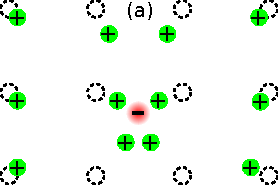
\includegraphics{metalcristal1}\hspace{4cm}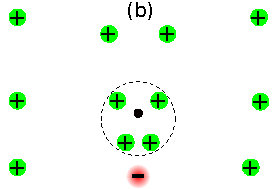
\includegraphics{metalcristal2}
  \caption{En la figura (a), los círculos con líneas a trazos representan las posiciones originales de los iones positivos en el cristal. Debido a la presencia del electrón de valencia, el cristal se polariza y se genera un exceso de carga positiva alrededor del electrón que resulta entonces apantallado. En la figura (b) se muestra como el exceso de carga positiva puede causar un efecto de atracción sobre otro electrón de valencia lo que permite la formación de un par de Cooper.}
  \label{fig:1}
\end{figure}

Este tipo de condensados de bosones, que ocurren por debajo de una cierta temperatura crítica, tiene todas las características de un éter lumínico: cuando la luz se propaga a través del condensado adquiere una masa emergente que hace que su velocidad sea menor que la velocidad límite de la relatividad especial. Esta nueva velocidad ya si depende de la velocidad del observador que la mida. Si se pudiese repetir el experimento de Michelson y Morley dentro de un superconductor: ¡daría un resultado positivo!

Pero, ¿cómo es posible que un fotón adquiera inercia?. Al tiempo en el que Clerk Maxwell estableció las ecuaciones del electromagnetismo, ya se conocía la Ley de Faraday que establece que los campos eléctricos en movimiento (las corrientes eléctricas) producen campos magnéticos. Usando principios de simetría, Maxwell completo las leyes electromagnéticas prediciendo que los campos magnéticos en movimiento producen también campos eléctricos. Como los campos eléctricos en movimiento producen campos magnéticos en movimiento, que a su vez producen de nuevo campos eléctricos en movimiento, entonces se genera un movimiento ondulatorio y las ecuaciones de Maxwell automáticamente predicen la existencia de ondas electromagnéticas. Una consecuencia inmediata es que la luz visible es simplemente un tipo especial de onda electromagnética en un rango de frecuencias determinado. Una onda electromagnética se puede representar entonces con un vector oscilante que representa el campo magnético, asociado con otro vector oscilante y perpendicular de campo eléctrico. La luz se propaga a la velocidad límite de la relatividad especial en una dirección perpendicular al plano definido por los dos vectores como se ilustra en la figura~\ref{fig:2}(a). Cuando la onda electromagnética se propaga dentro de un condensado sobre la superficie de un superconductor, una componente del par de Cooper se puede acoplar a los vectores magnético y eléctrico en la dirección de propagación de la onda, causando un efecto de frenado. En el lenguaje de la ruptura espontánea de simetría, que explica la formación del condensado por debajo de una temperatura crítica, se dice que fotón se come una componente del par de Cooper para así adquirir masa, como se muestra en la figura~\ref{fig:2}(b). Una vez la luz adquiere masa, las interacciones electromagnéticas se convierten en interacciones de rango finito. Es decir, que a partir de cierta separación entre las cargas eléctricas dentro de un superconductor, desaparecen las fuerzas eléctricas entre ellas. Aunque cuantitativamente estos efectos son pequeños pues la masa del fotón dentro de un superconductor es del orden de una billonésima de electron-voltio~\cite{beamline} (similar a las masas de neutrinos), cualitativamente el comportamiento cambia drásticamente: se pasa de una interacción de rango infinito mediada por fotones de masa cero, a una interacción de \emph{alcance restringido} mediada por fotones masivos. 

\begin{figure}
  \centering
  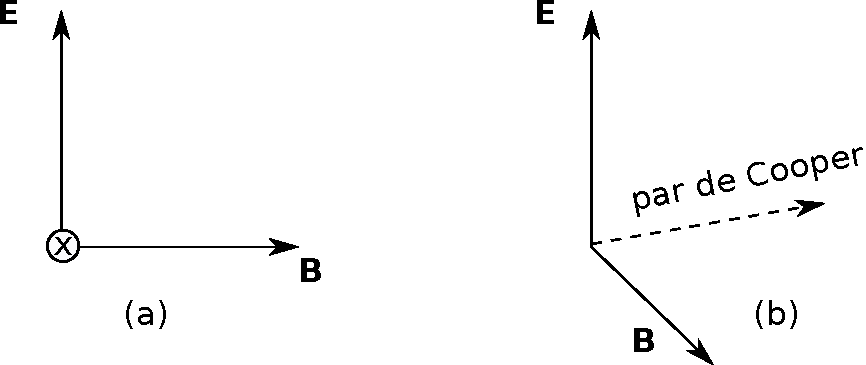
\includegraphics[scale=0.7]{ondaEM}
  \caption{En la figura (a), se representa los campos eléctricos y magnéticos de una onda electromagnética propagándose a la velocidad de la luz en una dirección entrando a la hoja. En  la figura (b) se muestra una onda electromagnética propagándose dentro de un condensado de pares de Cooper, en la dirección de la componente ilustrada del par de Cooper.}
  \label{fig:2}
\end{figure}


Cuando se calienta un superconductor metálico por encima de su temperatura crítica correspondiente a unos pocos grados kelvin sobre el cero absoluto, todo vuelve a la normalidad. El estado no superconductor es más simétrico porque los electrones del mar de Fermi están orientados en todas direcciones. El estado superconductor representa un estado menos simétrico pues todos los pares de Cooper están orientados formando un estado coherente en una dirección específica del espacio. Al formarse el condensado se da un fenómeno de \emph{ruptura espontánea de la simetría}: las simetrías iniciales que describen las interacciones del sistema se mantienen, pero el estado fundamental rompe la simetría.  

El electromagnetismo es la interacción mejor conocida de las cuatro interacciones fundamentales~\cite{pi}. Las interacciones fundamentales  entre partículas están mediadas por cierto conjunto de bosones.  Es así como la interacción electromagnética entre partículas cargadas, esta mediada por los fotones. Las interacción fuerte, que mantiene unidos de forma estable los componentes de los núcleos atómicos, está mediada por los gluones, los cuales tampoco requieren un medio para propagarse. La fuerza fuerte es en muchos otros aspectos similar a la fuerza electromagnética. 

Sin embargo, las interacciones débiles han resultados ser fuerzas de corto alcance, mediadas por nuevos fotones llamados $W$ y $Z$ que son bastante masivos: del orden de cien veces la masa del protón. La pregunta de si esas masas son reales o emergentes, se reduce a descubrir la existencia del éter a través del cual se propagan esas nuevas ondas débiles. Aunque no podemos acceder directamente a las componentes del condensado que se comen el $W$ y el $Z$ para adquirir masa, existe al menos otra componente del condensado que se debe materializar como partícula independiente y nueva: la partícula de Higgs. 

De confirmarse que la partícula recientemente descubierta en el Gran Acelerador de Hadrónes (LHC de sus siglas en inglés) corresponde al Higgs, significaría nada más y nada menos que el universo se encuentra en un estado de superconductividad débil (\emph{superconductividad electródebil para ser más exactos.}) El universo en su totalidad es un superconductor en el sentido de que las partículas que sólo tienen cargas débiles como los neutrinos, viajan por la materia sin mayor resistencia. De hecho nuestro cuerpo, e incluso el planeta entero, están siendo atravesados constantemente por neutrinos\footnote{Y por las supuestas partículas de materia oscura débilmente interactuantes, aunque estas aún no ha dejado trazas ni siquiera en los diversos experimentos de detección directa instalados en varios laboratorios subterráneos de la Tierra.}. Para hallar las excitaciones del éter débil, correspondientes a la partícula de Higgs, debemos calentar al menos una porción del universo por encima de la temperatura crítica de la ruptura espontánea de simetría electrodébil estimada en un cuadrillón de grados kelvin ($10^{15}\ $K). Eso es precisamente lo que se está haciendo el LHC en los puntos de colisión de los detectores ATLAS y CMS~\cite{quarknet}, de donde al parecer están emergiendo las primeras partículas de Higgs. 

 



\section{Campo escalar real}
Escribamos el Lagrangiano para una part\'\i cula escalar real de masa $m$ como
\begin{equation}
\label{eq:83qft}
\mathcal{L}=\tfrac{1}{2}\partial^\mu\phi\partial_\mu\phi-V(\phi)
\end{equation}
con
\begin{equation}
  V(\phi)=\tfrac{1}{2}\mu^2\phi^2.
\end{equation}
Este Lagrangiano es simétrico bajo la transformación discreta $\phi\to-\phi$. 

Cuando $\mu^2\gt 0$, el campo tiene excitaciones alrededor del mínimo del potencial que cuestan energía y dicho término se interpreta como la masa de la partícula. Ver figura \ref{fig:x2}. En Teoría Cuántica de Campos al estado de mínima energía se le llama el vacío y las excitaciones alrededor del vació corresponden a las partículas.
%noinstiki
\begin{figure} %noinstiki
  \centering %noinstiki
  
\includegraphics[scale=0.8]{vphi2}
  \caption{$V(\phi)=\frac{1}{2}\mu^2 \phi^2$ con $\mu^2\gt 0$} %noinstiki
  \label{fig:x2} %noinstiki
\end{figure} %noinstiki <div id="fig:x2">Figura: Un mínimo</div>
%noinstiki![cuerda](http://gfif.udea.edu.co/figfs/vphi2.png)
%noinstiki

Si $\mu^2\lt 0$, no existe un mínimo del potencial alrededor del cual el campo pueda oscilar. Además el alejamiento del campo del punto de simetría del potencial no cuesta energía. Por consiguiente en ese caso, el término de interacción
\begin{equation}
  V(\phi)=\tfrac{1}{2}\mu^2   \qquad 
  \mu^2\lt 0,
\end{equation}
no puede interpretarse como un término de masa en el Lagrangiano dado por la ec.~\eqref{eq:83qft}. 

Consideremos ahora el potencial
\begin{equation}
  V(\phi)=\tfrac{1}{2}\mu^2\phi^2+\tfrac{1}{4}\lambda\phi^4
  \qquad   \mu^2\lt 0,\ \lambda\gt 0
\end{equation}
que mantiene la simetría bajo la transformación discreta $\phi\to-\phi$. $\lambda\gt 0$ garantiza la aparición de los dos mínimos que se muestran el la figura \ref{fig:x2l}. Si la energía es suficientemente alta como se muestra en la figura~\ref{fig:x2l}, las excitaciones son simétricas con respecto al máximo del potencial y el término en $\mu^2$ no puede interpretarse como masa para la partícula escalar. 

%noinstiki
\begin{figure} %noinstiki
  \centering %noinstiki
  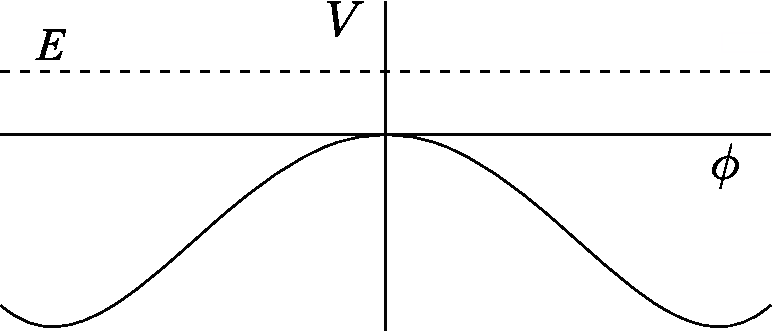
\includegraphics{vphi4}
  \caption{$V(\phi)=\frac{1}{2}\mu^2 \phi^2+\frac{1}{4}\lambda\phi^4$ con $\mu^2\lt 0$, y $\lambda\gt 0$. Simetría exácta} %noinstiki
  \label{fig:x2l} %noinstiki
\end{figure} %noinstiki <div id="fig:x2l">Figura: Mínimos degenerados</div>
%noinstiki![cuerda](http://gfif.udea.edu.co/figfs/vphi4.png)
%noinstiki
Sin embargo, si la energía es suficientemente baja como se muestra en la figura~\ref{fig:x2lm}, las excitaciones alrededor del mínimo dan lugar a la aparición de un término de masa para el campo escalar. Además, dichas excitaciones no respetan la simetrías $\phi\to-\phi$. En tal caso decimos que la simetría ha sido espontáneamente rota: aunque el Lagrangiano mantiene la simetría original, el vacío la rompe. 

%noinstiki
\begin{figure} %noinstiki
  \centering %noinstiki
  %noinstiki
  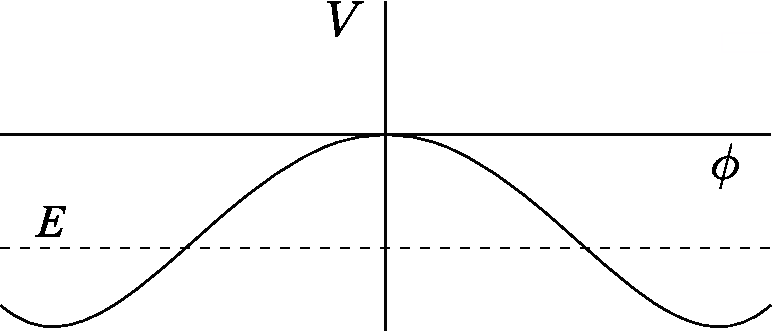
\includegraphics{vphi4m}
  \caption{$V(\phi)=\frac{1}{2}\mu^2 \phi^2+\frac{1}{4}\lambda\phi^4$ con $\mu^2\lt 0$, y $\lambda\gt 0$. Simetría espontáneamente rota.} %noinstiki
  \label{fig:x2lm} %noinstiki
\end{figure}  %noinstiki <div id="fig:x2lm">Figura: Simetría espontáneamente rota  </div>
%noinstiki![vphi4lm](http://gfif.udea.edu.co/figfs/vphi4lm.png)
%noinstiki

Para analizar cuantitativamente el espectro de partículas es necesario expandir el campo alrededor del mínimo y determinar las excitaciones. Establezcamos en primer lugar los mínimos del potencial. La $\partial V/\partial\phi=0$ da lugar a
\begin{align}
  \mu^2\phi+\lambda\phi^3&=0\\
  \phi(\mu^2+\lambda\phi^2)&=0,
\end{align}
con extremos $\phi_{\text{max}}=0$, y 
\begin{equation}
  \label{eq:90qft}
  \phi_{\text{min}}\equiv\langle\phi\rangle\equiv v=\pm\sqrt{\frac{-\mu^2}{\lambda}}.
\end{equation}
De hecho 
\begin{equation}
  \frac{\partial^2V}{\partial\phi^2}=\mu^2+3\lambda\phi^2.
\end{equation}
$\phi=0$ corresponde a un máximo, mientras que la segunda derivada para $\phi=\pm\sqrt{-\mu^2/\lambda}$ es $-2\mu^2\gt 0$ y corresponden a los mínimos. Expandiendo el campo alrededor del mínimo
\begin{equation}
  \phi(x)=H(x)+v
\end{equation}
\begin{align}
  V(\phi)=&\tfrac{1}{2}\mu^2 \phi^2+\tfrac{1}{4}\lambda\phi^4\nonumber\\
  =&\tfrac{1}{2}\mu^2 (H+v)^2+\tfrac{1}{4}\lambda(H+v)^4\nonumber\\
  =&\tfrac{1}{2}\mu^2 (H+v)^2+\tfrac{1}{4}\lambda(H+v)^4\nonumber\\
  =&\tfrac{1}{2}\mu^2 \left(H^2+2vH+v^2\right)+\tfrac{1}{4}\lambda\left(H^2+2vH+v^2\right)^2\nonumber\\
  =&\tfrac{1}{2}\mu^2 \left(H^2+2vH+v^2\right)+\tfrac{1}{4}\lambda\left[H^4+2H^2\left(2vH+v^2\right)+\left(2vH+v^2\right)^2\right]\nonumber\\
  =&\tfrac{1}{2}\mu^2 \left(H^2+2vH+v^2\right)+\tfrac{1}{4}\lambda\left[H^4+4vH^3+2H^2v^2+4v^2H^2+4v^3H+v^4\right]\nonumber\\
  =&\tfrac{1}{2}\mu^2 \left(H^2+2vH+v^2\right)+\tfrac{1}{4}\lambda\left[H^4+4vH^3+6H^2v^2+4v^3H+v^4\right]\nonumber\\
  =&\tfrac{1}{2}\mu^2H^2-\tfrac{3}{2}H^2\mu^2+\mu^2vH-\mu^2vH+\tfrac{1}{2}\mu^2v^2-\tfrac{1}{4}\mu^2v^2+\tfrac{1}{4}\lambda\left[H^4+4vH^3\right]\nonumber\\
\label{eq:84qft}
V(H)=&\tfrac{1}{2}\left(-2\mu^2\right)H^2+\lambda vH^3+\tfrac{1}{4}\lambda H^4+\tfrac{1}{4}\mu^2v^2,
\end{align}
y
\begin{equation}
  \label{eq:88qft}
  \mathcal{L}_H=\tfrac{1}{2}\partial^\mu H\partial_\mu H-\tfrac{1}{2}\left(-2\mu^2\right)H^2-\lambda vH^3-\tfrac{1}{4}\lambda H^4+\text{constant}.
\end{equation}
Entonces $H$ adquiere una masa $-2\mu^2$ y no es invariante bajo $H\to-H$. 

Otro método es usar las ecuaciones de mínimo $-\mu^2=\lambda v^2$, para eliminar un parámetro del potencial:
\begin{align}
  V(\phi)&=-\tfrac{1}{2}\lambda v^2\phi^2+\tfrac{1}{4}\lambda\phi^4\nonumber\\
  =&-\tfrac{1}{2}\lambda v^2 \left(H^2+2vH+v^2\right)+\tfrac{1}{4}\lambda\left[H^4+4vH^3+6H^2v^2+4v^3H+v^4\right]\nonumber\\
  =&\lambda v^2H^2+\lambda vH^3+\tfrac{1}{4}\lambda H^4+\text{constant}.
\end{align}
Podemos escribir el potencial en términos del  nuevo campo como
\begin{align}
\label{eq:higgspot}
  V(H)=\frac{1}{2}m_H^2H^2+\frac{1}{2}\frac{m_H^2}{v}H^3+\frac{1}{8}\frac{m_H^2}{v^2} H^4\,.
\end{align}
donde
\begin{equation}
\label{eq:higgsmass}
  m_H^2=2\left|\mu^2\right|=2\lambda v^2
\end{equation}

\subsection{Ausencia de taquiones}

Uno se podría preocupar por la presencia de un término de masa
imaginaria en el Lagrangiano, pero como estamos hablando de
transiciones de fase, estos porcesos deben suceder en presencia de
temperatura, por ejemplo la temperatura asociada al universo primitivo
durante las fases tempranas del Big Bang. En presencia de temperatura,
todas las partículas adquieren una masa térmica proporcional a la
temperatura como resultado de su interacción con el plasma. De este
modo, a altas temperaturas la masa de la partícula escalar esta
dominada por la temperatura y al ser positiva el potencial escalar
tiene un único mínimo simétrico. Cuando la temperatura baja lo
suficiente para que la masa al cuadrado negativa domine, el mínimo se
convierte en un máximo local altamente inestable y ocurre muy
rapidamente la transición de fase al nuevo mínimo no simétrico donde
la masa del escalar esta bien definida.

\subsection{Caso complejo}


Consideremos ahora un campo escalar complejo sin término de masa, pero con potencial:
\begin{equation}
  \label{eq:85qft}
  \mathcal{L}=\partial^\mu\phi^*\partial_\mu\phi-V(\phi)
\end{equation}
\begin{equation}
  V(\phi)=\mu^2\phi^*\phi+\lambda(\phi^*\phi)^2 
  \qquad 
  \mu^2\lt 0,\ \lambda\gt 0 
\end{equation}
La simetría del Lagrangiano corresponde a $U(1)$ global. Este potencial corresponde al ``sombrero mexicano'', como se ilustra en la Figura \ref{fig:mexicanhat}. Para una energía suficientemente baja de manera que el campo deba oscilar alrededor del mínimo aparecen dos tipos de excitaciones. Una sobre las paredes  que cuestan energía y corresponden a un campo escalar masivo como en el caso anterior, y otra a lo largo de la circunferencia de mínimo, que corresponde a una partícula escalar sin masa, y es llamada bosón del Golstone. 



\begin{figure}
  \centering
  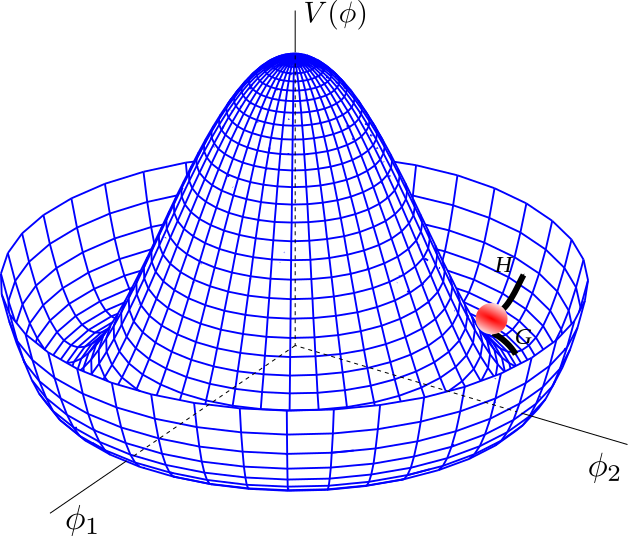
\includegraphics[scale=0.5]{mexicanhat}
  \caption{Potential for complex scalar field}
  \label{fig:mexicanhat}
\end{figure}



El Lagrangiano escalar complejo es equivalente al Lagragiano de dos campos escalares reales con los mismos paramétros. Para un conjunto de $N$ campos reales tenedremos (suma sobre $i$) \cite{Peskin}\footnote{\S 11.1}: 
\begin{align}
  \mathcal{L}=\frac{1}{2}\partial^\mu\phi^i\partial_\mu\phi_i-\frac{1}{2}\mu^2\phi_i\phi^i-\frac{1}{2}\mu^2\left(\phi_i\phi^i\right)^2\,,
\end{align}
que es invariante bajo una simetría $O(N)$
\begin{align}
  \phi^i\to{\phi'}^i=R^{ij}\phi^j\,,
\end{align}
para cualquier matriz $N\times  N$ ortogonal $R$. El análisis para $N=2$ da lugar a un bosón de Goldstone. El anális para $N>2$ es el mismo y por cada campo real que se introduzca aparece un nuevo bosón de Goldstone \cite{Peskin}:
\begin{quote}
  [\ldots] there are not continuous symmetries for $N=1$, while for $N=2$ there is a single direction of rotation. A rotation in $N$ dimensions can be in any one of $N(N-1)$ planes, so the $O(N)$--symmetric theory has $N(N-1)/2$ continuous symmetries. After spontaneous symmetry breaking there are $(N-1)(N-2)/2$  remaining symmetries corresponding to rotations of the $(N-1)$ [non massive] fields. The number of \emph{broken} symmetries is the difference, $N-1$.
\end{quote}
Entonces tenemos el siguiente teorema \cite{Peskin}
\begin{quote}
\emph{Goldstone's theorem states that for every spontaneously broken continuous symmetry, the theory must contain a massless particle.}
\end{quote}

Also from \cite{Peskin}\footnote{Introduction to Chapter 20}
\begin{quote}
  In a global symmetry  that is spontaneously broken the symmetry currents are still conserved and interactions are similarly restricted [the Lagrangian keeps the symmetry], but the vacuum state does not respect the symmetry and the particles do not form obvious symmetry multiplets. Instead, such a theory contains massless particles, Goldstone bosons, one for each generator of the spontaneously broken symmetry. The third case is that of a local, or gauge, symmetry. [\ldots] such a symmetry requires the existence of a massless vector field for each symmetry generator, and the interactions among these fields are highly restricted.

It is now only natural to consider a fourth possibility: What happens if we include both local gauge invariance  and spontaneous symmetry breaking in the same theory?
\end{quote}
 
\section{Principio gauge local}



En el caso de la Acción invariante gauge local bajo el Grupo $U(1)$, tenemos el Lagrangiano 
\begin{equation}
  \label{eq:89qft}
  \mathcal{L}=\left(\mathcal{D}^\mu\phi\right)^*\mathcal{D}_\mu\phi-\mu^2\phi^*\phi-\lambda\left(\phi^*\phi\right)^2-\tfrac{1}{4}F^{\mu\nu}F_{\mu\nu}
  \qquad 
  \mu^2\lt 0\text{ and } \lambda\gt 0\,.
\end{equation}
donde
\begin{align}
  \mathcal{D}_{\mu}=\partial_{\mu}+iq A_{\mu}\,.
\end{align}

Este es el Lagrangiano más general posible para un campo escalar complejo y el campo $A_\mu$ que deja la Acción invariante de Lorentz e invariante bajo la transformación gauge $U(1)$
\begin{align}
\label{eq:sqedgu}
  \phi(x)\to \phi'(x)=e^{i\theta(x)} \phi(x)\,,
\end{align}
En el caso de la superconductividad  electromagnético, $\phi$ representaría al campo escalar asociado al par de Cooper con carga eléctrica $-2$. Claramente el Lagrangiana en la ec.~\eqref{eq:89qft} es invariante local bajo tal $U(1)$ de carga eléctrica. 


\subsection{Gauge unitario}
Como $\phi$ es un campo complejo, podemos escribirlo en coordenadas polares con un campo real asociado a la magnitud del campo complejo y otro a la fase
\begin{align*}
  \phi(x)=\varphi(x)e^{i\eta(x)}
\end{align*}
Expandiendo el campo $\varphi(x)$ alrededor del mínimo: $\varphi(x)=(H(x)+v)/\sqrt{2}$, tenemos
\begin{align*}
    \phi(x)=e^{i\eta(x)}\left(\frac{H(x)+v}{\sqrt{2}}\right)\,.
\end{align*}


La libertad gauge nos permite en un momento determinado escoger la fase $\theta(x)$ de la ec.~\eqref{eq:sqedgu} sin que ese alteren los observables de la teoría. Para el campo en coordenadas polares tenemos que
\begin{align*}
     \phi\to\phi'=e^{i\theta(x)}e^{i\eta(x)}\left(\frac{H(x)+v}{\sqrt{2}}\right)
\end{align*}
Haciendo $\theta(x)=-\eta(x)$,
\begin{align}
\label{eq:87qft}
   \phi\to\phi'=&e^{-i\eta(x)+i\eta(x)}\left(\frac{H(x)+v}{\sqrt{2}}\right)=\frac{H(x)+v}{\sqrt{2}} \nonumber\\
   A_{\mu}\to A_{\mu}'=&A_{\mu}-\frac{1}{q}\partial_{\mu}\theta(x)\,.
\end{align}
\begin{align}
  \mathcal{L}\to\mathcal{L}' &=\left[\left(\mathcal{D}^\mu\right)'\phi'\right]^*\left(\mathcal{D}_\mu\right)'\phi'-\mu^2\left(\phi^*\right)'\phi'-\lambda\left[\left(\phi^*\right)'\phi'\right]^2-\tfrac{1}{4}\left(F^{\mu\nu}F_{\mu\nu}\right)'\nonumber\\
 &=\tfrac{1}{2}\left[\partial^\mu H+ig{A'}^\mu(H+v)\right]\left[\partial_\mu H-ig{A'}_\mu(H+v)\right]-\tfrac{1}{2}\mu^2(H+v)^2-\tfrac{1}{4}\lambda(H+v)^4-\tfrac{1}{4}\left(F^{\mu\nu}F_{\mu\nu}\right)'\,.
\end{align}

En adelante omitiremos las primas, aunque debe estar claro que se esta trabajando en el gauge específico de la ec.~\eqref{eq:87qft}. Entonces
\begin{align}
  \mathcal{L}&=\tfrac{1}{2}\partial^\mu H\partial_\mu H-\tfrac{1}{2}\mu^2(H+v)^2-
  \tfrac{1}{4}\lambda(H+v)^4+\tfrac{1}{2}g^2A^\mu A_\mu(H+v)^2
  -\tfrac{1}{4}F^{\mu\nu}F_{\mu\nu}.
\end{align}
Usando la ec.~\eqref{eq:84qft}
\begin{equation}
  \label{eq:94qft}
  \mathcal{L}=\mathcal{L}_H+\mathcal{L}_{A^\mu}+\tfrac{1}{2}g^2A^\mu A_\mu H^2+g^2vA^\mu A_\mu H,
\end{equation}
donde $\mathcal{L}_H$ esta dado por la ec.~\eqref{eq:88qft} y
\begin{equation}
  \mathcal{L}_{A^\mu}=-\tfrac{1}{4}F^{\mu\nu}F_{\mu\nu}+\tfrac{1}{2}g^2v^2A^\mu A_\mu.
\end{equation}
Teniendo en cuenta la ec.~\eqref{eq:23qft} para el Lagrangiano de Proca, vemos que como consecuencia de la ruptura espontánea de simetría el campo gauge ha adquirido una masa
\begin{equation}
  m_{A^\mu}=gv.
\end{equation}

El mecanismo completo mediante el cual, a partir de un Lagrangiano invariante gauge local, los bosones gauge adquieren masa se llama \emph{mecanismo de Brout–Englert–Higgs} \cite{Englert:1964et,Higgs:1964pj}. La partícula escalar que adquiere masa se llama Higgs, mientras que el bosón de Goldstone es absorbido por campo gauge como modo longitudinal. 

El número de grados de libertad independientes en el Lagrangiano original en la ec.~\eqref{eq:89qft} es cuatro. Correspondientes a los dos grados de libertad del bosón gauge no masivo y los dos del campo escalar complejo. En el Lagrangiano final en la ec.~\eqref{eq:94qft} no aparece el bosón de Goldstone. Sin embargo esto no es un problema porque dicho Lagrangiano también tiene cuatro grados de libertad correspondientes a  los tres grados de libertad del bosón gauge masivo y al grado de libertad del bosón de Higgs. 



\subsection{Superconductivity}

El campo $H$ dentro del superconductor, que hereda la carga $-2$ de
$\phi$, rompe espontáneamente carga eléctrica para esa configuración
especial del vacío (mínimo de energía) donde se forma el condensado de
pares de Cooper. Pero el la acción claramente conserva en todo momento
la carga eléctrica.

A review ot the use of the Proca Equations for a massive photon in superconductivity is given in~\cite{massivephoton}. A popularization review along this lines is in the book of Frank Wilczek ``The Lightness of Being'' (see Additional references).

The photon mass inside a superconductor is $10^{-11}\,$GeV (or 1/1000 of the electron mass according to~\cite{massivephoton}). Also from the article in Beamline $\lambda\sim 10\ \mu\text{m}$ y $M_\gamma=\hbar/\lambda c$ %check numbers

There are two important length scales in a superconductor. The first measures how efficientrly the condensate expels a magnetic field. In fact, the expulsion is not 

Additional references:
\begin{itemize}
\item The Lightness of Being: Mass, Ether, and the Unification of Forces,
Frank Wilczek, \url{http://www.amazon.com/The-Lightness-Being-Unification-Forces/dp/0465018955}
\item \url{http://www.scholarpedia.org/article/Englert-Brout-Higgs-Guralnik-Hagen-Kibble_mechanism_(history)}
\item Elementary Particle Physics: Volume 1: Quantum Field Theory and ..., Volume 1
 By Yorikiyo Nagashima, \url{Elementary Particle Physics: Volume 1: Quantum Field Theory and ..., Volume 1
 By Yorikiyo Nagashima}
\item From Superconductors 
to Supercolliders
by LANCE DIXON \url{http://www.slac.stanford.edu/pubs/beamline/26/1/26-1-dixon.pdf}
\item Electrodynamics of Superconductors \url{http://www.physics.buffalo.edu/phy514/w11/index.html}
\item Observan el análogo a un bosón de Higgs en un superconductor \url{http://francis.naukas.com/2014/09/05/analogo-al-boson-de-higgs-en-un-superconductor/}
\end{itemize}


%\left(\right)
%%% Local Variables: 
%%% mode: latex
%%% TeX-master: "fullnotes"
%%% ispell-local-dictionary: "castellano8"
%%% End:}
\mode<presentation>{%instiki:category: FisicaSubatomica

\chapter{Fermiones}
\label{cha:fermiones}
%instiki:
%instiki:***
%instiki:
%instiki:[[NotasFS|Tabla de Contenidos]]
%instiki:
%instiki:***
%instiki:
%instiki:* [Ecuaci\'on de Dirac](#ecuacion-de-dirac)
%instiki:
%instiki:* [Electrodin\'amica Cu\'antica](#electr-cuant)
%instiki:
%instiki:* [Cromodin\'amica Cu\'antica](#inter-fuert)
%instiki:
%instiki:* [Soluci\'on de part\'\i cula libre](#solucion-de-parti)
%instiki:
%instiki:***
%instiki:



\section{Fermiones quirales de cuatro componentes}
\label{sec:ferm-quir-de}

Sea
\begin{align}
  P_L\equiv&\frac{1-\gamma_5}{2}\nonumber\\
  P_R\equiv&\frac{1+\gamma_5}{2}\,.
\end{align}
Además
\begin{align}
  \psi_L\equiv P_L\psi\nonumber\\
  \psi_R\equiv P_R\psi\,.
\end{align}
Entonces
\begin{align}
  \psi=\psi_L+\psi_R\,.
\end{align}

Las matrices $P_{L,R}$ tienen las propiedades
\begin{align}
  P_L+P_R&=1 & P_{L,R}^2&=P_{L,R}P_{L,R}=P_{L,R}\nonumber\\
  P_L P_R&=0& P_{L,R}^\dagger&=P_{L,R}\,.
\end{align}
Usando la ec.~(\ref{eq:218qft})
\begin{align}
  P_{L,R}\gamma^\mu=\frac{1\mp\gamma_5}{2}\gamma^\mu=\gamma^\mu\frac{1\pm\gamma_5}{2}=\gamma^\mu P_{R,L}
\end{align}
Para escribir el Lagrangiano en término de los nuevos $\psi_{L,R}$ debemos tener en cuenta que
\begin{align}
  \overline{\psi_{L,R}}=(P_{L,R}\psi)^\dagger\gamma^0=\psi^\dagger P_{L,R}\gamma^0=\psi^\dagger\gamma^0P_{R,L}=\overline{\psi}P_{R,L}
\end{align}
\begin{align}
  \label{eq:221qft}
  \mathcal{L}=&i\overline{\psi}\gamma^\mu\partial_\mu\psi-m\overline{\psi}\psi\nonumber\\
  =&i\overline{\psi}(P_L+P_R)\gamma^\mu\partial_\mu\psi-m\overline{\psi}(P_L+P_R)\psi\nonumber\\
  =&i\overline{\psi}P_L\gamma^\mu\partial_\mu\psi+i\overline{\psi}P_R\gamma^\mu\partial_\mu\psi-m\overline{\psi}P_L\psi-m\overline{\psi}P_R\psi\nonumber\\
  =&i\overline{\psi}P_L P_L\gamma^\mu\partial_\mu\psi+i\overline{\psi}P_R P_R\gamma^\mu\partial_\mu\psi-m\overline{\psi}P_L P_L\psi-m\overline{\psi}P_R P_R\psi\nonumber\\
  =&i\overline{\psi}P_L\gamma^\mu\partial_\mu P_R\psi+i\overline{\psi}P_R\gamma^\mu\partial_\mu P_L\psi-m\overline{\psi}P_L P_L\psi-m\overline{\psi}P_R P_R\psi\nonumber\\
  =&i\overline{\psi_R}\gamma^\mu\partial_\mu\psi_R+i\overline{\psi_L}\gamma^\mu\partial_\mu\psi_L-m(\overline{\psi_R}\psi_L+\overline{\psi_L}\psi_R)\,.
\end{align}
En términos de espinores izquierdos y derechos de cuatro componentes la transformación de paridad 
\begin{align}
  \label{eq:220qft}
  t&\to t&\mathbf{x}&\to -\mathbf{x}&\psi_L(t,\mathbf{x})\to&\psi_R(t,-\mathbf{x}),& \psi_R(t,\mathbf{x})&\to\psi_L(t,-\mathbf{x})\nonumber\\
  \partial_0&\to \partial_0&\boldsymbol{\nabla}&\to -\boldsymbol{\nabla}&\psi_L(t,\mathbf{x})\to&\psi_R(t,-\mathbf{x}),& \psi_R(t,\mathbf{x})&\to\psi_L(t,-\mathbf{x})\,.
\end{align}
Además $\mathbf{L}=\mathbf{r}\times \mathbf{p}\to(-\mathbf{r})\times (-\mathbf{p})=\mathbf{L}$, y como $\gamma^\mu$ esta asociado al momento angular intrínsico, entonces también $\gamma^\mu\to\gamma^\mu$


Entonces la transformación de paridad da lugar a (sin tener en cuenta el cambio de argumento en los campos que desaparece en la integral de la Acción)
\begin{align}
  \overline{\psi_R}\gamma^\mu\partial_\mu\psi_R=\overline{\psi_R}\gamma^0\partial_0\psi_R+\overline{\psi_R}\boldsymbol{\gamma}\cdot\boldsymbol{\nabla}\psi_R 
\to&\overline{\psi_L}\gamma^0\partial_0\psi_L-\overline{\psi_L}\boldsymbol{\gamma}\cdot\boldsymbol{\nabla}\psi_L\nonumber\\
=&\overline{\psi_L}\gamma^0\partial_0\psi_L+\overline{\psi_L}\boldsymbol{\gamma}^\dagger\cdot\boldsymbol{\nabla}\psi_L\nonumber\\
=&\overline{\psi_L}\gamma^0\gamma^0\gamma^0\partial_0\psi_L+\overline{\psi_L}\gamma^0\boldsymbol{\gamma}\gamma^0\cdot\boldsymbol{\nabla}\psi_L\nonumber\\
=&\overline{\psi_L}\tilde\gamma^0\partial_0\psi_L+\overline{\psi_L}\tilde{\boldsymbol{\gamma}}\cdot\boldsymbol{\nabla}\psi_L\nonumber\\
=&\overline{\psi_L}\tilde\gamma^\mu\partial_\mu\psi_L\,.
\end{align}
Entonces
\begin{align}
   \mathcal{L}\to\mathcal{L}'=&i\overline{\psi_R}\tilde\gamma^\mu\partial_\mu\psi_R+i\overline{\psi_L}\tilde\gamma^\mu\partial_\mu\psi_L-m(\overline{\psi_R}\psi_L+\overline{\psi_L}\psi_R)\,,
\end{align}
donde $\tilde\gamma^\mu=U\gamma^\mu U^\dagger$, con $U=\gamma^0$. Como las dos representaciones dan lugar a la misma física, podemos decir que la Acción en términos de espinores $L,R$ de cuatro componentes es invariante bajo la transformación de paridad.

La existencia de ambos espinores $\psi_{L,R}$ garantizan que el Lagrangiano de Dirac es invariante bajo la transformación de paridad. 

La corriente de la electrodinámica cuántica en ec.~\eqref{eq:222qft} (o la de la cromodinámica cuántica, ec.~\eqref{eq:223qft}) conservan paridad ya que, siguiendo los mismos pasos que en la ec.~\eqref{eq:221qft}
\begin{align}
  \label{eq:224qft}
  \overline{\psi}\gamma^\mu\psi=\overline{\psi_L}\gamma^\mu\psi_L+\overline{\psi_R}\gamma^\mu\psi_R\to\overline{\psi_L}\tilde{\gamma}^\mu\psi_L+\overline{\psi_R}\tilde{\gamma}^\mu\psi_R\,.
\end{align}
Si para alguna partícula, como es el caso del neutrino, no existe la componente derecha, entonces la correspondiente interacción vectorial viola paridad y no puede tener ni interacciones electromagnéticas ni fuertes, es decir, no se acopla con el fotón o los gluones. Además dicha partícula no puede tener masa de Dirac. En el caso del neutrino esto se entiende pues al no tener carga eléctrica sólo requiere dos grados de libertad independientes.

De otro lado, si una determinada interacción, como es el caso de la interacción débil, solo participa la componente izquierda de la ec.~\eqref{eq:224qft}, está corresponde a una interacción del tipo
\begin{align}
  \overline{\psi}_L\gamma^\mu\psi_L&=\overline{\psi}P_R\gamma^\mu P_L\psi=\overline{\psi}\gamma^\mu P_L\psi\nonumber\\
  &=\overline{\psi}\gamma^\mu\left(\frac{1-\gamma_5}{2}\right)\psi\nonumber\\
  &=\tfrac{1}{2}\overline{\psi}\left(\gamma^\mu-\gamma^\mu\gamma_5\right)\psi\,,
\end{align}
que de acuerdo a la asignación en la Tabla corresponde a una corriente V--A. 

\subsection{Fermiones de Weyl}
\label{sec:fermiones-de-weyl}
%Weyl because $\psi^\dagger$ instead $\bar \psi$
Sea $\psi$ un campo que satisface una ecuaci\'on covariante de segundo orden. La parte cin\'etica del Lagrangiano sin t\'erminos de masa y sin t\'erminos de interacci\'on debe tener la forma 
\begin{equation}
\label{eq:98}
  \mathcal{L}=\frac{i}{2}\psi^\dagger a^\mu\partial_\mu\psi-\frac{i}{2}\partial_\mu\psi^\dagger {a^\mu}^\dagger\psi-m\psi^\dagger b\psi
\end{equation}
La Acci\'on debe ser real, de modo que el Lagrangiano tambi\'en. En efecto
\begin{align*}
  \mathcal{L}^\dagger&=\left(\frac{i}{2}\psi^\dagger a^\mu\partial_\mu\psi-\frac{i}{2}\partial_\mu\psi^\dagger {a^\mu}^\dagger\psi\right)^\dagger-m\psi^\dagger b^\dagger \psi\\
  &=\left(-\frac{i}{2}\partial^\mu\psi^\dagger a_\mu^\dagger \psi+\frac{i}{2}\psi^\dagger {a^\mu} \partial_\mu\psi\right)-m\psi^\dagger b^\dagger \psi\\
  &=\mathcal{L} \qquad \text{si }b^\dagger = b\,.
\end{align*}
Como al aplicar las ecuaciones de Euler-Lagrange a este Lagrangiano debemos obtener la ecuaci\'on de Scrh\"odinger
\begin{align}
i\frac{\partial}{\partial t}\psi=\widehat{H}\psi
\end{align}
con $\widehat{H}$ una funci\'on por determinar del operador $\hat{\mathbf{p}}$, entonces
\begin{align}
  a_\mu^\dagger=a_\mu
\end{align}

El Lagrangiano en ec.~(\ref{eq:98}) puede reescribirse como
\begin{align}
  \label{eq:197}
  \mathcal{L}&=\frac{i}{2}\psi^\dagger a^\mu\partial_\mu\psi-\frac{i}{2}\partial_\mu\left(\psi^\dagger a^\mu\psi\right)+\frac{i}{2}\psi^\dagger a^\mu\partial_\mu\psi-m\psi^\dagger b\psi\nonumber\\
  &=i \psi^\dagger a^\mu\partial_\mu\psi-\frac{i}{2}\partial_\mu\left(\psi^\dagger a^\mu\psi\right)-m\psi^\dagger b\psi\nonumber\\
  \mathcal{L}&=i \psi^\dagger a^\mu\partial_\mu\psi-m\psi^\dagger b\psi
\end{align}

Ahora utilizaremos el m\'etodo desarrollado en cap\'\i tulos anteriores para analizar el Lagrangiano. Calcularemos las ecuaciones de Euler-Lagrange, la corriente conservada y el tensor de momento-energ\'\i a.


\section{Soluciones a la ecuaci\'on de Dirac}
\label{sec:soluc-la-ecuac}

\subsection{Lagrangiano de Weyl}
\label{sec:lagrangiano-de-weyl}


En la ec.~\eqref{eq:118}, obtuvimos el Hamiltoniano en ec.~\eqref{eq:103}
\begin{equation}
  \hat{H}= \gamma_0(\boldsymbol{\gamma}\cdot\mathbf{p}+m)=\boldsymbol{\alpha}\cdot\mathbf{p}+\beta m\,.
\end{equation}
Una escogencia particular de las cuatro matrices $\gamma^\mu$, conocida como la representaci\'on de Weyl, o representaci\'on quiral, puede escribirse en t\'erminos de la matrices de Pauli. Escritas en bloques $2\times2$, tenemos
\begin{equation}
  \gamma^0=
  \begin{pmatrix}
    0&\sigma_0\\
    \sigma_0&0
  \end{pmatrix}\qquad
  \gamma_i=\begin{pmatrix}
    0&\sigma_i\\
    -\sigma_i&0
  \end{pmatrix}.
\end{equation}
Con $\sigma^0=1$. Con la matriz de tranformaci\'on
\begin{equation}
  U=\frac{1}{\sqrt{2}}
  \begin{pmatrix}
    1&1\\
    -1&1    
  \end{pmatrix}
\end{equation}
podemos obtener la representaci\'on de Dirac, tal que $U$ diagonaliza $\gamma^0$,
\begin{equation}
  \gamma^0=
  \begin{pmatrix}
    \sigma^0&0\\
    0&-\sigma^0
  \end{pmatrix}\qquad
  \gamma_i=\begin{pmatrix}
    0&\sigma_i\\
    -\sigma_i&0
  \end{pmatrix}.
\end{equation}
En adelante trabajaremos en la representaci\'on de Weyl que en forma compacta es
\begin{equation}
  \gamma^\mu=\begin{pmatrix}
    0&\sigma^\mu\\
    \bar{\sigma}^\mu & 0
  \end{pmatrix}
\end{equation}
donde
\begin{align}
  \sigma^\mu&=(\sigma^0,\sigma^1,\sigma^2,\sigma^3)\nonumber\\
  \bar{\sigma}^\mu&=(\sigma^0,-\sigma^1,-\sigma^2,-\sigma^3)\nonumber\\
\end{align}
Hemos escrito las matrices de Dirac en bloques $2\times2$, y es natural escribir similarmente las cuatro componentes del campo de Dirac como un par de campos de dos componentes
\begin{align}
  \psi=  \begin{pmatrix}
    \psi_L\\
    \psi_R    
  \end{pmatrix}=\begin{pmatrix}
    \psi_L\\
    0   
  \end{pmatrix}+\begin{pmatrix}
    0\\
    \psi_R    
  \end{pmatrix}
\end{align}
Donde $\psi_{L,R}$ son espinores de Weyl de dos componentes. En la representaci\'on de Weyl el Lagrangiano se puede escribir como
\begin{align}
\label{eq:200}
  \mathcal{L}=&i\bar{\psi}\gamma^\mu\partial_\mu\psi-m\bar{\psi}\psi\nonumber\\
  =&i\psi^\dagger \gamma^0\gamma^\mu\partial_\mu\psi-m\psi^\dagger \gamma^0 \psi\nonumber\\
  =&i\psi^\dagger  \begin{pmatrix}
    0 & 1\\
    1&0
  \end{pmatrix}
  \begin{pmatrix}
    0 &\sigma^\mu \\
    \bar{\sigma}^\mu&0
  \end{pmatrix}\partial_\mu\psi-m\psi^\dagger
  \begin{pmatrix}
    0 & 1\\
    1&0
  \end{pmatrix}\psi\nonumber\\
=&i\begin{pmatrix}
 \psi_L^\dagger & \psi_R^\dagger
\end{pmatrix}
 \begin{pmatrix}
   \bar{\sigma}^\mu &0\\
   0&\sigma^\mu
 \end{pmatrix} \begin{pmatrix}
   \partial_\mu\psi_L\\
   \partial_\mu\psi_R
 \end{pmatrix}-m
 \begin{pmatrix}
   \psi_L^\dagger&\psi_R^\dagger
 \end{pmatrix}
 \begin{pmatrix}
   0&1\\
   1&0
 \end{pmatrix}
 \begin{pmatrix}
   \psi_L\\ \psi_R
 \end{pmatrix}\nonumber\\
 =& i\psi_L^\dagger \bar{\sigma}^\mu\partial_\mu\psi_L+i\psi_R^\dagger \sigma^\mu\partial_\mu\psi_R
  -m(\psi_L^\dagger \psi_R+\psi_R^\dagger \psi_L)
\end{align}

\subsection{Ecuaciones de Weyl}
\label{sec:ecuaciones-de-weyl}
Las ecuaciones de Euler-Lagrango para el Lagrangiano en ec.\eqref{eq:200}, dan como resultado
\begin{align}
  i\bar{\sigma}^\mu\partial_\mu\psi_L -m\psi_R &=0\nonumber\\
  i{\sigma}^\mu\partial_\mu\psi_R -m\psi_L &=0
\end{align}
Expandiendo
\begin{align}
  \label{eq:209}
   i{\sigma}^0\partial_0\psi_L-i{\sigma}^i\partial_i\psi_L -m\psi_R &=0\nonumber\\
   i{\sigma}^0\partial_0\psi_R+i{\sigma}^i\partial_i\psi_R -m\psi_L &=0
\end{align}
que pueden escribirse como
\begin{align}
  \label{eq:207}
   i\partial_0\psi_L-i\boldsymbol{\sigma}\cdot\boldsymbol{\nabla}\psi_L -m\psi_R &=0\nonumber\\
   i\partial_0\psi_R+i\boldsymbol{\sigma}\cdot\boldsymbol{\nabla}\psi_R -m\psi_L &=0
\end{align}
Para el Lagrangiano invariante gauge local $U(1)$ en ec.\eqref{eq:201}, tendr\'\i amos
\begin{align}
  i\bar{\sigma}^\mu\mathcal{D}_\mu\psi_L -m\psi_R &=0\nonumber\\
  i{\sigma}^\mu\mathcal{D}_\mu\psi_R -m\psi_L &=0
\end{align}
Expandiendo, para $\mathcal{D}^\mu$ dado en la ec.\eqref{eq:202}, con $q=-e$
\begin{equation}
  \mathcal{D}_\mu=\partial_\mu+i q A_\mu
\end{equation}
Tenemos
\begin{align}
     i(\partial_0+i q A_0)\psi_L-i{\sigma}^i(\partial_i+i q A_i)\psi_L -m\psi_R &=0\nonumber\\
   i(\partial_0+i q A_0)\psi_R+i{\sigma}^i(\partial_i+i q A_i)\psi_R -m\psi_L &=0
\end{align}
de donde
\begin{align}
\label{eq:203}
     (i\partial_0- q A_0)\psi_L-{\sigma}^i(i\partial_i-q A_i)\psi_L -m\psi_R &=0\nonumber\\
   (i\partial_0-q A_0)\psi_R+{\sigma}^i(i\partial_i-q A_i)\psi_R -m\psi_L &=0
\end{align}
\section{Esp\'\i n}
\label{sec:espin}
El momento angular est\'a descrito por el \'algebra
\begin{equation}
  [\hat L_i,\hat L_j]=i\epsilon_{ijk}\hat L_k
\end{equation}
Si dos operadores no conmutan no es posible conocer sus autovalores simult\'aneamente. Sin embargo
\begin{equation}
  [\hat L_i,\hat{L}^2]=0
\end{equation}
y por convenci\'on podemos escoger $\langle\hat L_z\rangle$ y $\hat{L}^2$ como los dos observables de momento \'angular. 

Las matrices de Pauli forman una representaci\'on del \'algebra de momento angular
\begin{equation}
  [\hat S_i,\hat S_j]=i\epsilon_{ijk}\hat S_k
\end{equation}
donde el \emph{operador de esp\'\i n} se define como
\begin{equation}
  \hat S_i=\frac{\sigma_i}{2}
\end{equation}
Los autovalores del operador de esp\'\i n son entonces
\begin{equation}
  \hat S_z
  \begin{pmatrix}
    a\\
    b
  \end{pmatrix}=\lambda
  \begin{pmatrix}
    a\\
    b
  \end{pmatrix}
\end{equation}
que corresponde a autovalores $\lambda=\pm1/2$ con autovectores 
\begin{equation}
  |\uparrow\rangle=\begin{pmatrix}
    1\\
    0
  \end{pmatrix}\qquad
  |\downarrow\rangle=\begin{pmatrix}
    0\\
    1
  \end{pmatrix}
\end{equation}
que son autoestados de esp\'\i n up y esp\'\i n down respectivamente. Una funci\'on de onda de esp\'\i n ha de poder expandir en t\'erminos de estos autoestados
\begin{equation}
  |\psi\rangle=c_1|\uparrow\rangle+c_2|\downarrow\rangle
\end{equation}
donde $|c_1|^2$ y $|c_2|^2$ corresponden a las probabilidades de encontrar el estado con esp\'\i n up o esp\'\i n down respectivamente. Adem\'as
\begin{equation}
  |c_1|^2+|c_2|^2=1
\end{equation}
y $\psi$ es un espinor. La ecuaci\'on de Scr\"odinger para un espinor es, por ejemplo
\begin{align}
  i\frac{\partial\psi_R}{\partial t}=\widehat{H}\psi_R
\end{align}
donde
\begin{equation}
  \psi_R=
  \begin{pmatrix}
    \psi_1\\
    \psi_2
  \end{pmatrix}
\end{equation}
con $\psi_i$ las funciones de onda convencionales. Dicha ecuaci\'on debe ser invariante bajo rotaciones en el espacio de esp\'\i n
\begin{equation}
  \psi_R\to\psi'_R=\exp(i\frac{\sigma^i}{2}\theta_i)\psi_R\,.
\end{equation}
Esta es justo las ecuaciones que aparecen cuando se hace $m=0$ en la ec.\eqref{eq:207}. Para $\psi_R$
\begin{equation}
  \widehat{H}=i\boldsymbol{\sigma}\cdot\boldsymbol{\nabla}=-\boldsymbol{\sigma}\cdot\mathbf{p}
\end{equation}
con
\begin{align}
\label{eq:208}
\mathcal{L}&= i\psi_R^\dagger {\sigma}^\mu\partial_\mu\psi_R  \nonumber\\
&=i\psi_R^\dagger \partial_0\psi_R+i\psi_R^\dagger {\sigma}^i\partial_i\psi_R\nonumber\\
&=i\psi_R^\dagger \partial_0\psi_R-i\psi_R^\dagger\boldsymbol{\sigma}\cdot\mathbf{p} \psi_R
\end{align}
Como el Lagrangiano debe ser escalar entonces $\psi_R^\dagger\boldsymbol{\sigma} \psi_R$ debe ser un vector en el espacio de esp\'\i n. En efecto, escogiendo los coeficientes como
\begin{align}
  c_1&=e^{-i \phi/2}\cos(\theta/2)\nonumber\\
  c_2&=e^{i \phi/2}\sin(\theta/2)
\end{align}
entonces
\begin{equation}
  |c_1|^2+|c_2|^2=c_1 c_1^*+c_2 c_2^*=\cos^2(\theta/2)+\sin^2(\theta/2)=1\,.
\end{equation}
Para
\begin{align}
  \psi_R=e^{-i p\cdot x}(c_1|\uparrow\rangle+c_2|\downarrow\rangle)&=e^{-i p\cdot x}\left[c_1\begin{pmatrix}
    1\\
    0
  \end{pmatrix}+c_2
  \begin{pmatrix}
    0\\
    1
  \end{pmatrix}\right]=
  e^{-i p\cdot x}\begin{pmatrix}
    c_1\\
    c_2
  \end{pmatrix}\,\nonumber\\
  &=e^{-i p\cdot x}
  \begin{pmatrix}
  e^{-i \phi/2}\cos(\theta/2)\\
  e^{i \phi/2}\sin(\theta/2)
  \end{pmatrix}=e^{-i p\cdot x}|+\rangle
\end{align}
donde
\begin{equation}
|+\rangle=  \begin{pmatrix}
  e^{-i \phi/2}\cos(\theta/2)\\
  e^{i \phi/2}\sin(\theta/2)
  \end{pmatrix}\,.
\end{equation}
Tenemos
\begin{align}
  \psi^\dagger_R \sigma_1 \psi_R=&
  \begin{pmatrix}
   c_1^\dagger & c_2^\dagger 
  \end{pmatrix}
  \begin{pmatrix}
    0 & 1\\
    1&0
  \end{pmatrix}
  \begin{pmatrix}
    c_1\\
    c_2
  \end{pmatrix}\nonumber\\
  =&  \begin{pmatrix}
    c_2^\dagger & c_1^\dagger
  \end{pmatrix}
  \begin{pmatrix}
    c_1\\
    c_2
  \end{pmatrix}\nonumber\\
  =&  c_2^\dagger c_1 + c_1^\dagger c_2\nonumber\\
  =&  \sin(\theta/2)\cos(\theta/2)e^{-i\phi}+\cos(\theta/2)\sin(\theta/2)e^{i\phi}\nonumber\\
  =&  (e^{-i\phi}+e^{i\phi})\cos(\theta/2)\sin(\theta/2)\nonumber\\
  =&  (2\cos\phi)\frac{1}{2}\sin\theta\nonumber\\
  =&  \cos\phi\sin\theta
\end{align}
Similarmente
\begin{align}
  \psi^\dagger_R \sigma_2\psi_R&=\sin\phi\sin\theta\nonumber\\
  \psi^\dagger_R \sigma_3\psi_R&=\cos\theta
\end{align}
Por consiguiente $\psi^\dagger \sigma_i\psi$ son las componentes de un vector unitario $\psi^\dagger \boldsymbol{\sigma}\psi$ con \'angulo polar $\theta$ y \'angulo azimutal $\phi$. Posibles escalares se pueden construir con otros vectores disponibles, por ejemplo $\mathbf{p}$, como en la ec.~\eqref{eq:208}.
\begin{align}
  \boldsymbol{\sigma}\cdot\hat{\mathbf{p}}=&\sigma^i \frac{p^i}{|\mathbf{p}|}\nonumber\\
  =&\sigma^1\cos\phi\sin\theta+\sigma^2\sin\phi\sin\theta+\sigma^3\cos\theta\nonumber\\
  =&\begin{pmatrix}
    \cos\theta&\sin\theta(\cos\phi-i\sin\phi)\\
    \sin\theta(\cos\phi-i\sin\phi)&-\cos\theta
  \end{pmatrix}\nonumber\\
  =&\begin{pmatrix}
    \cos\theta&e^{-i\phi}\sin\theta\\
    e^{i\phi}\sin\theta&-\cos\theta
  \end{pmatrix}
\end{align}
\begin{align}
\boldsymbol{\sigma}\cdot\hat{\mathbf{p}}|+\rangle=&\begin{pmatrix}
    \cos\theta&e^{-i\phi}\sin\theta\\
    e^{i\phi}\sin\theta&-\cos\theta
  \end{pmatrix}\begin{pmatrix}
  e^{-i \phi/2}\cos(\theta/2)\\
  e^{i \phi/2}\sin(\theta/2)
  \end{pmatrix}\nonumber\\
  =&e^{-i\phi/2}\begin{pmatrix}
    \cos\theta&e^{-i\phi}\sin\theta\\
    e^{i\phi}\sin\theta&-\cos\theta
  \end{pmatrix}\begin{pmatrix}
  \cos(\theta/2)\\
  e^{i \phi}\sin(\theta/2)
  \end{pmatrix}\nonumber\\
  =&e^{-i\phi/2}
  \begin{pmatrix}
    \cos\theta\cos(\theta/2)+\sin\theta\sin(\theta/2)\\
    e^{i\phi}[\sin\theta\cos(\theta/2)- \cos\theta\sin(\theta/2)]
  \end{pmatrix}\nonumber\\
  =&e^{-i\phi/2}
  \begin{pmatrix}
    \cos(\theta-\theta/2)\\
    e^{i\phi}\sin(\theta-\theta/2)
  \end{pmatrix}\nonumber\\
  =&e^{-i\phi/2}
  \begin{pmatrix}
    \cos(\theta/2)\\
    e^{i\phi}\sin(\theta/2)
  \end{pmatrix}\nonumber\\
  =&+|+\rangle
\end{align}
(El gorro en este caso, significa vector unitario). Decimos entonces que
\begin{align}
\label{eq:214}
\boldsymbol{\sigma}\cdot\hat{\mathbf{p}}\psi_R=+e^{-i p\cdot x}|+\rangle=+\psi_R
\end{align}
es un estado de helicidad positiva o derecha. Como $\boldsymbol{\sigma}\cdot\mathbf{p}$ denota la proyecci\'on de esp\'\i n sobre la direcci\'on de moviento, para la helicidad derecha, dicha proyecci\'on es positiva.


Si definimos ademas
\begin{equation}
  \psi_L=e^{-i p\cdot x}|-\rangle
\end{equation}
donde
\begin{equation}
|-\rangle=  \begin{pmatrix}
  -e^{-i \phi/2}\sin(\theta/2)\\ 
  e^{i \phi/2}\cos(\theta/2)
  \end{pmatrix}\,,
\end{equation}
entonces
\begin{align}
  \psi^\dagger\boldsymbol{\sigma}\cdot\hat{\mathbf{p}}\psi=-(\cos\phi\sin\theta,\sin\phi\sin\phi,\cos\theta)
\end{align}
y
\begin{equation}
  \label{eq:215}
  \boldsymbol{\sigma}\cdot\hat{\mathbf{p}}\psi_L=-e^{-i p\cdot x}|-\rangle=-\psi_L
\end{equation}
$\psi$ es un estado de helicidad negativa o izquierda. Adem\'as
\begin{align}
  \langle-|-\rangle=\langle+|+\rangle=1\qquad \langle+|-\rangle=\langle-|+\rangle=0
\end{align}
donde $\langle-|=|-\rangle^\dagger$, etc.
%\left(\right)
\section{Soluci\'on de part\'\i cula libre}
\label{sec:solucion-de-parti}
Consideraremos incialmente dos casos $m^2\gg\mathbf{p}^2$ y $m^2\ll\mathbf{p}^2$.

De la ecuaci\'on relativista
\begin{equation}
  \label{eq:213}
  E^2=\mathbf{p}^2+m^2\,,
\end{equation}
tenemos que para elcaso no relativista $m^2\gg\mathbf{p}^2$, podemos tomar $\mathbf{p}=0$, de modo que
\begin{equation}
  E^2=m^2\Rightarrow E=\pm m
\end{equation}
La aparici\'on de soluciones de Energ\'\i a negativa. . .

A $\mathbf{p}=0$ proponemos las soluciones de energ\'\i a positiva $E=+m$
\begin{align}
  \label{eq:210}
  \psi_L&=u_L e^{-i E t}=\psi_L=u_L e^{-i m t} & \psi_R&=u_R e^{-i E t}=u_R e^{-i m t}
\end{align}

En este caso las ecs.~\eqref{eq:207} se reducen a
\begin{align}
  i\partial_0\psi_L -m\psi_R &=0\nonumber\\
  i\partial_0\psi_R -m\psi_L &=0
\end{align}
de modo que para que \eqref{eq:210} sea soluci\'on, se debe satisfacer que 
\begin{equation}
  u_L=u_R=u
\end{equation}
con
\begin{align}
  u=  \begin{pmatrix}
    u_1\\
    u_2    
  \end{pmatrix}=|+\rangle\,.
\end{align}
El espinor completo es
\begin{align}
  \psi=\begin{pmatrix}
    \psi_L\\
    \psi_R
  \end{pmatrix}=e^{-i m t}\begin{pmatrix}
    |+\rangle\\
    |+\rangle
  \end{pmatrix}
\end{align}
Con norma
\begin{align}
  \bar{\psi}\psi=\psi^\dagger\gamma^0\gamma^0\psi=\psi^\dagger\psi=|+\rangle^\dagger|+\rangle+|+\rangle^\dagger|+\rangle=1
\end{align}
Para el caso relativista $m^2\ll\mathbf{p}^2$, podemos hacer $m=0$ y las ecuaciones \eqref{eq:207} se desacoplan
\begin{align}
  \label{eq:211}
   i\partial_0\psi_L-i\boldsymbol{\sigma}\cdot\boldsymbol{\nabla}\psi_L &=0\nonumber\\
   i\partial_0\psi_R+i\boldsymbol{\sigma}\cdot\boldsymbol{\nabla}\psi_R&=0
\end{align}
Proponemos como soluciones de energ\'\i a positiva
\begin{align}
  \label{eq:212}
    \psi_L&=u_L e^{-i p\cdot x}=\psi_L=u_L e^{i(\mathbf{p}\cdot \mathbf{x}-E t)} & \psi_R&=u_R e^{-i p\cdot x}=u_R e^{i(\mathbf{p}\cdot \mathbf{x}-E t)}
\end{align}
reemplazando en las ecs.~\eqref{eq:211} tenemos
\begin{align}
  \label{eq:217}
     E\psi_L+\boldsymbol{\sigma}\cdot\mathbf{p}\psi_L &=0\nonumber\\
   E\psi_R-\boldsymbol{\sigma}\cdot\mathbf{p}\psi_R&=0
\end{align}
De modo que para que las ecs.~\eqref{eq:212} sean soluci\'on se debe satisfacer que
\begin{align}
     \boldsymbol{\sigma}\cdot\frac{\mathbf{p}}{E}\psi_L &=-\psi_L\nonumber\\
   \boldsymbol{\sigma}\cdot\frac{\mathbf{p}}{E}\psi_R&=\psi_R
\end{align}
pero de la ec.~\eqref{eq:213}, tenemos que para $m=0$, $E=|\mathbf{p}|$, y $\mathbf{p}/E=\mathbf{p}/|\mathbf{p}|=\hat{\mathbf{p}}$. Entonces
\begin{align}
  \boldsymbol{\sigma}\cdot\hat{\mathbf{p}}\psi_L &=-\psi_L\nonumber\\
  \boldsymbol{\sigma}\cdot\hat{\mathbf{p}}\psi_R&=\psi_R
\end{align}
Comparando con las ecuaciones \eqref{eq:214} y \eqref{eq:215} vemos que para las soluciones de energ\'\i a positiva $\psi_{R,L}$ corresponden en efecto a estado de helicidad derecha e izquierda respectivamente. Explicitamente
\begin{equation}
  \boldsymbol{\sigma}\cdot\hat{\mathbf{p}}\psi_L=e^{-i p\cdot x}\boldsymbol{\sigma}\cdot\hat{\mathbf{p}}|-\rangle=-e^{-i p\cdot x}|-\rangle=-\psi_L
\end{equation}
El espinor de cuatro componentes para la soluci\'on de energ\'\i a positiva es
\begin{equation}
  \psi=\begin{pmatrix}
    \psi_L\\
    \psi_R
  \end{pmatrix}=e^{-i p\cdot x}\begin{pmatrix}
    |-\rangle\\
    |+\rangle
  \end{pmatrix}
\end{equation}

\begin{align}
  \bar{\psi}\psi=&\bar{u}{u}=\psi^\dagger \gamma^0 \psi\nonumber\\
  =&\begin{pmatrix}
    |-\rangle^\dagger & |+\rangle^\dagger
  \end{pmatrix}
  \begin{pmatrix}
    0&1\\
    1&0    
  \end{pmatrix}
  \begin{pmatrix}
    |-\rangle\\
    |+\rangle
  \end{pmatrix}\nonumber\\
  =&\begin{pmatrix}
    \langle-| & \langle+|
  \end{pmatrix}
  \begin{pmatrix}
    0&1\\
    1&0    
  \end{pmatrix}
  \begin{pmatrix}
    |-\rangle\\
    |+\rangle
  \end{pmatrix}\nonumber\\
  =&\begin{pmatrix}
    \langle+| & \langle-| 
  \end{pmatrix}
  \begin{pmatrix}
    |-\rangle\\
    |+\rangle
  \end{pmatrix}\nonumber\\
  =&\langle+|-\rangle+\langle-|+\rangle=0
\end{align}

Es convenci\'on escoger la normalizaci\'on del espinor de Dirac tal que
\begin{equation}
  \bar{u}{u}=2m
\end{equation}
que de hecho es cero cuando $m=0$.

Para las soluciones de energ\'\i a negativa tenemos

\begin{align}
    \hat{\psi}_L&=u_L e^{i(\mathbf{p}\cdot \mathbf{x}+E t)} & \hat{\psi}_R&=u_R e^{i(\mathbf{p}\cdot \mathbf{x}+E t)}
\end{align}
Para explorar las caracter\'\i sticas de esta soluci\'on podemos reemplazar en la ec.~(\ref{eq:217}) $E\to-E$, $\mathbf{p}\to\mathbf{p}$, de modo que
\begin{align}
  \boldsymbol{\sigma}\cdot\hat{\mathbf{p}}\hat{\psi}_L &=+\hat{\psi}_L\nonumber\\
  \boldsymbol{\sigma}\cdot\hat{\mathbf{p}}\hat{\psi}_R&=-\hat{\psi}_R
\end{align}
De modo que la antipart\'\i cula de una part\'\i cula de helicidad izquierda tiene helicidad derecha. Dentro de los errores experimentales actuales se puede afirmar que en la naturaleza solo se ha observado el neutrino izquierdo y su correspondiente antineutrino derecho.

Para $m\neq0$, tenemos de la ecs.~\eqref{eq:207} y \eqref{eq:212} (ver ec.~\eqref{eq:217})
\begin{align}
  E\psi_L+\boldsymbol{\sigma}\cdot\mathbf{p}\psi_L &=m\psi_R\nonumber\\
  E\psi_R-\boldsymbol{\sigma}\cdot\mathbf{p}\psi_R&=m\psi_L
\end{align}
Entonces
\begin{align}
  \label{eq:219}
  \left(\frac{E+\boldsymbol{\sigma}\cdot\mathbf{p}}{m}\right)\psi_L&=\psi_R\nonumber\\
  \left(\frac{E-\boldsymbol{\sigma}\cdot\mathbf{p}}{m}\right)\psi_R&=\psi_L\,.
\end{align}
En este caso sin embargo, la helicidad no esta bien definida y s\'olo podemos afirmar que $\psi_L$ corresponde a la soluci\'on que tiene mayor probabilidad de ser izquierda que derecha. Para calcular dicha probabilidad es necesario especificar los espinores $u_{L,R}$ (ver \cite{cottingham}, Cap\'\i tulo 6). El resultado es que la probabilidad de que $\psi_{R}$ sea derecho se obtiene de
\begin{align}
  \boldsymbol{\sigma}\cdot\mathbf{p}|\psi_{R}\rangle&=+\frac{1}{2}\left(1+\frac{v}{c}\right)|\psi_{R}\rangle\to 
  \begin{cases}
    +|\psi_{R}\rangle & v\to c\quad\text{(relativistic)}\\
    +\frac{1}{2}|\psi_{R}\rangle & v\to 0 \quad\text{(non-relativistic)}
  \end{cases}\nonumber\\
  \boldsymbol{\sigma}\cdot\mathbf{p}|\psi_{L}\rangle&=-\frac{1}{2}\left(1-\frac{v}{c}\right)|\psi_{R}\rangle
\end{align}
mientras que la probabilidad de que sea izquierdo se obtiene de
\begin{align}
\label{eq:259}
  \boldsymbol{\sigma}\cdot\mathbf{p}|\psi_{R}\rangle&=+\frac{1}{2}\left(1-\frac{v}{c}\right)|\psi_{R}\rangle\nonumber\\
  \boldsymbol{\sigma}\cdot\mathbf{p}|\psi_{L}\rangle&=-\frac{1}{2}\left(1+\frac{v}{c}\right)|\psi_{R}\rangle
\end{align}

Si en un decaimiento $\beta$ solo se emiten electrones izquierdos, el grado de polarizaci\'on del electr\'on emitido es, usando la ec.~\eqref{eq:259}
\begin{align}
   \langle \psi_R|\boldsymbol{\sigma}\cdot\mathbf{p}|\psi_R\rangle+ \langle \psi_L|\boldsymbol{\sigma}\cdot\mathbf{p}|\psi_L\rangle
=&+\frac{1}{2}\left(1-\frac{v}{c}\right)-\frac{1}{2}\left(1+\frac{v}{c}\right)=-\frac{v}{c}
\end{align}
El grafico de polarizaci\'on versus $-v/c$, \cite{cottingham} (\S9.1), debe corresponder a una l\'\i nea recta de pendiente $45^\text{o}$. Si s\'olo se emiten electrones derechos ser\'\i a
\begin{align}
  +\frac{1}{2}\left(1+\frac{v}{c}\right)-\frac{1}{2}\left(1-\frac{v}{c}\right)=\frac{v}{c}
\end{align}
Mientras que si se emiten por igual electrones derechos e izquierdos la polarizaci\'on total ser\'\i a cero.

Las soluciones en ec.~\eqref{eq:219} puden ser intercambiadas por $\psi_L\to -\psi_R$. Esto se puede ver como una transformaci\'on de paridad definida por
\begin{align}
  \mathbf{r}&\to-\mathbf{r}& t&\to t& \psi_L\leftrightarrow \psi_R\,.
\end{align}
De aqu\'\i{} el nombre de la transformaci\'on. Como $\hat{\mathbf{p}}=-i\boldsymbol{\nabla}$ y $\mathbf{L}=\mathbf{r}\times\mathbf{p}$, entonces
\begin{align}
  \mathbf{p}&\to-\mathbf{p}& \mathbf{L}\to\mathbf{L}\,,
\end{align}
Entonces es de esperarse que el momentum angular intr\'\i nseco, transforme como el momentum angular, y
\begin{align}
  \mathbf{S}&\to \mathbf{S}\Rightarrow& \boldsymbol{\sigma}\to\boldsymbol{\sigma}\,.
\end{align}
Bajo la transformaci\'on de paridad
\begin{align}
   \mathbf{p}&\to-\mathbf{p}& \boldsymbol{\sigma}&\to \boldsymbol{\sigma}& \psi_L\leftrightarrow &\psi_R\,,
\end{align}
Las ecuaciones \eqref{eq:219} quedan invariantes. Adem\'as bajo dicha transformaci\'on
\begin{align}
  \sigma^\mu\partial_\mu=\sigma^0\partial_0+\boldsymbol{\sigma}\cdot\boldsymbol{\nabla}\to \sigma^0\partial_0-\boldsymbol{\sigma}\cdot\boldsymbol{\nabla}=\bar{\sigma}^\mu\partial_\mu
\end{align}
de modo que el Lagrangiano correspondiente, dado en la ec.~\eqref{eq:200} tambi\'en es invariante bajo la transformaci\'on de paridad
\begin{align}
  \sigma^\mu\partial_\mu\to& \bar{\sigma}^\mu\partial_\mu &\psi_L\leftrightarrow &\psi_R
\end{align}



\section{L\'\i mite no relativista en presencia de un campo electromagn\'etico}
\label{sec:limite-no-relat}
En el l\'\i mitie no relativista, la ecuaci\'on de Dirac en presencia de un campo electromagn\'etico (electrodin\'amica cu\'antica en la secci\'on \ref{sec:electr-cuant}) debe contener la ecuaci\'on de Scr\"odinger en presencia de un campo electromagn\'etico.
Combinando las ecuaciones \eqref{eq:203} tenemos
\begin{align}
  \label{eq:204}
  (i\partial_0- q A_0)(\psi_L+\psi_R)-{\sigma}^i(i\partial_i-q A_i)(\psi_L-\psi_R) -m(\psi_L+\psi_R) &=0\nonumber\\
  (i\partial_0-q A_0)(\psi_L-\psi_R)-{\sigma}^i(i\partial_i-q A_i)(\psi_L+\psi_R) +m(\psi_L-\psi_R) &=0
\end{align}
Esta forma es \'util porque de la soluci\'on de part\'\i culas libre esperamos que $\psi_L-\psi_R$ sea peque\~na. 
Como antes prongamos como soluci\'on
\begin{align}
  \psi_L=&u_L e^{-i p\cdot x} & \psi_R=&u_R e^{-i p\cdot x}
\end{align}

Para solucionar este sistema de ecuaciones acopladas definimos
\begin{align}
  \label{eq:216}
  \phi=e^{i m t}(\psi_L+\psi_R)&\Rightarrow(\psi_L+\psi_R)=e^{-i m t}\phi\nonumber\\
  \chi=e^{i m t}(\psi_L-\psi_R)&\Rightarrow(\psi_L-\psi_R)=e^{-i m t}\chi
\end{align}
donde
\begin{align}
\label{eq:260}
    \phi=&e^{i m t}(\psi_L+\psi_R)=e^{i m t}e^{-i (Et-\mathbf{p}\cdot x)}(u_L+u_R)=e^{i(m-E)t}e^{i\mathbf{p}\cdot x}(u_L+u_R)\nonumber\\
    \chi=&e^{i m t}(\psi_L-\psi_R)=e^{i m t}e^{-i (Et-\mathbf{p}\cdot x)}(u_L-u_R)=e^{i(m-E)t}e^{i\mathbf{p}\cdot x}(u_L-u_R)
\end{align}

Reemplazando~\eqref{eq:216} en eq.~\eqref{eq:204}
\begin{align}
  e^{-i m t}[m\phi+(i\partial_0- q A_0)\phi-{\sigma}^i(i\partial_i-q A_i)\chi-m\phi]  &=0\nonumber\\
  e^{-i m t}[m\chi+(i\partial_0-q A_0)\chi-{\sigma}^i(i\partial_i-q A_i)\phi+m\chi]  &=0
\end{align}
de donde
\begin{align}
  \label{eq:205}
  (i\partial_0- q A_0)\phi-{\sigma}^i(i\partial_i-q A_i)\chi  &=0\nonumber\\
  (i\partial_0-q A_0+2m)\chi-{\sigma}^i(i\partial_i-q A_i)\phi  &=0
\end{align}
Para una soluci\'on $\chi\propto e^{i(-Et-\mathbf{p}\cdot \mathbf{x})}$, dentro de un sistema at\'omico,  tenemos
\begin{equation}
  (i\partial_0-q A_0+2m)\chi=(E-q V+2m)\chi
\end{equation}
Para los potenciales de coulomb at\'omicos $qV=qA_0\sim10 eV$, y como $m\approx0.5\,$MeV para el electr\'on, entonces
\begin{equation}
  (i\partial_0-q A_0+2m)\chi\to(i\partial_0+2m)\chi
\end{equation}

de la ec.~\eqref{eq:260}  tenemos
\begin{align}
  (i\partial_0+2m)\chi=[(E-m)+2m]\chi
\end{align}
En el l\'\i mite no relativista de $|\mathbf{p}|\approx0$ ( estamos en la soluci\'on de energ\'\i a positiva), de la ec.~\eqref{eq:213} $E\approx+m$ y $E-m\approx0$, entonces
\begin{align}
  (i\partial_0+2m)\chi\approx2m\chi
\end{align}
Reemplazando en ec.~\eqref{eq:205}
\begin{equation}
  \chi=\frac{1}{2m}\sigma^i(i\partial_i-q A_i)\phi
\end{equation}
entonces
\begin{equation}
  i\frac{\partial}{\partial t}\phi=\widehat{H}\phi
\end{equation}
con
\begin{align}
  \widehat{H}\phi&= q A_0\phi+\sigma^i(i\partial_i-q A_i)\frac{1}{2m}\sigma^j(i\partial_j-q A_j)\phi  \nonumber\\
&=\frac{1}{2m}\sigma^i(i\partial_i-q A_i)\sigma^j(i\partial_j-q A_j)\phi+q A_0\phi\nonumber\\
  &=\frac{1}{2m}\sigma^i\sigma^j(-\partial_i\partial_j-i q(\partial_i A_j)-i qA_j\partial_i -i q A_i\partial_j+q^2 A_i A_j)\phi+q A_0\phi\nonumber\\
    &=\frac{1}{2m}\left[(-\sigma^i\sigma^j\partial_i\partial_j+q^2\sigma^i\sigma^jA_i A_j)\phi-i q \sigma^i\sigma^j (\partial_i A_j)\phi
    -i q\sigma^i\sigma^j A_j \partial_i\phi-i q\sigma^i\sigma^j A_i\partial_j\phi\right]+q A_0\phi\nonumber
\end{align}
Usando las propiedades de las matrices de Pauli en ecs.\eqref{eq:64} y la ec.\eqref{eq:206}, que  para $A^i=\sigma^i$ es
\begin{equation}
  (\boldsymbol{\sigma}\cdot\boldsymbol{\theta})^2=\sum_i\theta_i^2
\end{equation}
tenemos

\begin{align}
 \widehat{H}\phi &=\frac{1}{2m}\left\{[-(\boldsymbol{\sigma}\cdot\boldsymbol{\nabla})^2+q^2(\boldsymbol{\sigma}\cdot\mathbf{A})^2]\phi
    -i q\{\sigma^i,\sigma^j\} A_j \partial_i\phi-i q \sigma^i\sigma^j (\partial_i A_j)\phi\right\}+q A_0\phi\nonumber\\
    &=\frac{1}{2m}\left\{\sum_i[-\partial_i^2+q^2 A_i^2]\phi
     -2i q \delta_{ij} A_j \partial_i\phi-i q (i\epsilon_{ijk}\sigma^k+\delta_{ij})(\partial_i A_j) \phi\right\}+q A_0\phi\nonumber\\
    &=\frac{1}{2m}\left\{\sum_i[-\partial_i^2+q^2 A_i^2]\phi
     -2i q  A_i \partial_i\phi-i q(\partial_i A_i)\phi- q \sigma^k(\epsilon_{ijk}\partial_i A^j) \phi\right\}+q A_0\phi\nonumber
 \end{align}
Como
\begin{align}
  (i\boldsymbol{\nabla}+q\mathbf{A})^2\phi&=(i\partial_i-q A_i)(i\partial_i-q A_i)\phi\nonumber\\
  &=(-\partial_i\partial_i+q^2A_iA_i)\phi-i q(\partial_i A_i)\phi-i q A_i \partial_i\phi-i q A_i \partial_i\phi\nonumber\\
  &=\sum_i(-\partial_i^2+q^2A_i^2)\phi-2i q A_i \partial_i\phi-i q(\partial_i A_i)\phi
\end{align}
Entonces
\begin{align}
  \widehat{H}\phi&=\frac{1}{2m}\left\{(i\boldsymbol{\nabla}+q\mathbf{A})^2\phi
    -q \sigma^k(\boldsymbol{\nabla}\times\mathbf{A})_k \phi\right\}+q A_0\phi\nonumber\\
  &=\left[\frac{1}{2m}(i\boldsymbol{\nabla}+q \mathbf{A})^2+q A_0-\left(\frac{q\boldsymbol{\sigma}}{2m}\right)\cdot\mathbf{B}\right]\phi
\end{align}
%\left(\right)
En ausencia del campo electromagn\'etico recupermos la Ecuaci\'on de Scrh\"onger para una part\'\i cula libre como era de esperarse. Sin el \'ultimo t\'ermino $({q\boldsymbol{\sigma}}/{2m})\cdot\mathbf{B}$, ser\'\i a el Hamiltoniano de Scr\"odinger para una part\'\i cula cargada en presencia de un campo electromagn\'etico. El t\'ermino adicional es interpretado como la energ\'\i a en un campo magn\'etico, de un momento magn\'etico intr\'\i nseco asociado con un part\'\i cula de Dirac. Definimos entonces el momento magn\'etico intr\'\i nseco como ($q=-e$)
\begin{align}
  \boldsymbol{\mu}_e&=-\frac{e\boldsymbol{\sigma}}{2m}\nonumber\\
  &=-2\left(\frac{e}{2m}\right)\frac{\boldsymbol{\sigma}}{2}\nonumber\\
  &=-2\left(\frac{e\hbar}{2m}\right)\frac{\boldsymbol{\sigma}}{2}\nonumber\\
  &=-g_e\left(\frac{e\hbar}{2m}\right)\frac{\boldsymbol{\sigma}}{2}\nonumber\\
\end{align}
donde hemos recuperado el factor $\hbar$ y definido el \emph{factor--g} \cite{spin},  $g_e=2$. Se define el momento magn\'etico an\'omalo del electr\'on como
\begin{equation}
  a_e=\frac{g_e-2}{2}
\end{equation}
de modo que $a_e=0$. Sin embargo experimentalmente $a_e\sim10^{-3}$
\begin{equation}
  a_e=0.001\;159\;652\;1859(38)
\end{equation}
Despu\'es de la segunda cuantizaci\'on, se pueden realizar correcciones perturbativas al valor calculado anteriormente de $g_e$. Dicho c\'alculo ha sido realizado a cuarto orden en teor\'\i a de perturbaciones coincidiendo con el valor experimental hasta la d\'ecima cifra significativa. Este tipo de comprobaciones entre teor\'\i a y experimento ha llevado a considerar la Electrodin\'amica Cu\'antica (QCD) como la mejor teor\'\i a que se halla construido para describir la naturaleza. 




\section{Problemas}
\label{sec:problemas}
\begin{enumerate}%noinstiki
\item Calcule la dimensi\'on del campo $\psi$
\label{item:problemas5-1} %noinstiki
\item Demuestre que para una transformaci\'on $SU(3)_c$ global, los estados $B$ y $M$ en la ec.\eqref{eq:199} son invariantes. Es decir, son singletes de color (ver \cite{cottingham} \S16.2)
\label{item:problemas5-2} %noinstiki
\item Lagrangiano de Weyl.
  \begin{enumerate}
  \item Demuestre que $\psi_L^\dagger\bar{\sigma}^\mu\psi_L =-\psi_L\sigma^\mu\psi_L^\dagger$
  \item Definiendo $\xi=\psi_L$ y $\chi^\dagger=\psi_R$, demuestre que hasta derivadas totales
    \begin{equation}
      \mathcal{L}=i\xi^\dagger\bar{\sigma}^\mu\partial_\mu\xi+i\chi^\dagger\bar{\sigma}^\mu\partial_\mu\chi-m(\xi\chi+\xi^\dagger\chi^\dagger)
    \end{equation}
De modo que el Lagrangiano para un fermi\'on de Weyl, $\psi_W$, no masivo puede escribirse como
\begin{equation}
  \mathcal{L}=i\psi_W^\dagger\bar{\sigma}^\mu\partial_\mu\psi_W
\end{equation}
  \end{enumerate}
\label{item:problemas5-3}
\end{enumerate}%noinstiki

\section{Apéndices}


\section{Fermiones quirales de cuatro componentes}
\label{sec:ferm-quir-de}

Los fermiones izquierdos y derechos pueden ser escritos en terminos de espinores de Dirac como
\begin{align}
  \psi=\begin{pmatrix}
    \psi_L\\
    \psi_R
  \end{pmatrix}=
  \begin{pmatrix}
    \psi_L\\
    0    
  \end{pmatrix}+
  \begin{pmatrix}
    0\\
    \psi_R    
  \end{pmatrix}=&\widetilde{\psi}_L+\widetilde{\psi}_R
\end{align}
En la representaci\'on de Weyl
\begin{equation}
  \gamma_5=
  \begin{pmatrix}
    -1 & 0\\
    0 &1   
  \end{pmatrix}\,.
\end{equation}
Podemos definir
\begin{align}
  P_L\equiv&\frac{1-\gamma_5}{2}=
  \begin{pmatrix}
    1 & 0\\
    0 &0
  \end{pmatrix}\nonumber\\
  P_R\equiv&\frac{1+\gamma_5}{2}=
  \begin{pmatrix}
    0 & 0\\
    0 &1
  \end{pmatrix}\,.
\end{align}
De modo que
\begin{align}
  P_L\psi=&\begin{pmatrix}
    1 & 0\\
    0& 0    
  \end{pmatrix}
  \begin{pmatrix}
    \psi_L\\
    \psi_R
  \end{pmatrix}=
  \begin{pmatrix}
    \psi_L\\
    0
  \end{pmatrix}=\widetilde{\psi}_L\nonumber\\
  P_R\psi=&\widetilde{\psi}_R\,.
\end{align}
En adelante omitiremos las tildes sobre los espinores de Dirac $\widetilde{\psi}_{L,R}$.

Las matrices $P_{L,R}$ tienen las propiedades
\begin{align}
  P_L+P_R&=1 & P_{L,R}^2&=P_{L,R}P_{L,R}=P_{L,R}\nonumber\\
  P_L P_R&=0& P_{L,R}^\dagger&=P_{L,R}\,.
\end{align}
Usando la ec.~(\ref{eq:218})
\begin{align}
  P_{L,R}\gamma^\mu=\frac{1\mp\gamma_5}{2}\gamma^\mu=\gamma^\mu\frac{1\pm\gamma_5}{2}=\gamma^\mu P_{R,L}
\end{align}
Para escribir el Lagrangiano en t\'ermino de los nuevos $\psi_{L,R}$ debemos tener en cuenta que
\begin{align}
  \overline{\psi_{L,R}}=(P_{L,R}\psi)^\dagger\gamma^0=\psi^\dagger P_{L,R}\gamma^0=\psi^\dagger\gamma^0P_{R,L}=\overline{\psi}P_{R,L}
\end{align}
\begin{align}
  \label{eq:221}
  \mathcal{L}=&i\overline{\psi}\gamma^\mu\partial_\mu\psi-m\overline{\psi}\psi\nonumber\\
  =&i\overline{\psi}(P_L+P_R)\gamma^\mu\partial_\mu\psi-m\overline{\psi}(P_L+P_R)\psi\nonumber\\
  =&i\overline{\psi}P_L\gamma^\mu\partial_\mu\psi+i\overline{\psi}P_R\gamma^\mu\partial_\mu\psi-m\overline{\psi}P_L\psi-m\overline{\psi}P_R\psi\nonumber\\
  =&i\overline{\psi}P_L P_L\gamma^\mu\partial_\mu\psi+i\overline{\psi}P_R P_R\gamma^\mu\partial_\mu\psi-m\overline{\psi}P_L P_L\psi-m\overline{\psi}P_R P_R\psi\nonumber\\
  =&i\overline{\psi}P_L\gamma^\mu\partial_\mu P_R\psi+i\overline{\psi}P_R\gamma^\mu\partial_\mu P_L\psi-m\overline{\psi}P_L P_L\psi-m\overline{\psi}P_R P_R\psi\nonumber\\
  =&i\overline{\psi_R}\gamma^\mu\partial_\mu\psi_R+i\overline{\psi_L}\gamma^\mu\partial_\mu\psi_L-m(\overline{\psi_R}\psi_L+\overline{\psi_L}\psi_R)\,.
\end{align}
En t\'erminos de espinores de izquierdos y derechos de cuatro componentes la transformaci\'on de paridad 
\begin{align}
  \label{eq:220}
  t&\to t&\mathbf{x}&\to -\mathbf{x}&\psi_L\to&\psi_R,& \psi_R&\to\psi_L\,.
\end{align}
da lugar a
\begin{align}
   \mathcal{L}\to\mathcal{L}'=&i\overline{\psi_R}\tilde\gamma^\mu\partial_\mu\psi_R+i\overline{\psi_L}\tilde\gamma^\mu\partial_\mu\psi_L-m(\overline{\psi_R}\psi_L+\overline{\psi_L}\psi_R)\,,
\end{align}
donde $\tilde\gamma^\mu=U\gamma^\mu U^\dagger$, con $U=\gamma^0$. Como las dos representaciones dan lugar a la misma f\'\i sica, podemos decir que el LAgrangiano en t\'erminos de espinores $L,R$ de cuatro componentes es invariante bajo la transformaci\'on de paridad.

La existencia de ambos espinores $\psi_{L,R}$ garantizan que el Lagrangiano de Dirac es invariante bajo la transformaci\'on de paridad. 

La corriente de la electrodin\'amica cu\'antica en ec.~\eqref{eq:222} (o la de la cromodin\'amica cu\'antica, ec.~\eqref{eq:223}) conservan paridad ya que, siguiendo los mismos pasos que en la ec.~\eqref{eq:221}
\begin{align}
  \label{eq:224}
  \overline{\psi}\gamma^\mu\psi=\overline{\psi_L}\gamma^\mu\psi_L+\overline{\psi_R}\gamma^\mu\psi_R\,.
\end{align}
Si para alguna part\'\i cula, como es el caso del neutrino, no existe la componente derecha, entonces la correspondiente interacci\'on vectorial viola paridad y no puede tener interacciones electromagn\'eticas ni fuertes, es decir, no se acopla con el ft\'on o los gluones. Adem\'as dicha part\'\i cula no puede tener masa de Dirac. En el caso del neutrino esto se entiende pues al no tenr carga el\'ectrica s\'olo reuiere dos grados de libertad independientes.

De otro lado, si una determinada interacci\'on, como es el caso de la interacci\'on d\'ebil, solo participa la componente izquierda de la ec.~\eqref{eq:224}, est\'a corresponde a una interacci\'on del tipo
\begin{align}
  \overline{\psi}_L\gamma^\mu\psi_L&=\overline{\psi}P_R\gamma^\mu P_L\psi=\overline{\psi}\gamma^\mu P_L\psi\nonumber\\
  &=\overline{\psi}\gamma^\mu\left(\frac{1-\gamma_5}{2}\right)\psi\nonumber\\
  &=\tfrac{1}{2}\overline{\psi}\left(\gamma^\mu-\gamma^\mu\gamma_5\right)\psi\,,
\end{align}
que de acuerdo a la asignaci\'on en la Tabla corresponde a una corriente V--A. 





\subsection{Corriente conservada y Lagrangiano de Dirac}
\label{sec:corriente-conservada}
De la ec.~\eqref{eq:197}
\begin{align}
  J^0&=\left[\frac{\partial\mathcal{L}}{\partial\left(\partial_0\psi\right)}\right]\delta\psi+\delta\psi^\dagger\left[\frac{\partial\mathcal{L}}{\partial\left(\partial_0\psi^\dagger\right)}\right]\nonumber\\
  &=i\psi^\dagger a^0 \delta\psi
\end{align}
El Lagrangiano es invariante bajo transformaciones de fase globales, $U(1)$
\begin{equation}
  \psi\to\psi'=e^{-i\alpha}\psi\approx\psi-i\alpha\psi,
\end{equation}
de modo que
\begin{equation}
  \delta\psi=-i\alpha\psi.
\end{equation}
Por consiguiente
\begin{equation}
  J^0=\alpha\psi^\dagger a^0 \psi 
\end{equation}
Para que $J^0$ pueda interpretarse como una densidad de probabilidad, debemos redefinir el Lagrangiano en ec.~\eqref{eq:98} como
\begin{equation}
  \label{eq:113}
    \mathcal{L}=\frac{i}{2}\bar{\psi} \gamma^\mu\partial_\mu\psi-\frac{i}{2}\partial_\mu\bar \psi \gamma^\mu\psi-m\bar{\psi} b\psi,
\end{equation}
tal que
\begin{equation}
  \bar{\psi}=\psi^\dagger c,
\end{equation}
con
\begin{equation}
  c \gamma^0=I
\end{equation}
Para que este nuevo Lagrangiano sea real se requiere que,
\begin{align}
  c^2&=I\nonumber\\
  c \gamma_\mu^\dagger c&=\gamma_\mu\nonumber\\
  \label{eq:110}
  c b^\dagger c&=b
\end{align}
ya que
\begin{align*}
  \mathcal{L}^\dagger&=\left(\frac{i}{2}\psi^\dagger \gamma_\mu^\dagger c \partial_\mu\psi-\frac{i}{2}\partial_\mu\psi^\dagger \gamma_\mu^\dagger c\psi\right)-m\psi^\dagger b^\dagger c \psi\\
  &=\left(\frac{i}{2}\psi^\dagger c^2 \gamma_\mu^\dagger c \partial_\mu\psi-\frac{i}{2}\partial_\mu\psi^\dagger c^2 \gamma_\mu^\dagger c\psi\right)-m\psi^\dagger c^2 b^\dagger c \psi\\
  &=\left(\frac{i}{2}\bar{\psi} c \gamma_\mu^\dagger c \partial_\mu\psi-\frac{i}{2}\partial_\mu\bar{\psi}c \gamma_\mu^\dagger c\psi\right)-m\bar{\psi}c b^\dagger c \psi\\
  &=\left(\frac{i}{2}\bar{\psi} \gamma_\mu \partial_\mu\psi-\frac{i}{2}\partial_\mu\bar{\psi}\gamma_\mu \psi\right)-m\bar{\psi}b \psi
\end{align*}
Sin perdida de generalidad podemos hacer $b=I$, y
\begin{equation}
  \label{eq:100}
    \mathcal{L}=i\bar{\psi} \gamma^\mu\partial_\mu\psi-m\bar{\psi} \psi,
\end{equation}
La nueva corriente conservada contiene
\begin{align}
  J^0&\propto\left[\frac{\partial\mathcal{L}}{\partial\left(\partial_0\psi\right)}\right]\delta\psi+\delta\bar{\psi}\left[\frac{\partial\mathcal{L}}{\partial\left(\partial_0\bar{\psi}\right)}\right]\nonumber\\
  &=\bar{\psi}\gamma^0\psi\nonumber\\
  &=\psi^\dagger c \gamma^0 \psi\nonumber\\
  &=\psi^\dagger\psi
\end{align}
Que podemos interpretar como una densidad de probabilidad. $\bar \psi$ se define como la \emph{adjunta} de $\psi$.

En general
\begin{align}
   J^\mu&\propto\left[\frac{\partial\mathcal{L}}{\partial\left(\partial_\mu\psi\right)}\right]\delta\psi+\delta\bar{\psi}\left[\frac{\partial\mathcal{L}}{\partial\left(\partial_\mu\bar{\psi}\right)}\right]\nonumber\\
   &\propto i\bar{\psi}\gamma^\mu(-i\alpha\psi)\nonumber\\
   &\propto i\bar{\psi}\gamma^\mu(-i\alpha\psi)\nonumber\\
   &=\bar{\psi}\gamma^\mu\psi
\end{align}
y
\begin{equation}
     J^\mu=\psi^\dagger c \gamma^\mu\Psi
\end{equation}

\subsection{Tensor momento-energ\'\i a}
\label{sec:tens-momento-energi}
\begin{align}
  T^0_0&=\frac{\partial\mathcal{L}}{\partial\left(\partial_0\psi\right)}\partial_0\psi+\partial_0\bar{\psi}\frac{\partial\mathcal{L}}{\partial\left(\partial_0\bar{\psi}\right)}-\mathcal{L}\nonumber\\
  &=i\bar{\psi}\gamma^0\partial_0\psi-\mathcal{L}\nonumber\\
  &=-i\bar{\psi}\gamma^i\partial_i\psi+m\bar{\psi} \psi,\nonumber\\
  &=\bar{\psi}(\boldsymbol{\gamma}\cdot\mathbf{p}+m)\psi,\nonumber\\
  &=\psi^\dagger c(\boldsymbol{\gamma}\cdot\mathbf{p}+m)\psi,\nonumber\\
  \label{eq:118}
  &=\psi^\dagger\hat{H} \psi,
\end{align}
donde
\begin{equation}
  \label{eq:101}
  \hat{H}= c(\boldsymbol{\gamma}\cdot\mathbf{p}+m)
\end{equation}
y, como en mec\'anica cl\'asica usual
\begin{equation}
  \label{eq:99}
  \langle\hat{H}\rangle=\int \psi^\dagger\hat{H} \psi\,d^3x.
\end{equation}
Adem\'as
\begin{align}
    T^0_i&=\frac{\partial\mathcal{L}}{\partial\left(\partial_0\psi\right)}\partial_i\psi+\partial_i\bar{\psi}\frac{\partial\mathcal{L}}{\partial\left(\partial_0\bar{\psi}\right)}\nonumber\\
    &=i\bar{\psi}\gamma^0 \partial_i\psi\nonumber\\
    &=-\psi^\dagger(-i\partial_i)\psi
\end{align}
de modo que
\begin{equation}
  \langle\hat{\mathbf{p}}\rangle=\int\psi^\dagger\hat{\mathbf{p}}\psi\,d^3 x
\end{equation}
\subsection{Ecuaciones de Euler-Lagrange}
\label{sec:ecuaciones-de-euler}
Queremos que el Lagrangiano de lugar a la ecuaci\'on de Scr\"ondinger de validez general
\begin{equation}
  \label{eq:102}
  i\frac{\partial}{\partial t}\psi=\hat{H} \psi
\end{equation}
con el Hamiltoniano dado en la ec.~(\ref{eq:99}), que corresponde a un Lagrangiano de s\'olo derivadas de primer orden y covariante, en lugar del Hamiltoniano para el caso no relativista. 

De hecho, aplicando las ecuaciones de Euler-Lagrange para el campo $\bar{\psi}$ al Lagrangiano en ec.~(\ref{eq:100}) ,tenemos
\begin{align}
  \partial_\mu\left[\frac{\partial\mathcal{L}}{\partial\left(\partial_\mu\bar{\psi}\right)}\right]-\frac{\partial\mathcal{L}}{\partial\bar{\psi}}&=0\nonumber\\
  \frac{\partial\mathcal{L}}{\partial\bar{\psi}}&=0\nonumber\\
  \label{eq:114}
  i\gamma^\mu\partial_\mu\psi-m\psi&=0.
\end{align}
Expandiendo
\begin{align*}
  i\gamma^0\partial_0\psi+i\gamma^i\partial_i\psi-m\psi&=0\\
  i\gamma^0\partial_0\psi-\boldsymbol{\gamma}\cdot(-i\boldsymbol{\nabla})\psi-m\psi&=0,\\
  i\gamma^0\partial_0\psi&=(\boldsymbol{\gamma}\cdot\hat{\mathbf{p}}+m)\psi,
\end{align*}
de donde
\begin{equation}
    i{\gamma^0}^2\frac{\partial}{\partial t}\psi=\gamma^0(\boldsymbol{\gamma}\cdot\mathbf{p}+m)\psi.
\end{equation}
Comparando con ecs.~(\ref{eq:102}) y (\ref{eq:101}), tenemos que
\begin{align}
  c=\gamma^0\nonumber\\
  \label{eq:104}
  {\gamma^0}^2=1.
\end{align}
De la ec.~(\ref{eq:101})
\begin{equation}
  \label{eq:103}
  \hat{H}= \gamma^0(\boldsymbol{\gamma}\cdot\mathbf{p}+m),
\end{equation}
y de la ec.~\eqref{eq:110}
\begin{equation}
  \label{eq:111}
  \gamma^0{\gamma^\mu}^\dagger \gamma^0=\gamma^\mu.
\end{equation}
A este punto, s\'olo nos queda por determinar los par\'ametros $\gamma^\mu$. 

La ec.~(\ref{eq:102}) puede escribirse como
\begin{equation}
  \left(i\frac{\partial}{\partial t}-\hat{H}\right)\psi=0.
\end{equation}
El campo $\psi$ tambi\'en debe satisfacer la ecuaci\'on de Klein-Gordon. Podemos derivar dicha ecuaci\'on aplicando el operador
\begin{equation*}
  \left(-i\frac{\partial}{\partial t}-\hat{H}\right)
\end{equation*}
De modo que, teniendo en cuenta que $\partial\hat H/\partial t=0$,
\begin{align}
  \label{eq:105}
 \left(-i\frac{\partial}{\partial t}-\hat{H}\right)\left(i\frac{\partial}{\partial t}-\hat{H}\right)\psi&=0\nonumber\\
 \left(-i\frac{\partial}{\partial t}-\hat{H}\right)\left(i\frac{\partial\psi}{\partial t}-\hat{H}\psi\right)&=0\nonumber\\
 \frac{\partial^2\psi}{\partial t^2}+i\left(\frac{\partial\hat{H}}{\partial t}\right)\psi
 +i\hat{H}\frac{\partial\psi}{\partial t}-i\hat{H}\frac{\partial\psi}{\partial t}+\hat{H}^2\psi&=0\nonumber\\
 \left(\frac{\partial^2}{\partial t^2}+\hat{H}^2\right)\psi&=0.
\end{align}
% 
De la ec.~(\ref{eq:103}), y usando la condici\'on en ec.~(\ref{eq:104}), tenemos
\begin{align}
\label{eq:106}
\hat{H}^2&=(\gamma_0\boldsymbol{\gamma}\cdot\mathbf{p}+\gamma_0\,m)(\gamma_0\boldsymbol{\gamma}\cdot\mathbf{p}+\gamma_0\,m)\nonumber\\
&=(\gamma_0\boldsymbol{\gamma}\cdot\mathbf{p})(\gamma_0\boldsymbol{\gamma}\cdot\mathbf{p})+m\gamma_0\boldsymbol{\gamma}\cdot\mathbf{p}\gamma_0+m\gamma_0^2\boldsymbol{\gamma}\cdot\mathbf{p}+m^2
\end{align}
Sea
\begin{align}
  \beta&=\gamma^0\nonumber\\
  \alpha^i&=\beta\gamma^i\nonumber\\
  \gamma^i&=\beta\alpha^i
\end{align}
\begin{align}
  \hat{H}^2&=(\boldsymbol{\alpha}\cdot\mathbf{p})(\boldsymbol{\alpha}\cdot\mathbf{p})
  +m\boldsymbol{\alpha}\cdot\mathbf{p}\beta+m\beta\boldsymbol{\alpha}\cdot\mathbf{p}+m^2\nonumber\\
  &=(\boldsymbol{\alpha}\cdot\mathbf{p})(\boldsymbol{\alpha}\cdot\mathbf{p})
  +m(\boldsymbol{\alpha}\beta+\beta\boldsymbol{\alpha})\cdot\mathbf{p}+m^2
\end{align}
Sea $A$ una matriz y $\theta$ en un escalar. Entonces tenemos la identidad
\begin{align}
  \label{eq:206}
  (\mathbf{A}\cdot\boldsymbol{\theta})^2=\sum_i {A^i}^2 {\theta^i}^2+\sum_{i\lt j}\left\{A^i,A^j  \right\}\theta^i \theta^j 
\end{align}
Entonces
\begin{align}
  \hat{H}^2=&\alpha_i^2p_i^2+\sum_{i\lt j}\left\{\alpha_i,\alpha_j\right\}p_i p_j+m(\alpha_i \beta+\beta\alpha_i)p_i+m^2
\end{align}
(suma sobre \'\i ndices repetidos). Si
\begin{align}
  \label{eq:107}
  \alpha_i^2&=1\nonumber\\
  \left\{\alpha_i,\alpha_j\right\}&=0\qquad i\neq j\nonumber\\
  \alpha_i \beta+\beta\alpha_i&=0
\end{align}
\begin{equation}
  \hat{H}^2=-\boldsymbol{\nabla}^2+m^2
\end{equation}
y reemplazando en la ec.~\eqref{eq:105} llegamos a la ecuaci\'on de Klein-Gordon para $\psi$
\begin{align}
   \left(\frac{\partial^2}{\partial t^2}-\boldsymbol{\nabla}^2+m^2\right)\psi&=0\nonumber\\
   \left(\Box+m^2\right)\psi&=0
\end{align}
En t\'erminos de las matrices $\gamma^\mu$ las condiciones en ec.~\eqref{eq:107} son
\begin{align}
  \label{eq:108}
  {\gamma^0}^2&=1\nonumber\\
  {\alpha^i}^2=1\to\gamma^0\gamma^i \gamma^0\gamma^i=-{\gamma^i}^2=1\to{\gamma^i}^2&=-1\nonumber\\
  \gamma^i \gamma^0+\gamma^0\gamma^i=\left\{\gamma^i,\gamma^0\right\}&=0
\end{align}
De modo que
\begin{align}
  \label{eq:198}
\left\{\alpha^i,\alpha^j\right\}=\gamma^0\gamma^i \gamma^0\gamma^j+\gamma^0\gamma^j \gamma^0\gamma^j&=0\qquad i\neq j\nonumber\\
-\gamma^0\gamma^0\gamma^i \gamma^j-\gamma^0\gamma^0\gamma^j \gamma^j&=0\qquad i\neq j\nonumber\\
\gamma^i \gamma^j+\gamma^j \gamma^j&=0\qquad i\neq j\nonumber\\
\left\{\gamma^i,\gamma^j\right\}&=0\qquad i\neq j
\end{align}
Las ecuaciones \eqref{eq:108}\eqref{eq:198} pueden escribirse como
\begin{equation}
  \label{eq:109}
  \left\{\gamma^\mu,\gamma^\nu\right\}\equiv\gamma^\mu\gamma^\nu+\gamma^\nu\gamma^\mu=2g^{\mu\nu}.
\end{equation}
donde
\begin{align}
  \gamma^\mu=(\gamma^0,\gamma^i)
\end{align}
Adem\'as, de la ec.~\eqref{eq:111},
\begin{equation}
  \label{eq:112}
   \gamma^0{\gamma^\mu}^\dagger \gamma^0=\gamma^\mu.
\end{equation}
Cualquier conjunto de matrices que satisfagan el \'algebra en ec.~\eqref{eq:109} y la condici\'on en ec.~\eqref{eq:112}, se conocen como matrices de Dirac. A $\psi$ se le llama espinor de Dirac.

En t\'erminos de la matrices $\gamma^\mu$, el Lagrangiano de Dirac y la ecuaci\'on de Dirac, son respectivamente de las ecs.~(\ref{eq:100}) y (\ref{eq:114})
\begin{equation}
  \label{eq:115}
  \mathcal{L}=\bar{\psi}\left(i\gamma^\mu\partial_\mu-m\right)\psi,
\end{equation}
\begin{equation}
  \label{eq:116}
  i\gamma^\mu\partial_\mu\psi-m\psi=0,
\end{equation}
donde
\begin{equation}
  \bar{\psi}=\psi^\dagger\gamma^0.
\end{equation}

\subsection{Propiedades de las matrices de Dirac}
\label{sec:propiedades-de-las}
De la ec.~(\ref{eq:112})
\begin{equation}
  {\gamma^\mu}^\dagger=\gamma^0\gamma^\mu\gamma^0\Rightarrow  
  \begin{cases}
    {\gamma^0}^\dagger=\gamma^0&\mu=0\\
    {\gamma^i}^\dagger=-{\gamma^0}^2\gamma^i=-\gamma^i&\mu=i
  \end{cases}.
\end{equation}
Definiendo
\begin{equation}
\label{eq:117}
  \gamma_5=i\gamma_0\gamma_1\gamma_2\gamma_3,
\end{equation}
entonces, 
\begin{equation}
  \gamma_5^2=\mathbf{1},
\end{equation}
Teniendo en cuenta que $\gamma_\mu^2\propto\mathbf{1}$ y conmuta con las dem\'as matrices, tenemos por ejemplo
\begin{align}
  \gamma_5\gamma_3=&i\gamma_0\gamma_1\gamma_2\gamma_3^2=\gamma_3^2i\gamma_0\gamma_1\gamma_2=-\gamma_3i\gamma_0\gamma_1\gamma_2\gamma_3=-\gamma_3\gamma_5\nonumber\\
  \gamma_5\gamma_2=&-i\gamma_0\gamma_1\gamma_2^2\gamma_3=-\gamma_2^2i\gamma_0\gamma_1\gamma_3=-\gamma_2i\gamma_0\gamma_1\gamma_2\gamma_3=-\gamma_2\gamma_5\nonumber\\
  \gamma_5\gamma_1=&i\gamma_0\gamma_1^2\gamma_2\gamma_3=\gamma_1^2i\gamma_0\gamma_2\gamma_3=-\gamma_1i\gamma_0\gamma_1\gamma_2\gamma_3=-\gamma_1\gamma_5\nonumber\\
  \gamma_5\gamma_0=&i\gamma_0\gamma_1\gamma_2\gamma_3\gamma_0=-\gamma_0^2i\gamma_1\gamma_2\gamma_3=-\gamma_0\gamma_5\,.
\end{align}
De modo que
\begin{equation}
  \label{eq:218}
  \left\{\gamma_\mu,\gamma_5\right\}=0. 
\end{equation}
Expandiendo el anticonmutador tenemos
\begin{align}
  \gamma_\mu\gamma_5=-\gamma_5\gamma_\mu\nonumber\\
  \gamma_5\gamma_\mu\gamma_5=-\gamma_\mu\nonumber\\
\operatorname{Tr}\left(\gamma_5\gamma_\mu\gamma_5\right)=-\operatorname{Tr}\gamma_\mu\nonumber\\
\operatorname{Tr}\left(\gamma_5\gamma_5\gamma_\mu\right)=-\operatorname{Tr}\gamma_\mu\nonumber\\
\operatorname{Tr}\gamma_\mu=-\operatorname{Tr}\gamma_\mu,
\end{align}
y por consiguiente
\begin{equation}
  \operatorname{Tr}\gamma_\mu=0.
\end{equation}
Si
\begin{equation}
  \tilde{\gamma_\mu}\equiv U\gamma_\mu U^\dagger,
\end{equation}
para alguna matriz unitaria $U$, entonces $\tilde{\gamma_\mu}$ corresponde a otra representaci\'on de \'algebra de Dirac en ec.~(\ref{eq:109}), ya que
\begin{align}
  \left\{\tilde\gamma^\mu,\tilde\gamma^\nu\right\}&=\left\{U\gamma^\mu U^\dagger,U\gamma^\nu U^\dagger\right\}\nonumber\\
  &=U\left\{\gamma^\mu,\gamma^\nu\right\}U^\dagger\nonumber\\
  &=2g^{\mu\nu}UU^\dagger\nonumber\\
  &=2g^{\mu\nu}.
\end{align}
Claramente, la condici\'on en ec.~(\ref{eq:112}) se mantiene para la nueva representaci\'on. Como $\gamma_0$ es herm\'\i tica, siempre es posible escoger una representaci\'on tal que $\tilde{\gamma_0}\equiv U\gamma_0U^\dagger$ sea diagonal. Como $\gamma_0^2=1$, sus entradas en la diagonal deben ser $\pm1$, y como $\operatorname{Tr}\tilde\gamma_0=0$, debe existir igual n\'umero de $+1$ que de $-1$. Por lo tanto la dimensi\'on de $\gamma_0$ (y de $\gamma_\mu$) debe ser par: $2,4,\ldots$. 

Si $U=\gamma^0$, entonces $\tilde\gamma^0=\gamma^0$ y $\tilde\gamma^i=-\gamma^i$. 

Para una matriz de $n$ dimensiones existen $n^2$ matrices herm\'\i ticas (o anti--herm\'\i ticas) independientes. Si se sustrae la identidad quedan $n^2-1$ matrices herm\'\i ticas (o anti--herm\'\i ticas) independientes de traza nula. En el caso $n=2$ corresponden a las 3 matrices de Pauli. En el caso de la ecuaci\'on de Dirac se requieren 4 matrices independientes, por lo tanto deben ser matrices $4\times4$. En efecto para $n=4$ existen 15 matrices independientes de traza nula dentro de las cuales podemos acomodar sin problemas las 4 $\gamma^\mu$. En la Tabla~\ref{tab:Gamma} se muestran las matrices de traza nula con sus propiedades de transformaci\'on bajo el Grupo de Lorentz. En la \'ultima se muestra el correspondiente escalar en el espacio de Dirac $\bar\psi\Gamma\psi$.
%instiki:
\begin{table} %noinstiki
  \centering %noinstiki
  \begin{tabular}{l|l|l|l} %noinstiki
Matriz $\Gamma$&Transformaci\'on&N\'umero&Escalar en Dirac\\\hline{}
%instiki:
$\mathbf{1}$&Escalar (S)&1&$\bar\psi\psi$\\
%instiki:
$\gamma_5$&Pseudoescalar (P)&1&$\bar\psi\gamma_5\psi$\\
%instiki:
$\gamma_\mu$&Vector (V)&4&$\bar\psi\gamma_\mu\psi$\\
%instiki:
$\gamma_\mu\gamma_5$ &Vector axial (A)&4&$\bar\psi\gamma_\mu\gamma_5\psi$\\
%instiki:
$\sigma_{\mu\nu}=\frac{i}{2}\left[\gamma_\mu,\gamma_\nu\right]$&Tensor antisim\'etrico (T)&6&$\bar\psi\sigma_{\mu\nu}\psi$\\\hline{}
%instiki:
&&16&\\
  \end{tabular} %noinstiki
  \caption{Matrices $\Gamma_i$.} %noinstiki
\label{tab:Gamma} %noinstiki
\end{table} %noinstiki
%instiki:

%\left(\right)
%%% Local Variables: 
%%% mode: latex
%%% TeX-master: "fullnotes"
%%% End: 
}
\mode<presentation>{instiki:category: FisicaSubatomica
\chapter{Modelo Estándar}
\label{cha:modelo-estandar} %noinstiki
%instiki:
%instiki:***
%instiki:
%instiki:[[NotasFS|Tabla de Contenidos]]
%instiki:
%instiki:***
%instiki:
%instiki:* [Interacci\'on Electrod\'ebil](#inter-electr)
%instiki:
%instiki:* [Modelo Est\'andar](#modelo-estandar)
%instiki:
%instiki:***
%instiki:

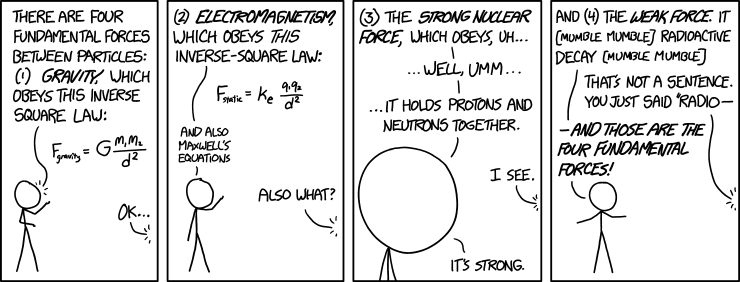
\includegraphics[scale=0.5]{fundamental_forces}

\begin{quote}
  \begin{itemize}
  \item[--]  Of these four forces, there's one we don't really understand.
  \item[--] Is it the weak force or the strong?
  \item[--]It's gravity.
  \end{itemize}
\end{quote}
\url{http://xkcd.com/1489/}

\section{Contenido de partículas}

\begin{frame}[fragile,allowframebreaks]
La materia conocida esta constituida de un cojunto de \emph{fermiones de Dirac} elementales definidos en la Tabla~\ref{tab:ef}
\begin{table}
  \centering
  \begin{tabular}{l|l|c|r}
    Tipo &Nombre & Simbolo&Carga\\\hline{}
   leptones& electrón & $e$& $-1$\\
          & neutrino & $\nu$ & $0$\\\hline{}
   quarks &quark up  & $u_1,u_2,u_3$ & $2/3$\\
          &quark down  & $d_1,d_2,d_3$& $-1/3$\\
  \end{tabular}
  \caption{Fermiones elementales:  The symbol represent both the particle, e.g $e^-$, as the antiparticle, e.g, $e^+$. The lectric chage is given in units of the electron chage $e$  }
  \label{tab:ef}
\end{table}
donde podemos definir los tripletes de color de quarks como
\begin{align}
  u=&
  \begin{pmatrix}
    u_1 \\ u_2\\ u_3\\
  \end{pmatrix}
  &d=&
  \begin{pmatrix}
    d_1 \\ d_2 \\ d_3\\
  \end{pmatrix}
\end{align}

Este conjunto de partículas esta bien definido para interacciones que conservan paridad como la interacción electromagnética o la fuerte. Para introducir la interacciones débiles usaremos más bien espinores de Weyl

\end{frame}

\section{Interacciones débiles}
\begin{frame}[fragile,allowframebreaks]
Las interacciones débiles son las responsables, entre otros fenoménos,
del decaimiento de neutrones libres en un protón, un electron y un
anti-neutrino electrónico. En nuestro entendimiento actual, se asume
que dicho decaimiento esta medidado por un bosón vectorial masivo y
cargado llamado $W^-_{\mu}$ con su correspondiente antipartícula
$W^{+}_{\mu}$. El caracter másivo da cuenta del corto alcance de la
interacción comparado con el rango infinito de la
interacción electromagnética mediada por un fotón sin masa
$A_{\mu}$. En la primera parte del decaimiento, el neutrón decae al
proton y un $W^{-}_{\mu}$ virtual, el cual a su vez decae en un
anti-neutrino derecho y un electrón izquierdo como se muestra en la
figura~\ref{fig:wnl}.

\begin{figure}
  \centering
  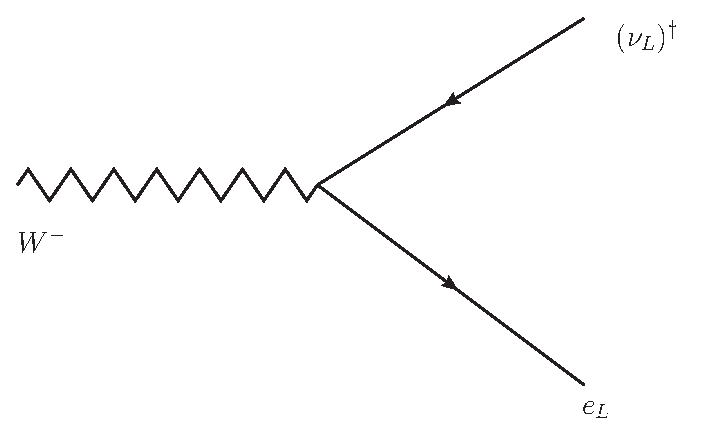
\includegraphics[scale=0.5]{wnl}
  \caption{Decaimiento del $W_\mu^-$.}
  \label{fig:wnl}
\end{figure}

Dicho decaimiento debe involucrar un término de interacción del tipo
\begin{align}
  \mathcal{L}_{W}\propto \left( \nu_L \right)^{\dagger}\overline{\sigma}^{\mu} e_L W_{\mu}^{+}.
\end{align}



Este tipo de interacción significa que en el contexto de las interacciones débiles un $e_L$ debe ser completamente
equivalente a un campo $\nu_L$. Es decir, el Lagrangiano debe ser
invariante bajo una transformación $\operatorname{SU}(2)_L$ de esos campos. A las energías normales, a las que se encuentra por ejemplo un neutrón dentro de un núcleo de Uranio, dicha simetría permanece oculta pues un electrón izquierdo y un neutrino izquierdo son campos completamente diferentes.
La
diferencia entre no sólo está en sus respectivas cargas eléctricas sino también
masas, pues la masa del neutrino es mucho más pequeña que la del electrón. 

Para poder explicar dicha interacción en el contexto de una simetría gauge local $\operatorname{SU}(2)_L$, debemos asumir que dicha simetría es explicita en alguna otra escala de energía donde en efecto  $e_L$ sea completamente
equivalente a $\nu_L$.

Debemos asumir entonces que ambos campos tienen una misma hipercarga,
asociada a una nueva simetría Abeliana $\operatorname{U}(1)_Y$ que sea la precursora de la simetría Abeliana de carga eléctrica $\operatorname{U}(1)_Q$. En tal caso, podríamos esperar que
la corriente electromagnética apropiada pueda obtenerse a partir del
Grupo semisimple $\operatorname{SU}(2)_L\times U(1)_Y$. Además. la respectiva masa para $W_{\mu}^{-}$
se podría obtener a partir del mecanismo de Higgs.

La simetría $\operatorname{SU}(2)_L$ entre las partes izquierdas del neutrino y el electrón, y entre las partes izquierdas de los quarks up y down, se establece  definiendo los dobletes:
  \begin{align}
    L\equiv\begin{pmatrix}
      \nu_L\\
      e_L      
    \end{pmatrix}\qquad   Q=&\begin{pmatrix}
    u_L\\
    d_L
  \end{pmatrix}\,,
  \end{align}
De otro lado, La invarianza bajo $U(1)_Y$ requiere que
\begin{align}
  Y_L=&Y_{\nu_L}=Y_{e_L}\nonumber\\
  Y_Q=&Y_{u_L}=Y_{d_L}\,.
\end{align}
El generador de carga eléctrica $\widehat{Q}$, se va obtener a partir de una combinación lineal del generador diagonal de $\operatorname{SU}(2)_L$, $T_3$, y del generador de hipercarga, $\widehat{Y}$.

Para considerar las interacciones débiles en conjunto con las interacciones electromágneticas y fuertes, es conveniente definir los campos de la primera generación en términos de los espinores ($\xi_{\alpha}$) y anti-espinores ($\eta^{\alpha}$) de Weyl izquierdos, de acuerdo a las convenciones de la Tabla~\ref{tab:electron}. El contenido de partículas con sus propiedades de transformación bajo el Grupo semisimple $\operatorname{SU}(3)_c\times \operatorname{SU}(2)_L\times U(1)_Y$ está dado en la Tabla~\ref{tab:fgw}, donde el $\mathbf{3}$ o el $\overline{\mathbf{3}}$ de $\operatorname{SU}(3)_c$ quieren decir que, además, para cada quark
\begin{align}
u_L=&
\begin{pmatrix}
  {u_{L}}_1\\
  {u_{L}}_2\\
  {u_{L}}_3
\end{pmatrix}&
  \left( u_R \right)^{\dagger}=&
  \begin{pmatrix}
    \left( u_R \right)^{\dagger}_1&
        \left( u_R \right)^{\dagger}_2&    \left( u_R \right)^{\dagger}_3
  \end{pmatrix},
\end{align}
etc.



\begin{table}
  \centering
  \begin{tabular}{l|c|c}\hline
    Nombre & Símbolo & $\left( \operatorname{SU}(3)_c, \operatorname{SU}(2)_L, U(1)_Y \right)$\\\hline
    $\Xi_{1\alpha}$: Doblete leptónico & $L=\displaystyle{\begin{pmatrix}
      \nu_L\\
      e_L      
    \end{pmatrix}}$ & $\left( \mathbf{1},\mathbf{2},Y_L \right)$\\
    $\Xi_{2\alpha}$: Doblete de quarks & $Q=\displaystyle{\begin{pmatrix}
      u_L\\
      d_L      
    \end{pmatrix}}$ & $\left( \mathbf{3},\mathbf{2},Y_Q \right)$\\
   $\eta^{\alpha}_1$: positrón izquierdo & $\left( e_R \right)^{\dagger}$&$\left(\mathbf{1},\mathbf{1},Y_{E}\right)$ \\
   $\eta^{\alpha}_2$: anti-up izquierdo & $\left( u_R \right)^{\dagger}$&$\left(\overline{\mathbf{3}},\mathbf{1},Y_{U}\right)$ \\
   $\eta^{\alpha}_3$: anti-down izquierdo & $\left( d_R \right)^{\dagger}$&$\left(\overline{\mathbf{3}},\mathbf{1},Y_{D}\right)$ \\
  \end{tabular}
  \caption{Spinores de Weyl izquierdos para la primera generación del modelo estándar}
  \label{tab:fgw}
\end{table}


Bajo la simetría $\operatorname{SU}(2)_L$, los campos transforman como:
 \begin{align}
  L\to L'=&\exp(i T^i \theta_i)L\approx(1+i T^i\theta_i)L\nonumber\\
  Q\to Q'=&\exp(i T^i \theta_i)Q\approx(1+i T^i\theta_i)Q\nonumber\\
  e_R\to& e'_R=e_R\nonumber\\
  u_R\to& u'_R=u_R\nonumber\\
  d_R\to& d'_R=d_R\,.
\end{align}
donde
\begin{align}
  T^i=\frac{\tau^i}{2}\,,
\end{align}
y $\tau^i$ son las matrices de Pauli dadas en la ec.~\eqref{eq:paulimatr}.

\end{frame}



\section{Simetría gauge local $\operatorname{SU}(3)_c\times  \operatorname{SU}(2)_L\times  U(1)_Y$}
\begin{frame}[fragile,allowframebreaks]
Los términos de masa de Dirac, usando las convenciones de la
Tabla~\ref{tab:fgw} no son invariantes bajo la simetría $\operatorname{SU}(2)_L$ porque
no hay forma de escribir términos escalares usando combinaciones los
campos $\Xi$ y $\eta$.  De la ec.~\eqref{eq:dwlag}, y usando la definición para los dobletes adjuntos de $\operatorname{SU}(2)_L$ en la ec.~\eqref{eq:Xiadj}, el Lagrangiano más
general posible para los campos de la Tabla~\ref{tab:fgw} compatibles
con las simetría de Lorentz y el grupo global $\operatorname{SU}(3)_c\times
\operatorname{SU}(2)_L\times U(1)_Y$ es
\begin{align}
  \mathcal{L}=&\sum_{i=1}^2i\epsilon_{ab}\widetilde{\Xi}_i^{a}\overline{\sigma}^{\mu}\partial_{\mu}\Xi_i^{b}
+\sum_{i=1}^3i\eta_{i}\sigma^{\mu}\partial_{\mu} \eta^{\dagger}_i\nonumber\\
  =&\sum_{i=1}^2i\widetilde{\Xi}_i\cdot\overline{\sigma}^{\mu}\partial_{\mu}\Xi_i
+\sum_{i=1}^3i\eta_{i}\sigma^{\mu}\partial_{\mu} \eta^{\dagger}_i\nonumber\\
=&i\widetilde{L}\cdot\overline{\sigma}^{\mu}\partial_{\mu}L+i\widetilde{Q}\cdot\overline{\sigma}^{\mu}\partial_{\mu}Q
+i(e_R)^{\dagger}\sigma^{\mu}\partial_{\mu} e_R+i(u_R)^{\dagger}\sigma^{\mu}\partial_{\mu} u_R+i
(d_R)^{\dagger}\sigma^{\mu}\partial_{\mu} d_R \nonumber\\
=&i(\nu_L)^{\dagger}\overline{\sigma}^{\mu}\partial_{\mu}\nu_L+i(e_L)^{\dagger}\overline{\sigma}^{\mu}\partial_{\mu}e_L
+i (u_L)^{\dagger}\overline{\sigma}^{\mu}\partial_{\mu}u_L+i(d_L)^{\dagger}\overline{\sigma}^{\mu}\partial_{\mu}d_L \nonumber\\
&+i(e_R)^{\dagger}\sigma^{\mu}\partial_{\mu}e_R+i(u_R)^{\dagger}\sigma^{\mu}\partial_{\mu} u_R+i(d_R)^{\dagger}\sigma^{\mu}\partial_{\mu} d_R \,,
\end{align}
donde
\begin{align}
\label{eq:widetildeLQ}
  \widetilde{L}=&
  \begin{pmatrix}
   \left(e_L\right)^{\dagger}\\
  - \left(\nu_L  \right)^{\dagger}\\
  \end{pmatrix},&
  \widetilde{Q}=&
  \begin{pmatrix}
   \left(d_L\right)^{\dagger}\\
  - \left(u_L  \right)^{\dagger}\\
  \end{pmatrix},&
\end{align}
de modo que
\begin{align*}
  i\widetilde{L}\cdot\overline{\sigma}^{\mu}\partial_{\mu}L=&
  i\,\epsilon_{ab}\widetilde{L}\cdot\overline{\sigma}^{\mu}\partial_{\mu}L \nonumber\\
 =&i\,\widetilde{L}^1\overline{\sigma}^{\mu}\partial_{\mu}L^2-i\,\left( -\widetilde{L}^2 \right)\overline{\sigma}^{\mu}\partial_{\mu}L^1    \nonumber\\
 =&i\,\left( e_L \right)^{\dagger}\overline{\sigma}^{\mu}\partial_{\mu}e_L+i\,\left( \nu_L \right)^{\dagger}\overline{\sigma}^{\mu}\partial_{\mu}\nu_L    \nonumber\\
\end{align*}
y lo mismo para $Q$.



Para obtener la interacciones del modelo estándar, reemplazamos las derivadas normales por derivadas covariantes.

Proponemos entonces el Lagrangiano
\begin{align}
\label{eq:L0}
     \mathcal{L}=&i\widetilde{Q}\cdot \overline{\sigma}^\mu\mathcal{D}_\mu Q+i\widetilde{L}\cdot \overline{\sigma}^\mu\mathcal{D}_\mu L+
i(e_R)^{\dagger}\sigma^\mu\mathcal{D}_\mu {e_R}+i(d_R)^{\dagger}\sigma^\mu\mathcal{D}_\mu d_R+i(u_R)^{\dagger}\sigma^\mu\mathcal{D}_\mu {u_R}
\nonumber\\
     &-\tfrac{1}{4}G^{\mu\nu}_a G_{\mu\nu}^a-\tfrac{1}{4}W^{\mu\nu}_i W_{\mu\nu}^i-\tfrac{1}{4}B^{\mu\nu} B_{\mu\nu}\,,
\end{align}
donde
\begin{align}
  \mathcal{D}^\mu&\equiv\partial^\mu-i g_s\frac{\lambda^a}{2}G^\mu_a-i g \frac{\tau^i}{2}W^\mu_i-i {g_1}YB^\mu\,.
\end{align}
y además
\begin{align*}
  \Lambda^a\equiv\frac{\lambda^a}{2},\ a=1,2,\ldots,8 &\qquad\text{8 generadores de $\operatorname{SU}(3)_c$}\\
  T^i\equiv\frac{\tau^i}{2},\ i=1,2,3 &\qquad\text{3 generadores de $\operatorname{SU}(2)_L$}\\
  Y &\qquad\text{generador de $U(1)_Y$},
\end{align*}
A este nivel, tanto los 15 fermiones de Weyl (cada quark izquierdo y derecho viene en tres colores), como los 12 bosones gauge, \emph{tienen masa nula}. Necesitamos entonces un mecanismo de ruptura espontánea de simetría para generar por lo menos masas para los tres bosones gauge asociados a la interacción débil, el cual será abordado en la Sección~\ref{sec:rupt-espont-de}.



\end{frame}
Además,
\begin{align}
  W_{\mu \nu}^i=&\partial_\mu W_\nu^i -\partial_\mu W_\mu^i+ g \epsilon_{ijk}W_\mu^j W_\nu^k \nonumber\\
  B_{\mu \nu}=&\partial_\mu B_\nu -\partial_\mu B_\mu\,.
\end{align}
y $G_{\mu\nu}^a$ está dado en la ec.~\eqref{eq:258qft}.

Bajo una transformación gauge local, las derivadas covariantes de los campos (y por consiguiente los campos) transforman como:
\begin{align}
  \mathcal{D}_\mu L&\to\left(\mathcal{D}_\mu L\right)'=\exp\left(-i\theta_iT^i-i\beta Y_L\right)\mathcal{D}_\mu L\nonumber\\
  \mathcal{D}_\mu Q&\to\left(\mathcal{D}_\mu Q\right)'=\exp\left(-i\alpha_a\Lambda^a-i\theta_iT^i-i\beta Y_Q\right)\mathcal{D}_\mu Q\nonumber\\
  \mathcal{D}_\mu \Phi&\to\left(\mathcal{D}_\mu \Phi\right)'=\exp\left(-i\theta_iT^i-i\beta Y_\Phi\right)\mathcal{D}_\mu \Phi\nonumber\\
  \mathcal{D}_\mu e_R&\to\left(\mathcal{D}_\mu e_R\right)'=\exp\left(-i\beta Y_{E}\right)\mathcal{D}_\mu e_R=\exp\left(-i\beta Q_{e}\right)\mathcal{D}_\mu e_R\nonumber\\
  \mathcal{D}_\mu d_R&\to\left(\mathcal{D}_\mu d_R\right)'=\exp\left(-i\alpha_a\Lambda^a-i\beta Y_{D}\right)\mathcal{D}_\mu d_R=\exp\left(-i\alpha_a\Lambda^a-i\beta Q_{d}\right)\mathcal{D}_\mu d_R\nonumber\\
  \mathcal{D}_\mu u_R&\to\left(\mathcal{D}_\mu u_R\right)'=\exp\left(-i\alpha_a\Lambda^a-i\beta Y_{U}\right)\mathcal{D}_\mu u_R=\exp\left(-i\alpha_a\Lambda^a-i\beta Q_{u}\right)\mathcal{D}_\mu u_R\,.
\end{align}
donde $Q_{e}=-1$, etc, son las cargas eléctricas asociadas a los campos.


\section{Ruptura espontánea de simetría}
\label{sec:rupt-espont-de}

\begin{frame}[fragile,allowframebreaks]
Todas las partículas en este lagrangiano son no masivas. Esto funciona sólo para los gluones y uno de los bosones gauge abelianos, pero no es realista para los bosones gauge cargados. 
Para solucionar este problema se postula la existencia de un nuevo doblete escalar complejo
( y su correspondiente adjunto de $\operatorname{SU}(2)$) con cuatro grados de libertad:
\begin{align}
\label{eq:Phi}
  \Phi=&
  \begin{pmatrix}
    \phi^+\\
    \phi^0\\
  \end{pmatrix}=
  \begin{pmatrix}
    \phi_1+i\phi_2\\
\phi_3+i\phi_4
  \end{pmatrix},&
\widetilde{\Phi}=&
  \begin{pmatrix}
    \left( \phi^0 \right)^{*}\\
   -\phi^-\\
  \end{pmatrix}\,.
\end{align}
El  ``$\pm$'' y el superíndice 0, se ponen de forma conveniente para obtener expresiones consitentes. Es claro que $\left( \phi^+ \right)^{*}=\phi^-\,.$





Es posible ahora construir invariantes $\operatorname{SU}(2)$ con las siguientes combinaciones de campos similares al del término de masa de Dirac en~\eqref{eq:dwlag}
\begin{align}
 -\eta_1\,\Xi_1\cdot\widetilde{\Phi}-\left(\eta_1\,\Xi_1\cdot\widetilde{\Phi}  \right)^{\dagger}
 =& -\eta_1\,\Xi_1\cdot\widetilde{\Phi}-\text{h.c}\nonumber\\
 =& -\eta^{b}_1\,\epsilon_{ab}\,\Xi_1^{a}\cdot\widetilde{\Phi}^{b}-\text{h.c} \nonumber\\
   =&-\left( e_R \right)^{\dagger}\epsilon_{ab}L^a\widetilde{\Phi}^b -\text{h.c} \nonumber\\
   =&\left( e_R \right)^{\dagger}L^1\widetilde{\Phi}^2+\left( e_R \right)^{\dagger}L^1\widetilde{\Phi}^2 +\text{h.c} \nonumber\\
   =&\left( e_R^{-} \right)^{\dagger}\nu_L\phi^- +\left( e_R^{-} \right)^{\dagger}e_L^-\phi^0 +\text{h.c} \,,
 \end{align}
donde $\text{h.c}$, denota el hermítico conjugado de cada término (para garantizar que el Lagrangiano sea real)
y hemos puesto la carga del electrón para hacer explícita la conservación de la carga eléctrica. 

Note que
\begin{align}
  \left( e_R \right)^{\dagger}\epsilon_{ab}L^a\widetilde{\Phi}^b=\left( e_R \right)^{\dagger}L\cdot \widetilde{\Phi}\,.
\end{align}


\end{frame}
\begin{frame}[fragile,allowframebreaks]
El Lagrangiano completo involucrando estos campos es
\begin{align}
     \mathcal{L}=&i\widetilde{Q}\cdot \overline{\sigma}^\mu\mathcal{D}_\mu Q+i\widetilde{L}\cdot \overline{\sigma}^\mu\mathcal{D}_\mu L+
i(e_R)^{\dagger}\sigma^\mu\mathcal{D}_\mu {e_R}+i(d_R)^{\dagger}\sigma^\mu\mathcal{D}_\mu {d_R}+i(u_R)^{\dagger}\sigma^\mu\mathcal{D}_\mu {u_R}
\nonumber\\
     &-\tfrac{1}{4}G^{\mu\nu}_a G_{\mu\nu}^a-\tfrac{1}{4}W^{\mu\nu}_i W_{\mu\nu}^i-\tfrac{1}{4}B^{\mu\nu} B_{\mu\nu}\nonumber\\
     &+\widetilde{\left( \mathcal{D}_\mu{\Phi} \right)}\cdot\mathcal{D}^\mu\Phi-\mu^2\widetilde{\Phi}\cdot\Phi-\lambda \left( \widetilde{\Phi}\cdot\Phi \right)^2\nonumber\\
     &- \left[  h_e \left( e_R \right)^{\dagger}\,L\cdot \widetilde{\Phi}_b +
      h_d \left( d_R \right)^{\dagger}\,Q\cdot \widetilde{\Phi} +
      h_u \left( u_R \right)^{\dagger}\,Q\cdot {\Phi}+\text{h.c}\right]\nonumber\\
     =&\mathcal{L}_{\text{fermion}}+\mathcal{L}_{\text{gauge}}
     +\mathcal{L}_{WBH}
     -\mathcal{L}_{\text{Yukawa}}\,.
\end{align}
donde $\mu^2<0$, y $\lambda>0$,
\begin{align}
  \widetilde{\Phi}=&i\tau_2\Phi^* 
% \nonumber\\
% =&i
% \begin{pmatrix}
%   0 & -i \\
%  i & 0\\
% \end{pmatrix}
% \begin{pmatrix}
%   \phi^+\\
% \phi^0
% \end{pmatrix}^{*} \nonumber\\
% =&\begin{pmatrix}
%   0 & 1 \\
%  -1 & 0\\
% \end{pmatrix}
% \begin{pmatrix}
%   \phi^-\\
% {\phi^0}^{*}
%\end{pmatrix} \nonumber\\
=\begin{pmatrix}
{\phi^0}^{*}\\
-  \phi^-\\
\end{pmatrix}, &   \Phi=&
  \begin{pmatrix}
    \phi^+\\
    \phi^0\\
  \end{pmatrix}.
\end{align}

\end{frame}
\begin{frame}[fragile,allowframebreaks]
Resumiendo

\begin{align}
  \label{eq:smscalar}
\mathcal{L}_{\text{fermion}}=&i\widetilde{Q}\cdot \overline{\sigma}^\mu\mathcal{D}_\mu Q+i\widetilde{L}\cdot \overline{\sigma}^\mu\mathcal{D}_\mu L \nonumber\\
&+i(e_R)^{\dagger}\sigma^\mu\mathcal{D}_\mu {e_R}+i(d_R)^{\dagger}\sigma^\mu\mathcal{D}_\mu {d_R}+i(u_R)^{\dagger}\sigma^\mu\mathcal{D}_\mu {u_R}\nonumber\\
  \mathcal{L}_{WBH}=&\widetilde{\left( \mathcal{D}_\mu{\Phi} \right)}\cdot\mathcal{D}^\mu\Phi-\mu^2\widetilde{\Phi}\cdot\Phi-\lambda \left( \widetilde{\Phi}\cdot\Phi \right)^2 \nonumber\\
\mathcal{L}_{\text{gauge}}=& -\tfrac{1}{4}G^{\mu\nu}_a G_{\mu\nu}^a-\tfrac{1}{4}W^{\mu\nu}_i W_{\mu\nu}^i-\tfrac{1}{4}B^{\mu\nu} B_{\mu\nu}\nonumber\\
  % =&(\mathcal{D}_\mu\Phi)^\dagger\mathcal{D}^\mu\Phi-\mu^2\Phi^\dagger\Phi-\lambda(\Phi^\dagger\Phi)^2\nonumber\\
%=&(\mathcal{D}_\mu\widetilde{\Phi})^\dagger\mathcal{D}^\mu\widetilde{\Phi}-\mu^2\widetilde{\Phi}^\dagger\widetilde{\Phi}-\lambda(\widetilde{\Phi}^\dagger\widetilde{\Phi})^2\nonumber\\
-\mathcal{L}_{\text{Yukawa}}=&  h_e \left( e_R \right)^{\dagger}\,L\cdot \widetilde{\Phi}_b +
      h_d \left( d_R \right)^{\dagger}\,Q\cdot \widetilde{\Phi} +
      h_u \left( u_R \right)^{\dagger}\,Q\cdot {\Phi}+\text{h.c}
\end{align}
Para el potencial escalar usaremos la forma más conveniente del producto matricial para el invariante de $\operatorname{SU}(2)_L$ por que no hay ambigüedad con el conjugado de un campo escalar.

Para los campos del Lagrangiano, debemos asegurarnos de que todos los términos invariantes gauge locales y renormalizables sean considerados. De hecho, términos de interacción entre fermiones y el campo escalar, correspondiente a una interacción de Yukawa, son invariantes bajo transformaciones $SU(3)_c\times  SU(2)_L\times  U(1)_Y$ si
\end{frame}
\begin{frame}[fragile,allowframebreaks]
\begin{align*}
  Y_L+Y_{\widetilde{\Phi}}-Q_{e}=&0\\
  Y_Q+Y_{\widetilde{\Phi}}-Q_{d}=&0\\
  Y_Q+Y_{\Phi}-Y_{u}=Y_Q-Y_{\widetilde{\Phi}}-Q_{u}=&0\,,
\end{align*}
donde hemos fijado $Y_{\widetilde{\Phi}}=-Y_\Phi$. Solucionado para las hipercargas de los dobletes tenemos
\begin{align}
\label{eq:yyy}
Y_L=&\frac{1}{2}\left( -Q_d+2Q_e+Q_u \right)=-\frac{1}{2}  \nonumber\\
Y_Q=&\frac{1}{2}\left( Q_d+Q_u \right)=\frac{1}{6} \nonumber\\
Y_{\widetilde{\Phi}}=-Y_{\Phi}=&\frac{1}{2}\left( Q_d-Q_u \right)=-\frac{1}{2}\,.
\end{align}

De este modo, es consistente interpretar los superíndices de $\phi^+$ y $\phi^0$ en la ec.~\eqref{eq:Phi} como las cargas eléctricas de las componentes del doblete de Higgs, $\Phi$.

\end{frame}

El potencial escalar contiene los términos
\begin{align}
  V(\Phi)=\mu^2\widetilde{\Phi}\cdot\Phi+\lambda \left( \widetilde{\Phi}\cdot\Phi \right)^2 
\end{align}
con $\mu^2<0$ y $\lambda>0$. % se reduce a
% \begin{align}
%   V(H)=\frac{1}{2}\mu^2(H+v)^2+\frac{1}{4}\lambda (H+v)^4\,.
% \end{align}


El modelo estándar es entonces una combinación de una teoría gauge local $\operatorname{SU}(3)_{c}$ con una simetría gauge local con ruptura espontánea de simetría (RES) $\operatorname{SU}(2)_L\times \operatorname{U}(1)_Y$. A continuación nos enfocaremos de momento en la parte leptónica de  $\operatorname{SU}(2)_L\times \operatorname{U}(1)_Y$ con RES.

\section{Una teoría para leptones de la primera generación}
\begin{frame}[fragile,allowframebreaks]
Comenzaremos analizando una versión simplificada del Lagrangiano con sólo los leptones de la primera de generación,
\begin{align}
  \mathcal{L}^{\text{lepton}}=\mathcal{L}_{\text{fermion}}^{\text{lepton}}+
   \mathcal{L}_{WBH}+\mathcal{L}_{\text{gauge}}-\mathcal{L}_{\text{Yukawa}}^{\text{lepton}}\,,
\end{align}
donde
\begin{align}
  \label{eq:smscalarlep}
\mathcal{L}_{\text{fermion}}^{\text{lepton}}=&i\widetilde{L}\cdot \overline{\sigma}^\mu\mathcal{D}_\mu L 
+i(e_R)^{\dagger}\sigma^\mu\mathcal{D}_\mu {e_R}\nonumber\\
  \mathcal{L}_{WBH}=&\widetilde{\left( \mathcal{D}_\mu{\Phi} \right)}\cdot\mathcal{D}^\mu\Phi-\mu^2\widetilde{\Phi}\cdot\Phi-\lambda \left( \widetilde{\Phi}\cdot\Phi \right)^2 \nonumber\\
\mathcal{L}_{\text{gauge}}=& -\tfrac{1}{4}W^{\mu\nu}_i W_{\mu\nu}^i-\tfrac{1}{4}B^{\mu\nu} B_{\mu\nu}\nonumber\\
  % =&(\mathcal{D}_\mu\Phi)^\dagger\mathcal{D}^\mu\Phi-\mu^2\Phi^\dagger\Phi-\lambda(\Phi^\dagger\Phi)^2\nonumber\\
%=&(\mathcal{D}_\mu\widetilde{\Phi})^\dagger\mathcal{D}^\mu\widetilde{\Phi}-\mu^2\widetilde{\Phi}^\dagger\widetilde{\Phi}-\lambda(\widetilde{\Phi}^\dagger\widetilde{\Phi})^2\nonumber\\
-\mathcal{L}_{\text{Yukawa}}^{\text{lepton}}=&  h_e \left( e_R \right)^{\dagger}\,L\cdot \widetilde{\Phi}_b +\text{h.c}
\end{align}
y sin perdida de generalidad para las partes del Lagrangiano $\mathcal{L}_{\text{gauge}}$ y $ \mathcal{L}_{WBH}\,$ que no involucran fermiones.
\end{frame}

\subsection{Interacciónes débiles fermión-gauge para leptones}

Nos enfocaremos de momento en la parte leptónica pues las interacciones para quarks involucran el mismo tipo de cálculos.

Los términos de interacción generados por la simetría gauge para el sector leptónico son:
\begin{align}
\label{eq:devLW}
 \mathcal{L}_{\text{fermion}}^{\text{lepton}}=& i \widetilde{L}\cdot\overline{\sigma}^\mu\mathcal{D}_\mu L+  i \left( e_R \right)^{\dagger}{\sigma}^\mu\mathcal{D}_\mu e_R \nonumber\\
=&i \widetilde{L}\cdot\overline{\sigma}^\mu\partial_\mu L+i \left(e_R  \right)^{\dagger}\sigma^\mu\partial_\mu {e_R} \nonumber\\
&+ i \widetilde{L}\cdot\overline{\sigma}^\mu(-i g_2 T_iW_\mu^i-i {g_1}\,Y_LB_\mu) L + i \left( e_R \right)^{\dagger}\sigma^\mu \left( -i{g_1} Y_R B_{\mu} \right) {e_R}\,.
\end{align}
Definiendo
\begin{align}
\label{eq:knt}
  \mathcal{L}_{\text{kinetic}}=&i \widetilde{L}\cdot\overline{\sigma}^\mu\partial_\mu L+i \left(e_R  \right)^{\dagger}\sigma^\mu\partial_\mu {e_R} \\
  \mathcal{L}_{WBL}=&i \widetilde{L}\cdot\overline{\sigma}^\mu(-i g_2 T_iW_\mu^i-i {g_1}\,Y_LB_\mu) L + i \left( e_R \right)^{\dagger}\sigma^\mu \left( -i{g_1} Y_R B_{\mu} \right) {e_R}\nonumber\,.
\end{align}
tenemos que
\begin{align}
\mathcal{L}_{WBL}=& \widetilde{L}\cdot\overline{\sigma}^\mu(g_2 T_1W_\mu^1+ g_2 T_2W_\mu^2+g_2 T_3W_\mu^3+{g_1}\,Y_LB_\mu) L+ g_1 Y_R\left(e_R \right)^{\dagger}\sigma^\mu  {e_R} B_\mu\nonumber\\
=& \widetilde{L}\cdot\overline{\sigma}^\mu\left[\frac{g_2}{\sqrt{2}}
  \begin{pmatrix}
0 & W_\mu^+\\
W_\mu^- & 0\\    
  \end{pmatrix}
+g_2 T_3W_\mu^3+{g_1}\,Y_LB_\mu
\right]L+ {g_1} Y_R\left(e_R \right)^{\dagger}\sigma^\mu  {e_R} B_\mu\nonumber\\
=&i \widetilde{L}\cdot\overline{\sigma}^\mu\frac{g_2}{\sqrt{2}}
  \begin{pmatrix}
0 & W_\mu^+\\
W_\mu^- & 0\\    
  \end{pmatrix}L+
 \widetilde{L}\cdot\overline{\sigma}^\mu\left[g_2 T_3W_\mu^3+{g_1}\,Y_LB_\mu
\right]L+ {g_1} Y_R\left(e_R \right)^{\dagger}\sigma^\mu  {e_R} B_\mu\nonumber\\
  =& \frac{g_2}{\sqrt{2}}\widetilde{L}\cdot\overline{\sigma}^\mu
  \begin{pmatrix}
e_LW_\mu^+\\
\nu_L W_\mu^-\\    
  \end{pmatrix}+\mathcal{L}_{A Z L}\,,
\end{align}

donde
\begin{align}
\label{eq:lazl}
  \mathcal{L}_{A Z L}=& \widetilde{L}\cdot\overline{\sigma}^\mu\left[g_2 T_3W_\mu^3+{g_1}\,Y_LB_\mu\right]L+ {g_1} Y_R\left(e_R \right)^{\dagger}\sigma^\mu  {e_R} B_\mu\,.
\end{align}

Teniendo en cuenta que 
\begin{align}
  \frac{g_2}{\sqrt{2}}\widetilde{L}\cdot\overline{\sigma}^\mu
  \begin{pmatrix}
e_LW_\mu^+\\
\nu_L W_\mu^-\\    
  \end{pmatrix}=\frac{g_2}{\sqrt{2}} \left[ \epsilon^{12} \widetilde{L}_1 \overline{\sigma}^{\mu} \nu_L W_{\mu}^-
+\epsilon^{21}  \widetilde{L}_2 \overline{\sigma}^{\mu} e_L W_{\mu}^+ \right],
\end{align}
y usando \eqref{eq:widetildeLQ}
\begin{align}
  \frac{g_2}{\sqrt{2}}\widetilde{L}\cdot\overline{\sigma}^\mu
  \begin{pmatrix}
e_LW_\mu^+\\
\nu_L W_\mu^-\\    
  \end{pmatrix}=\frac{g_2}{\sqrt{2}} \left[\left( e_L \right)^{\dagger} \overline{\sigma}^{\mu} \nu_L W_{\mu}^-
+ \left( \nu_L \right)^{\dagger} \overline{\sigma}^{\mu} e_L W_{\mu}^+ \right].
\end{align}
De este modo, la simetría gauge genera la interacción deseada con los bosones gauge cargados $W_{\mu}^{\pm}$. Sin embargo, se generan muchas otras interacciones las cuales deben contener apropiadamente la interacción electromagnética en algún cambio de base.

% Reemplazando en \eqref{eq:devLW}
% \begin{align}
%     i \widetilde{L}\cdot\overline{\sigma}^\mu\mathcal{D}_\mu L-i \widetilde{L}\cdot\overline{\sigma}^\mu\partial_\mu L
%   =&
% \frac{g_2}{\sqrt{2}}\left[\left( \nu_L \right)^{\dagger}\overline{\sigma}^\mu e_LW_\mu^++
% \left( e_L \right)^{\dagger}\overline{\sigma}^\mu\nu_L W_\mu^-\right]    
% +\mathcal{L}_{A Z L}\nonumber\\
%   =&
% \mathcal{L}_{W L}    
% +\mathcal{L}_{A Z L}\,,
% \end{align}
Entonces
\begin{align}
  \mathcal{L}_{WBL}= \mathcal{L}_{W L}+  \mathcal{L}_{A Z L}\,,
\end{align}
donde
\begin{align}
\label{eq:lwl}
  \mathcal{L}_{W L}=&\frac{g_2}{\sqrt{2}}\left[\left( \nu_L \right)^{\dagger}\overline{\sigma}^\mu e_LW_\mu^++
\left( e_L \right)^{\dagger}\overline{\sigma}^\mu\nu_L W_\mu^-\right].
\end{align}

El principal problema con $\mathcal{L}_{AZL}$ en la ec.~\eqref{eq:lazl} es que el neutrino izquierdo $\nu_L$ presente en $L$ se acopla a los dos bosones gauge neutros $W_3^{\mu}$ y $B^{\mu}$. Debemos buscar una base en la cual se pueda recuperar la interacción electromagnética de tal forma que el fotón $A_{\mu}$ no se acople a partículas neutras como el neutrino, $\nu_L$. Definimos entonces el posible fotón a partir de la rotación
\begin{equation}
\label{eq:rottw}
  \begin{pmatrix}
    W_3^\mu\\
    B^\mu
  \end{pmatrix}=\begin{pmatrix}
    \cos\theta_W & \sin\theta_W\\
    -\sin\theta_W& \cos\theta_W
  \end{pmatrix}
  \begin{pmatrix}
    Z^\mu\\
    A^\mu
  \end{pmatrix}.
\end{equation}
donde $\theta_{W}$, es el ángulo de rotación débil (Weak de sus siglas en inglés) y $Z^{\mu}$ es el otro campo que resulta de la rotación a la nueva base que define al fotón $A^{\mu}$.
Aplicando esta rotación a~\eqref{eq:lazl}, tenemos que
\begin{align}
\label{eq:brot}
   \mathcal{L}_{A Z L}=& \widetilde{L}\cdot\overline{\sigma}^\mu\left[g_2 T_3(c_W Z_\mu+s_W A_\mu)+{g_1}\,Y_L(-s_W Z_\mu+c_W A_\mu)\right]L
    +g_1 Y_R\left(e_R \right)^{\dagger}\sigma^\mu  {e_R} (-s_W Z_\mu+c_W A_\mu)\nonumber\\
     =& \widetilde{L}\cdot\overline{\sigma}^\mu\left[g_2 T_3c_W Z_\mu+g_2 T_3s_W A_\mu-{g_1}\,Y_Ls_W Z_\mu+{g_1}\,Y_Lc_W A_\mu\right]L\nonumber\\
&-g_1 s_W Y_R\left(e_R \right)^{\dagger}\sigma^\mu  {e_R}Z_{\mu}  +g_1 c_W Y_R\left(e_R \right)^{\dagger}\sigma^\mu  {e_R}A_{\mu}  \nonumber\\
    =& \widetilde{L}\cdot\overline{\sigma}^\mu\left[\left(g_2 c_WT_3-{g_1}s_W\,Y_L\right)Z_\mu
       +\left(g_2 s_W T_3+{g_1}c_W\,Y_L\right) A_\mu\right]L \nonumber\\
&-g_1 s_W Y_R\left(e_R \right)^{\dagger}\sigma^\mu  {e_R}Z_{\mu}  +g_1 c_W Y_R\left(e_R \right)^{\dagger}\sigma^\mu  {e_R}A_{\mu}  \,,
\end{align}
donde $c_W=\cos\theta_W$, $s_W=\sin\theta_W$. 

Para identificar $A_{\mu}$ con el fotón, debemos imponer la condición
\begin{align}
  \label{eq:relgn}
e\widehat{Q}=g_2 s_W T_3+{g_1}c_W\,\widehat{Y}\,.
\end{align}
De este modo
\begin{align}
  e\widehat{Q}L =& \left(g_2 s_W T_3+{g_1}c_W\,\widehat{Y}\right) L \nonumber\\
=& \left(g_2 s_W T_3+{g_1}c_W\,Y_L\right) L \,,
\end{align}
Usando la definición de $L$ tenemos que
\begin{align}
 e
  \begin{pmatrix}
    Q_{\nu} \nu_L\\
       Q_e e_L 
 \end{pmatrix}=
    e\begin{pmatrix}
   0\\
      Q_e e_L \\
  \end{pmatrix}=
  \begin{pmatrix}
   \left( \frac{1}{2}g_2 s_W +g_1 c_W Y_L \right) \nu_L\\ 
 \left(  -\frac{1}{2}g_2 s_W +g_1 c_W Y_L \right) e_L
  \end{pmatrix}
\end{align}
Igualando los coeficientes que acompañan los campos resultan las dos condiciones
\begin{align}
  \label{eq:g2sw}
  0= & \frac{1}{2}g_2 s_W +g_1 c_W Y_L  \\
    \label{eq:YL}
e Q_e=& \left(  -\frac{1}{2}g_2 s_W +g_1 c_W Y_L \right)
\end{align}
una tercera condición surge de imponer que el electrón derecho se acople apropiadamente al fotón
\begin{align}
  \label{eq:erel}
 e\widehat{Q} e_R =& \left(g_2 s_W T_3+{g_1}c_W\,\widehat{Y}\right) e_R\nonumber\\  
e Q_e e_R=& g_1 c_W\,Y_R \, e_R\,.
\end{align}
con estas condiciones podemos despejar tres incógnitas que corresponden a $g_1c_W$, $g_2s_W$ y $Y_L$.
La primera de ellas la podemos obtener de 
igualar los coeficientes que acompañan los campos para la tercera condición, teniendo en cuenta que $\widehat{Q}=\widehat{Y}$ para los campos derechos los cuales no participan de la interacción
débil asociada a $\operatorname{SU}(2)_L$
\begin{align}
  e=g_1 c_W\,.
\end{align}
Reemplazando en \eqref{eq:g2sw}
\begin{align}
  g_2 s_W = -2e Y_L\,,
\end{align}
y reemplazando ambos resultado en \eqref{eq:YL}, obtenemos
\begin{align}
  eQ_e=-\frac{1}{2} e+eY_L\,,
\end{align}
de donde podemos despejar $Y_L$ 
\begin{align}
  Y_L=Q_e+\frac{1}{2}=-1+\frac{1}{2}=-\frac{1}{2}\,.
\end{align}

El resultado final es entonces
\begin{align}
\label{eq:esc}
 Y_L=&-\frac{1}{2}\,,&   e=&g_2\sin\theta_W=g_1 \cos\theta_W\,.
\end{align}
La segunda ecuación se puede usara en la ec.~\eqref{eq:relgn} para obtener la predicción en término de los generadores diagonales válida para cualquier campo fermiónico
\begin{align}
\label{eq:gn}
 \widehat{Q}=&T_3+\widehat{Y}\,.
\end{align}

La ec. \eqref{eq:gn}, se conoce como la relación de Gell-Mann--Nishijima, y junto con~\eqref{eq:esc}, establece las condiciones que se deben satisfacer para obtener apropiadamente la QED a partir de la interacción electrodébil asociada al grupo semisimple $\operatorname{SU}(2)_L\times  U(1)_Y$.

\noindent
\textbf{Ejercicio}: Demostrar que los valores numéricos de las hipercargas en \eqref{eq:yyy} son consistentes con la relación de Gell-Mann--Nishijima \eqref{eq:gn}:
\begin{align}
 \widehat{Q}=&T_3+\widehat{Y}\,.
\end{align}


De la segunda ecuación  \eqref{eq:esc}, podemos expresar el ángulo $\theta_W$ en términos de $g_1$ y $g_2$ como
\begin{align}
\label{eq:twa}
  \tan\theta_W=\frac{g_1}{g_2}\,.
\end{align}

A modo de ilustración podemos comprobar
los valores numéricos para $Y_L$ y $Y_R$ usando directamente la relación de Gell-Mann--Nishijima \eqref{eq:gn}
\begin{align}
  \widehat{Q}L=&(T_3+Y_L)L \nonumber\\
  \begin{pmatrix}
    Q_\nu & 0\\
    0  & Q_e
  \end{pmatrix}
  \begin{pmatrix}
    \nu_L\\
    e_L
  \end{pmatrix}=  
  \begin{pmatrix}
   Q_{\nu} \nu_L\\
   Q_e e_L
  \end{pmatrix}
= & \begin{pmatrix}
    \frac{1}{2} + Y_L & 0\\
    0  & -\frac{1}{2}+Y_L
  \end{pmatrix}  \begin{pmatrix}
    \nu_L\\
    e_L
  \end{pmatrix} \,,
\end{align}
de modo que
\begin{align}
  Q_{\nu}&=0=\frac{1}{2}+Y_L\,, & Q_e&=-1=-\frac{1}{2}+Y_L\,,
\end{align}
lo cual  requiere que
\begin{align}
  Y_L=\frac{1}{2}\,.
\end{align}
De la misma forma
\begin{align}
  Y_R=Q_e=-1\,.
\end{align}
Note que para campos derechos la hipercarga coincide con la carga eléctrica.


Usando la relación entre $g_2$ y ${g_1}$~\eqref{eq:twa} en ~\eqref{eq:brot}
\begin{align}
    \mathcal{L}_{A Z L}
=&g_2 s_W \widetilde{L}\cdot\overline{\sigma}^\mu\left[\left(\cot\theta_WT_3- \tan\theta_W\,Y_L\right)Z_\mu
       +\left(T_3+Y_L\right) A_\mu\right]L \nonumber\\
&+g_2 s_W \left(e_R \right)^{\dagger}\sigma^\mu \left[ \left(0 -\tan\theta_W  Y_R  \right) Z_{\mu}  +\left( 0+ Y_R \right)  A_{\mu} \right]{e_R}\,,
\end{align}
donde hemos puesto explícitamente el cero correspondiente a: $T_3 e_R= 0 \,e_R$.

Como el generador asociado a $A_\mu$ debe ser el generador de carga eléctrica, podemos usar la primera ecuación en~\eqref{eq:esc}:
\begin{align}
  e=g_2\sin\theta_W\,,
\end{align}
y si además definimos
\begin{align}
  \mathcal{L}_{E}=g_2 s_W \left(e_R \right)^{\dagger}\sigma^\mu \left[ \left(0 -\tan\theta_W  Y_R  \right) Z_{\mu}  +\left( 0+ Y_R \right)  A_{\mu} \right]{e_R}\,,
\end{align}
tenemos que
\begin{align}
\label{eq:lazlf}
    \mathcal{L}_{A Z L}
=&e \widetilde{L}\cdot\overline{\sigma}^\mu\left(\cot\theta_W T_3-\tan\theta_W\,Y_L\right)L Z_\mu
       +e \widetilde{L}\cdot\gamma^\mu \widehat{Q} L A_\mu+\mathcal{L}_E\nonumber\\
=&e \widetilde{L}\cdot\overline{\sigma}^\mu\left[\cot\theta_W T_3-\tan\theta_W\left(\widehat{Q}-T_3\right)\right]L Z_\mu
       +e \widetilde{L}\cdot\overline{\sigma}^\mu \widehat{Q} L A_\mu + \mathcal{L}_E\nonumber\\
=&\phantom{+}\frac{e}{2c_W s_W} \widetilde{L}\cdot\overline{\sigma}^\mu\left[ \tau_3-2s_W^2\widehat{Q}\right]L Z_\mu
       +e \widetilde{L}\cdot\overline{\sigma}^\mu \widehat{Q} L A_\mu \nonumber\\
&+\frac{e}{2c_W s_W} \left( e_R \right)^{\dagger}{\sigma}^\mu\left[ 0-2s_W^2\widehat{Q}\right]e_R\, Z_\mu
       +e \left( e_R \right)^{\dagger}{\sigma}^\mu \widehat{Q} e_R\, A_\mu \nonumber\\
=&\mathcal{L}_{ZL}+\mathcal{L}^{\text{int}}_{\text{QED}} \,,
\end{align}
donde
\begin{align}
  \label{eq:LQED}
     \mathcal{L}^{\text{int}}_{\text{QED}}=&e \widetilde{L}\cdot\overline{\sigma}^\mu \widehat{Q} L A_\mu+
e \left( e_R \right)^{\dagger}{\sigma}^\mu \widehat{Q} e_R\, A_\mu \\
\mathcal{L}_{ZL}=&\frac{e}{2c_W s_W} \widetilde{L}\cdot\overline{\sigma}^\mu\left[ \tau_3-2s_W^2\widehat{Q}\right]L Z_\mu
+\frac{e}{2c_W s_W} \left( e_R \right)^{\dagger}{\sigma}^\mu\left[ 0-2s_W^2\widehat{Q}\right]e_R\, Z_\mu\,.
\end{align}
Como las expresiones están en términos de los generadores como operadores, deberían ser válidas para otros conjuntos apropiados de fermiones para ser definidos más adelante.


De  la ecuación \eqref{eq:LQED}
\begin{align}
     \mathcal{L}^{\text{int}}_{\text{QED}}=&e \widetilde{L}\cdot\overline{\sigma}^\mu \widehat{Q} L A_\mu+
e \left( e_R \right)^{\dagger}{\sigma}^\mu \widehat{Q} e_R\, A_\mu \nonumber\\
=&-e \left[ \left( e_L \right)^{\dagger}\overline{\sigma}^\mu \ e_L + \left( e_R \right)^{\dagger}{\sigma}^\mu \ e_R  \right]A_{\mu}\,,
\end{align}
y la interacción de la electrodinámica cuántica se recupera satisfactoriamente.

\begin{frame}[fragile,allowframebreaks]
Para obtener la interacción requerida de los $W^{\pm}$ con el $\nu_L$ y $e_L$ dada en la ec~\eqref{eq:lwl} y genera el fotón con las propiedades adecuadas resumidas en la ec.~\eqref{eq:LQED}, el modelo gauge local $\operatorname{SU}(2)_L\times \operatorname{U}(1)_Y$ predice entonces la existencia de nuevas interacciones con un nuevo bosón gauge $Z_{\mu}$ dadas por
\begin{align}
  \label{eq:zneus}
\mathcal{L}_{ZL}
=&\frac{e}{2c_W s_W} \widetilde{L}\cdot\overline{\sigma}^\mu\left[ \tau_3-2s_W^2\widehat{Q}\right]L Z_\mu
+\frac{e}{2c_W s_W} \left( e_R \right)^{\dagger}{\sigma}^\mu\left[ 0-2s_W^2\widehat{Q}\right]e_R\, Z_\mu \nonumber\\
  =&\frac{e}{2c_W s_W} \left\{ \left( \nu_L \right)^{*}\overline{\sigma}^\mu \nu_L
    + \left( e_L \right)^{*}\overline{\sigma}^\mu\left[ -1+2s_W^2\right]e_L
     +2s_W^2 \left( e_R \right)^{\dagger}{\sigma}^\mu e_R 
     \right\}Z_\mu \nonumber\\
 =&\frac{e}{2c_W s_W} \left\{ \left( \nu_L \right)^{*}\overline{\sigma}^\mu \nu_L
    - \left( e_L \right)^{*}\overline{\sigma}^\mu e_L 
    +2s_W^2 \left[\left( e_L \right)^{*}\overline{\sigma}^\mu e_L+
    \left( e_R \right)^{\dagger}{\sigma}^\mu e_R    \right]  
     \right\}Z_\mu\,.     
\end{align}
\end{frame}
Vemos entonces que el $Z_{\mu}$ tiene acoplamientos a las partes izquierdas
de los leptones y otro acoplamiento que no diferencia partes izquierdas y derechas similar al del fotón, pero
suprimido por $2\sin^2\theta_W$.


Una predicción bastante concreta es que los neutrinos izquierdos se acoplan con el nuevo bosón gage neutro a través del término de interacción
\begin{align}
\mathcal{L}_{Z\nu}=  \frac{e}{2c_W s_W}\left( \nu_L \right)^{\dagger} \overline{\sigma}^{\mu} \nu_L Z_\mu\,,
\end{align}
que implica la existencia de corrientes neutras en carga eléctrica y por lo tanto abren la posibilidad de un desbalance de energía completo en colisiones electrón positrón. Dichas corrientes fueron medidas en 1971 y permitieron una primera determinación de los valores experimentales para $g_2$ y $\theta_W$.


Resumiendo
\begin{align}
  \label{eq:fermlep}
  \mathcal{L}_{\text{fermion}}^{\text{lepton}}=& i \widetilde{L}\cdot\overline{\sigma}^\mu\mathcal{D}_\mu L+  i \left( e_R \right)^{\dagger}{\sigma}^\mu\mathcal{D}_\mu e_R \nonumber\\
 =&\mathcal{L}_{\text{kinetic}}+
\mathcal{L}_{WL}+\mathcal{L}^{\text{int}}_{\text{QED}}+ \mathcal{L}_{ZL}\,,
\end{align}
dados en las ecs.~\eqref{eq:knt}, \eqref{eq:lwl}, \eqref{eq:LQED} y \eqref{eq:zneus}.


Note que a este nivel el bosón gauge $Z_{\mu}$ es no masivo. Sin embargo para explicar porque dicha interacción no había sido observada al momento de su predicción se tiene que asumir que el bosón gauge $Z_{\mu}$ debe ser muy masivo para que la interacción sea de corto alcance y por consiguiente suprimida con respecto a la de bosones gauge sin masa. 

Por lo tanto, para obtener una teoría realista se debe adicionar un mecanismo de ruptura espontánea de simetría para dar masa a los tres bosones $W_{\mu}^{+}$, $W_{\mu}^{-}$ y $Z_{\mu}$. Dicho mecanismo será discutido en la Sección~\ref{sec:el-gauge-unitario}.



\subsection{El gauge unitario}
\label{sec:el-gauge-unitario}

\begin{frame}[fragile,allowframebreaks]
Retornando al doblete de Higgs del modelo estándar en la ec.~\eqref{eq:polarhiggs}, los cuatro grados de libertad de $\Phi$, pueden escribirse en forma polar con la parte real neutra desplazada para generar la ruptura espontánea de la simetría $\operatorname{SU}(2)_L\times  U(1)_Y$. De este modo, y sin perdida de generalidad
\begin{align}
\label{eq:92qft}
  {\Phi}=&e^{i G_j(x)T^j}
  \begin{pmatrix}
    0\\
    \frac{1}{\sqrt{2}}[H(x)+v]
  \end{pmatrix}.
\end{align}

Para $\operatorname{SU}(2)_L\times  U(1)_Y$ tenemos cuatro generadores y cuatro bosones gauge. De acuerdo a la parametrización en ec.~\eqref{eq:92qft} esperamos que aparezcan tres bosones de Goldstone y un campo de Higgs con masa, de manera que quedará un generador no roto correspondiente a una simetría remanente del vacío $U(1)_Q$
\begin{equation}
  \operatorname{SU}(2)_L\times  U(1)_Y\overset{\langle\widetilde{\Phi}\rangle}{\longrightarrow}U(1)_Q.
\end{equation}

Se espera entonces que el espectro consista de un bosón de Higgs, tres bosones gauge masivos, y un bosón gauge sin masa.

Podemos hacer una transformación gauge similar a la de la 
%DEBUG: corregir
ec.~\eqref{eq:93qft} sobre el campo $\widetilde{\Phi}$, tal que
\begin{equation}
  \label{eq:123qft}
    {\Phi}\to{\Phi}'=
  \begin{pmatrix}
    0\\
    \frac{1}{\sqrt{2}}(H(x)+v)
  \end{pmatrix},
\end{equation}
que define el \emph{gauge unitario}. En adelante sin embargo omitiremos las primas sobre los campos transformados ${\Phi}'$ y $W'_{\mu\nu}$.

Comenzaremos analizando la parte escalar del Lagrangiano del Modelo dada en la ec.~\eqref{eq:smscalar} en el gauge unitario
\begin{align}
  \mathcal{L}_{WBH}
  =&\widetilde{\left( \mathcal{D}_\mu{\Phi} \right)}\cdot\mathcal{D}^\mu\Phi-\mu^2\widetilde{\Phi}\cdot\Phi-\lambda \left( \widetilde{\Phi}\cdot\Phi \right)^2 \nonumber\\
  =&\frac{1}{2}\widetilde{\left[\mathcal{D}^\mu \begin{pmatrix}
    0\\
    H(x)+v
  \end{pmatrix}\right]}\cdot \mathcal{D}_\mu\begin{pmatrix}
    0\\
    H(x)+v
  \end{pmatrix}-V(H)\,,
\end{align}
donde $V(H)$ dado en la ec.~\eqref{eq:higgspot}, incluye el término de masa para el bosón de Higgs \eqref{eq:higgsmass}:
\begin{equation}
  m_H^2=2\left|\mu^2\right|=2\lambda v^2
\end{equation}
De la ec.~\eqref{eq:w22}
\begin{align}
      W_\mu=&\begin{pmatrix}
    \frac{1}{2}W_3&\frac{1}{\sqrt{2}}W^+_\mu\\
    \frac{1}{\sqrt{2}}W^-_\mu&-\frac{1}{2}W^3_\mu
  \end{pmatrix}.
\end{align}
$\mathcal{D}_\mu$ corresponde a la matrix $2\times  2$, dada en la ec.~\eqref{eq:d22}, con el reemplazo
\begin{align}
\mp\frac{i}{2}g_2 W^3_\mu\to  -i\left(\pm\frac{1}{2}g_2 W^3_\mu+{g_1}Y B_\mu\right)
\end{align}

\begin{align}
  \label{eq:dercovsu2L}
 \mathcal{D}_\mu &=  \begin{pmatrix}
    \partial_\mu-i\left(\frac{1}{2}g_2 W^3_\mu+{\color{red}{g_1} Y B_\mu}\right)&-\frac{i}{\sqrt{2}}g_2 W^+_\mu\\
    -\frac{i}{\sqrt{2}}g_2 W^-_\mu&\partial_\mu-i\left(-\frac{1}{2}g_2 W^3_\mu+{\color{red}{g_1}Y B_\mu}\right)
  \end{pmatrix}.
\end{align}

Entonces
\begin{align}
\mathcal{D}_\mu \begin{pmatrix}
    0\\
    H(x)+v
  \end{pmatrix}=\begin{pmatrix}
    -\frac{i}{\sqrt{2}}gW_\mu^+(H+v)\\
    \partial_\mu H-i\left(-\frac{1}{2}gW^3_\mu+{\color{red}{g_1}Y_{\widetilde{\Phi}} B_\mu}\right)(H+v)
  \end{pmatrix}.
\end{align}

El correspondiente productor escalar $\operatorname{\operatorname{SU}}(2)_L$ es:
\begin{align}
  \mathcal{L}_{WBH}=&\frac{1}{2}\widetilde{\begin{pmatrix}
    -\frac{i}{\sqrt{2}}g{W^\mu}^+(H+v)\\
    \partial^\mu H-i\left(-\frac{1}{2}gW_3^\mu+{g_1}Y_{\widetilde{\Phi}} B^\mu\right)(H+v)
  \end{pmatrix}}\cdot
   \begin{pmatrix}
    -\frac{i}{\sqrt{2}}gW_\mu^+(H+v)\\
    \partial_\mu H-i\left(-\frac{1}{2}gW^3_\mu+{g_1}Y_{\widetilde{\Phi}} B_\mu\right)(H+v)
  \end{pmatrix}-V(H)\nonumber\\
=&\frac{1}{2}\begin{pmatrix}
    \partial^\mu H+i\left(-\frac{1}{2}gW_3^\mu+{g_1}Y_{\widetilde{\Phi}} B^\mu\right)(H+v)\\
    \frac{i}{\sqrt{2}}g{W^\mu}^-(H+v)\\
  \end{pmatrix}\cdot
  \begin{pmatrix}
    -\frac{i}{\sqrt{2}}gW_\mu^+(H+v)\\
    \partial_\mu H-i\left(-\frac{1}{2}gW^3_\mu+{g_1}Y_{\widetilde{\Phi}} B_\mu\right)(H+v)
  \end{pmatrix}-V(H)\nonumber\\
  =&\frac{1}{4}g^2{W^\mu}^-W_\mu^+(H+v)^2-V(H)\nonumber\\
  &+\frac{1}{2}\left[\partial^\mu H+i\left(-\tfrac{1}{2}gW_3^\mu+{g_1}Y_{\widetilde{\Phi}} B^\mu\right)(H+v)\right]
  \times\nonumber\\
  &\qquad\left[\partial_\mu H-i\left(-\tfrac{1}{2}gW^3_\mu+{g_1}Y_{\widetilde{\Phi}} B_\mu\right)(H+v)\right]\nonumber\\
 =&-V(H)
  +\frac{1}{4}g^2{W^\mu}^-W_\mu^+(H+v)^2+\nonumber\\
  &+\frac{1}{2}\partial^\mu H\partial_\mu H+\frac{1}{2}\left(-\tfrac{1}{2}gW_3^\mu+{\color{red}{g_1}Y_{\widetilde{\Phi}} B^\mu}\right)^2(H+v)^2
\end{align}
donde la última línea corresponde a la magnitud del ``número'' complejo: 
\begin{align}
\left[\partial_\mu H-i\left(-\tfrac{1}{2}gW^3_\mu+{g_1}Y_{\widetilde{\Phi}} B_\mu\right)(H+v)\right]
\end{align}

\end{frame}
\begin{frame}[fragile,allowframebreaks]

Entonces
\begin{align}
  \label{eq:96qft}
  \mathcal{L}_{WBH}=&\frac{1}{2}\partial^\mu H\partial_\mu H-V(H)
  +\frac{g^2v^2}{4}{W^\mu}^-W_\mu^+ \left( \frac{H}{v}+1 \right)^2+\mathcal{L}_{Z A H}\,,
\end{align}
donde
\begin{align}
  \mathcal{L}_{ZAH}=\frac{1}{2}&\left(\tfrac{1}{4}g^2W_3^\mu W^3_\mu-\tfrac{1}{2}g{g_1}Y_{\widetilde{\Phi}} W_3^\mu B_\mu-\tfrac{1}{2}g{g_1}Y_{\widetilde{\Phi}} W_3^\mu B_\mu+{{g_1}}^2Y_{\widetilde{\Phi}} ^2B^\mu B_\mu\right)
\left(H+v\right)^2.
\end{align}
Haciendo $Y_{\widetilde{\Phi}} =1/2$ como en la ec.~\eqref{eq:yyy},
\begin{align}
  \mathcal{L}_{ZAH}=\frac{1}{2}\frac{v^2}{4}
  \begin{pmatrix}
    W^\mu_3 & B^\mu
  \end{pmatrix}
  \begin{pmatrix}
    g^2_2&-g_2{g_1}\\
    -g_2{g_1}&g_1^2
  \end{pmatrix}
  \begin{pmatrix}
    W^3_\mu\\
    B_\mu
  \end{pmatrix}
\left(\frac{H}{v}+1\right)^2\,.
\end{align}
Sea
\begin{equation}
  V=\begin{pmatrix}
    \cos\theta_W & \sin\theta_W\\
    -\sin\theta_W& \cos\theta_W
  \end{pmatrix}=
  \frac{1}{\sqrt{g^2_2+g_1^2}}\begin{pmatrix}
    g_2   & {g_1}\\
    -{g_1} & g_2
  \end{pmatrix},
\end{equation}
con $\tan\theta_W={g_1}/g$, tal que $g\sin\theta_W={g_1}\cos\theta_W$, como en la ec.~\eqref{eq:esc}. De esta forma podremos comprobar si la misma condición que hace que los neutrinos no se acoplen con el fotón, garantiza el campo neutro $H$ tampoco se acopla directamente con el fotón. 

Note que $V$ es una matrix ortogonal que satisface $VV^T=V^TV=\mathbf{1}$. Si (ver ec.~\eqref{eq:rottw}),
\begin{align}
  \begin{pmatrix}
    W^3_\mu\\
    B_\mu
  \end{pmatrix}=&V
  \begin{pmatrix}
    Z_\mu\\
    A_\mu
  \end{pmatrix}&\text{ó}\qquad
  \begin{pmatrix}
    Z_\mu\\
    A_\mu
  \end{pmatrix}=&V^T
  \begin{pmatrix}
    W^3_\mu\\
    B_\mu
  \end{pmatrix}
\end{align}
entonces
\begin{align}
  \mathcal{L}_{ZAH}=&\frac{1}{2}\frac{v^2}{4}
  \begin{pmatrix}
    W^{3\mu} & B^\mu
  \end{pmatrix}VV^T
  \begin{pmatrix}
    g^2&-g_2{g_1}\\
    -g_2{g_1}&g_1^2
  \end{pmatrix}VV^T
  \begin{pmatrix}
    W^3_\mu\\
    B_\mu
  \end{pmatrix}
\left(\frac{H}{v}+1\right)^2\nonumber\\
=&\frac{1}{2}\frac{v^2}{4}
  \begin{pmatrix}
    Z^\mu & A^\mu
  \end{pmatrix}\left[V^T
  \begin{pmatrix}
    g_2^2&-g_2{g_1}\\
    -g_2{g_1}&g_1^2
  \end{pmatrix}V\right]
  \begin{pmatrix}
    Z_\mu\\
    A_\mu
  \end{pmatrix}
\left(\frac{H}{v}+1\right)^2
\end{align}
\begin{align}
  V^T
  \begin{pmatrix}
    g_2^2&-g_2{g_1}\\
    -g_2{g_1}&{{g_1}}^2
  \end{pmatrix}V=&\frac{1}{g_2^2+{{g_1}}^2}
  \begin{pmatrix}
    g_2^3+g{{g_1}}^2 & -g_2^2{g_1}-{{g_1}}^3\\
+g_2^2{g_1}-g_2^2{g_1}    &-g_2 g_1^2+g_2 g_1^2
  \end{pmatrix}
\begin{pmatrix}
    g_2   & {g_1}\\
    -{g_1} & g_2
  \end{pmatrix}\nonumber\\
=&\frac{1}{g_2^2+{{g_1}}^2}
  \begin{pmatrix}
    g_2^3+g_2 g_1^2 & -g_2^2{g_1}-g_1^3\\
    0   &0
  \end{pmatrix}
\begin{pmatrix}
    g_2   & {g_1}\\
    -{g_1} & g_2
  \end{pmatrix}\nonumber\\
=&\frac{1}{g_2^2+{{g_1}}^2}
  \begin{pmatrix}
    g_2^4+g^2 g_1^2+g_2^2 g_1^2+g_1^4 & g_2^3{g_1}+g_2 g_1^3-g_2^3{g_1}-g_2 g_1^3\\
    0    &0
  \end{pmatrix}\nonumber\\
=&\begin{pmatrix}
    g_2^2+g_1^2 & 0\\
    0    &0
  \end{pmatrix}
\end{align}
De este modo

\begin{align}
  \mathcal{L}_{ZAH}&=\frac{1}{2}\frac{v^2}{4}\left(g_2^2+g_1^2\right)Z^\mu Z_\mu
  \left(\frac{H}{v}+1\right)^2\nonumber\\
 &=\frac{1}{2}\left(\frac{g_2v}{2}\right)^2\left(1+\tan^2\theta_W\right)Z^\mu Z_\mu
             \left(\frac{H}{v}+1\right)^2\nonumber\\
   &=\frac{1}{2}\left(\frac{g_2v}{2\cos\theta_W}\right)^2Z^\mu Z_\mu\left(\frac{H}{v}+1\right)^2\,.
\end{align}
Retornando a la ec.~(\ref{eq:96qft}), tenemos
tenemos
\begin{align}
  \label{eq:lwbhfin}
  \mathcal{L}_{W B H}=&\widetilde{\left( \mathcal{D}_\mu{\Phi} \right)}\cdot\mathcal{D}^\mu\Phi-\mu^2\widetilde{\Phi}\cdot\Phi-\lambda \left( \widetilde{\Phi}\cdot\Phi \right)^2 \nonumber\\
  =&\frac{1}{2}\partial^\mu H\partial_\mu H-V(H)\nonumber\\
  &+\frac{1}{2}m_W^2{W^\mu}^-W_\mu^+ \left(\frac{H}{v}+1 \right)^2
    +\frac{1}{2}m_W^2{W^\mu}^-W_\mu^+\left(\frac{H}{v}+1 \right)^2
    +\frac{1}{2}m_Z^2Z^\mu Z_\mu\left(\frac{H}{v}+1 \right)^2,
\end{align}
donde el termino $1$ en la expansión binomial $\left({H}/{v}+1 \right)^2$ corresponde al
término de masa en cada caso:
%instiki:
\begin{itemize} %noinstiki
\item Masas gauge:
\begin{equation}
\label{eq:mwz}
  m_W=\frac{g_2v}{2}
  \qquad 
  m_Z=\frac{g_2v}{2\cos\theta_W},
\end{equation}
y
\begin{equation}
\label{eq:mwzw}
  m_Z=\frac{m_W}{\cos\theta_W}.
\end{equation}
\item Ver eq.~\eqref{eq:higgspot}
  \begin{align}
    V(H)=&\tfrac{1}{2}m_H^2H^2+\lambda vH^3+\tfrac{1}{4}\lambda H^4\nonumber\\
    =&\frac{1}{2}m_H^2 H^2\left( \frac{H}{2v}+ 1 \right)^2\,,
  \end{align}
con
\begin{equation}
  m_H^2=-2\mu^2=2\lambda v^2,
\end{equation}
además:
\item 
\begin{equation}
\label{eq:azmix}
  \begin{pmatrix}
    W^3_\mu\\
    B_\mu
  \end{pmatrix}=\begin{pmatrix}
    \cos\theta_W & \sin\theta_W\\
    -\sin\theta_W& \cos\theta_W
  \end{pmatrix}
  \begin{pmatrix}
    Z_\mu\\
    A_\mu
  \end{pmatrix},
\end{equation}
tal que
\begin{equation}
  \label{eq:tw}
  g_2\sin\theta_W={g_1}\cos\theta_W\,.
\end{equation}
\end{itemize} %noinstiki
%instiki:

\end{frame}

\bigskip
\noindent
\textbf{Ejercicio}: Demostrar que

\begin{align}
  \mathcal{L}_{\text{fermion}}^{\text{lepton}}=& i \widetilde{L}\cdot\overline{\sigma}^\mu\mathcal{D}_\mu L+  i \left( e_R \right)^{\dagger}{\sigma}^\mu\mathcal{D}_\mu e_R \nonumber\\
 =&\mathcal{L}_{\text{kinetic}}+
\mathcal{L}_{WL}+\mathcal{L}^{\text{int}}_{\text{QED}}+ \mathcal{L}_{ZL}\,,
\end{align}
dados en las ecs.~\eqref{eq:knt}, \eqref{eq:lwl}, \eqref{eq:LQED} y \eqref{eq:zneus}, usando directamente la expresión para la derivada covariante para un doblete, en esta caso $L$, dada  en la ec.~\eqref{eq:dercovsu2L}.


\subsection{Auto interacciones}

\begin{frame}[fragile,allowframebreaks]
El Lagrangiano gauge
\begin{align}
  \mathcal{L}_{\text{gauge}}=& -\tfrac{1}{4}G^{\mu\nu}_a G_{\mu\nu}^a-\tfrac{1}{4}W^{\mu\nu}_i W_{\mu\nu}^i-\tfrac{1}{4}B^{\mu\nu} B_{\mu\nu}\,,
\end{align}
Se debe expresar en la base de $Z_\mu$, $A_\mu$. Los detalles están en \url{https://www.overleaf.com/read/pxkqqdhrqyrk}
\begin{align}
\label{eq:lgaguefin}
\mathcal{L}_{\text{gauge}}=&  -\tfrac{1}{4}F^{\mu\nu} F_{\mu\nu}-\tfrac{1}{4}Z^{\mu\nu} Z_{\mu\nu}-\tfrac{1}{2}(F_W^\dagger)^{\mu\nu} (F_W)_{\mu\nu}
- \tfrac{1}{4}\widetilde{G}^{\mu\nu}_a \widetilde{G}_{\mu\nu}^a\nonumber\\
&-ie\cot\theta_W\left[(F_W^\dagger)^{\mu\nu}W_\mu^+ Z_\nu-(F_W)^{\mu\nu}W_\mu^- Z_\nu+W_\mu^-W_\nu^+Z^{\mu\nu}\right]\nonumber\\
&-ie\left[(F_W^\dagger)^{\mu\nu}W_\mu^+ A_\nu-(F_W)^{\mu\nu}W_\mu^- A_\nu+W_\mu^-W_\nu^+F^{\mu\nu}\right]\nonumber\\
&-\frac{e^2}{2\sin^2\theta_W}\left[\left(W_\mu^+{W^\mu}^-\right)^2-W_\mu^+{W^\mu}^+W_\nu^-{W^\nu}^-\right] \nonumber\\
&-e^2\cot^2\theta_W\left(W_\mu^+{W^\mu}^-Z_\nu Z^\nu-W_\mu^+Z^\mu W_\nu^-Z^\nu\right)\nonumber\\
&-e^2\cot^2\theta_W\left(2W_\mu^+{W^\mu}^-A_\nu Z^\nu-W_\mu^+A^\mu W_\nu^-Z^\nu-W_\mu^+Z^\mu W_\nu^-A^\nu\right)\nonumber\\
&-e^2\left(W_\mu^+{W^\mu}^-A_\nu A^\nu-W_\mu^+A^\mu W_\nu^-A^\nu\right),
\end{align}
donde
\begin{align}
  {F}^{\mu\nu}=&\partial^\mu A^\nu_a-\partial^\nu A^\mu\,, &  (F_W)_{\mu\nu}=&\partial_\mu W^+_\nu-\partial_\nu W^+_\mu\nonumber\\
  {Z}^{\mu\nu}=&\partial^\mu Z^\nu_a-\partial^\nu Z^\mu\,,& &% \widetilde{G}^{\mu\nu}=&\partial^\mu G^\nu_a-\partial^\nu G^\mu\,.
\end{align}

\end{frame}


\subsection{Lagrangiano  de Yukawa para leptones}

\begin{frame}[fragile,allowframebreaks]
En el gauge unitario
\begin{align}
  \label{eq:lyuklep}
  \mathcal{L}_{\text{Yukawa}}^{\text{lepton}}=& h_e \left( e_R \right)^{\dagger}\,\epsilon^{ab}L_a\widetilde{\Phi}_b+\text{h.c}\nonumber\\
=&\frac{h_e}{\sqrt{2}}\left[\left( e_L \right)^{\dagger}e_R+\left( e_R \right)^{\dagger}e_L\right]
\left[H(x)+v\right]\nonumber\\
=&\frac{h_ev}{\sqrt{2}}\left[\left( e_L \right)^{\dagger}e_R+\left( e_R \right)^{\dagger}e_L\right]
\left[\frac{H(x)}{v}+1\right].
\end{align}
Note que de forma autoconsistente
\begin{align}
 -Y_R+ Y_L-Y_{\Phi}= -Q_e+ Y_L-Y_{\Phi}=1-1/2-1/2=0\,.
\end{align}


Definiendo
\begin{align}
  m_e=\frac{h_ev}{\sqrt{2}}
\end{align}
tenemos
\begin{align}
\label{eq:lyuklr}
  \mathcal{L}_{\text{Yukawa}}=&m_e (e_L)^{\dagger}e_R
+\frac{m_e}{v}  (e_L)^{\dagger}e_RH
+\text{h.c}\,.
\end{align}

Definiendo los fermiones de Dirac, términos de espinores de Weyl como
\begin{align}
  e=
  \begin{pmatrix}
    e_L\\
    e_R
  \end{pmatrix},
\end{align}
y usando la ec.~\eqref{eq:mwd}, podemos escribir
\begin{align*}
\mathcal{L}=&m_e\,\overline{e}e
\left[\frac{H(x)}{v}+1\right] \nonumber\\
=&m_e\overline{e}e+
  \frac{m_e}{v}\overline{e}e H
\end{align*}
Vemos entonces que si la masa de los fermiónes no es fundamental sino
emergente, necesariamente se predice la existencia de interacciones
entre fermiones y el Higgs que son proporcionales a la masa del fermión
que recibe la masa desde la RES.
\end{frame}

\subsection{Lagrangiano completo para leptones}
Recopilando los resultados para 
$\mathcal{L}_{\text{fermion}}^{\text{lepton}}$ \eqref{eq:fermlep}, $\mathcal{L}_{WBH}$
\eqref{eq:lwbhfin}, $\mathcal{L}_{\text{gauge}}$ \eqref{eq:lgaguefin}, $\mathcal{L}_{\text{Yukawa}}$ \eqref{eq:lyuklep}, y
 tenemos
\begin{frame}[fragile,allowframebreaks]
\begin{align}
\label{eq:lsmwl}
   \mathcal{L}^{\text{lepton}}=&
  i \widetilde{L}\cdot\overline{\sigma}^\mu\partial_\mu L
  +i \left( e_R \right)^{*} {\sigma}^\mu\partial_\mu e_R 
+m_e \left[ \left( e_L \right)^{\dagger} e_R+\text{h.c} \right]\left( \frac{H}{v}+1\right)
\nonumber\\
&-\tfrac{1}{4}F^{\mu\nu} F_{\mu\nu}-\tfrac{1}{4}Z^{\mu\nu} Z_{\mu\nu}-\tfrac{1}{2}(F_W^\dagger)^{\mu\nu} (F_W)_{\mu\nu}
\nonumber\\
&+\tfrac{1}{2}\partial^\mu H\partial_\mu H
-\frac{1}{2}m_H^2H^2\left(\frac{H}{2v}+1\right)^2\nonumber\\
&+\left(m_W^2{W^\mu}^-W_\mu^++\frac{1}{2}m_Z^2Z^\mu Z_\mu\right)\left(\frac{H}{v}+1\right)^2\nonumber\\
 &+e \left( e_L \right)^{*}\cdot\overline{\sigma}^\mu e_L\, A_\mu
+e \left( e_R \right)^{*}{\sigma}^\mu e_R\, A_\mu \nonumber\\
&+\frac{e}{2\cos\theta_W \sin\theta_W}
\left\{
 \left( \nu_L \right)^{*}\overline{\sigma}^{\mu}\nu_L
-\left( e_L \right)^{*}\overline{\sigma}^{\mu}e_L
+2\sin^2\theta_W \left[\left( e_L \right)^{*}\overline{\sigma}^{\mu}e_L
+\left( e_R \right)^{*}{\sigma}^{\mu}e_R\right]
\right\} Z_\mu \nonumber\\
&+\frac{g_2}{\sqrt{2}}\left[(\nu_L)^* \overline{\sigma}^\mu e_LW_\mu^++\text{h.c}\right] \nonumber\\
%\end{align*}
%\begin{align*}
%  \phantom{\mathcal{L}_{\text{1 gen}}=}
&-ie\cot\theta_W\left[(F_W^\dagger)^{\mu\nu}W_\mu^+ Z_\nu-(F_W)^{\mu\nu}W_\mu^- Z_\nu+W_\mu^-W_\nu^+Z^{\mu\nu}\right]\nonumber\\
&-ie\left[(F_W^\dagger)^{\mu\nu}W_\mu^+ A_\nu-(F_W)^{\mu\nu}W_\mu^- A_\nu+W_\mu^-W_\nu^+F^{\mu\nu}\right]\nonumber\\
&-\frac{e^2}{2\sin^2\theta_W}\left[\left(W_\mu^+{W^\mu}^-\right)^2-W_\mu^+{W^\mu}^+W_\nu^-{W^\nu}^-\right]\nonumber\\
&-e^2\cot^2\theta_W\left(W_\mu^+{W^\mu}^-Z_\nu Z^\nu-W_\mu^+Z^\mu W_\nu^-Z^\nu\right)\nonumber\\
&-e^2\cot^2\theta_W\left(2W_\mu^+{W^\mu}^-A_\nu Z^\nu-W_\mu^+A^\mu W_\nu^-Z^\nu-W_\mu^+Z^\mu W_\nu^-A^\nu\right)\nonumber\\
&-e^2\left(W_\mu^+{W^\mu}^-A_\nu A^\nu-W_\mu^+A^\mu W_\nu^-A^\nu\right).
\end{align}
\end{frame}

\subsection{Notación de Dirac}
Consideremos alguno de los términos que involucra interacciones sólo entre fermiones izquierdos, como la parte $\operatorname{SU}(2)_L$ pura de la corriente de electrones con $Z^{\mu}$
\begin{align}
  \left( e_L \right) \overline{\sigma}^{\mu} e_L =& \tfrac{1}{2}\left( e_L \right) \overline{\sigma}^{\mu} e_L+ \tfrac{1}{2}\left( e_L \right) \overline{\sigma}^{\mu} e_L \nonumber\\
  =& \left[  \tfrac{1}{2}\left( e_L \right) \overline{\sigma}^{\mu} e_L+ \tfrac{1}{2}\left( e_R \right){\sigma}^{\mu} e_R\right] - \left[\tfrac{1}{2}\left( e_R \right){\sigma}^{\mu} e_R-\tfrac{1}{2}\left( e_L \right) \overline{\sigma}^{\mu} e_L
      \right]\,,
\end{align}
Ya sabemos que el primer corchete corresponde a una corriente vectorial de Lorentz, $\text{V}$. El segundo término corresponde a su vez a lo que
se conoce como corriente vectorial axial de Lorentz, $\text{A}$. De está manera, la corriente izquierda corresponde a una corriente tipo $\text{V-A}$. 

Para poder describir la corriente axial de campos de Weyl en términos de espinores de Dirac, debemos definir
\begin{align}
  \gamma_5=&i\gamma_0\gamma_1\gamma_2\gamma_3 \nonumber\\
=&i
\begin{pmatrix}
0 & 1\\
1 & 0  
\end{pmatrix}
\begin{pmatrix}
0 & \sigma^1\\
-\sigma^1 & 0  
\end{pmatrix}
\begin{pmatrix}
0 & \sigma^2\\
-\sigma^2 & 0  
\end{pmatrix}
\begin{pmatrix}
0 & \sigma^3\\
-\sigma^3 & 0  
\end{pmatrix}\nonumber\\
=&-i\begin{pmatrix}
0 & 1\\
1 & 0  
\end{pmatrix}
\begin{pmatrix}
0 & \sigma^1\\
-\sigma^1 & 0  
\end{pmatrix}
\begin{pmatrix}
\sigma_2\sigma_3 & 0\\
0 & \sigma_2\sigma_3
\end{pmatrix}\nonumber\\
=&-i\begin{pmatrix}
0 & 1\\
1 & 0  
\end{pmatrix}
\begin{pmatrix}
0 & \sigma_1\sigma_2\sigma_3 \\
-\sigma_1\sigma_2\sigma_3 & 0
\end{pmatrix}\nonumber\\
=&-i\begin{pmatrix}
-\sigma_1\sigma_2\sigma_3 & 0 \\
0 &\sigma_1\sigma_2\sigma_3\\
\end{pmatrix}\nonumber\\
=&\begin{pmatrix}
-\sigma_0 & 0 \\
0 &\sigma_0\\
\end{pmatrix}
\end{align}
donde
\begin{align}
  -\sigma_0=i\sigma_1\sigma_2\sigma_3\,,
\end{align}

Teniendo en cuenta que
\begin{align}
  -\sigma_0=i\sigma_1\sigma_2\sigma_3=&
  i\begin{pmatrix}
    0 & 1 \\
    1 & 0 
  \end{pmatrix}
  \begin{pmatrix}
    0 & -i \\
    i & 0
  \end{pmatrix}
  \begin{pmatrix}
    1 & 0 \\
    0 & -1
  \end{pmatrix}\nonumber\\
  =&
  i\begin{pmatrix}
    i & 0 \\
    0 & -i 
  \end{pmatrix}
  \begin{pmatrix}
    1 & 0 \\
    0 & -1
  \end{pmatrix}\nonumber\\
  =&i\begin{pmatrix}
    i & 0 \\
    0 & i
  \end{pmatrix}\nonumber\\
  =&-\mathbf{1}\,.
\end{align}
\begin{frame}[fragile,allowframebreaks]
Entonces
\begin{align}
  \gamma_5=&
  \begin{pmatrix}
    -\mathbf{1} & 0\\
    0  & \mathbf{1}\\
  \end{pmatrix}& 
\end{align}

Con esto podemos definir los proyectores
\begin{align}
  P_L&=\frac{\mathbf{1}_{4\times4}-\gamma_5}{2} & P_R&=\frac{\mathbf{1}_{4\times4}+\gamma_5}{2}\,.
\end{align}
En adelante se dejará implicito el caracter $4\times4$ de la indentidad. 

Sea $\Psi$ un espinor de Dirac construido a partir de dos espinores de Weyl
\begin{align}
  \Psi=
  \begin{pmatrix}
   \psi_L\\
    \psi_R
  \end{pmatrix}.
\end{align}
Tenemos las sigientes propiedades
\begin{align}
   P_L \Psi=& \frac{1-\gamma_5}{2}\Psi & P_R \Psi=& \frac{1+\gamma_5}{2}\Psi \nonumber\\
   =&
   \begin{pmatrix}
    \mathbf{1} & 0 \\
     0 & 0
   \end{pmatrix} \begin{pmatrix}
   \psi_L\\
    \psi_R
  \end{pmatrix} & =&\begin{pmatrix}
    0 & 0 \\
     0 & \mathbf{1}
   \end{pmatrix} \begin{pmatrix}
   \psi_L\\
    \psi_R
  \end{pmatrix}\nonumber\\
  =& \begin{pmatrix}
   \psi_L\\
    0
  \end{pmatrix} & =& \begin{pmatrix}
   0\\
    \psi_R
  \end{pmatrix}\,,
\end{align}
Además,
as matrices $P_{L,R}$ tienen las propiedades
\begin{align}
  P_L+P_R&=1 & P_{L,R}^2&=P_{L,R}P_{L,R}=P_{L,R}\nonumber\\
  P_L P_R&=0& P_{L,R}^\dagger&=P_{L,R}\,.
\end{align}
Usando la ec.~(\ref{eq:218qft})
\begin{align}
  \label{eq:LRgammamu}
  P_{L,R}\gamma^\mu=\frac{1\mp\gamma_5}{2}\gamma^\mu=\gamma^\mu\frac{1\pm\gamma_5}{2}=\gamma^\mu P_{R,L}
\end{align}
Por consiguiente
\begin{align}
  \overline{\Psi_{L,R}}=&\left(\Psi_{L,R} \right)^{\dagger}\gamma^0 \nonumber\\
  =&\left(P_{L,R}\Psi \right)^{\dagger}\gamma^0 \nonumber\\
  =&\Psi^{\dagger}P_{L,R}\gamma^0 \,,
\end{align}
y usando \eqref{eq:LRgammamu}
\begin{align}
  \overline{\Psi_{L,R}}=& \Psi^{\dagger}\gamma^0 P_{R,L} \nonumber\\
=&\overline{\Psi} P_{R,L}\,.
\end{align}




De modo que
\begin{align}
  \overline{\Psi_L}\gamma^{\mu}\Psi_L=
    \overline{\Psi}P_R\gamma^{\mu}P_{L}\Psi=
  \overline{\Psi}\gamma^{\mu}P_L^2\Psi=
  \overline{\Psi}\gamma^{\mu}P_{L}\Psi=&\Psi^{\dagger}\gamma^0\gamma^{\mu}P_L \Psi \nonumber\\
=&  \begin{pmatrix}
     \psi_L^{\dagger} & \psi_R^{\dagger}  
  \end{pmatrix}
  \begin{pmatrix}
    0 & \mathbf{1} \\
    \mathbf{1} & 0 \\
  \end{pmatrix}
  \begin{pmatrix}
   0 & \sigma^{\mu}\\
   \overline{\sigma}^{\mu} & 0     
  \end{pmatrix}
  \begin{pmatrix}
   \psi_L\\
     0      
  \end{pmatrix}\nonumber\\
=&  \begin{pmatrix}
     \psi_L^{\dagger} & \psi_R^{\dagger}  
  \end{pmatrix}
  \begin{pmatrix}
    0 & \mathbf{1} \\
    \mathbf{1} & 0 \\
  \end{pmatrix}
  \begin{pmatrix}
     0\\
   \overline{\sigma}^{\mu}\psi_L\\
  \end{pmatrix}\nonumber\\
=&  \begin{pmatrix}
     \psi_L^{\dagger} & \psi_R^{\dagger}  
  \end{pmatrix}
  \begin{pmatrix}
   \overline{\sigma}^{\mu}\psi_L\\
     0\\
  \end{pmatrix}\nonumber\\
=&   \psi_L^{\dagger} \overline{\sigma}^{\mu}\psi_L\,.
\end{align}
Similarmente
\begin{align}
\overline{\Psi_R}\gamma^{\mu}\Psi_R=\overline{\Psi}\gamma^{\mu}P_{R}\Psi=&   \psi_R^{\dagger} {\sigma}^{\mu}\psi_R\,.
\end{align}



Podemos extender ahora los resultados de la ec.~\eqref{eq:mwd} para corrientes escalaras y vectoriales. En términos de los campos de Weyl una corriente escalar (S), pseudoscalar (P), vectorial (V), axial (A),  V-A y V+A de espinores Dirac, se pueden escribir respectivamente como
\begin{align}
\label{eq:8}
\color{red}\text{S:} &&  \overline{\Psi}\Psi =& \left( \psi_R \right)^\dagger \psi_L+\left( \psi_L \right)^{\dagger}\psi_R \nonumber\\
\text{P:} &&  \overline{\Psi}\gamma_5\Psi =& \left( \psi_L \right)^{\dagger}\psi_R-\left( \psi_R \right)^\dagger \psi_L \nonumber\\
\color{red}\text{V:}& &  \overline{\Psi}\gamma^{\mu}\Psi=& \psi_L^{\dagger}\overline{\sigma}^{\mu}\psi_L+\psi_R^{\dagger}\sigma^{\mu}\psi_{R}\nonumber\\
\text{A:}& &  \overline{\Psi}\gamma^{\mu}\gamma_5\Psi=&\psi_R^{\dagger}\sigma^{\mu}\psi_{R}- \psi_L^{\dagger}\overline{\sigma}^{\mu}\psi_L\nonumber\\
\color{red}\text{V-A:} && \overline{\Psi}\gamma^{\mu}P_L\Psi=& \psi_L^{\dagger}\overline{\sigma}^{\mu}\psi_L\nonumber\\
\text{V+A:} && \overline{\Psi}\gamma^{\mu}P_R\Psi=& \psi_R^{\dagger}{\sigma}^{\mu}\psi_R\,.
\end{align}


Para escribir el Lagrangiano en términos de espinores de 4 componentes, debemos reescribir los acoplamientos
fermiónicos del Lagrangiano en~\eqref{eq:lsmwl}. Entonces
\begin{align}
\label{eq:wf4}
  \overline{\nu_L}\gamma^\mu e_LW_\mu^+&=\overline{\nu}P_R\gamma^\mu P_LeW_\mu^+\nonumber\\
&=\overline{\nu}\gamma^\mu P_L^2eW_\mu^+\nonumber\\
&=\overline{\nu}\gamma^\mu P_LeW_\mu^+\nonumber\\
&=\frac{1}{2}\overline{\nu}\gamma^\mu(1-\gamma_5)eW_\mu^+\,,
\end{align}
y además la parte $\mathcal{L}_{ZL}$ dada en la ec.~\eqref{eq:zneus}. Para poder tener las corrientes en términos de la ec. \eqref{eq:8}, debemos sumar y restar
$\frac{1}{2}\left( e_R \right)^{\dagger}{\sigma}^\mu e_R $ 
\begin{align}
  \mathcal{L}_{ZL}
  =&\frac{e}{2c_W s_W} \left\{ \left( \nu_L \right)^{*}\overline{\sigma}^\mu \nu_L
     \phantom{\frac{1}{}2}\right. \nonumber\\
& \left. 
  +\frac{1}{2}\left[\left( e_R \right)^{\dagger}{\sigma}^\mu e_R-\left( e_L \right)^{*}\overline{\sigma}^\mu e_L
      \right]
      + \left( -\frac{1}{2} +2s_W^2 \right) \left[\left( e_L \right)^{*}\overline{\sigma}^\mu e_L+
    \left( e_R \right)^{\dagger}{\sigma}^\mu e_R    \right]  
     \right\}Z_\mu 
\end{align}
Claramente la corriente de neutrinos es del tipo $\text{V-A}$, pero la corriente
de electrones tiene dos contribuciones: una tipo $\text{A}$ con coeficiente $1/2$
y una tipo $\text{V}$ con coeficiente $-1/2+2\sin^2\theta_W$, como se muestra en la Tabla~\ref{tab:zcoup}.
Entonces
\begin{align}
    \mathcal{L}_{ZL}
  =&\frac{e}{2c_W s_W} \left\{ \overline{\nu}\gamma^{\mu}P_L\nu
       +\frac{1}{2} \overline{e} \gamma^{\mu} \gamma_5 e
      + \left( -\frac{1}{2} +2s_W^2 \right) \overline{e} \gamma^{\mu} e  
     \right\}Z_\mu \nonumber\\
  =&\frac{e}{2c_W s_W} \left\{
     \overline{\nu}\gamma^{\mu}\frac{\left( 1 -\gamma_5 \right)}{2}\nu
+ \overline{e} \gamma^{\mu} \left[ \left(- \frac{1}{2}+ 2s_W^2 \right) +\frac{1}{2}\gamma_5\right] e
     \right\}Z_\mu \nonumber\\
 =&\frac{e}{2c_W s_W} \left\{
     \overline{\nu}\gamma^{\mu}\frac{\left( 1 -\gamma_5 \right)}{2}\nu
+ \overline{e} \gamma^{\mu} \left[ \frac{\left( -1+4s_W^2 \right)+\gamma_5}{2}\right] e
     \right\}Z_\mu  \,,
\end{align}
Las otras corrientes del modelo con leptones son la corriente tipo $\text{S}$ generada por el Higgs, la tipo $\text{V}$ generada por el fotón
y la  $\text{V-A}$ generada por los bosones gauge cargados $W_{\mu}^{\pm}$.
\end{frame}
\subsection{Lagrangiano completo para leptones en notación de Dirac}
\begin{frame}[fragile,allowframebreaks]
\begin{align}
\label{eq:lsmw}
  \mathcal{L}_{\text{1 gen}}=&
  i\overline{\nu}\gamma^\mu\partial_\mu\nu                               
+  \overline{e}\left(i\gamma^\mu\partial_\mu-m_e\right)e
 +\frac{m_e}{v}\overline{e}e H
\nonumber\\
&-\tfrac{1}{4}F^{\mu\nu} F_{\mu\nu}-\tfrac{1}{4}Z^{\mu\nu} Z_{\mu\nu}-\tfrac{1}{2}(F_W^\dagger)^{\mu\nu} (F_W)_{\mu\nu}
\nonumber\\
&+\tfrac{1}{2}\partial^\mu H\partial_\mu H
-\frac{1}{2}m_H^2H^2\left(\frac{H}{2v}+1\right)^2\nonumber\\
&+\left(m_W^2{W^\mu}^-W_\mu^++\frac{1}{2}m_Z^2Z^\mu Z_\mu\right)\left(\frac{H}{v}+1\right)^2\nonumber\\
 &+e\, \overline{e}\gamma^{\mu}e\, A_\mu \nonumber\\
 &+\frac{e}{2\cos\theta_W \sin\theta_W}                             
\left\{
\overline{\nu}\gamma^{\mu}\frac{\left( 1 -\gamma_5 \right)}{2}\nu
   + \overline{e} \gamma^{\mu} \left[ \frac{\left(-1+ 4s_W^2 \right)+\gamma_5}{2}\right]e
 \right\} Z_\mu \nonumber\\
 &+\frac{g_2}{2\sqrt{2}}\left[
\overline{\nu}\gamma^\mu(1-\gamma_5)eW_\mu^++\text{h.c}\right] \nonumber\\
%\end{align*}
%\begin{align*}
%  \phantom{\mathcal{L}_{\text{1 gen}}=}
&-ie\cot\theta_W\left[(F_W^\dagger)^{\mu\nu}W_\mu^+ Z_\nu-(F_W)^{\mu\nu}W_\mu^- Z_\nu+W_\mu^-W_\nu^+Z^{\mu\nu}\right]\nonumber\\
&-ie\left[(F_W^\dagger)^{\mu\nu}W_\mu^+ A_\nu-(F_W)^{\mu\nu}W_\mu^- A_\nu+W_\mu^-W_\nu^+F^{\mu\nu}\right]\nonumber\\
&-\frac{e^2}{2\sin^2\theta_W}\left[\left(W_\mu^+{W^\mu}^-\right)^2-W_\mu^+{W^\mu}^+W_\nu^-{W^\nu}^-\right]\nonumber\\
&-e^2\cot^2\theta_W\left(W_\mu^+{W^\mu}^-Z_\nu Z^\nu-W_\mu^+Z^\mu W_\nu^-Z^\nu\right)\nonumber\\
&-e^2\cot^2\theta_W\left(2W_\mu^+{W^\mu}^-A_\nu Z^\nu-W_\mu^+A^\mu W_\nu^-Z^\nu-W_\mu^+Z^\mu W_\nu^-A^\nu\right)\nonumber\\
&-e^2\left(W_\mu^+{W^\mu}^-A_\nu A^\nu-W_\mu^+A^\mu W_\nu^-A^\nu\right).
\end{align}
\end{frame}
Una vez fijados los acoplamientos fundamentales: $g_1$, $g_2$, $v$ y $\lambda$, los acoplamientos del Lagrangiano pasan a ser predicciones. Es de anotar que la mayoría de ellos ya han sido medidos en los valores predichos por el Lagrangiano anterior. Algunos de los observables asociados con dichos acoplamientos serán discutidos en la Sección~\ref{sec:fenom-electr}.


\section{Una teoría para la primera generación}

\subsection{Interacciones débiles Fermión-gauge }

\begin{frame}[fragile,allowframebreaks]
De la ec.~\eqref{eq:L0} tenemos
\begin{align}
  \label{eq:lfermion}
  \mathcal{L}_{\text{fermion}}=&i \widetilde{Q}\cdot\overline{\sigma}^\mu\mathcal{D}_\mu Q+i \widetilde{L}\cdot\overline{\sigma}^\mu\mathcal{D}_\mu L+
i(e_R)^{\dagger}\sigma^\mu\mathcal{D}_\mu {e_R}+i(d_R)^{\dagger}\sigma^\mu\mathcal{D}_\mu {d_R}+i(u_R)^{\dagger}\sigma^\mu\mathcal{D}_\mu {u_R}\,.
\end{align}
Donde, 
\begin{align}
  \widetilde{Q}\cdot\overline{\sigma}^\mu\mathcal{D}_\mu Q=&
  \epsilon_{ab}\widetilde{Q}^a\overline{\sigma}^\mu \left( \mathcal{D}_\mu Q \right)^b \nonumber\\
  \widetilde{L}\cdot\overline{\sigma}^\mu\mathcal{D}_\mu L=&
  \epsilon_{ab}\widetilde{L}^a\overline{\sigma}^\mu \left( \mathcal{D}_\mu L \right)^b\,.
\end{align}

Note que las partes derechas involucran necesesariamente una simetría $\operatorname{U}(1)_Y$ de la que debemos obtener la interacción electromagnética entre fermiones derechos. Por eso la implementación la simetría $\operatorname{SU(2)}_L$ debe hacerce en el contexto del Grupo Gauge semisimple $\operatorname{SU(2)}_L\times \operatorname{U}(1)_Y$.


\subsection{Interacciones fermiónicas para la primera generación}


Generalizando para los otros campos, tenemos
\begin{align}
  \label{eq:azl}
      \mathcal{L}_{A Z L}\to\sum_{F=Q,L,e_R,d_R,u_R}
\left\{  \frac{e}{2c_W s_W}\widetilde{F}\cdot\overline{\sigma}^{\mu}\left[ \tau_3-2s_W^2 Q_F\right]F Z_\mu
       +e\widetilde{F}\cdot\overline{\sigma}^\mu Q_F F A_\mu\right\},
\end{align}
con
\begin{align}
  \widetilde{F}\cdot\overline{\sigma}^{\mu} \to F^{\dagger}\sigma^{\mu} \qquad \text{for}\quad F=e_R,d_R,u_R\,.
\end{align}




Generalizando para todos los campos:
\begin{align}
  \label{eq:wl}
   \mathcal{L}_{W L}\to&\frac{g_2}{\sqrt{2}}\left[{\nu_L}^{\dagger}\overline{\sigma}^\mu e_LW_\mu^++
{u_L}^{\dagger}\overline{\sigma}^\mu d_LW_\mu^++\text{h.c}\right]\,.
\end{align}



Usando los acoplamientos gauge de los quarks con los gluones \eqref{eq:qcdgauge}, de los fermiones con el $W_\mu^\pm$  \eqref{eq:wl} y  con $Z_\mu$ y $A_\mu$ \eqref{eq:azl} para expandir $\mathcal{L}_{\text{fermion}}$ en \eqref{eq:lfermion}, tenemos
\begin{align}
\label{eq:sm1g2}
 \mathcal{L}_{\text{fermion}}=&i \widetilde{Q}\cdot \overline{\sigma}^\mu\mathcal{D}_\mu Q+i \widetilde{L}\cdot\overline{\sigma}^\mu\mathcal{D}_\mu L+
i\left(e_R \right)^{\dagger}\sigma^\mu\mathcal{D}_\mu {e_R}+i(d_R)^\dagger \sigma^\mu\mathcal{D}_\mu {d_R}+i(u_R)^\dagger \sigma^\mu\mathcal{D}_\mu {u_R}\nonumber\\
  =&i(u_L)^\dagger \overline{\sigma}^\mu\partial_\mu u_L+i(u_R)^\dagger \sigma^\mu{\partial}_\mu {u_R}+i(d_L)^\dagger \overline{\sigma}^\mu\partial_\mu d_L+i(d_R)^\dagger \sigma^\mu{\partial}_\mu {d_R}\nonumber\\
&+i(e_L)^\dagger \overline{\sigma}^\mu{\partial}_\mu e_L
+i\left(e_R \right)^{\dagger}\sigma^\mu{\partial}_\mu {e_R}+i(\nu_L)^\dagger \overline{\sigma}^\mu{\partial}_\mu \nu_L\nonumber\\
&+g_s \left((u_L)^\dagger \overline{\sigma}^\mu\frac{\lambda^a}{2}u_L+(u_R)^\dagger {\sigma}^{\mu}\frac{\lambda^a}{2}u_R
+(d_L)^\dagger \overline{\sigma}^{\mu}\frac{\lambda^a}{2}d_L+ (d_R)^\dagger \sigma^{\mu}\frac{\lambda^a}{2}d_R\right)G_{\mu}^a\nonumber\\
&+\frac{g_2}{\sqrt{2}}\left[(\nu_L)^\dagger \overline{\sigma}^\mu e_LW_\mu^++
(u_L)^\dagger \overline{\sigma}^\mu d_LW_\mu^++\text{h.c}\right]\nonumber\\
&+\sum_{F=Q,L,e_R,d_R,u_R}\frac{e}{2c_W s_W}\widetilde{F}\cdot\overline{\sigma}^\mu\left[ \tau_3-2s_W^2\widehat{Q}_L\right]F Z_\mu\nonumber\\
&+e\left[(e_L)^\dagger \overline{\sigma}^\mu \widehat{Q}_e e_L+\left(e_R \right)^{\dagger}\sigma^\mu \widehat{Q}_e e_R\right.\nonumber\\
  &\qquad\left.+(u_L)^\dagger \overline{\sigma}^\mu \widehat{Q}_u u_L+(u_R)^\dagger {\sigma}^\mu \widehat{Q}_u u_R
+(d_L)^\dagger \overline{\sigma}^\mu \widehat{Q}_d d_L+(d_R)^\dagger \sigma^\mu \widehat{Q}_d d_R\right] A_\mu\,.
\end{align}
\end{frame}








\subsection{Lagrangiano  de Yukawa }

\begin{frame}[fragile,allowframebreaks]
En el gauge unitario
\begin{align}
  \mathcal{L}_{\text{Yukawa}}=& h_e \left( e_R \right)^{\dagger}\,\epsilon^{ab}L_a\widetilde{\Phi}_b +
      h_d \left( d_R \right)^{\dagger}\,\epsilon^{ab}Q_a\widetilde{\Phi}_b +
      h_u \left( u_R \right)^{\dagger}\,\epsilon_{ab}Q_a{\Phi}_{b}+\text{h.c}\nonumber\\
=&\frac{1}{\sqrt{2}}\left[h_e((e_L)^{\dagger}e_R+(e_R)^{\dagger}e_L)+
h_d((d_L)^{\dagger}d_R+(d_R)^{\dagger}d_L)
+h_u((u_L)^{\dagger}u_R+(u_R)^{\dagger}u_L)\right]\times\nonumber\\
&\qquad\left[H(x)+v\right]\,.
\end{align}
Definiendo
\begin{align}
  m_f=\frac{h_fv}{\sqrt{2}}
\end{align}
tenemos
\begin{align}
\label{eq:lyuklr}
  \mathcal{L}_{\text{Yukawa}}=&m_e (e_L)^{\dagger}e_R+m_d (d_L)^{\dagger}d_R+m_u(u_L)^{\dagger}u_R
+\frac{m_e}{v}  (e_L)^{\dagger}e_RH+\frac{m_d}{v}  (d_L)^{\dagger}d_RH+\frac{m_u}{v} (u_L)^{\dagger}u_RH
+\text{h.c}\,.
\end{align}

Definiendo los fermiones de Dirac, términos de espinores de Weyl como
\begin{align}
  e=
  \begin{pmatrix}
    e_L\\
    e_R
  \end{pmatrix},\qquad d=
  \begin{pmatrix}
    d_L\\
    d_R
  \end{pmatrix},\qquad u=
  \begin{pmatrix}
    u_L\\
    u_R
  \end{pmatrix}
\end{align}
y usando la ec.~\eqref{eq:mwd}, podemos escribir
\begin{align*}
\mathcal{L}=&\frac{v}{\sqrt{2}}\left(h_e\overline{e}e+h_d\overline{d}d
+h_u\overline{u}u\right)
\left[\frac{H(x)}{v}+1\right].
\end{align*}

Definiendo
\begin{align}
  m_f=\frac{h_fv}{\sqrt{2}}
\end{align}
tenemos
\begin{align}
\label{eq:lyukfin}
 \mathcal{L}_{\text{Yukawa}}=&m_e\overline{e}e+m_d\overline{d}d
+m_u\overline{u}u+
  \frac{m_e}{v}\overline{e}e H+\frac{m_d}{v}\overline{d}d H
+\frac{m_u}{v}\overline{u}u H\,.
\end{align}
Vemos entonces que si la masa de los fermiónes no es fundamental sino
emergente, necesariamente se predice la existencia de interacciones
entre fermiones y el Higgs!

\end{frame}



\subsection{Lagrangiano completo  para al primera generación en el gauge unitario}

Recopilando los resultados para $\mathcal{L}_{WBH}$
\eqref{eq:lwbhfin}, $\mathcal{L}_{\text{Yukawa}}$ \eqref{eq:lyuklr},
$\mathcal{L}_{\text{fermion}}$ \eqref{eq:azl}, y
$\mathcal{L}_{\text{gauge}}$ \eqref{eq:lgaguefin}, tenemos para
$f=\nu_L,e_L,e_R,u_L,u_R,d_L,d_R$; $q=u_{L,R},d_{L,R}$ con
\begin{align}
f'=&
\begin{cases}
  e &\text{for}\quad f=\nu\\
  d &\text{for}\quad f=u\\
\end{cases}\,,&
\widetilde{f}\cdot\overline{\sigma}^{\mu}=&
  \begin{cases}
    f^{\dagger}\overline{\sigma}^{\mu} & \text{for}\quad f=\nu_L,e_L,d_L,u_L\\
    f^{\dagger}{\sigma}^{\mu} & \text{for}\quad f=e_R,d_R,u_R\\
  \end{cases},
\end{align}
\begin{align}
  t_f=
  \begin{cases}
   1 & \text{for}\quad   f=\nu_L,u_L\\
   -1 & \text{for}\quad f=e_L,d_L,\\
   0 & \text{for}\quad f_R
  \end{cases}
\end{align}
que
\begin{frame}[fragile,allowframebreaks]
\begin{align}
\label{eq:lsmw}
   \mathcal{L}_{\text{1 gen}}=&
\sum_f  i \widetilde{f}\cdot\overline{\sigma}^\mu\partial_\mu f 
+\sum_{g=e,u,d} m_g \left[ \left( g_L \right)^{\dagger} g_R+\text{h.c} \right]
\nonumber\\
&-\tfrac{1}{4}F^{\mu\nu} F_{\mu\nu}-\tfrac{1}{4}Z^{\mu\nu} Z_{\mu\nu}-\tfrac{1}{2}(F_W^\dagger)^{\mu\nu} (F_W)_{\mu\nu}
- \tfrac{1}{4}\widetilde{G}^{\mu\nu}_a \widetilde{G}_{\mu\nu}^a\nonumber\\
&+\tfrac{1}{2}\partial^\mu H\partial_\mu H
-\frac{1}{2}m_H^2H^2\left(1+\frac{H}{v}+\frac{H^2}{4v^2}\right)\nonumber\\
&+\left(m_W^2{W^\mu}^-W_\mu^++\frac{1}{2}m_Z^2Z^\mu Z_\mu\right)\left(1+2\frac{H}{v}+\frac{H^2}{v^2}\right)\nonumber\\
&+g_s\sum_q  \widetilde{q}\cdot\overline{\sigma}^\mu \left( \frac{\lambda_a}{2} \right) q\, G_\mu^a+e\sum_f  \widetilde{f}\cdot\overline{\sigma}^\mu Q_f f\, A_\mu \nonumber\\
&+\frac{e}{2\cos\theta_W \sin\theta_W} \sum_f\widetilde{f}\cdot\overline{\sigma}^{\mu}\left[t_f-2s_W^2Q_f\right]f Z_\mu \nonumber\\
&+\frac{g_2}{\sqrt{2}}\left[\sum_{f=\nu,u}(f_L)^\dagger \overline{\sigma}^\mu f'_LW_\mu^++\text{h.c}\right]
+\sum_{g=e,u,d} \frac{m_g}{v} \left[ \left( g_L \right)^{\dagger} g_R+\text{h.c} \right]H\nonumber\\
%\end{align*}
%\begin{align*}
%  \phantom{\mathcal{L}_{\text{1 gen}}=}
&-ie\cot\theta_W\left[(F_W^\dagger)^{\mu\nu}W_\mu^+ Z_\nu-(F_W)^{\mu\nu}W_\mu^- Z_\nu+W_\mu^-W_\nu^+Z^{\mu\nu}\right]\nonumber\\
&-ie\left[(F_W^\dagger)^{\mu\nu}W_\mu^+ A_\nu-(F_W)^{\mu\nu}W_\mu^- A_\nu+W_\mu^-W_\nu^+F^{\mu\nu}\right]\nonumber\\
&-\frac{e^2}{2\sin^2\theta_W}\left[\left(W_\mu^+{W^\mu}^-\right)^2-W_\mu^+{W^\mu}^+W_\nu^-{W^\nu}^-\right]\nonumber\\
&-e^2\cot^2\theta_W\left(W_\mu^+{W^\mu}^-Z_\nu Z^\nu-W_\mu^+Z^\mu W_\nu^-Z^\nu\right)\nonumber\\
&-e^2\cot^2\theta_W\left(2W_\mu^+{W^\mu}^-A_\nu Z^\nu-W_\mu^+A^\mu W_\nu^-Z^\nu-W_\mu^+Z^\mu W_\nu^-A^\nu\right)\nonumber\\
&-e^2\left(W_\mu^+{W^\mu}^-A_\nu A^\nu-W_\mu^+A^\mu W_\nu^-A^\nu\right)\nonumber\\
&- \frac{1}{4}\left(g_s\widetilde{G}^{\mu\nu}_af_{a d e}G^d_\mu G^e_\nu
    +g_sf^{a b c}G_b^\mu G_c^\nu\widetilde{G}_{\mu\nu}^a
    +g_s^2f^{a b c}f_{a d e}G_b^\mu G_c^\nu G^d_\mu G^e_\nu\right)\,.
\end{align}
\end{frame}

\section{Notación de Dirac para la primera generación}
Para escribir este Lagrangiano en terminos de espinores de 4 componentes, tomemos algunos casos específicos:
\begin{itemize}
\item
  \begin{align}
\label{eq:zf4}
    &\left[ Q^{\dagger}\overline{\sigma}^\mu\left( \tau_3-2s_W^2\widehat{Q}_Q\right)Q
      -2s_W^2{u_R}^{\dagger}\sigma^\mu\widehat{Q}_u u_R-2s_W^2{d_R}^{\dagger}\sigma^\mu\widehat{Q}_d d_R\right]Z_\mu\nonumber\\
=&\left[\begin{pmatrix}
      {u_L}^{\dagger} &{d_L}^{\dagger}
    \end{pmatrix}\overline{\sigma}^\mu
    \begin{pmatrix}
      1-2s_W^2\widehat{Q}_u & 0\\
      0 &-1-2s_W^2\widehat{Q}_d
    \end{pmatrix}
    \begin{pmatrix}
      u_L\\
      d_L\\
    \end{pmatrix}\right.\nonumber\\
    &\left.-2s_W^2{u_R}^{\dagger}\sigma^\mu\widehat{Q}_u u_R-2s_W^2{d_R}^{\dagger}\sigma^\mu\widehat{Q}_d d_R
  \right]Z_\mu\nonumber\\
    =&\left\{{u_L}^{\dagger}\overline{\sigma}^\mu u_L-{d_L}^{\dagger}\overline{\sigma}^\mu d_L
-2s_W^2\left[{u_L}^{\dagger}\overline{\sigma}^{\mu}Q_u u_L+{u_R}^{\dagger}\sigma^\mu Q_uu_R
+{d_L}^{\dagger}\overline{\sigma}^{\mu}Q_d d_L+{d_R}^{\dagger}\sigma^\mu Q_dd_R
\right]\right\}Z_\mu \nonumber\\
          =&\left[\frac{1}{2}\overline{u}\gamma^\mu(1-\gamma_5)u-\frac{1}{2}\overline{d}\gamma^\mu(1-\gamma_5)d
-2s_W^2\left(\overline{u}\gamma^\mu Q_u u
+\overline{d}\gamma^\mu Q_d d
\right)\right]Z_\mu\nonumber\\
        =&\left\{\overline{u}\gamma^\mu\left[\left(\frac{1}{2}-2s_W^2Q_u\right)-\frac{1}{2}\gamma_5\right]u+
\overline{d}\gamma^\mu\left[\left(-\frac{1}{2}-2s_W^2Q_d\right)+\frac{1}{2}\gamma_5\right]d
\right\}Z_\mu\nonumber\\
  =&\left[\overline{u}\gamma^\mu\left(v_u-a_u\gamma_5\right)u+\overline{d}\gamma^\mu\left(v_d-a_d\gamma_5\right)d\right]Z_\mu\,,
\end{align}

donde
\begin{align}
\label{eq:vfaf}
  v_f=&T_3^f-2 \sin^2\theta_WQ_f & a_f=&T_3^f \gamma_5
\end{align}
Los valores explícitos para  $v_f$ y $a_f$ en el modelo estándar, están dados en la Tabla~\ref{tab:zcoup}. 
\end{itemize}

\begin{frame}[fragile,allowframebreaks]
%noinstiki
\begin{table}  %noinstiki
  \centering %noinstiki
  \begin{tabular}{l|c|c|c|c} %noinstiki
   &$u$&$d$&$\nu_e$&$e$\\\hline{}
$2v_f$&$1-\frac{8}{3}\sin^2\theta_W$&$-1+\frac{4}{3}\sin^2\theta_W$&$1$&$-1+4\sin^2\theta_W$\\
$2a_f$&$1$&$-1$&$1$&$-1$\\
  \end{tabular} %noinstiki
  \caption{Acoplamientos de corrientes neutras} %noinstiki
\label{tab:zcoup}
\end{table} %noinstiki
%noinstiki
\end{frame}

Usando las expresiones para pasar de fermiones $L,R$ a los fermiones de Dirac de cuatro compomentes, y las ecuaciones~\eqref{eq:wf4}, \eqref{eq:zf4} tenemos
\begin{align}
\label{eq:lfermionfin}
   \mathcal{L}_{\text{fermion}}
  =&i\overline{u}\gamma^\mu\partial_\mu u+i\overline{d}\gamma^\mu\partial_\mu d+i\overline{e}\gamma^\mu{\partial}_\mu e
+i\overline{\nu_L}\gamma^\mu{\partial}_\mu \nu_L\nonumber\\
&+g_s \left(\overline{u}\gamma_\mu\frac{\lambda^a}{2}u
+\overline{d}\gamma_\mu\frac{\lambda^a}{2}d+ \right)G^\mu_a\nonumber\\
&+\frac{g}{2\sqrt{2}}\left[\overline{\nu}\gamma^\mu(1-\gamma_5)eW_\mu^++
\overline{u}\gamma^\mu(1-\gamma_5)d W_\mu^++\text{h.c}\right]
+\sum_{f=u,d,\nu,e}\frac{e}{2c_W s_W}\overline{f}\gamma^\mu\left(v_f-a_f\gamma_5\right)f\nonumber\\
&+e\left(\overline{e}\gamma^\mu \widehat{Q}_e e+
\overline{u}\gamma^\mu {Q}_u u+
\overline{d}\gamma^\mu {Q}_d d\right) A_\mu\nonumber\\
    =&\sum_{f=u,d,\nu,e}i\overline{f}\gamma^\mu\partial_\mu f+\sum_{q=u,d}g_s\overline{q}\gamma_\mu\frac{\lambda^a}{2}qG^\mu_a\nonumber\\
&+\frac{g}{2\sqrt{2}}\left[\overline{\nu}\gamma^\mu(1-\gamma_5)eW_\mu^++
\overline{u}\gamma^\mu(1-\gamma_5)d W_\mu^++\text{h.c}\right]\nonumber\\
&+\sum_{f=u,d,\nu,e}\frac{e}{2c_W s_W}\overline{f}\gamma^\mu\left(v_f-a_f\gamma_5\right)f\nonumber\\
&+e\sum_{f=u,d,\nu,e}\overline{f}\gamma^\mu \widehat{Q}_f f A_\mu\,,
\end{align}
donde $Q_f$ están dadas en la Tabla~\ref{tab:ef} y $v_f$, $a_f$ en la Tabla \ref{tab:zcoup}.




\begin{frame}[fragile,allowframebreaks]
Recopilando los resultados para $\mathcal{L}_{WBH}$ \eqref{eq:lwbhfin}, $\mathcal{L}_{\text{Yukawa}}$ \eqref{eq:lyukfin}, $\mathcal{L}_{\text{fermion}}$ \eqref{eq:lfermionfin}, y $\mathcal{L}_{\text{gauge}}$ \eqref{eq:lgaguefin}, tenemos  para $f=\nu_e,e,u,d$; $q=u,d$ [con $f'=e$ ($d$) para $f=\nu_e$ ($u$) ], podemos escribir en notación de Dirac:
%%arrglar
\begin{align*}
  \mathcal{L}_{\text{1 gen}}=&\sum_f \overline{f}\left(i\gamma^\mu\partial_\mu-m_f\right)f\nonumber\\
&-\tfrac{1}{4}F^{\mu\nu} F_{\mu\nu}-\tfrac{1}{4}Z^{\mu\nu} Z_{\mu\nu}-\tfrac{1}{2}(F_W^\dagger)^{\mu\nu} (F_W)_{\mu\nu}
- \tfrac{1}{4}\widetilde{G}^{\mu\nu}_a \widetilde{G}_{\mu\nu}^a\nonumber\\
&+\tfrac{1}{2}\partial^\mu H\partial_\mu H
-\frac{1}{2}m_H^2H^2\left(1+\frac{H}{v}+\frac{H^2}{4v^2}\right)\nonumber\\
&+\left(m_W^2{W^\mu}^-W_\mu^++\frac{1}{2}m_Z^2Z^\mu Z_\mu\right)\left(1+2\frac{H}{v}+\frac{H^2}{v^2}\right)\nonumber\\
&+g_s\sum_q\bar{q}\gamma^\mu\left(\frac{\lambda_a}{2}\right)q\,G_\mu^a+e\sum_f \bar{f}\gamma^\mu Q_f f A_\mu\nonumber\\
&+\frac{e}{2\cos\theta_W\sin\theta_W}\sum_{f}\bar{f}\gamma^\mu(v_f-a_f\gamma_5)f Z_\mu\nonumber\\
&+\frac{g_2}{2\sqrt{2}}\left[\sum_{f=\nu_e,u}\bar{f}\gamma^\mu(1-\gamma_5)f' W_\mu^++\text{h.c}\right]
+\sum_f \frac{m_f}{v} \bar{f}f H\nonumber\\
% &\phantom{- \frac{1}{4}\left(g_s\widetilde{G}^{\mu\nu}_af_{a d e}G^d_\mu G^e_\nu
%     +g_sf^{a b c}G_b^\mu G_c^\nu\widetilde{G}_{\mu\nu}^a
%     +g_s^2f^{a b c}f_{a d e}G_b^\mu G_c^\nu G^d_\mu G^e_\nu\right)\,.}\nonumber
% \end{align}
% \end{frame}
% \begin{frame}[fragile,allowframebreaks]{}
% \begin{align}
%  \phantom{\mathcal{L}_{\text{1 gen}}=}
&-ie\cot\theta_W\left[(F_W^\dagger)^{\mu\nu}W_\mu^+ Z_\nu-(F_W)^{\mu\nu}W_\mu^- Z_\nu+W_\mu^-W_\nu^+Z^{\mu\nu}\right]\nonumber\\
&-ie\left[(F_W^\dagger)^{\mu\nu}W_\mu^+ A_\nu-(F_W)^{\mu\nu}W_\mu^- A_\nu+W_\mu^-W_\nu^+F^{\mu\nu}\right]\nonumber\\
&-\frac{e^2}{2\sin^2\theta_W}\left[\left(W_\mu^+{W^\mu}^-\right)^2-W_\mu^+{W^\mu}^+W_\nu^-{W^\nu}^-\right]\nonumber\\
&-e^2\cot^2\theta_W\left(W_\mu^+{W^\mu}^-Z_\nu Z^\nu-W_\mu^+Z^\mu W_\nu^-Z^\nu\right)\nonumber\\
&-e^2\cot^2\theta_W\left(2W_\mu^+{W^\mu}^-A_\nu Z^\nu-W_\mu^+A^\mu W_\nu^-Z^\nu-W_\mu^+Z^\mu W_\nu^-A^\nu\right)\nonumber\\
&-e^2\left(W_\mu^+{W^\mu}^-A_\nu A^\nu-W_\mu^+A^\mu W_\nu^-A^\nu\right)\nonumber\\
&- \frac{1}{4}\left(g_s\widetilde{G}^{\mu\nu}_af_{a d e}G^d_\mu G^e_\nu
    +g_sf^{a b c}G_b^\mu G_c^\nu\widetilde{G}_{\mu\nu}^a
    +g_s^2f^{a b c}f_{a d e}G_b^\mu G_c^\nu G^d_\mu G^e_\nu\right)\,.
\end{align*}     
\end{frame}
\noindent
donde  $v_f$, $a_f$ estan definidos en la ec.~\eqref{eq:vfaf} y evaluados en la Tabla \ref{tab:zcoup}.
\section{Dinámica de sabor}
\label{sec:dinamica-de-sabor}

\subsection{Dos generaciones leptónicas}
\begin{align}
L_i=&
\begin{pmatrix}
  \nu^i_L\\
  e^i_L
\end{pmatrix}:&
  L_1=&
  \begin{pmatrix}
    \nu^e_L\\
    e_L
  \end{pmatrix},&  L_2=&
  \begin{pmatrix}
    \nu^\mu_L\\
    \mu_L
  \end{pmatrix}&  e_R^i:\;e_R,\;\mu_R\,.
\end{align}
Las interacciones de Yukawa necesitan explicar 2 autovalores correspondientes a las masas del electrón y el muón y las interacciones de corrientes cargadas no involucran observables adicionales pues hay implícita una hipótesis de universalidad cuando se define el neutrino electrónico como el que se acopla al electrón y el neutrino muónico como el que se acopla al muón. Por lo tanto el Lagrangiano más general se obtien simplemente  adicionando una segunda familia que no tiene nigún tipo de mezclas con la primera en nigún sector de Lagrangino. Lo mismo aplica al caso de tres generaciones que se discutirá en detalle más adelante. Por lo tanto postpondremos la discusión al caso de tres generaciones.

\subsection{Dos generaciones de quarks}

\begin{frame}[fragile,allowframebreaks]
\begin{align}
  Q_i^\alpha=&
\begin{pmatrix}
  u^{i\alpha}_L\\
  d^{i\alpha}_L
\end{pmatrix}:&
  Q_1^\alpha=&
  \begin{pmatrix}
    u^\alpha_L\\
    d^\alpha_L
  \end{pmatrix},&  Q_2^\alpha=&
  \begin{pmatrix}
    c^\alpha_L\\
    s^\alpha_L
  \end{pmatrix},& u_R^i:\;u_R,\;c_R,\nonumber\\
&&&&&&d_R^i:d_R,\;s_R\,.
\end{align}
\end{frame}
Cuando el modelo electrodébil para dos generaciones de quarks fue formulada por Sheldon Glashow, John Iliopoulos and Luciano Maiani in 1970 (y conocido como el mecanismo GIM~\cite{} ) se predijo la existencia del quark $c$, el cual se descubrió finalmente en 1974. En este caso el potencial de Yukawa deber dar cuenta de las cuatro masas para los quarks y en principio dejar abierta la
posibilidad que cualquier quark de isospín débil hacía arriba pueda convertirse en cualquier quark de isospín hacia abajo a través de las corrientes cargadas.

Para ilustrar la situación consideremos mezclas sólo en el sector down (El caso más general se tratara más adelante en el contexto de tres generaciones)
\begin{frame}[fragile,allowframebreaks]
\begin{align}
  \mathcal{L}_{\text{Yuk}}^{ud}=& \left[ m_u\left( u_R \right)^{\dagger} u_L+m_c \left( c_R \right)^{\dagger}c_L
+  M^{d}_{11}\left( d_R \right)^{\dagger} d_L'+M^d_{12}\left( d_R \right)^{\dagger}s_L' +
  M^d_{21}\left( s_R \right)^{\dagger}d_L'+M^d_{22}\left( s_R \right)^{\dagger}s_L'      \right]\times \nonumber\\
& \left( \frac{H}{v} +1\right) \nonumber\\
=&\left\{ m_u\left( u_R \right)^{\dagger} u_L+m_c \left( c_R \right)^{\dagger}c_L
+\begin{bmatrix}
     \left( d_R \right)^{\dagger} &  \left( s_R \right)^{\dagger}
   \end{bmatrix}
   \begin{bmatrix}
     M^{d}_{11} & M^{d}_{12} \\
     M^{d}_{21} & M^{d}_{22} \\                                      
  \end{bmatrix}
  \begin{pmatrix}
    d_L'\\
    s_L'\\
  \end{pmatrix}
     \right\}
   \left( \frac{H}{v} +1\right)\,.
\end{align}
Defimos entonces la matriz de masa del sector down para dos familias como
\begin{align}
  M=
  \begin{bmatrix}
     M^{d}_{11} & M^{d}_{12} \\
     M^{d}_{21} & M^{d}_{22} \\                                      
  \end{bmatrix}.
\end{align}
Una matriz general es más simple de diagonalizar que una matriz simétrica, pues es suficiente usar una única multiplicación matricial con una matriz de rotación\footnote{donde $\theta_c$ es el ángulo de Cabibbo~\cite{}}
\begin{align}
  V_c= \begin{bmatrix}
    \cos\theta_c & \sin\theta_c\\
     -\sin\theta_c & \cos\theta_c  \\
  \end{bmatrix},
\end{align}
bien sea a izquierda o a derecha, es decir, la otra matriz que en el caso simétrico corresponde a la transpuesta de la matriz de rotación, en el caso general se puede escoger como la identidad. Si escogemos multiplicar a izquierda, no se generarían mezclas en ningún otro sector de Lagrangiano. Por lo tanto escogeremos el caso más interesante de multiplicación a derecha, es decir
\begin{align}
  M\cdot V=
   \begin{bmatrix}
     M^{d}_{11} & M^{d}_{12} \\
     M^{d}_{21} & M^{d}_{22} \\                                      
  \end{bmatrix}
  \begin{bmatrix}
    \cos\theta_c & \sin\theta_c\\
     -\sin\theta_c & \cos\theta_c  \\
  \end{bmatrix}=
  \begin{bmatrix}
    m_d & 0\\
    0  & m_s\\
  \end{bmatrix}.
\end{align}
El problema se puede invertir, de manera que podemos determinar las entradas de la matriz en términos de los autovalores $m_{d}$, $m_s$ y el ángulo de mezcla de Cabibbo $\theta_c$
\begin{align}
  M=  \begin{bmatrix}
     M^{d}_{11} & M^{d}_{12} \\
     M^{d}_{21} & M^{d}_{22} \\                                      
  \end{bmatrix}=
  \begin{bmatrix}
    {m_d\cos\theta_c}&  -{m_d\sin\theta_c} \\
   {m_s\sin\theta_c } & {m_s\cos\theta_c } \\
  \end{bmatrix}.
\end{align}



Haciendo explícitamente la rotación de la base de interacción a la base de autoestados de masa
\begin{align}
  \begin{bmatrix}
    d_L'\\
    s_L'\\
  \end{bmatrix}= V_c
  \begin{bmatrix}
    d_L\\
    s_L\\
  \end{bmatrix}=\begin{bmatrix}
    \cos\theta_c & \sin\theta_c\\
    - \sin\theta_c & \cos\theta_c  \\
  \end{bmatrix}  \begin{bmatrix}
    d_L\\
    s_L\\
  \end{bmatrix},
\end{align}
obtenemos
\begin{align}
  \mathcal{L}_{\text{Yuk}}^{ud}
=&\left\{ m_u\left( u_R \right)^{\dagger} u_L+m_c \left( c_R \right)^{\dagger}c_L
+\begin{bmatrix}
     \left( d_R \right)^{\dagger} &  \left( s_R \right)^{\dagger}
   \end{bmatrix}
   \begin{bmatrix}
     M^{d}_{11} & M^{d}_{12} \\
     M^{d}_{21} & M^{d}_{22} \\                                      
  \end{bmatrix} V_c V_c^T
  \begin{pmatrix}
    d_L'\\
    s_L'\\
  \end{pmatrix}
     \right\}
   \left( \frac{H}{v} +1\right) \nonumber\\
=&\left\{ m_u\left( u_R \right)^{\dagger} u_L+m_c \left( c_R \right)^{\dagger}c_L
+\begin{bmatrix}
     \left( d_R \right)^{\dagger} &  \left( s_R \right)^{\dagger}
   \end{bmatrix}
   \begin{bmatrix}
     m_d & 0 \\
     0 & m_s \\                                      
  \end{bmatrix} 
  \begin{pmatrix}
    d_L\\
    s_L\\
  \end{pmatrix}
     \right\}
   \left( \frac{H}{v} +1\right) \nonumber\\
=&\left[ m_u\left( u_R \right)^{\dagger} u_L+m_c \left( c_R \right)^{\dagger}c_L
+m_d\left( d_R \right)^{\dagger}d_L+ m_s \left( s_R \right)^{\dagger}s_L 
     \right]
   \left( \frac{H}{v} +1\right).
\end{align}

El único sector afectado por la rotación (ver la demostración general más adelante en la Sección~\ref{sec:tres-generaciones}) es el de las corrientes cargadas
\begin{align}
  \mathcal{L}_{WQ}=&\frac{g_2}{\sqrt{2}}\left[(u_L)^\dagger \overline{\sigma}^\mu d_L'W_\mu^++
  (c_L)^\dagger \overline{\sigma}^\mu s_L'W_\mu^++\text{h.c}\right] \nonumber\\
=&\frac{g_2}{\sqrt{2}}\left\{
  \begin{bmatrix}
 (u_L)^\dagger &  (c_L)^\dagger
  \end{bmatrix}
 \overline{\sigma}^\mu
  \begin{bmatrix}
    d_L' \\
    s_L'\\
  \end{bmatrix}
W_\mu^++\text{h.c}\right\} \nonumber\\
=&\frac{g_2}{\sqrt{2}}\left\{
  \begin{bmatrix}
 (u_L)^\dagger &  (c_L)^\dagger
  \end{bmatrix}
 \overline{\sigma}^\mu
  V_c\begin{bmatrix}
    d_L \\
    s_L\\
  \end{bmatrix}
W_\mu^++\text{h.c}\right\}\nonumber\\
=&\frac{g_2}{\sqrt{2}}\left\{
  \begin{bmatrix}
 (u_L)^\dagger &  (c_L)^\dagger
  \end{bmatrix}
 \overline{\sigma}^\mu
  \begin{bmatrix}
    \cos\theta_c d_L+\sin\theta_c s_L\\
    -\sin\theta_c d_L+ \cos\theta_c s_L\\
  \end{bmatrix}
W_\mu^++\text{h.c}\right\} \nonumber\\
=&\frac{g_2}{\sqrt{2}}\left\{
 \left[    \cos\theta_c(u_L)^\dagger  \overline{\sigma}^\mu  d_L
   + \sin\theta_c (u_L)^\dagger  \overline{\sigma}^\mu s_L
   - \sin\theta_c (c_L)^\dagger  \overline{\sigma}^\mu d_L
   + \cos\theta_c (c_L)^\dagger \overline{\sigma}^\mu    s_L
\right]W_\mu^++\text{h.c}\right\}
\end{align}
De hecho, la constante de Fermi asociada al decaimiento débil del quark down, $G_{\beta}$, también es conocida y resulta ser diferente a la constante de Fermi asociada al decaimiento del muón, $G_F$. Sin embargo, la posibilidad de la mezcla nos permite mantener una única constante de Fermi tal que
\begin{align}
  G_\beta=G_F V_{c11}=G_F\cos\theta_c\,.
\end{align}
Esta expresión será discutida más en detalle en la sección de fenomenología~\ref{sec:fenom-electr}.

La explicación que hemos presentado de porque la constante $G_\beta$ asociada al decaimiento del protón es menor que la correspondiente constante $G_F$ asociada al decaimiento del muon recibe el nombre de mecanismo GIM~\cite{}. Este mecanismo predice las transiciones integeneracionales $s \to u \,W_\mu^-$ y $c \to d \,W_\mu^-$ las cuales se han medido con las probabilidades esperadas.

 Es de anotar que usar una segunda matriz de rotación diferente a la identidad no afecta el resultado, como demostraremos a continuación en la Sección~\ref{sec:tres-generaciones} para el caso de tres generaciones.
\end{frame}
\subsection{Tres generaciones}
\label{sec:tres-generaciones}


\begin{frame}[fragile,allowframebreaks]
El Modelo Estándar esta compuesto de las siguientes tres familias de fermiones $i=1,2,3$. A cada familia se le asigna una carga de \emph{sabor} diferente
\begin{align}
L_i=&
\begin{pmatrix}
  \nu^i_L\\
  e^i_L
\end{pmatrix}:&
  L_1=&
  \begin{pmatrix}
    \nu^e_L\\
    e_L
  \end{pmatrix}&  L_2=&
  \begin{pmatrix}
    \nu^\mu_L\\
    \mu_L
  \end{pmatrix}&  L_3=&
  \begin{pmatrix}
    \nu^\tau_L\\
    \tau_L
  \end{pmatrix}& e_R^i:\;e_R,\;\mu_R,\;\tau_R\nonumber\\
Q_i^\alpha=&
\begin{pmatrix}
  u^{i\alpha}_L\\
  d^{i\alpha}_L
\end{pmatrix}:&
  Q_1^\alpha=&
  \begin{pmatrix}
    u^\alpha_L\\
    d^\alpha_L
  \end{pmatrix}&  Q_2^\alpha=&
  \begin{pmatrix}
    c^\alpha_L\\
    s^\alpha_L
  \end{pmatrix}&  Q_3^\alpha=&
  \begin{pmatrix}
    t^\alpha_L\\
    b^\alpha_L
  \end{pmatrix}& u_R^i:\;u_R,\;c_R,\;t_R\nonumber\\
&&&&&&&&d_R^i:d_R,\;s_R,\;b_R\,.
\end{align}
Con
\begin{align}
  Y_{L_i}&=-\frac{1}{2}&Y_{Q_i}&=\frac{1}{6}& Y_{e_R^i}=&-1&
Y_{u_R^i}=&\frac{2}{3}&Y_{d_R^i}=&-\frac{1}{3}\,.
\end{align}
De los procesos entre familias, es decir de cambio de sabor, sabemos que

%noinstiki 
\begin{itemize} %noinstiki 
\item No se han observado procesos de corrientes neutras que cambian sabor.
\item Los bosones gauge cargados $W_\mu^\pm$ decaen siempre a leptones de la misma generación y con la misma intensidad.
\end{itemize} %noinstiki 
%noinstiki 


Proponemos entonces el Lagrangiano
\begin{align}
\label{eq:265qft} 
    \mathcal{L}=&i \widetilde{Q}^{\prime}_i\overline{\sigma}^\mu\cdot \mathcal{D}_\mu Q^{\prime i}+i\widetilde{ L}^{\prime}_i\overline{\sigma}^\mu\cdot \mathcal{D}_\mu L^{\prime i}+
i\left( e_R^{\prime} \right)^{\dagger}_i\sigma^\mu\mathcal{D}_\mu {e_R}^{\prime i}+i(d_R^{\prime})^{\dagger}_i\sigma^\mu\mathcal{D}_\mu {d_R}^{\prime i}+i(u_R^{\prime})^{\dagger}_i\sigma^\mu\mathcal{D}_\mu {u_R}^{\prime i}
\nonumber\\
     &- \sum_{ij}\left( h_{ij}^E (e_R')^{\dagger}_i{L}^{\prime}_j\cdot \widetilde{\Phi}  
+h_{ij}^D (d_R')^{\dagger}_i{Q}^{\prime}_j\cdot \widetilde{\Phi}  
+h_{ij}^U(u_R')^{\dagger}_i Q^{\prime}_j\cdot \Phi+\text{h.c} \right)\nonumber\\
     &-\tfrac{1}{4}W^{\mu\nu}_i W_{\mu\nu}^i-\tfrac{1}{4}B^{\mu\nu} B_{\mu\nu}\nonumber\\
     &+\widetilde{\left( \mathcal{D}_\mu{\Phi} \right)}\cdot\mathcal{D}^\mu\Phi-\mu^2\widetilde{\Phi}\cdot\Phi-\lambda \left( \widetilde{\Phi}\cdot\Phi \right)^2\,.
\end{align}
Para aclarar la notación, obviando de momento la definición definitiva de $h_{ij}$ y las primas sobre los campos, consideremos el Lagrangiano de Yukawa para el sector down
\begin{align}
  \label{eq:264qft}
  \mathcal{L}\supset&h_{ij}^D (d_R')^{\dagger}_i{Q}^{\prime}_j\cdot \widetilde{\Phi}+\text{h.c}\nonumber\\
\supset&-h^D_{ij}{d_R}^{\dagger}_i\epsilon_{ab}\widetilde{\Phi}^aQ_j^b+\text{h.c}\nonumber\\
\supset&-h^D_{ij}\epsilon_{ab}{{d_R}^{\dagger}_i}^\alpha\widetilde{\Phi}^aQ_{j\alpha}^b+\text{h.c}\nonumber\\
\supset&-h^D_{ij}\epsilon_{ab}{(d_{R\gamma}^\dagger)}_i^\alpha\widetilde{\Phi}^aQ_{j\alpha}^{b\gamma}+\text{h.c}\,,
\end{align}
donde $i,a,\gamma,\alpha$ son índices en los espacios de familia, $SU(2)_L$, $SU(3)_c$ y de Weyl, respectivamente. Por ejemplo el primer termino de la sumatoria 
\begin{align}
\mathcal{L}\supset&h^D_{11}{(d_{R1}^\dagger)}_1^{\alpha}\gamma_0^{\eta\rho}\widetilde{\Phi}^1Q_{1\alpha}^{21}+\ldots\nonumber\\
\supset&h^D_{11}\overline{d_R}^r\phi^{0*}d_{L}^r+\ldots\,
\end{align}
%DEBUG;definir isopin debil

corresponde a la interacción de Yukawa del quark down rojo ($r$) con un campo escalar complejo neutro en carga eléctrica pero de isospín débil $1/2$. En forma compacta la primera expresión en la ec.~(\ref{eq:264qft}) puede escribirse como (en el gauge unitario)
\begin{align}
  \mathcal{L}\supset&(\mathbf{d}_R')^{\dagger} \mathbf{h}^D\mathbf{Q}'\cdot \widetilde{\Phi} +\text{h.c}\nonumber\\
  % &\supset\overline{\mathbf{d}_R} \mathbf{h}^D
  % \begin{pmatrix}
  %   0 &
  %   \frac{H(x)+v}{\sqrt{2}}
  % \end{pmatrix}
  % \begin{pmatrix}
  %   \mathbf{u}_L\\
  %   \mathbf{d}_L\\
  % \end{pmatrix}
  % +\text{h.c}\nonumber\\
  &\supset(\mathbf{d}_R')^{\dagger} \mathbf{h}^D
  \left(\frac{H(x)+v}{\sqrt{2}}\right)\mathbf{d}'_L
  +\text{h.c}\nonumber\\
  &\supset(\mathbf{d}_R')^{\dagger}  \frac{\mathbf{h}^D}{\sqrt{2}}H(x)\mathbf{d}'_L
  +(\mathbf{d}_R')^{\dagger}  \frac{\mathbf{h}^Dv}{\sqrt{2}}\mathbf{d}'_L
      +\text{h.c}\nonumber\\
  &\supset(\mathbf{d}_R')^{\dagger}  \frac{\mathbf{h}^D}{\sqrt{2}}H(x)\mathbf{d}'_L
  +(\mathbf{d}_R')^{\dagger}  \mathbf{M}^D\mathbf{d}'_L
      +\text{h.c}\,.
\end{align}
La matrix $3\times 3$ $\mathbf{M}^D$ es en general una matriz compleja no diagonal, la cual se debe diagonalizar con una transformación biunitaria (de similaridad).
Retornado a la ec.~(\ref{eq:265qft}), tenemos que para definir apropiadamente la masa de los quarks, rotamos de los autoestados de interacción a los autoestados de masa con la matrices unitarias
\begin{align}
  \label{eq:229qft}
  {d_{R,L}}'_j&=(V^D_{R,L})_{jk}\, {d_{R,L}}_k&   (d_{R,L}')^{\dagger}_j&=(d_{R,L}')^{\dagger}_k({V^D_{R,L}}^\dagger)_{kj}\,&
\end{align}
Tal que
\begin{align}
  ({V^D_{R,L}}^\dagger)_{ij}(V^D_{R,L})_{jk}&=\delta_{ik}& ({V^D_R}^\dagger)_{ki}M^D_{ij}(V^D_L)_{jl}=m^D_k\delta_{kl}
\end{align}

\begin{align}
 {\mathbf{V}_R^D}^\dagger \left(\mathbf{M}^D{\mathbf{M}^D}^\dagger\right)\mathbf{V}_R^D=&
 \left({\mathbf{V}_R^D}^\dagger \mathbf{M}^D\mathbf{V}_L^D\right)\left({\mathbf{V}_L^D}^\dagger{\mathbf{M}^D}^\dagger\mathbf{V}_R^D\right)\nonumber\\
 =& \mathbf{M}^D_{\text{diag}}{\mathbf{M}^D_{\text{diag}}}^\dagger\,,
\end{align}
donde $\mathbf{M}^D_{\text{diag}}=\operatorname{diag}(m_1^D,m_2^D,m_3^D)$,
\begin{align}
  \mathbf{M}^D_{\text{diag}}={\mathbf{V}_R^D}^\dagger \mathbf{M}^D\mathbf{V}_L^D\,.
\end{align}

 Similarmente
\begin{align}
  {\mathbf{V}_L^D}^\dagger \left({\mathbf{M}^D}^\dagger\mathbf{M}^D\right)\mathbf{V}_L^D=& 
  {\mathbf{M}^D_{\text{diag}}}^\dagger{\mathbf{M}^D_{\text{diag}}}\,,
\end{align}
%\left(\right)
%cambiar orden
Con definiciones similares para los campos $u_i$ y $e_i$.
\begin{align}
\mathcal{L}_{\text{Yukawa}}\supset&(d_R')^{\dagger}_iM^D_{ij} {d_L'}_j\nonumber\\
=&(d_R)^{\dagger}_k({V^D_R}^\dagger)_{ki}M^D_{ij}(V^D_L)_{jl} {d_L}_l\nonumber\\
=&(d_R)^{\dagger}_km^D_k\delta_{kl} {d_L}_l\nonumber\\
=&m^D_k(d_R)^{\dagger}_k{d_L}_k
\end{align}
Para las diferentes combinaciones de términos de corrientes
\begin{align}
  (u_L')^{\dagger}_i \overline{\sigma}^\mu{d_L}'_i=&(u_L)^{\dagger}_k\overline{\sigma}^\mu({V^U_L}^\dagger)_{ki}(V^D_L)_{il} {d_L}_l\nonumber\\
  =&V_{kl}(u_L)^{\dagger}_k\overline{\sigma}^\mu{d_L}_l\nonumber\\
  (\nu_L')^{\dagger}_i\overline{\sigma}^\mu {e_L}'_i=&(\nu_L')^{\dagger}_i\overline{\sigma}^\mu(V^E_L)_{ij} {e_L}_j\nonumber\\
  =&(\nu_L')^{\dagger}_i(V^E_L)_{ij}\overline{\sigma}^\mu {e_L}_j\nonumber\\
  =&(\nu_L)^{\dagger}_j\overline{\sigma}^\mu{e_L}_j
\end{align}
Donde hemos definido la matriz de Cabibbo--Kobayashi--Maskawa (CKM) como
\begin{align}
  \label{eq:230qft}
  V_{\text{CKM}}=&{V^U_L}^\dagger V^D_L\nonumber\\
  V^\dagger_{\text{CKM}} V_{\text{CKM}}=&{V^D_L}^\dagger{V^U_L}{V^U_L}^\dagger V^D_L=\mathbf{1}\Rightarrow \sum_jV^\dagger_{ij}V_{jk}=\delta_{ik}\Rightarrow\sum_jV^*_{ji}V_{jk}=\delta_{ik}\Rightarrow\sum_j|V_{ji}|^2=\sum_j|V_{ij}|^2=1
\end{align}
y los autoestados débiles de los neutrinos como
\begin{align}
  {\nu_L}'_i=({V^E_L}^\dagger)_{ij}{\nu_L}_j
\end{align}
Con esta definición, las corrientes débiles cargadas para los leptones siguen siendo universales. Similarmente
\begin{align}
   (u_L')^{\dagger}_i \overline{\sigma}^\mu{u_L}'_i=&{u_L}^{\dagger}_k\overline{\sigma}^\mu({V^U_L}^\dagger)_{ki}(V^U_L)_{il} {u_L}_l\nonumber\\
  =&\delta_{kl}(u_L)^{\dagger}_k \overline{\sigma}^\mu{u_L}_l\nonumber\\
  =&(u_L)^{\dagger}_k\overline{\sigma}^\mu {u_L}_k
 \end{align}
De modo que todas las corrientes neutras permanecen universales después de la redefinición de los campos fermiónicos. A éste resultado, basado en la unitariedad de las transformaciones biunitarias se le llama \emph{Mecanismo GIM}. En muchas extensiones del Modelo Estándar las matrices que transforman los fermiones a sus autoestados de masa no son unitarias y dan lugar a corrientes débiles neutras que cambian sabor (FCNC de sus siglas en inglés). 


Teniendo en cuenta estos resultados podemos escribir finalmente el Lagrangiano completo del Modelo Estándar en la Gauge Unitario, para los fermiones de Dirac:
\begin{align}
  f=&\nu_e,\nu_\mu,\nu_\tau,e,\mu,\tau,u,c,t,d,s,b;&q=&u,c,t,d,s,b;&l=&e,\mu,\tau
\end{align}
\begin{align}
   \mathcal{L}_{\text{SM}}=&\sum_f i\bar{f}\left(\gamma^\mu\partial_\mu-m_f\right)f\nonumber\\
&-\tfrac{1}{4}F^{\mu\nu} F_{\mu\nu}-\tfrac{1}{4}Z^{\mu\nu} Z_{\mu\nu}-\tfrac{1}{2}(F_W^\dagger)^{\mu\nu} (F_W)_{\mu\nu}
- \tfrac{1}{4}\widetilde{G}^{\mu\nu}_a \widetilde{G}_{\mu\nu}^a\nonumber\\
&+\tfrac{1}{2}\partial^\mu H\partial_\mu H
-\frac{1}{2}m_H^2H^2\left(1+\frac{H}{v}+\frac{H^2}{4v^2}\right)\nonumber\\
&+\left(m_W^2{W^\mu}^-W_\mu^++\frac{1}{2}m_Z^2Z^\mu Z_\mu\right)\left(1+2\frac{H}{v}+\frac{H^2}{v^2}\right)\nonumber\\
&+g_s\sum_q\bar{q}\gamma^\mu\left(\frac{\lambda_a}{2}\right)q\,G_\mu^a+e\sum_f \bar{f}\gamma^\mu Q_f f A_\mu\nonumber\\
&+\frac{e}{2\cos\theta_W\sin\theta_W}\sum_{f}\bar{f}\gamma^\mu(v_f-a_f\gamma_5)f Z_\mu\nonumber\\
&+\frac{g_2}{2\sqrt{2}}\left[\sum_{l=e}^{\tau}\bar{\nu_l}\gamma^\mu(1-\gamma_5)l W_\mu^++\sum_{ij}{\color{red}V^{ij}_{\text{CKM}}}\,\bar{u}_i\gamma^\mu(1-\gamma_5)d_j W_\mu^++\text{h.c}\right]
+\sum_f \frac{m_f}{v} \bar{f}f H\nonumber\\
% \end{align}
% \end{frame}
% \begin{frame}[fragile,allowframebreaks]{}
% \begin{align}
% \phantom{\mathcal{L}_{\text{SM}}=}&-ie\cot\theta_W\left[(F_W^\dagger)^{\mu\nu}W_\mu^+ Z_\nu-(F_W)^{\mu\nu}W_\mu^- Z_\nu+W_\mu^-W_\nu^+Z^{\mu\nu}\right]\nonumber\\
&-ie\left[(F_W^\dagger)^{\mu\nu}W_\mu^+ A_\nu-(F_W)^{\mu\nu}W_\mu^- A_\nu+W_\mu^-W_\nu^+F^{\mu\nu}\right]\nonumber\\
&-\frac{e^2}{2\sin^2\theta_W}\left[\left(W_\mu^+{W^\mu}^-\right)^2-W_\mu^+{W^\mu}^+W_\nu^-{W^\nu}^-\right]
-e^2\cot^2\theta_W\left(W_\mu^+{W^\mu}^-Z_\nu Z^\nu-W_\mu^+Z^\mu W_\nu^-Z^\nu\right)\nonumber\\
&-e^2\cot^2\theta_W\left(2W_\mu^+{W^\mu}^-A_\nu Z^\nu-W_\mu^+A^\mu W_\nu^-Z^\nu-W_\mu^+Z^\mu W_\nu^-A^\nu\right)\nonumber\\
&-e^2\left(W_\mu^+{W^\mu}^-A_\nu A^\nu-W_\mu^+A^\mu W_\nu^-A^\nu\right)\nonumber\\
&- \frac{1}{4}\left(g_s\widetilde{G}^{\mu\nu}_af_{a d e}G^d_\mu G^e_\nu
    +g_sf^{a b c}G_b^\mu G_c^\nu\widetilde{G}_{\mu\nu}^a
    +g_s^2f^{a b c}f_{a d e}G_b^\mu G_c^\nu G^d_\mu G^e_\nu\right)\,.
\end{align}


donde $m_{\nu_l}=0$.

\end{frame}

El caso de tres generaciones predice entonces tres ángulos de mezcla $\theta_{12}$, $\theta_{23}$, $\theta_{13}$, y una fase compleja $\delta$, asociadas a la matrix de rotación unitaria $V_{\text{CKM}}$
\begin{align} 
V_{\mathrm{CKM}} &=\left(\begin{array}{ccc}{1} & {0} & {0} \\ {0} & {c_{23}} & {s_{23}} \\ {0} & {-s_{23}} & {c_{23}}\end{array}\right)\left(\begin{array}{ccc}{c_{13}} & {0} & {s_{13} e^{-i \delta}} \\ {0} & {1} & {0} \\ {-s_{13} e^{i \delta}} & {0} & {c_{13}}\end{array}\right)\left(\begin{array}{ccc}{c_{12}} & {s_{12}} & {0} \\ {-s_{12}} & {c_{12}} & {0} \\ {0} & {0} & {1}\end{array}\right) \\ &=\left(\begin{array}{cccccc}{c_{12} c_{13}} & {} & {s_{12} c_{13}} & {s_{13} e^{-i \delta}} \\ {-s_{12} c_{23}-c_{12} s_{23} s_{13} e^{i \delta}} & {c_{12} c_{23}-s_{12} s_{23} s_{13} e^{i \delta}} & {s_{23} c_{13}} \\ {s_{12} s_{23}-c_{12} c_{23} s_{13} e^{i \delta}} & {-c_{12} s_{23}-s_{12} c_{23} s_{13} e^{i \delta}} & {c_{23} c_{13}}\end{array}\right) 
\end{align}

donde $s_{i j}=\sin \theta_{i j}$, $c_{i j}=\cos \theta_{i j}$.

\section{Fenomenología Electrodébil}
\label{sec:fenom-electr}
\begin{frame}[fragile,allowframebreaks]
El Lagrangiano del Modelo contiene los parámetros $g_s,g,\sin\theta_W,v,m_H$. Alternativamente uno puede escoger como parámetros, en lugar de $g,\sin\theta_W,v$ \cite{a}
\begin{align}
  \label{eq:233qft}
  G_F&=1.166\,371(6)\times 10^{-5}\,\text{GeV}^{-2}\nonumber\\
  \alpha^{-1}&=137.035\,999\,679(94)\nonumber\\
  m_Z&=91.1876(20)\,\text{GeV}\nonumber\\
  \alpha_s(m_Z)&=0.1176(20)\,.
\end{align}
donde $\alpha_i=g_i^2/(4\pi)$ con $\alpha_3=\alpha_s$ ($g_3=g_s$) y $\alpha=e^2/(4\pi)$. Esto tiene la ventaja de usar las cuatro cantidades experimentales mejor medidas.


Para relacionar la constante de Fermi, $G_F$, con los parámetros del Lagrangiano del Modelo Estándar (ME), consideremos el decaimiento del muón como un proceso en el cual el muón decae directamente a tres fermiones a través de la  interacción de contacto ilustatrada en la figura~\ref{fig:mucontact}. Entonces dicho proceso estaría explicado por un Lagrangiano no fundamental
\begin{align}
  \mathcal{L}_{\mu}=\frac{G_F}{\sqrt{2}}\left[\bar{\nu}_\mu\gamma^\mu(1-\gamma_5)\mu\right]\left[\bar{e}\gamma_\mu(1-\gamma_5)\nu_e\right]\,,
\end{align}
donde $G_F$ tiene las dimensiones de uno sobre masa al cuadrado. 

\begin{figure}
  \centering
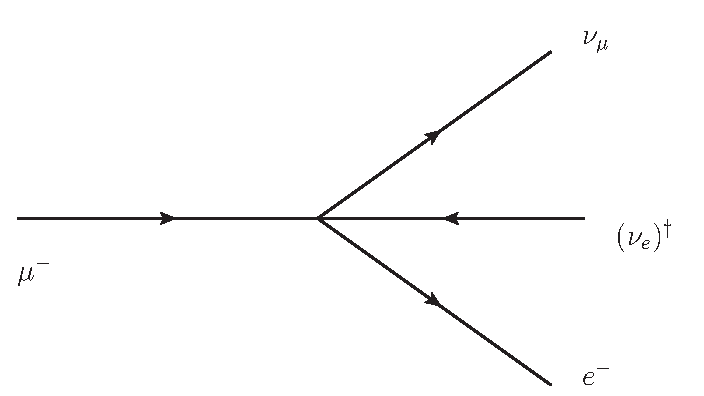
\includegraphics[scale=0.8]{mucontact}  
  \caption{Decaimiento del muón a tres cuerpos}
  \label{fig:mucontact}
\end{figure}

Construyendo la misma interacción a partir del Lagrangiano del ME
\begin{align}
  \mathcal{L}=&\frac{g_2^2}{8}\left[\bar{\nu}_\mu\gamma^\mu(1-\gamma_5)\mu\right] \left[ W_{\mu}^{+}W_\nu^{-} \right]
  \left[\bar{e}\gamma^\nu(1-\gamma_5)\nu_e\right]\,.
\end{align}
Por lo tanto la contracción apropiada de $\left[ W_{\mu}^{+}W_{\nu}^{-} \right]$ debe generar el coeficiente inverso de masa al cuadrado:
\begin{align}
  \left[ W_{\mu}^{+}W_\nu^{-} \right]\to \frac{1}{m_W^2}\,.
\end{align}
Una deducción más rigurosa se realizará en la Sección~\ref{sec:deca-debil-medi}. Por lo tanto
\begin{align}
    \frac{G_F}{\sqrt{2}}=&\frac{g^2}{8m_W^2}\nonumber\\
=& \frac{e^2}{8m_W^2\sin^2\theta_W} \nonumber\\
=& \frac{4\pi e^2}{8(4 \pi) m_W^2\sin^2\theta_W} \nonumber\\
=& \frac{\pi\alpha }{2 m_W^2\sin^2\theta_W} \nonumber\\
m_{W}^2\sin^2\theta_W=&\frac{\sqrt{2}\pi\alpha }{2 G_F} \nonumber\\
m_{W}^2\sin^2\theta_W=&\frac{\pi\alpha }{\sqrt{2} G_F} \,.
\end{align}

Además, de la ec.~\eqref{eq:mwzw}
\begin{align}
  \cos^2\theta_W=&\frac{m_W^2}{m_Z^2} \nonumber\\
  1-\sin^2\theta_W=&\frac{m_W^2}{m_Z^2} \nonumber\\
  \sin^2\theta_W=&1-\frac{m_W^2}{m_Z^2} \,.
\end{align}


De esta forma tenemos las relaciones
\begin{align}
  \sin^2\theta_W=&1-\frac{m_W^2}{m_Z^2}\,,&m_W^2\sin^2\theta_W=\frac{\pi\alpha}{\sqrt{2}G_F}\,,
\end{align}
que permiten determinar que
\begin{align}
  \sin^2\theta_W\approx &0.21\nonumber\\
  m_W\approx &81\,\text{GeV}\,.
\end{align}
El uso de $\alpha(M_Z)\approx1/128$, permite tener en cuenta algunas correcciones cuánticas dando lugar a
\begin{align}
   \sin^2\theta_W\approx &0.23\nonumber\\
  m_W\approx &80\,\text{GeV}
\end{align}
Los valores medidos son $\sin^2\theta_W=0.23149(13)$, $m_W=80.398(25)\,$GeV, y pueden ser reproducidos por el modelo estándar una vez se tienen en cuenta correcciones perturbativas inducidas por partículas virtuales.

El acelerador $e^+e^-$ LEP, que funcionó desde 1998 hasta el 2000~\cite{LEP}, operó a energías suficientes para producir millones de $Z$. Combinado con otros resultados experimentales, se pudo verificar todo el Lagrangiano del Modelo Estándar hasta un nivel del 1 por mil. Con excepción de las interacciones asociadas con el Higgs. 

La universalidad de los decaimientos del $Z$ está soportada por los resultados experimentales siguientes donde sólo se muestran los decaimientos leptónicos del $Z$ diferentes de cero \cite{a} 
\begin{align}
  \label{eq:232qft}
  \Gamma(Z\to e^+e^-)&=83.92(12)\,\text{MeV} &\Gamma(Z\to\mu^+\mu^-)&=83.99(18)\,\text{MeV} 
  &\Gamma(Z\to\tau^+\tau^-)&=84.08(22)\,\text{MeV} \nonumber\\
  \operatorname{Br}(Z\to e^+e^-)&=3.363(4)\%, &\operatorname{Br}(Z\to\mu^+\mu^-)&=3.366(7)\%,  &
  \operatorname{Br}(Z\to\tau^+\tau^-)&=3.370(8)\% 
\end{align}
Mientras que para el $W^\pm$, en \%, \cite{pdg}
\begin{align}
\label{eq:231qft}
  \operatorname{Br}(W^-\to\bar{\nu}_e e^-)&=10.71(16), &
\operatorname{Br}(W^-\to\bar{\nu}_\mu \mu^-)&=10.63(15), &
\operatorname{Br}(W^-\to\bar{\nu}_\tau \tau^-)&=11.38(21)\,. 
\end{align}
La diferencia de $\bar{\nu}_\tau \tau$ respecto a los otros representa un efecto alrededor de $2\sigma$. La universalidad de los acoplamientos leptónicos de $W$ puede comprobarse también indirectamente a través de los decaimientos débiles mediados por corrientes cargadas. Los datos actuales verifican la universalidad de los acoplamientos de corrientes cargadas leptónicas al nivel del 0.2\%~\cite{a}. Sin necesidad de entrar en detalles de los cálculos de las amplitudes de decaimiento, podemos usar el hecho de que ellas son proporcionales a los acoplamientos al cuadrado correspondiente, de modo que  un cociente entre amplitudes de decaimiento es igual, en primera aproximación, a los cocientes de los acoplamientos al cuadrado. Tendremos en cuenta además que el Branching es la amplitud de decaimiento a un canal especifico divido por la suma de las amplitudes de decaimiento a todos los canales posibles.




Para los decaimientos del $Z$ el Modelo Estándar predice, además de la ausencia de eventos del tipo $Z\to e^+\mu^-$, que para un cierto  $l=e,\mu,\tau$, o  $q=d,s,b$
\begin{align}
  \frac{ \operatorname{Br}(Z\to l^+l^-)}{ \operatorname{Br}(Z\to\bar{q}q)}\approx&
\frac{(|v_l|^2+|a_l|^2)}{N_c(|v_q|^2+|a_q|^2)}\nonumber\\
=&\frac{\left[\left(-\frac{1}{2}+2\sin^2\theta_W\right)^2+\frac{1}{4}\right]}{
N_c\left[\left(-\frac{1}{2}+\frac{2}{3}\sin^2\theta_W\right)^2+\frac{1}{4}\right]}\nonumber\\
\approx&\frac{0.776}{N_c}=
\begin{cases}
  0.338& N_c=2\\
  0.225& N_c=3\\
  0.169& N_c=4
\end{cases}
\end{align}
Para ser comparado con el resultado experimental de por ejemplo
\begin{align}
  \frac{ \operatorname{Br}(Z\to e^+e^-)}{ \operatorname{Br}(Z\to\bar{b}b)}=\frac{3.363(4)}{15.12(5)}\approx0.222
\end{align}
que de nuevo da lugar al $N_c=3$, que seguiremos tomando en adelante.

Los Branchings de decaimiento en la ec.~\eqref{eq:231qft} y ec.~\eqref{eq:232qft}  pueden ser calculados sin entrar en detalles del cálculo de las amplitudes. Teniendo en cuenta que el canal $Z\to\bar{t}t$ esta cerrado
\begin{align}
  &\operatorname{Br}(Z\to e^+e^-)=\frac{\Gamma(Z\to e^+e^-)}{\Gamma_{\text{total}}}\nonumber\\
 &\qquad=\frac{(|v_e|^2+|a_e|^2)}{\sum_l[(|v_l|^2+|a_l|^2)+(|v_{\nu_l}|^2+|a_{\nu_l}|^2)]
+N_c[\sum_{i=1}^2(|v_{u_i}|^2+|a_{u_i}|^2)+\sum_{i=1}^3(|v_{d_i}|^2+|a_{d_i}|^2)]}\nonumber\\
 &\qquad=\frac{(|v_e|^2+|a_e|^2)}{3[(|v_e|^2+|a_e|^2)+(|v_{\nu_e}|^2+|a_{\nu_e}|^2)]
+3[2(|v_{u}|^2+|a_{u}|^2)+3(|v_{d}|^2+|a_{d}|^2)]}\nonumber\\
  &\qquad=\frac{(|v_e|^2+|a_e|^2)}{21|a_e|^2+3[|v_e|^2+|v_{\nu_e}|^2]
+3[2|v_{u}|^2+3|v_{d}|^2]}\nonumber\\
 &\qquad=\frac{(-1+4s^2\theta_W)^2+1}{21+3[(-1+4s^2\theta_W)^2+1]
+3[2(1-\frac{8}{3}s^2\theta_W)^2+3(-1+\frac{4}{3}s^2\theta_W)^2]}\nonumber\\
  &\qquad=\frac{2-8s^2\theta_W+16s^4\theta_W}{42-80s^2\theta_W+\frac{320}{3}s^4\theta_W}\nonumber\\
&\qquad\approx3.43\%
\end{align}
Para $W^\pm$ tenemos por ejemplo
\begin{align}
\operatorname{Br}(W^-\to\bar{\nu}_e e^-)=\frac{\Gamma(W^-\to\bar{\nu}_e e^-)}{\Gamma_{\text{total}}}
\end{align}
donde, teniendo en cuenta que los canales a top están cerrados, y usando la condición de unitariedad de la matriz CKM en ec.~\eqref{eq:230qft}, tenemos
\begin{align}
  \Gamma_{\text{total}}=&\sum_l\Gamma(W^-\to\bar{\nu}_l l^-)+N_c\sum_i[\Gamma(W^-\to\bar{u}_1d_i)+\Gamma(W^-\to\bar{u}_2d_i)]\nonumber\\
  =&\Gamma(W^-\to\bar{\nu}_e e^-)\{3+N_c\sum_i[|V_{1i}|^2+|V_{1i}|^2]\} \nonumber\\
  =&\Gamma(W^-\to\bar{\nu}_e e^-)(3+2N_c) \nonumber\\
\end{align}
entonces
\begin{align}
  \operatorname{Br}(W^-\to\bar{\nu}_e e^-)=\frac{1}{3+2N_c}=11.1\%
\end{align}
Una mejor predicción de dichos resultados en el contexto del Modelo Estándar requiere tener en cuenta las correcciones radiativas.


El ME también tiene una predicción concreta para la amplitud del $Z$ a neutrinos, $\Gamma_{\text{inv}}$:
\begin{align}
  \frac{\Gamma_{\text{inv}}}{\Gamma_l}=&\frac{\sum_l\Gamma(Z\to\bar{\nu}_l\nu_l)}{\Gamma(Z\to e^+ e^-)}\nonumber\\
  &=\frac{N_\nu\Gamma(Z\to\bar{\nu}_e\nu_e)}{\Gamma(Z\to e^+ e^-)}\nonumber\\
  &\approx\frac{N_\nu(|v_{\nu_e}|^2+|a_{\nu_e}|^2)}{|v_{e}|^2+|a_{e}|^2}\nonumber\\
  &=\frac{2N_\nu}{(-1+4\sin^2\theta_W)^2+1}\nonumber\\
  &=\frac{N_\nu}{1-4\sin^2\theta_W+8 \sin^4\theta_W}\nonumber\\
  &\approx\begin{cases}
    5.865&N_\nu=3\\
    7.819&N_\nu=4
  \end{cases}\,,
\end{align}
mientras que el valor medido experimentalmente para esta cantidad $5.942(16)$ \cite{a}, es una evidencia muy fuerte de que sólo exiten tres neutrinos livianos. 
\end{frame}

Note que el mismo resultado se puede obtener usuando la notación de dos componentes de \eqref{eq:lsmw}. Con $t_{e_R}=0$, $t_{\nu}=-t_{e_L}=1$, $Q_{\nu}=0$ y $Q_e=-1$ tenemos que
\begin{align}
  \frac{\Gamma_{\text{inv}}}{\Gamma_l}=&\frac{\sum_l\Gamma \left[ Z\to \left( \nu_l \right)^{\dagger}\nu_l \right]}{\Gamma \left[Z\to \left( e_L \right)^{\dagger} e_L  \right]+\Gamma \left[Z\to \left( e_R \right)^{\dagger} e_R  \right]}\nonumber\\
=&\frac{N_{\nu} t_{\nu}^2 }{\left( t_{e_L} - 2 Q_e \sin^2\theta_W \right)^2+ \left( 2 Q_e \sin^2\theta_W \right)^2 } \nonumber\\
=&\frac{N_{\nu} }{\left( -1 + 2 \sin^2\theta_W \right)^2+4 \sin^4\theta_W } \nonumber\\
=&\frac{N_{\nu} }{1 - 4 \sin^2\theta_W +4 \sin^4\theta_W +4 \sin^4\theta_W } \nonumber\\
=&\frac{N_{\nu} }{1 - 4 \sin^2\theta_W +8 \sin^4\theta_W } \,.
\end{align}

\subsection{Decaimientos débiles mediados por corrientes cargadas}
\label{sec:deca-debil-medi}
\begin{frame}[fragile,allowframebreaks]
De la corrientes cargadas para leptones tenemos
\begin{align}
  \mathcal{L}_{cc}\supset&\frac{g_2}{2\sqrt{2}}\left[\sum_l\bar{\nu_l}\gamma^\mu(1-\gamma_5)l W_\mu^++\bar{l}\gamma^\mu(1-\gamma_5)\nu_l W_\mu^-\right]
\end{align}
Esto da lugar a los posibles diagramas para decaimientos de leptones a bosones virtuales, y bosones a leptontes mostrados en la figura~\ref{fig:leptoncc}. Las flechas representan el flujo de número leptónico. La flecha de tiempo es de izquierda a derecha. Al lado izquierdo del vértice entran partículas y salen antipartículas. Mientras que al lado derecho entran antip artículas y salen partículas
\begin{figure}
  \centering
  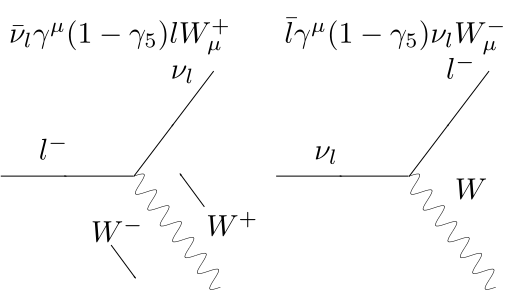
\includegraphics[scale=0.5]{leptoncc}
\qquad  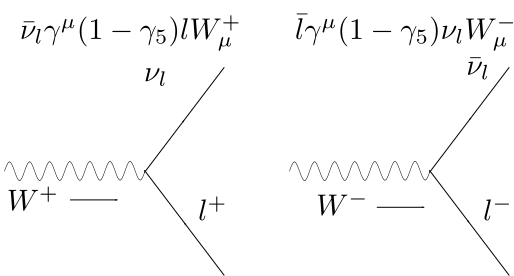
\includegraphics[scale=0.5]{wdecay}

  \caption{Diagramas de Feynman para las corrientes cargadas}
  \label{fig:leptoncc}
\end{figure}
Del primer y cuarto diagrama obtenemos el diagrama de Feynman para el decaimiento $\mu^-\to \nu_\mu e^-\bar{\nu}_e$, mostrado en la figura~\ref{fig:muondecay}
\begin{figure}
  \centering
  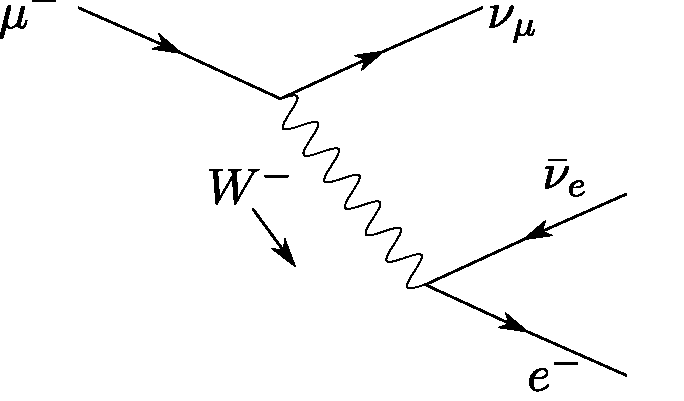
\includegraphics[scale=0.5]{muon_decay}
  \caption{diagrama de Feynman para el decaimiento $\mu^-\to \nu_\mu e^-\bar{\nu}_e$}
  \label{fig:muondecay}
\end{figure}
El propagador para el bosón $W$ de momentum $q$ resulta ser
\begin{align}
  \widetilde{D}_{\mu\nu}=\frac{1}{q^2-m_W^2}\left(g_{\mu\nu}-\frac{q_\mu q_\nu}{m_W^2}\right)\,.
\end{align}
Para los propósitos actuales la obtención de este resultado no es necesaria, el punto importante es que cuando los momentum de las partículas iniciales y finales son mucho más pequeñas que $m_W$, esto se reduce a
\begin{align}
  \widetilde{D}_{\mu\nu}=-\frac{g_{\mu\nu}}{m_W^2}\,.
\end{align}
Este resultado se entiende fácilmente cuando se compara con el propagador de una partículas escalar masiva $1/(q^2-M^2)\to-1/M^2$. Las componentes espaciales de $W_\mu$ con $\mu=1,2,3$, a bajas energías tienen el mismo propagador que el de una partícula escalar, mientras $W_0$, tiene el signo opuesto.

El Lagrangiano efectivo para el decaimiento del muón, $\mu^-\to \nu_\mu e^- \bar{\nu}_e$ es entonces
\begin{align}
  \mathcal{L}=&\frac{g_2^2}{8}\left[\bar{\nu}_\mu\gamma^\mu(1-\gamma_5)\mu\right]\frac{g_{\mu\nu}}{m_W^2}
  \left[\bar{e}\gamma^\nu(1-\gamma_5)\nu_e\right]\nonumber\\
=&\frac{g_2^2}{8m_W^2}\left[\bar{\nu}_\mu\gamma^\mu(1-\gamma_5)\mu\right]
  \left[\bar{e}\gamma^\nu(1-\gamma_5)\nu_e\right]\nonumber\\
  =&\frac{G_F}{\sqrt{2}}\left[\bar{\nu}_\mu\gamma^\mu(1-\gamma_5)\mu\right]\left[\bar{e}\gamma_\mu(1-\gamma_5)\nu_e\right]\,,
\end{align}
donde
\begin{align}
  \frac{G_F}{\sqrt{2}}=&\frac{g_2^2}{8m_W^2}\nonumber\\
  =&\frac{g_2^24}{8g^2v^2}\nonumber\\
  =&\frac{1}{2v^2}\,,
\end{align}
y
\begin{align}
  v=\left(\sqrt{2}\,G_F\right)^{-1/2}=&246.2\ \text{GeV}\nonumber\\
 \approx&2.9\times 10^{15}\ \text{K} \nonumber\\
 \approx&4.9\times 10^{-14}\ \text{m} \nonumber\\
 \approx&1.6\times 10^{-22}\ \text{s} \,.
\end{align}


De otro lado, para el  decaimiento $\beta$, $n\to p e^- \bar{\nu}_e$, de acuerdo a la figura~\ref{fig:neutrondecay}, tenemos

\begin{align}
    \mathcal{L}=\frac{G_\beta}{\sqrt{2}}\left[\bar{p}\gamma^\mu(1-1.26\gamma_5)n\right]\left[\bar{e}\gamma_\mu(1-\gamma_5)\nu_e\right]\,.
\end{align}
\begin{figure}
  \centering
  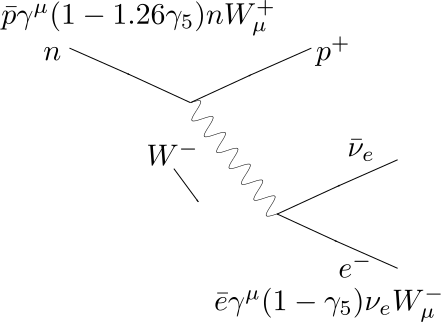
\includegraphics[scale=0.5]{neutrondecay}
  \caption{Decaimiento del neutrón.}
  \label{fig:neutrondecay}
\end{figure}
con $G_F$ dado en la ec.~\eqref{eq:233qft} y $G_\beta=1.10\times 10^{-5}\,\text{GeV}^2$. La corriente hadrónica tiene la forma V--1.26A. El factor 1.26  puede entenderse como debido a las correcciones a nivel hadrónico de una corriente que es de la forma V--A a nivel del quarks, como en la ec.~\eqref{eq:234qft}. A nivel de quarks el decaimiento del neutrón ($udd$) al protón ($uud$) corresponde al decaimiento de uno de los quarks down del neutrón $d\to u e^- \bar{\nu}_e$
\begin{align}
    \mathcal{L}=\frac{G_F}{\sqrt{2}}V_{11}\left[\bar{u}\gamma^\mu(1-\gamma_5)d\right]\left[\bar{e}\gamma_\mu(1-\gamma_5)\nu_e\right]\,.
\end{align}
De modo que $G_\beta=G_F V_{11}=G_F\cos\theta_C$, donde $\theta_C$ es el ángulo de Cabbibo. Una vez se tienen en cuenta correcciones electrodébiles se obtiene el valor $|V_{11}|=0.97418(27)$\cite{PDG}. Las magnitudes de los elementos de la matriz CKM son\cite{PDG}
\begin{align}
  V\approx\begin{pmatrix}
    0.97419&0.2257&0.0359\\
    0.2256&0.97334&0.0415\\
    0.00874&0.0407&0.999133
  \end{pmatrix}\sim \mathbf{1}
\end{align}
\end{frame}

Para cerrar esta notas, transcribo a continuación el último párrafo de la conferencia de Steven Weinberg en 1979 con motivo de la entrega del premio nobel del física por el desarrollo del modelo estándar de las interacciones fundamentales:

\begin{quote}
[...]  And
nothing makes me more optimistic than the discovery of broken symmetries.
In the seventh book of the Republic, Plato describes prisoners who are
chained in a cave and can see only shadows that things outside cast on the
cave wall. When released from the cave at first their eyes hurt, and for a
while they think that the shadows they saw in the cave are more real than
the objects they now see. But eventually their vision clears, and they can
understand how beautiful the real world is. We are in such a cave, imprisoned
by the limitations on the sorts of experiments we can do. In particular,
we can study matter only at relatively low temperatures, where symmetries
are likely to be spontaneously broken, so that nature does not appear
very simple or unified. We have not been able to get out of this cave, but by
looking long and hard at the shadows on the cave wall, we can at least make
out the shapes of symmetries, which though broken, are exact principles
governing all phenomena, expressions of the beauty of the world outside.
\end{quote}
S. Weinberg, Nobel lecture, 1979

\section{Resumen}
A modo de resumén, usaremos a continuación la siguiente secuencia de la historieta de \url{http://www.phdcomics.com} re-explicando el bosón de Higgs:
\newpage

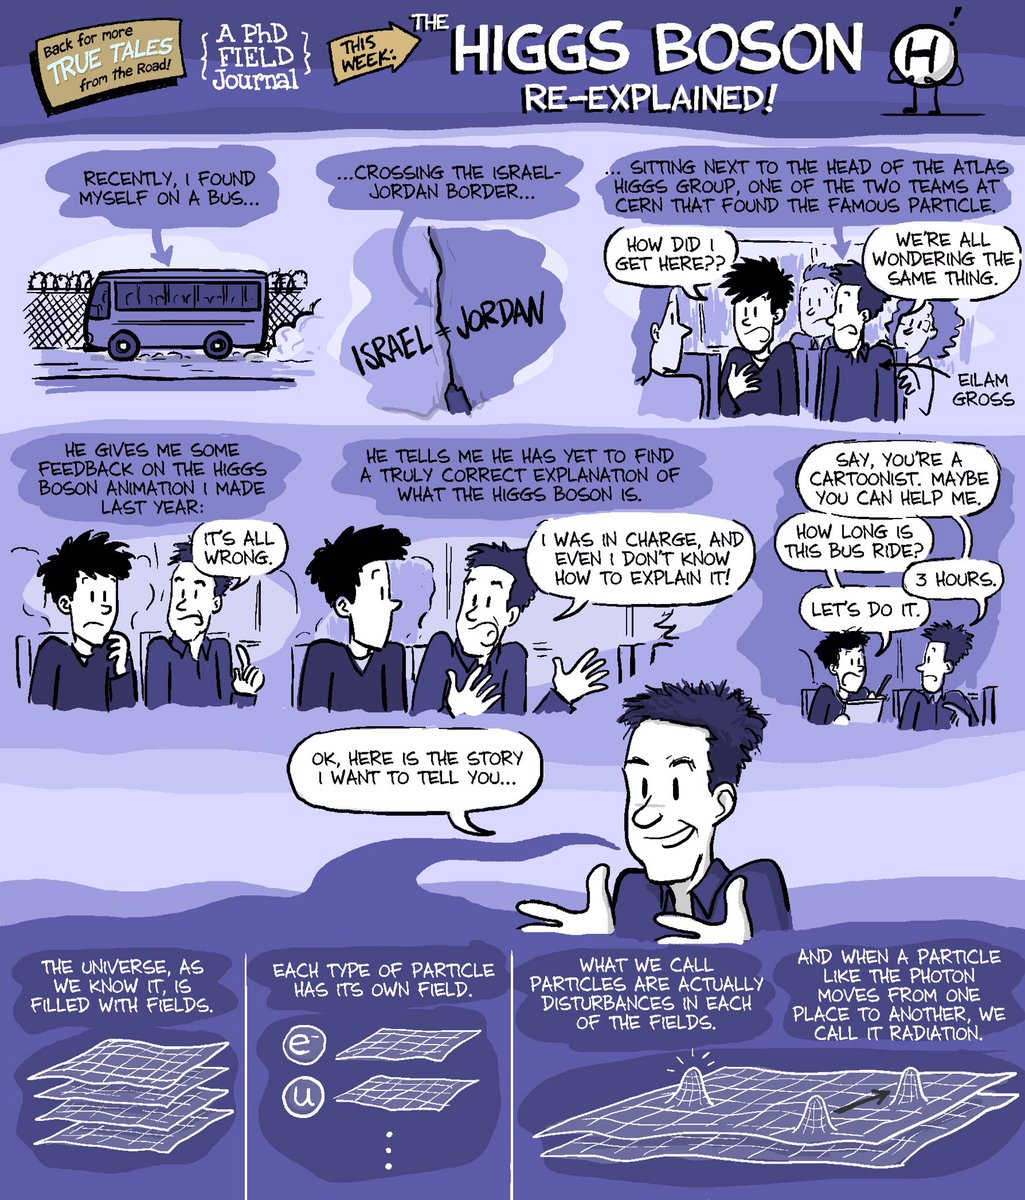
\includegraphics[scale=0.51]{Higgs1}

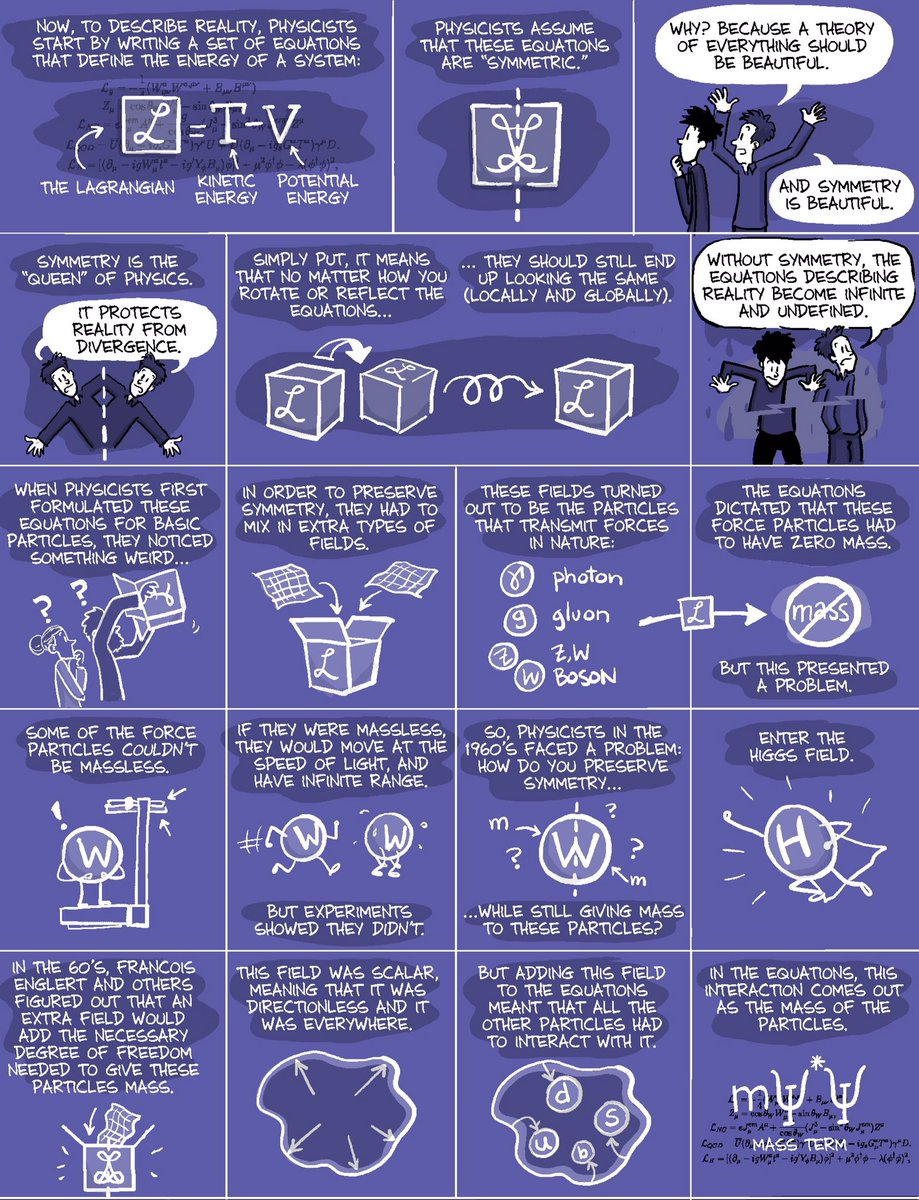
\includegraphics[scale=0.56]{Higgs2}

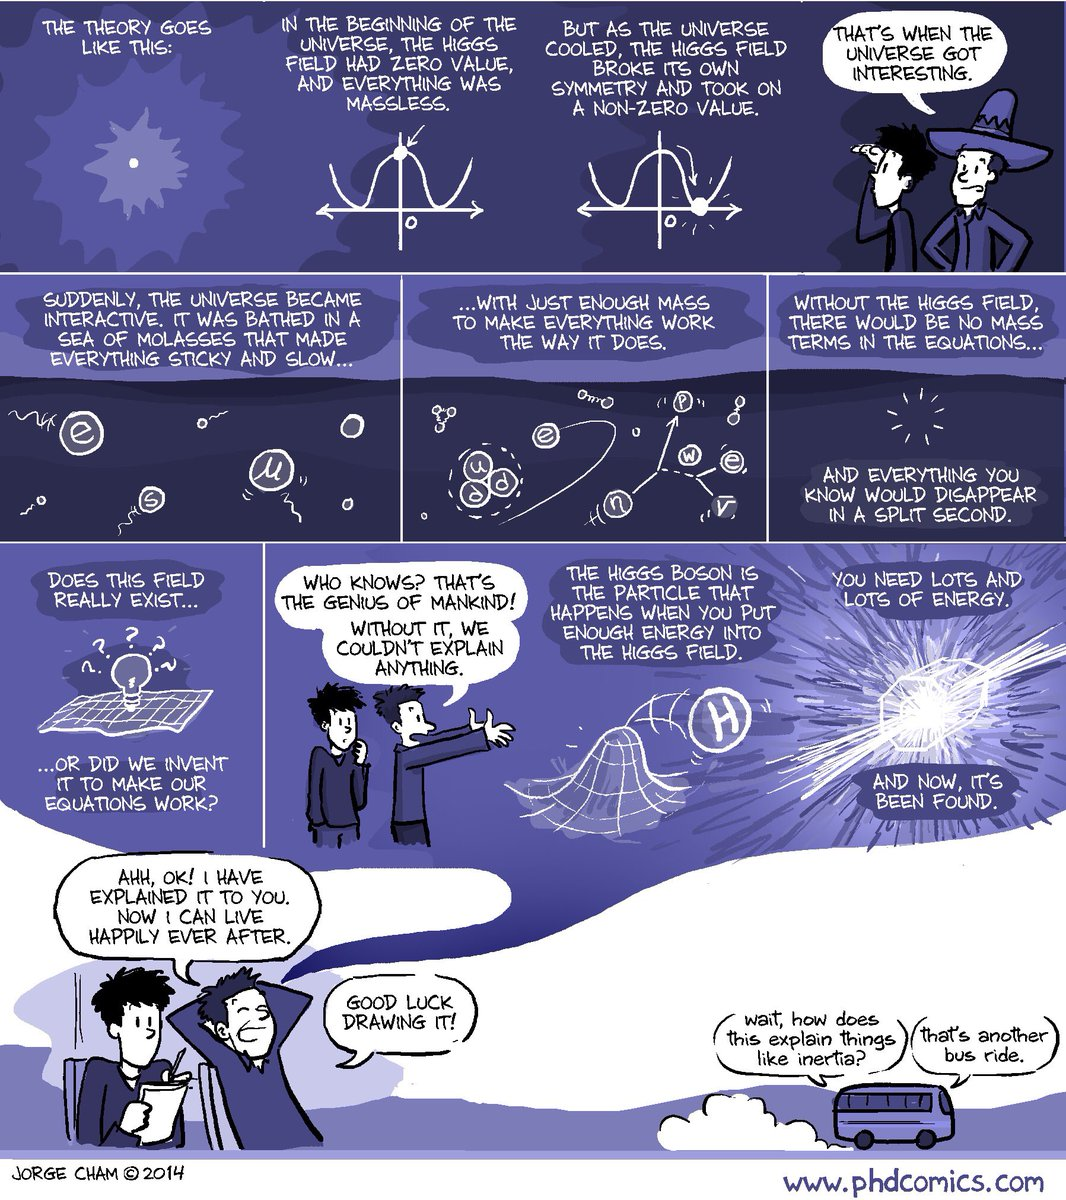
\includegraphics[scale=0.49]{Higgs3}

\newpage


\section{Lecturas recomendadas}
Libros:
\begin{itemize}
\item \cite{kane,cottingham,Pich:2005mk}
\end{itemize}

Artículos originales

\begin{itemize}
\item Teorías no abelianas \cite{Yang:1954ek}
\item Mecanismo de Higgs \cite{Higgs:1964pj}
\item Teoría electrodébil \cite{Weinberg:1967tq}
\end{itemize}

Artículo de divulgación
\begin{itemize}
\item The deconstructed Standard Model equation, Rashmi Shivni \url{https://www.symmetrymagazine.org/article/the-deconstructed-standard-model-equation}
\end{itemize}

Videos:
\begin{itemize}
\item Strange Stars Explained: \url{https://www.youtube.com/watch?v=p_8yK2kmxoo}
\end{itemize}

% \left(\right)
%
%%% Local Variables: 
%%% mode: latex
%%% TeX-master: "fullnotes"
%%% ispell-local-dictionary: "castellano8"
%%% End:
}

\end{document}

%TEMPLATES:

\chapter{Hola}
\section{Introduction}
This is the introduction text. This text is not shown in the
presentation, but will be part of the article.
\begin{frame}
Hola mundo
\end{frame}
This text is once more not shown in the presentation.
\section{Main Part}
While this text is not shown in the presentation, the section command
also applies to the presentation.
We can add a subsection that is only part of the article like this:
\subsection<article>{Article-Only Section}
With some more text.
\begin{frame}
This text is part both of the article and of the presentation.
\begin{itemize}
\item This stuff is also shown in both version.
\item This too.
\only<article>{\item This particular item is only part
of the article version.}
\item<presentation:only@0> This text is also only part of the article.
\end{itemize}

\end{frame}

Templates:
%%%tablas de colores
\mode<presentation>{\rowcolors{1}{RoyalBlue!20}{}}

\begin{frame}[fragile,allowframebreaks]
\end{frame}

%numbers in beamer
\begin{lstlisting}[numbers=left,xleftmargin=1cm,numberstyle=\tiny,escapeinside={(*}{*)}]
\end{lstlisting}


\begin{pyprogram}
\lstset{numbers=left}
\begin{lstlisting}[label=XXX,caption=XXX]
\end{lstlisting}
\end{pyprogram}

\begin{pyprogram}
\mode<presentation>{\lstset{basicstyle=\tiny\ttfamily}}
\filetitle{cinematica.py}
\lstinputlisting{python/programas/cinematica/cinematica.py}
\end{pyprogram}



\begin{ipython}
\begin{lstlisting}[title=]
In [1]:
\end{lstlisting}
\end{ipython}

\begin{terminal}
\begin{lstlisting}[title=1]

\end{lstlisting}
\end{terminal}

\begin{columns}
  \begin{column}{0.5\textwidth}
    
  \end{column}
  \begin{column}{0.5\textwidth}
    
  \end{column}
\end{columns}


%%% Local Variables: 
%%% mode: latex
%%% TeX-master: "beyond.beamer.tex"
%%% End: